\documentclass[twoside]{book}

% Packages required by doxygen
\usepackage{fixltx2e}
\usepackage{calc}
\usepackage{doxygen}
\usepackage[export]{adjustbox} % also loads graphicx
\usepackage{graphicx}
\usepackage[utf8]{inputenc}
\usepackage{makeidx}
\usepackage{multicol}
\usepackage{multirow}
\PassOptionsToPackage{warn}{textcomp}
\usepackage{textcomp}
\usepackage[nointegrals]{wasysym}
\usepackage[table]{xcolor}

% Font selection
\usepackage[T1]{fontenc}
\usepackage[scaled=.90]{helvet}
\usepackage{courier}
\usepackage{amssymb}
\usepackage{sectsty}
\renewcommand{\familydefault}{\sfdefault}
\allsectionsfont{%
  \fontseries{bc}\selectfont%
  \color{darkgray}%
}
\renewcommand{\DoxyLabelFont}{%
  \fontseries{bc}\selectfont%
  \color{darkgray}%
}
\newcommand{\+}{\discretionary{\mbox{\scriptsize$\hookleftarrow$}}{}{}}

% Page & text layout
\usepackage{geometry}
\geometry{%
  a4paper,%
  top=2.5cm,%
  bottom=2.5cm,%
  left=2.5cm,%
  right=2.5cm%
}
\tolerance=750
\hfuzz=15pt
\hbadness=750
\setlength{\emergencystretch}{15pt}
\setlength{\parindent}{0cm}
\setlength{\parskip}{3ex plus 2ex minus 2ex}
\makeatletter
\renewcommand{\paragraph}{%
  \@startsection{paragraph}{4}{0ex}{-1.0ex}{1.0ex}{%
    \normalfont\normalsize\bfseries\SS@parafont%
  }%
}
\renewcommand{\subparagraph}{%
  \@startsection{subparagraph}{5}{0ex}{-1.0ex}{1.0ex}{%
    \normalfont\normalsize\bfseries\SS@subparafont%
  }%
}
\makeatother

% Headers & footers
\usepackage{fancyhdr}
\pagestyle{fancyplain}
\fancyhead[LE]{\fancyplain{}{\bfseries\thepage}}
\fancyhead[CE]{\fancyplain{}{}}
\fancyhead[RE]{\fancyplain{}{\bfseries\leftmark}}
\fancyhead[LO]{\fancyplain{}{\bfseries\rightmark}}
\fancyhead[CO]{\fancyplain{}{}}
\fancyhead[RO]{\fancyplain{}{\bfseries\thepage}}
\fancyfoot[LE]{\fancyplain{}{}}
\fancyfoot[CE]{\fancyplain{}{}}
\fancyfoot[RE]{\fancyplain{}{\bfseries\scriptsize 構築\+: Doxygen }}
\fancyfoot[LO]{\fancyplain{}{\bfseries\scriptsize 構築\+: Doxygen }}
\fancyfoot[CO]{\fancyplain{}{}}
\fancyfoot[RO]{\fancyplain{}{}}
\renewcommand{\footrulewidth}{0.4pt}
\renewcommand{\chaptermark}[1]{%
  \markboth{#1}{}%
}
\renewcommand{\sectionmark}[1]{%
  \markright{\thesection\ #1}%
}

% Indices & bibliography
\usepackage{natbib}
\usepackage[titles]{tocloft}
\setcounter{tocdepth}{3}
\setcounter{secnumdepth}{5}
\makeindex

% Hyperlinks (required, but should be loaded last)
\usepackage{ifpdf}
\ifpdf
  \usepackage[pdftex,pagebackref=true]{hyperref}
\else
  \usepackage[ps2pdf,pagebackref=true]{hyperref}
\fi
\hypersetup{%
  colorlinks=true,%
  linkcolor=blue,%
  citecolor=blue,%
  unicode%
}

% Custom commands
\newcommand{\clearemptydoublepage}{%
  \newpage{\pagestyle{empty}\cleardoublepage}%
}

\usepackage{caption}
\captionsetup{labelsep=space,justification=centering,font={bf},singlelinecheck=off,skip=4pt,position=top}

%===== C O N T E N T S =====

\begin{document}

% Titlepage & ToC
\hypersetup{pageanchor=false,
             bookmarksnumbered=true,
             pdfencoding=unicode
            }
\pagenumbering{alph}
\begin{titlepage}
\vspace*{7cm}
\begin{center}%
{\Large R\+C\+R\+S-\/\+A\+DF }\\
\vspace*{1cm}
{\large 構築\+: Doxygen 1.8.12}\\
\end{center}
\end{titlepage}
\clearemptydoublepage
\pagenumbering{roman}
\tableofcontents
\clearemptydoublepage
\pagenumbering{arabic}
\hypersetup{pageanchor=true}

%--- Begin generated contents ---
\chapter{非推奨一覧}
\label{deprecated}
\hypertarget{deprecated}{}

\begin{DoxyRefList}
\item[\label{deprecated__deprecated000001}%
\hypertarget{deprecated__deprecated000001}{}%
クラス \hyperlink{classadf_1_1agent_1_1communication_1_1standard_1_1bundle_1_1topdown_1_1CommandAmbulance}{adf.agent.communication.standard.bundle.topdown.Command\+Ambulance} ]change class name \hyperlink{classadf_1_1agent_1_1communication_1_1standard_1_1bundle_1_1centralized_1_1CommandAmbulance}{adf.\+agent.\+communication.\+standard.\+bundle.\+centralized.\+Command\+Ambulance}  
\item[\label{deprecated__deprecated000002}%
\hypertarget{deprecated__deprecated000002}{}%
クラス \hyperlink{classadf_1_1agent_1_1communication_1_1standard_1_1bundle_1_1topdown_1_1CommandFire}{adf.agent.communication.standard.bundle.topdown.Command\+Fire} ]change class name \hyperlink{classadf_1_1agent_1_1communication_1_1standard_1_1bundle_1_1centralized_1_1CommandFire}{adf.\+agent.\+communication.\+standard.\+bundle.\+centralized.\+Command\+Fire}  
\item[\label{deprecated__deprecated000003}%
\hypertarget{deprecated__deprecated000003}{}%
クラス \hyperlink{classadf_1_1agent_1_1communication_1_1standard_1_1bundle_1_1topdown_1_1CommandPolice}{adf.agent.communication.standard.bundle.topdown.Command\+Police} ]change class name \hyperlink{classadf_1_1agent_1_1communication_1_1standard_1_1bundle_1_1centralized_1_1CommandPolice}{adf.\+agent.\+communication.\+standard.\+bundle.\+centralized.\+Command\+Police}  
\item[\label{deprecated__deprecated000004}%
\hypertarget{deprecated__deprecated000004}{}%
クラス \hyperlink{classadf_1_1agent_1_1communication_1_1standard_1_1bundle_1_1topdown_1_1CommandScout}{adf.agent.communication.standard.bundle.topdown.Command\+Scout} ]change class name \hyperlink{classadf_1_1agent_1_1communication_1_1standard_1_1bundle_1_1centralized_1_1CommandScout}{adf.\+agent.\+communication.\+standard.\+bundle.\+centralized.\+Command\+Scout}  
\item[\label{deprecated__deprecated000005}%
\hypertarget{deprecated__deprecated000005}{}%
クラス \hyperlink{classadf_1_1agent_1_1communication_1_1standard_1_1bundle_1_1topdown_1_1MessageReport}{adf.agent.communication.standard.bundle.topdown.Message\+Report} ]change class name \hyperlink{classadf_1_1agent_1_1communication_1_1standard_1_1bundle_1_1centralized_1_1MessageReport}{adf.\+agent.\+communication.\+standard.\+bundle.\+centralized.\+Message\+Report}  
\item[\label{deprecated__deprecated000006}%
\hypertarget{deprecated__deprecated000006}{}%
メンバ \hyperlink{classadf_1_1component_1_1AbstractLoader_a2044c317869b16349d4fdbf7d5d50dcd}{adf.component.Abstract\+Loader.get\+Control\+Ambulance} ()]change method name \hyperlink{}{get\+Tactics\+Ambulance\+Center()}  
\item[\label{deprecated__deprecated000007}%
\hypertarget{deprecated__deprecated000007}{}%
メンバ \hyperlink{classadf_1_1component_1_1AbstractLoader_a66e4649d775d291dda3e5b977596bccf}{adf.component.Abstract\+Loader.get\+Control\+Fire} ()]change method name \hyperlink{}{get\+Tactics\+Fire\+Center()}  
\item[\label{deprecated__deprecated000008}%
\hypertarget{deprecated__deprecated000008}{}%
メンバ \hyperlink{classadf_1_1component_1_1AbstractLoader_a2917adfedf677a3af006521e64996a42}{adf.component.Abstract\+Loader.get\+Control\+Police} ()]change method name \hyperlink{}{get\+Tactics\+Police\+Center()}  
\item[\label{deprecated__deprecated000009}%
\hypertarget{deprecated__deprecated000009}{}%
クラス \hyperlink{classadf_1_1component_1_1control_1_1Control}{adf.component.control.Control} ]change class name \hyperlink{}{Tactics\+Center}  
\item[\label{deprecated__deprecated000010}%
\hypertarget{deprecated__deprecated000010}{}%
クラス \hyperlink{classadf_1_1component_1_1control_1_1ControlAmbulance}{adf.component.control.Control\+Ambulance} ]change class name \hyperlink{}{Tactics\+Ambulance\+Center}  
\item[\label{deprecated__deprecated000011}%
\hypertarget{deprecated__deprecated000011}{}%
クラス \hyperlink{classadf_1_1component_1_1control_1_1ControlFire}{adf.component.control.Control\+Fire} ]change class name \hyperlink{}{Tactics\+Fire\+Center}  
\item[\label{deprecated__deprecated000012}%
\hypertarget{deprecated__deprecated000012}{}%
クラス \hyperlink{classadf_1_1component_1_1control_1_1ControlPolice}{adf.component.control.Control\+Police} ]change class name \hyperlink{}{Tactics\+Police\+Center}  
\item[\label{deprecated__deprecated000013}%
\hypertarget{deprecated__deprecated000013}{}%
クラス \hyperlink{classadf_1_1component_1_1module_1_1complex_1_1BuildingSelector}{adf.component.module.complex.Building\+Selector} ]change class name \hyperlink{classadf_1_1component_1_1module_1_1complex_1_1BuildingDetector}{Building\+Detector}  
\item[\label{deprecated__deprecated000014}%
\hypertarget{deprecated__deprecated000014}{}%
クラス \hyperlink{classadf_1_1component_1_1module_1_1complex_1_1HumanSelector}{adf.component.module.complex.Human\+Selector} ]change class name \hyperlink{classadf_1_1component_1_1module_1_1complex_1_1HumanDetector}{Human\+Detector}  
\item[\label{deprecated__deprecated000015}%
\hypertarget{deprecated__deprecated000015}{}%
クラス \hyperlink{classadf_1_1component_1_1module_1_1complex_1_1RoadSelector}{adf.component.module.complex.Road\+Selector} ]change class name \hyperlink{classadf_1_1component_1_1module_1_1complex_1_1RoadDetector}{Road\+Detector}  
\item[\label{deprecated__deprecated000016}%
\hypertarget{deprecated__deprecated000016}{}%
クラス \hyperlink{classadf_1_1component_1_1module_1_1complex_1_1TargetSelector}{adf.component.module.complex.Target\+Selector$<$ E extends Standard\+Entity $>$} ]change class name \hyperlink{classadf_1_1component_1_1module_1_1complex_1_1TargetDetector}{Target\+Detector} 
\end{DoxyRefList}
\chapter{階層索引}
\section{Class Hierarchy}
This inheritance list is sorted roughly, but not completely, alphabetically\+:\begin{DoxyCompactList}
\item \contentsline{section}{adf.\+component.\+Abstract\+Loader}{\pageref{classadf_1_1component_1_1AbstractLoader}}{}
\item \contentsline{section}{adf.\+component.\+module.\+Abstract\+Module}{\pageref{classadf_1_1component_1_1module_1_1AbstractModule}}{}
\begin{DoxyCompactList}
\item \contentsline{section}{adf.\+component.\+module.\+algorithm.\+Clustering}{\pageref{classadf_1_1component_1_1module_1_1algorithm_1_1Clustering}}{}
\begin{DoxyCompactList}
\item \contentsline{section}{adf.\+component.\+module.\+algorithm.\+Dynamic\+Clustering}{\pageref{classadf_1_1component_1_1module_1_1algorithm_1_1DynamicClustering}}{}
\item \contentsline{section}{adf.\+component.\+module.\+algorithm.\+Static\+Clustering}{\pageref{classadf_1_1component_1_1module_1_1algorithm_1_1StaticClustering}}{}
\end{DoxyCompactList}
\item \contentsline{section}{adf.\+component.\+module.\+algorithm.\+Path\+Planning}{\pageref{classadf_1_1component_1_1module_1_1algorithm_1_1PathPlanning}}{}
\item \contentsline{section}{adf.\+component.\+module.\+complex.\+center.\+Target\+Allocation}{\pageref{classadf_1_1component_1_1module_1_1complex_1_1center_1_1TargetAllocation}}{}
\begin{DoxyCompactList}
\item \contentsline{section}{adf.\+component.\+module.\+complex.\+center.\+Ambulance\+Target\+Allocation}{\pageref{classadf_1_1component_1_1module_1_1complex_1_1center_1_1AmbulanceTargetAllocation}}{}
\item \contentsline{section}{adf.\+component.\+module.\+complex.\+center.\+Fire\+Target\+Allocation}{\pageref{classadf_1_1component_1_1module_1_1complex_1_1center_1_1FireTargetAllocation}}{}
\item \contentsline{section}{adf.\+component.\+module.\+complex.\+center.\+Police\+Target\+Allocation}{\pageref{classadf_1_1component_1_1module_1_1complex_1_1center_1_1PoliceTargetAllocation}}{}
\end{DoxyCompactList}
\item \contentsline{section}{adf.\+component.\+module.\+complex.\+Target\+Detector$<$ E extends Standard\+Entity $>$}{\pageref{classadf_1_1component_1_1module_1_1complex_1_1TargetDetector}}{}
\end{DoxyCompactList}
\item \contentsline{section}{adf.\+agent.\+action.\+Action}{\pageref{classadf_1_1agent_1_1action_1_1Action}}{}
\begin{DoxyCompactList}
\item \contentsline{section}{adf.\+agent.\+action.\+ambulance.\+Action\+Load}{\pageref{classadf_1_1agent_1_1action_1_1ambulance_1_1ActionLoad}}{}
\item \contentsline{section}{adf.\+agent.\+action.\+ambulance.\+Action\+Rescue}{\pageref{classadf_1_1agent_1_1action_1_1ambulance_1_1ActionRescue}}{}
\item \contentsline{section}{adf.\+agent.\+action.\+ambulance.\+Action\+Unload}{\pageref{classadf_1_1agent_1_1action_1_1ambulance_1_1ActionUnload}}{}
\item \contentsline{section}{adf.\+agent.\+action.\+common.\+Action\+Move}{\pageref{classadf_1_1agent_1_1action_1_1common_1_1ActionMove}}{}
\item \contentsline{section}{adf.\+agent.\+action.\+common.\+Action\+Rest}{\pageref{classadf_1_1agent_1_1action_1_1common_1_1ActionRest}}{}
\item \contentsline{section}{adf.\+agent.\+action.\+fire.\+Action\+Extinguish}{\pageref{classadf_1_1agent_1_1action_1_1fire_1_1ActionExtinguish}}{}
\item \contentsline{section}{adf.\+agent.\+action.\+fire.\+Action\+Refill}{\pageref{classadf_1_1agent_1_1action_1_1fire_1_1ActionRefill}}{}
\item \contentsline{section}{adf.\+agent.\+action.\+police.\+Action\+Clear}{\pageref{classadf_1_1agent_1_1action_1_1police_1_1ActionClear}}{}
\end{DoxyCompactList}
\item \contentsline{section}{adf.\+agent.\+Agent$<$ E $>$}{\pageref{classadf_1_1agent_1_1Agent}}{}
\item \contentsline{section}{adf.\+agent.\+info.\+Agent\+Info}{\pageref{classadf_1_1agent_1_1info_1_1AgentInfo}}{}
\item \contentsline{section}{adf.\+launcher.\+Agent\+Launcher}{\pageref{classadf_1_1launcher_1_1AgentLauncher}}{}
\item \contentsline{section}{adf.\+component.\+communication.\+util.\+Bit\+Stream\+Reader}{\pageref{classadf_1_1component_1_1communication_1_1util_1_1BitStreamReader}}{}
\item \contentsline{section}{adf.\+component.\+command.\+Command\+Generator}{\pageref{classadf_1_1component_1_1command_1_1CommandGenerator}}{}
\item \contentsline{section}{adf.\+component.\+communication.\+Communication\+Message}{\pageref{classadf_1_1component_1_1communication_1_1CommunicationMessage}}{}
\begin{DoxyCompactList}
\item \contentsline{section}{adf.\+agent.\+communication.\+standard.\+bundle.\+Standard\+Message}{\pageref{classadf_1_1agent_1_1communication_1_1standard_1_1bundle_1_1StandardMessage}}{}
\begin{DoxyCompactList}
\item \contentsline{section}{adf.\+agent.\+communication.\+standard.\+bundle.\+centralized.\+Command\+Ambulance}{\pageref{classadf_1_1agent_1_1communication_1_1standard_1_1bundle_1_1centralized_1_1CommandAmbulance}}{}
\begin{DoxyCompactList}
\item \contentsline{section}{adf.\+agent.\+communication.\+standard.\+bundle.\+topdown.\+Command\+Ambulance}{\pageref{classadf_1_1agent_1_1communication_1_1standard_1_1bundle_1_1topdown_1_1CommandAmbulance}}{}
\end{DoxyCompactList}
\item \contentsline{section}{adf.\+agent.\+communication.\+standard.\+bundle.\+centralized.\+Command\+Fire}{\pageref{classadf_1_1agent_1_1communication_1_1standard_1_1bundle_1_1centralized_1_1CommandFire}}{}
\begin{DoxyCompactList}
\item \contentsline{section}{adf.\+agent.\+communication.\+standard.\+bundle.\+topdown.\+Command\+Fire}{\pageref{classadf_1_1agent_1_1communication_1_1standard_1_1bundle_1_1topdown_1_1CommandFire}}{}
\end{DoxyCompactList}
\item \contentsline{section}{adf.\+agent.\+communication.\+standard.\+bundle.\+centralized.\+Command\+Police}{\pageref{classadf_1_1agent_1_1communication_1_1standard_1_1bundle_1_1centralized_1_1CommandPolice}}{}
\begin{DoxyCompactList}
\item \contentsline{section}{adf.\+agent.\+communication.\+standard.\+bundle.\+topdown.\+Command\+Police}{\pageref{classadf_1_1agent_1_1communication_1_1standard_1_1bundle_1_1topdown_1_1CommandPolice}}{}
\end{DoxyCompactList}
\item \contentsline{section}{adf.\+agent.\+communication.\+standard.\+bundle.\+centralized.\+Command\+Scout}{\pageref{classadf_1_1agent_1_1communication_1_1standard_1_1bundle_1_1centralized_1_1CommandScout}}{}
\begin{DoxyCompactList}
\item \contentsline{section}{adf.\+agent.\+communication.\+standard.\+bundle.\+topdown.\+Command\+Scout}{\pageref{classadf_1_1agent_1_1communication_1_1standard_1_1bundle_1_1topdown_1_1CommandScout}}{}
\end{DoxyCompactList}
\item \contentsline{section}{adf.\+agent.\+communication.\+standard.\+bundle.\+centralized.\+Message\+Report}{\pageref{classadf_1_1agent_1_1communication_1_1standard_1_1bundle_1_1centralized_1_1MessageReport}}{}
\begin{DoxyCompactList}
\item \contentsline{section}{adf.\+agent.\+communication.\+standard.\+bundle.\+topdown.\+Message\+Report}{\pageref{classadf_1_1agent_1_1communication_1_1standard_1_1bundle_1_1topdown_1_1MessageReport}}{}
\end{DoxyCompactList}
\item \contentsline{section}{adf.\+agent.\+communication.\+standard.\+bundle.\+information.\+Message\+Ambulance\+Team}{\pageref{classadf_1_1agent_1_1communication_1_1standard_1_1bundle_1_1information_1_1MessageAmbulanceTeam}}{}
\item \contentsline{section}{adf.\+agent.\+communication.\+standard.\+bundle.\+information.\+Message\+Building}{\pageref{classadf_1_1agent_1_1communication_1_1standard_1_1bundle_1_1information_1_1MessageBuilding}}{}
\item \contentsline{section}{adf.\+agent.\+communication.\+standard.\+bundle.\+information.\+Message\+Civilian}{\pageref{classadf_1_1agent_1_1communication_1_1standard_1_1bundle_1_1information_1_1MessageCivilian}}{}
\item \contentsline{section}{adf.\+agent.\+communication.\+standard.\+bundle.\+information.\+Message\+Fire\+Brigade}{\pageref{classadf_1_1agent_1_1communication_1_1standard_1_1bundle_1_1information_1_1MessageFireBrigade}}{}
\item \contentsline{section}{adf.\+agent.\+communication.\+standard.\+bundle.\+information.\+Message\+Police\+Force}{\pageref{classadf_1_1agent_1_1communication_1_1standard_1_1bundle_1_1information_1_1MessagePoliceForce}}{}
\item \contentsline{section}{adf.\+agent.\+communication.\+standard.\+bundle.\+information.\+Message\+Road}{\pageref{classadf_1_1agent_1_1communication_1_1standard_1_1bundle_1_1information_1_1MessageRoad}}{}
\item \contentsline{section}{adf.\+agent.\+communication.\+standard.\+bundle.\+Message\+Dummy}{\pageref{classadf_1_1agent_1_1communication_1_1standard_1_1bundle_1_1MessageDummy}}{}
\end{DoxyCompactList}
\end{DoxyCompactList}
\item \contentsline{section}{adf.\+component.\+communication.\+Communication\+Module}{\pageref{classadf_1_1component_1_1communication_1_1CommunicationModule}}{}
\begin{DoxyCompactList}
\item \contentsline{section}{adf.\+agent.\+communication.\+standard.\+Standard\+Communication\+Module}{\pageref{classadf_1_1agent_1_1communication_1_1standard_1_1StandardCommunicationModule}}{}
\end{DoxyCompactList}
\item \contentsline{section}{adf.\+launcher.\+Config\+Key}{\pageref{classadf_1_1launcher_1_1ConfigKey}}{}
\item \contentsline{section}{adf.\+launcher.\+connect.\+Connector}{\pageref{classadf_1_1launcher_1_1connect_1_1Connector}}{}
\begin{DoxyCompactList}
\item \contentsline{section}{adf.\+launcher.\+connect.\+Connector\+Ambulance\+Centre}{\pageref{classadf_1_1launcher_1_1connect_1_1ConnectorAmbulanceCentre}}{}
\item \contentsline{section}{adf.\+launcher.\+connect.\+Connector\+Ambulance\+Team}{\pageref{classadf_1_1launcher_1_1connect_1_1ConnectorAmbulanceTeam}}{}
\item \contentsline{section}{adf.\+launcher.\+connect.\+Connector\+Fire\+Brigade}{\pageref{classadf_1_1launcher_1_1connect_1_1ConnectorFireBrigade}}{}
\item \contentsline{section}{adf.\+launcher.\+connect.\+Connector\+Fire\+Station}{\pageref{classadf_1_1launcher_1_1connect_1_1ConnectorFireStation}}{}
\item \contentsline{section}{adf.\+launcher.\+connect.\+Connector\+Police\+Force}{\pageref{classadf_1_1launcher_1_1connect_1_1ConnectorPoliceForce}}{}
\item \contentsline{section}{adf.\+launcher.\+connect.\+Connector\+Police\+Office}{\pageref{classadf_1_1launcher_1_1connect_1_1ConnectorPoliceOffice}}{}
\end{DoxyCompactList}
\item \contentsline{section}{adf.\+launcher.\+Console\+Output}{\pageref{classadf_1_1launcher_1_1ConsoleOutput}}{}
\item \contentsline{section}{adf.\+agent.\+develop.\+Develop\+Data}{\pageref{classadf_1_1agent_1_1develop_1_1DevelopData}}{}
\item \contentsline{section}{adf.\+component.\+extaction.\+Ext\+Action}{\pageref{classadf_1_1component_1_1extaction_1_1ExtAction}}{}
\begin{DoxyCompactList}
\item \contentsline{section}{adf.\+component.\+extaction.\+Ext\+Command\+Action}{\pageref{classadf_1_1component_1_1extaction_1_1ExtCommandAction}}{}
\end{DoxyCompactList}
\item Iterable\begin{DoxyCompactList}
\item \contentsline{section}{adf.\+agent.\+info.\+World\+Info}{\pageref{classadf_1_1agent_1_1info_1_1WorldInfo}}{}
\end{DoxyCompactList}
\item \contentsline{section}{adf.\+launcher.\+Launch\+Supporter}{\pageref{classadf_1_1launcher_1_1LaunchSupporter}}{}
\item \contentsline{section}{adf.\+Main}{\pageref{classadf_1_1Main}}{}
\item \contentsline{section}{adf.\+component.\+communication.\+Message\+Bundle}{\pageref{classadf_1_1component_1_1communication_1_1MessageBundle}}{}
\begin{DoxyCompactList}
\item \contentsline{section}{adf.\+agent.\+communication.\+standard.\+bundle.\+Standard\+Message\+Bundle}{\pageref{classadf_1_1agent_1_1communication_1_1standard_1_1bundle_1_1StandardMessageBundle}}{}
\end{DoxyCompactList}
\item \contentsline{section}{adf.\+agent.\+communication.\+Message\+Manager}{\pageref{classadf_1_1agent_1_1communication_1_1MessageManager}}{}
\item \contentsline{section}{adf.\+agent.\+communication.\+standard.\+bundle.\+Message\+Util}{\pageref{classadf_1_1agent_1_1communication_1_1standard_1_1bundle_1_1MessageUtil}}{}
\item \contentsline{section}{adf.\+agent.\+info.\+Scenario\+Info.\+Mode}{\pageref{enumadf_1_1agent_1_1info_1_1ScenarioInfo_1_1Mode}}{}
\item \contentsline{section}{adf.\+agent.\+module.\+Module\+Manager}{\pageref{classadf_1_1agent_1_1module_1_1ModuleManager}}{}
\item \contentsline{section}{adf.\+launcher.\+annotation.\+No\+Structure\+Warning}{\pageref{interfaceadf_1_1launcher_1_1annotation_1_1NoStructureWarning}}{}
\item \contentsline{section}{adf.\+agent.\+office.\+Office$<$ Building $>$}{\pageref{classadf_1_1agent_1_1office_1_1Office}}{}
\begin{DoxyCompactList}
\item \contentsline{section}{adf.\+agent.\+office.\+Office\+Ambulance}{\pageref{classadf_1_1agent_1_1office_1_1OfficeAmbulance}}{}
\item \contentsline{section}{adf.\+agent.\+office.\+Office\+Fire}{\pageref{classadf_1_1agent_1_1office_1_1OfficeFire}}{}
\item \contentsline{section}{adf.\+agent.\+office.\+Office\+Police}{\pageref{classadf_1_1agent_1_1office_1_1OfficePolice}}{}
\end{DoxyCompactList}
\item \contentsline{section}{adf.\+launcher.\+option.\+Option}{\pageref{classadf_1_1launcher_1_1option_1_1Option}}{}
\begin{DoxyCompactList}
\item \contentsline{section}{adf.\+launcher.\+option.\+Option\+Ambulance\+Centre}{\pageref{classadf_1_1launcher_1_1option_1_1OptionAmbulanceCentre}}{}
\item \contentsline{section}{adf.\+launcher.\+option.\+Option\+Ambulance\+Team}{\pageref{classadf_1_1launcher_1_1option_1_1OptionAmbulanceTeam}}{}
\item \contentsline{section}{adf.\+launcher.\+option.\+Option\+Debug}{\pageref{classadf_1_1launcher_1_1option_1_1OptionDebug}}{}
\item \contentsline{section}{adf.\+launcher.\+option.\+Option\+Develop}{\pageref{classadf_1_1launcher_1_1option_1_1OptionDevelop}}{}
\item \contentsline{section}{adf.\+launcher.\+option.\+Option\+Develop\+Data}{\pageref{classadf_1_1launcher_1_1option_1_1OptionDevelopData}}{}
\item \contentsline{section}{adf.\+launcher.\+option.\+Option\+Develop\+File}{\pageref{classadf_1_1launcher_1_1option_1_1OptionDevelopFile}}{}
\item \contentsline{section}{adf.\+launcher.\+option.\+Option\+Fire\+Brigade}{\pageref{classadf_1_1launcher_1_1option_1_1OptionFireBrigade}}{}
\item \contentsline{section}{adf.\+launcher.\+option.\+Option\+Fire\+Station}{\pageref{classadf_1_1launcher_1_1option_1_1OptionFireStation}}{}
\item \contentsline{section}{adf.\+launcher.\+option.\+Option\+Host}{\pageref{classadf_1_1launcher_1_1option_1_1OptionHost}}{}
\item \contentsline{section}{adf.\+launcher.\+option.\+Option\+Module\+Config}{\pageref{classadf_1_1launcher_1_1option_1_1OptionModuleConfig}}{}
\item \contentsline{section}{adf.\+launcher.\+option.\+Option\+Police\+Force}{\pageref{classadf_1_1launcher_1_1option_1_1OptionPoliceForce}}{}
\item \contentsline{section}{adf.\+launcher.\+option.\+Option\+Police\+Office}{\pageref{classadf_1_1launcher_1_1option_1_1OptionPoliceOffice}}{}
\item \contentsline{section}{adf.\+launcher.\+option.\+Option\+Precompute}{\pageref{classadf_1_1launcher_1_1option_1_1OptionPrecompute}}{}
\item \contentsline{section}{adf.\+launcher.\+option.\+Option\+Server}{\pageref{classadf_1_1launcher_1_1option_1_1OptionServer}}{}
\item \contentsline{section}{adf.\+launcher.\+option.\+Option\+Team}{\pageref{classadf_1_1launcher_1_1option_1_1OptionTeam}}{}
\end{DoxyCompactList}
\item \contentsline{section}{adf.\+agent.\+platoon.\+Platoon$<$ Ambulance\+Team $>$}{\pageref{classadf_1_1agent_1_1platoon_1_1Platoon}}{}
\begin{DoxyCompactList}
\item \contentsline{section}{adf.\+agent.\+platoon.\+Platoon\+Ambulance}{\pageref{classadf_1_1agent_1_1platoon_1_1PlatoonAmbulance}}{}
\end{DoxyCompactList}
\item \contentsline{section}{adf.\+agent.\+platoon.\+Platoon$<$ Fire\+Brigade $>$}{\pageref{classadf_1_1agent_1_1platoon_1_1Platoon}}{}
\begin{DoxyCompactList}
\item \contentsline{section}{adf.\+agent.\+platoon.\+Platoon\+Fire}{\pageref{classadf_1_1agent_1_1platoon_1_1PlatoonFire}}{}
\end{DoxyCompactList}
\item \contentsline{section}{adf.\+agent.\+platoon.\+Platoon$<$ Police\+Force $>$}{\pageref{classadf_1_1agent_1_1platoon_1_1Platoon}}{}
\begin{DoxyCompactList}
\item \contentsline{section}{adf.\+agent.\+platoon.\+Platoon\+Police}{\pageref{classadf_1_1agent_1_1platoon_1_1PlatoonPolice}}{}
\end{DoxyCompactList}
\item \contentsline{section}{adf.\+agent.\+precompute.\+Precompute\+Data}{\pageref{classadf_1_1agent_1_1precompute_1_1PrecomputeData}}{}
\item \contentsline{section}{adf.\+agent.\+precompute.\+Pre\+Data}{\pageref{classadf_1_1agent_1_1precompute_1_1PreData}}{}
\item \contentsline{section}{adf.\+agent.\+info.\+Scenario\+Info}{\pageref{classadf_1_1agent_1_1info_1_1ScenarioInfo}}{}
\item \contentsline{section}{adf.\+component.\+tactics.\+Tactics}{\pageref{classadf_1_1component_1_1tactics_1_1Tactics}}{}
\begin{DoxyCompactList}
\item \contentsline{section}{adf.\+component.\+tactics.\+Tactics\+Ambulance}{\pageref{classadf_1_1component_1_1tactics_1_1TacticsAmbulance}}{}
\begin{DoxyCompactList}
\item \contentsline{section}{adf.\+launcher.\+dummy.\+tactics.\+Dummy\+Tactics\+Ambulance}{\pageref{classadf_1_1launcher_1_1dummy_1_1tactics_1_1DummyTacticsAmbulance}}{}
\end{DoxyCompactList}
\item \contentsline{section}{adf.\+component.\+tactics.\+Tactics\+Fire}{\pageref{classadf_1_1component_1_1tactics_1_1TacticsFire}}{}
\begin{DoxyCompactList}
\item \contentsline{section}{adf.\+launcher.\+dummy.\+tactics.\+Dummy\+Tactics\+Fire}{\pageref{classadf_1_1launcher_1_1dummy_1_1tactics_1_1DummyTacticsFire}}{}
\end{DoxyCompactList}
\item \contentsline{section}{adf.\+component.\+tactics.\+Tactics\+Police}{\pageref{classadf_1_1component_1_1tactics_1_1TacticsPolice}}{}
\begin{DoxyCompactList}
\item \contentsline{section}{adf.\+launcher.\+dummy.\+tactics.\+Dummy\+Tactics\+Police}{\pageref{classadf_1_1launcher_1_1dummy_1_1tactics_1_1DummyTacticsPolice}}{}
\end{DoxyCompactList}
\end{DoxyCompactList}
\item \contentsline{section}{adf.\+component.\+tactics.\+center.\+Tactics\+Center}{\pageref{classadf_1_1component_1_1tactics_1_1center_1_1TacticsCenter}}{}
\begin{DoxyCompactList}
\item \contentsline{section}{adf.\+component.\+control.\+Control}{\pageref{classadf_1_1component_1_1control_1_1Control}}{}
\item \contentsline{section}{adf.\+component.\+tactics.\+center.\+Tactics\+Ambulance\+Center}{\pageref{classadf_1_1component_1_1tactics_1_1center_1_1TacticsAmbulanceCenter}}{}
\begin{DoxyCompactList}
\item \contentsline{section}{adf.\+component.\+control.\+Control\+Ambulance}{\pageref{classadf_1_1component_1_1control_1_1ControlAmbulance}}{}
\item \contentsline{section}{adf.\+launcher.\+dummy.\+control.\+Dummy\+Tactics\+Ambulance\+Center}{\pageref{classadf_1_1launcher_1_1dummy_1_1control_1_1DummyTacticsAmbulanceCenter}}{}
\end{DoxyCompactList}
\item \contentsline{section}{adf.\+component.\+tactics.\+center.\+Tactics\+Fire\+Center}{\pageref{classadf_1_1component_1_1tactics_1_1center_1_1TacticsFireCenter}}{}
\begin{DoxyCompactList}
\item \contentsline{section}{adf.\+component.\+control.\+Control\+Fire}{\pageref{classadf_1_1component_1_1control_1_1ControlFire}}{}
\item \contentsline{section}{adf.\+launcher.\+dummy.\+control.\+Dummy\+Tactics\+Fire\+Center}{\pageref{classadf_1_1launcher_1_1dummy_1_1control_1_1DummyTacticsFireCenter}}{}
\end{DoxyCompactList}
\item \contentsline{section}{adf.\+component.\+tactics.\+center.\+Tactics\+Police\+Center}{\pageref{classadf_1_1component_1_1tactics_1_1center_1_1TacticsPoliceCenter}}{}
\begin{DoxyCompactList}
\item \contentsline{section}{adf.\+component.\+control.\+Control\+Police}{\pageref{classadf_1_1component_1_1control_1_1ControlPolice}}{}
\item \contentsline{section}{adf.\+launcher.\+dummy.\+control.\+Dummy\+Tactics\+Police\+Center}{\pageref{classadf_1_1launcher_1_1dummy_1_1control_1_1DummyTacticsPoliceCenter}}{}
\end{DoxyCompactList}
\end{DoxyCompactList}
\item \contentsline{section}{adf.\+component.\+module.\+complex.\+Target\+Detector$<$ Area $>$}{\pageref{classadf_1_1component_1_1module_1_1complex_1_1TargetDetector}}{}
\begin{DoxyCompactList}
\item \contentsline{section}{adf.\+component.\+module.\+complex.\+Search}{\pageref{classadf_1_1component_1_1module_1_1complex_1_1Search}}{}
\end{DoxyCompactList}
\item \contentsline{section}{adf.\+component.\+module.\+complex.\+Target\+Detector$<$ Building $>$}{\pageref{classadf_1_1component_1_1module_1_1complex_1_1TargetDetector}}{}
\begin{DoxyCompactList}
\item \contentsline{section}{adf.\+component.\+module.\+complex.\+Building\+Detector}{\pageref{classadf_1_1component_1_1module_1_1complex_1_1BuildingDetector}}{}
\begin{DoxyCompactList}
\item \contentsline{section}{adf.\+component.\+module.\+complex.\+Building\+Selector}{\pageref{classadf_1_1component_1_1module_1_1complex_1_1BuildingSelector}}{}
\end{DoxyCompactList}
\end{DoxyCompactList}
\item \contentsline{section}{adf.\+component.\+module.\+complex.\+Target\+Detector$<$ E $>$}{\pageref{classadf_1_1component_1_1module_1_1complex_1_1TargetDetector}}{}
\begin{DoxyCompactList}
\item \contentsline{section}{adf.\+component.\+module.\+complex.\+Target\+Selector$<$ E extends Standard\+Entity $>$}{\pageref{classadf_1_1component_1_1module_1_1complex_1_1TargetSelector}}{}
\end{DoxyCompactList}
\item \contentsline{section}{adf.\+component.\+module.\+complex.\+Target\+Detector$<$ Human $>$}{\pageref{classadf_1_1component_1_1module_1_1complex_1_1TargetDetector}}{}
\begin{DoxyCompactList}
\item \contentsline{section}{adf.\+component.\+module.\+complex.\+Human\+Detector}{\pageref{classadf_1_1component_1_1module_1_1complex_1_1HumanDetector}}{}
\begin{DoxyCompactList}
\item \contentsline{section}{adf.\+component.\+module.\+complex.\+Human\+Selector}{\pageref{classadf_1_1component_1_1module_1_1complex_1_1HumanSelector}}{}
\end{DoxyCompactList}
\end{DoxyCompactList}
\item \contentsline{section}{adf.\+component.\+module.\+complex.\+Target\+Detector$<$ Road $>$}{\pageref{classadf_1_1component_1_1module_1_1complex_1_1TargetDetector}}{}
\begin{DoxyCompactList}
\item \contentsline{section}{adf.\+component.\+module.\+complex.\+Road\+Detector}{\pageref{classadf_1_1component_1_1module_1_1complex_1_1RoadDetector}}{}
\begin{DoxyCompactList}
\item \contentsline{section}{adf.\+component.\+module.\+complex.\+Road\+Selector}{\pageref{classadf_1_1component_1_1module_1_1complex_1_1RoadSelector}}{}
\end{DoxyCompactList}
\end{DoxyCompactList}
\item Abstract\+Agent\begin{DoxyCompactList}
\item \contentsline{section}{adf.\+agent.\+Agent$<$ E extends Standard\+Entity $>$}{\pageref{classadf_1_1agent_1_1Agent}}{}
\begin{DoxyCompactList}
\item \contentsline{section}{adf.\+agent.\+office.\+Office$<$ E extends Standard\+Entity $>$}{\pageref{classadf_1_1agent_1_1office_1_1Office}}{}
\item \contentsline{section}{adf.\+agent.\+platoon.\+Platoon$<$ E extends Standard\+Entity $>$}{\pageref{classadf_1_1agent_1_1platoon_1_1Platoon}}{}
\end{DoxyCompactList}
\end{DoxyCompactList}
\item Byte\+Array\+Output\+Stream\begin{DoxyCompactList}
\item \contentsline{section}{adf.\+component.\+communication.\+util.\+Bit\+Output\+Stream}{\pageref{classadf_1_1component_1_1communication_1_1util_1_1BitOutputStream}}{}
\end{DoxyCompactList}
\item Config\begin{DoxyCompactList}
\item \contentsline{section}{adf.\+agent.\+config.\+Module\+Config}{\pageref{classadf_1_1agent_1_1config_1_1ModuleConfig}}{}
\end{DoxyCompactList}
\end{DoxyCompactList}

\chapter{クラス索引}
\section{Class List}
Here are the classes, structs, unions and interfaces with brief descriptions\+:\begin{DoxyCompactList}
\item\contentsline{section}{\hyperlink{classadf_1_1component_1_1AbstractLoader}{adf.\+component.\+Abstract\+Loader} }{\pageref{classadf_1_1component_1_1AbstractLoader}}{}
\item\contentsline{section}{\hyperlink{classadf_1_1component_1_1module_1_1AbstractModule}{adf.\+component.\+module.\+Abstract\+Module} }{\pageref{classadf_1_1component_1_1module_1_1AbstractModule}}{}
\item\contentsline{section}{\hyperlink{classadf_1_1agent_1_1action_1_1Action}{adf.\+agent.\+action.\+Action} }{\pageref{classadf_1_1agent_1_1action_1_1Action}}{}
\item\contentsline{section}{\hyperlink{classadf_1_1agent_1_1action_1_1police_1_1ActionClear}{adf.\+agent.\+action.\+police.\+Action\+Clear} }{\pageref{classadf_1_1agent_1_1action_1_1police_1_1ActionClear}}{}
\item\contentsline{section}{\hyperlink{classadf_1_1agent_1_1action_1_1fire_1_1ActionExtinguish}{adf.\+agent.\+action.\+fire.\+Action\+Extinguish} }{\pageref{classadf_1_1agent_1_1action_1_1fire_1_1ActionExtinguish}}{}
\item\contentsline{section}{\hyperlink{classadf_1_1agent_1_1action_1_1ambulance_1_1ActionLoad}{adf.\+agent.\+action.\+ambulance.\+Action\+Load} }{\pageref{classadf_1_1agent_1_1action_1_1ambulance_1_1ActionLoad}}{}
\item\contentsline{section}{\hyperlink{classadf_1_1agent_1_1action_1_1common_1_1ActionMove}{adf.\+agent.\+action.\+common.\+Action\+Move} }{\pageref{classadf_1_1agent_1_1action_1_1common_1_1ActionMove}}{}
\item\contentsline{section}{\hyperlink{classadf_1_1agent_1_1action_1_1fire_1_1ActionRefill}{adf.\+agent.\+action.\+fire.\+Action\+Refill} }{\pageref{classadf_1_1agent_1_1action_1_1fire_1_1ActionRefill}}{}
\item\contentsline{section}{\hyperlink{classadf_1_1agent_1_1action_1_1ambulance_1_1ActionRescue}{adf.\+agent.\+action.\+ambulance.\+Action\+Rescue} }{\pageref{classadf_1_1agent_1_1action_1_1ambulance_1_1ActionRescue}}{}
\item\contentsline{section}{\hyperlink{classadf_1_1agent_1_1action_1_1common_1_1ActionRest}{adf.\+agent.\+action.\+common.\+Action\+Rest} }{\pageref{classadf_1_1agent_1_1action_1_1common_1_1ActionRest}}{}
\item\contentsline{section}{\hyperlink{classadf_1_1agent_1_1action_1_1ambulance_1_1ActionUnload}{adf.\+agent.\+action.\+ambulance.\+Action\+Unload} }{\pageref{classadf_1_1agent_1_1action_1_1ambulance_1_1ActionUnload}}{}
\item\contentsline{section}{\hyperlink{classadf_1_1agent_1_1Agent}{adf.\+agent.\+Agent$<$ E extends Standard\+Entity $>$} }{\pageref{classadf_1_1agent_1_1Agent}}{}
\item\contentsline{section}{\hyperlink{classadf_1_1agent_1_1info_1_1AgentInfo}{adf.\+agent.\+info.\+Agent\+Info} }{\pageref{classadf_1_1agent_1_1info_1_1AgentInfo}}{}
\item\contentsline{section}{\hyperlink{classadf_1_1launcher_1_1AgentLauncher}{adf.\+launcher.\+Agent\+Launcher} }{\pageref{classadf_1_1launcher_1_1AgentLauncher}}{}
\item\contentsline{section}{\hyperlink{classadf_1_1component_1_1module_1_1complex_1_1center_1_1AmbulanceTargetAllocation}{adf.\+component.\+module.\+complex.\+center.\+Ambulance\+Target\+Allocation} }{\pageref{classadf_1_1component_1_1module_1_1complex_1_1center_1_1AmbulanceTargetAllocation}}{}
\item\contentsline{section}{\hyperlink{classadf_1_1component_1_1communication_1_1util_1_1BitOutputStream}{adf.\+component.\+communication.\+util.\+Bit\+Output\+Stream} }{\pageref{classadf_1_1component_1_1communication_1_1util_1_1BitOutputStream}}{}
\item\contentsline{section}{\hyperlink{classadf_1_1component_1_1communication_1_1util_1_1BitStreamReader}{adf.\+component.\+communication.\+util.\+Bit\+Stream\+Reader} }{\pageref{classadf_1_1component_1_1communication_1_1util_1_1BitStreamReader}}{}
\item\contentsline{section}{\hyperlink{classadf_1_1component_1_1module_1_1complex_1_1BuildingDetector}{adf.\+component.\+module.\+complex.\+Building\+Detector} }{\pageref{classadf_1_1component_1_1module_1_1complex_1_1BuildingDetector}}{}
\item\contentsline{section}{\hyperlink{classadf_1_1component_1_1module_1_1complex_1_1BuildingSelector}{adf.\+component.\+module.\+complex.\+Building\+Selector} }{\pageref{classadf_1_1component_1_1module_1_1complex_1_1BuildingSelector}}{}
\item\contentsline{section}{\hyperlink{classadf_1_1component_1_1module_1_1algorithm_1_1Clustering}{adf.\+component.\+module.\+algorithm.\+Clustering} }{\pageref{classadf_1_1component_1_1module_1_1algorithm_1_1Clustering}}{}
\item\contentsline{section}{\hyperlink{classadf_1_1agent_1_1communication_1_1standard_1_1bundle_1_1centralized_1_1CommandAmbulance}{adf.\+agent.\+communication.\+standard.\+bundle.\+centralized.\+Command\+Ambulance} }{\pageref{classadf_1_1agent_1_1communication_1_1standard_1_1bundle_1_1centralized_1_1CommandAmbulance}}{}
\item\contentsline{section}{\hyperlink{classadf_1_1agent_1_1communication_1_1standard_1_1bundle_1_1topdown_1_1CommandAmbulance}{adf.\+agent.\+communication.\+standard.\+bundle.\+topdown.\+Command\+Ambulance} }{\pageref{classadf_1_1agent_1_1communication_1_1standard_1_1bundle_1_1topdown_1_1CommandAmbulance}}{}
\item\contentsline{section}{\hyperlink{classadf_1_1agent_1_1communication_1_1standard_1_1bundle_1_1centralized_1_1CommandFire}{adf.\+agent.\+communication.\+standard.\+bundle.\+centralized.\+Command\+Fire} }{\pageref{classadf_1_1agent_1_1communication_1_1standard_1_1bundle_1_1centralized_1_1CommandFire}}{}
\item\contentsline{section}{\hyperlink{classadf_1_1agent_1_1communication_1_1standard_1_1bundle_1_1topdown_1_1CommandFire}{adf.\+agent.\+communication.\+standard.\+bundle.\+topdown.\+Command\+Fire} }{\pageref{classadf_1_1agent_1_1communication_1_1standard_1_1bundle_1_1topdown_1_1CommandFire}}{}
\item\contentsline{section}{\hyperlink{classadf_1_1component_1_1command_1_1CommandGenerator}{adf.\+component.\+command.\+Command\+Generator} }{\pageref{classadf_1_1component_1_1command_1_1CommandGenerator}}{}
\item\contentsline{section}{\hyperlink{classadf_1_1agent_1_1communication_1_1standard_1_1bundle_1_1centralized_1_1CommandPolice}{adf.\+agent.\+communication.\+standard.\+bundle.\+centralized.\+Command\+Police} }{\pageref{classadf_1_1agent_1_1communication_1_1standard_1_1bundle_1_1centralized_1_1CommandPolice}}{}
\item\contentsline{section}{\hyperlink{classadf_1_1agent_1_1communication_1_1standard_1_1bundle_1_1topdown_1_1CommandPolice}{adf.\+agent.\+communication.\+standard.\+bundle.\+topdown.\+Command\+Police} }{\pageref{classadf_1_1agent_1_1communication_1_1standard_1_1bundle_1_1topdown_1_1CommandPolice}}{}
\item\contentsline{section}{\hyperlink{classadf_1_1agent_1_1communication_1_1standard_1_1bundle_1_1centralized_1_1CommandScout}{adf.\+agent.\+communication.\+standard.\+bundle.\+centralized.\+Command\+Scout} }{\pageref{classadf_1_1agent_1_1communication_1_1standard_1_1bundle_1_1centralized_1_1CommandScout}}{}
\item\contentsline{section}{\hyperlink{classadf_1_1agent_1_1communication_1_1standard_1_1bundle_1_1topdown_1_1CommandScout}{adf.\+agent.\+communication.\+standard.\+bundle.\+topdown.\+Command\+Scout} }{\pageref{classadf_1_1agent_1_1communication_1_1standard_1_1bundle_1_1topdown_1_1CommandScout}}{}
\item\contentsline{section}{\hyperlink{classadf_1_1component_1_1communication_1_1CommunicationMessage}{adf.\+component.\+communication.\+Communication\+Message} }{\pageref{classadf_1_1component_1_1communication_1_1CommunicationMessage}}{}
\item\contentsline{section}{\hyperlink{classadf_1_1component_1_1communication_1_1CommunicationModule}{adf.\+component.\+communication.\+Communication\+Module} }{\pageref{classadf_1_1component_1_1communication_1_1CommunicationModule}}{}
\item\contentsline{section}{\hyperlink{classadf_1_1launcher_1_1ConfigKey}{adf.\+launcher.\+Config\+Key} }{\pageref{classadf_1_1launcher_1_1ConfigKey}}{}
\item\contentsline{section}{\hyperlink{classadf_1_1launcher_1_1connect_1_1Connector}{adf.\+launcher.\+connect.\+Connector} }{\pageref{classadf_1_1launcher_1_1connect_1_1Connector}}{}
\item\contentsline{section}{\hyperlink{classadf_1_1launcher_1_1connect_1_1ConnectorAmbulanceCentre}{adf.\+launcher.\+connect.\+Connector\+Ambulance\+Centre} }{\pageref{classadf_1_1launcher_1_1connect_1_1ConnectorAmbulanceCentre}}{}
\item\contentsline{section}{\hyperlink{classadf_1_1launcher_1_1connect_1_1ConnectorAmbulanceTeam}{adf.\+launcher.\+connect.\+Connector\+Ambulance\+Team} }{\pageref{classadf_1_1launcher_1_1connect_1_1ConnectorAmbulanceTeam}}{}
\item\contentsline{section}{\hyperlink{classadf_1_1launcher_1_1connect_1_1ConnectorFireBrigade}{adf.\+launcher.\+connect.\+Connector\+Fire\+Brigade} }{\pageref{classadf_1_1launcher_1_1connect_1_1ConnectorFireBrigade}}{}
\item\contentsline{section}{\hyperlink{classadf_1_1launcher_1_1connect_1_1ConnectorFireStation}{adf.\+launcher.\+connect.\+Connector\+Fire\+Station} }{\pageref{classadf_1_1launcher_1_1connect_1_1ConnectorFireStation}}{}
\item\contentsline{section}{\hyperlink{classadf_1_1launcher_1_1connect_1_1ConnectorPoliceForce}{adf.\+launcher.\+connect.\+Connector\+Police\+Force} }{\pageref{classadf_1_1launcher_1_1connect_1_1ConnectorPoliceForce}}{}
\item\contentsline{section}{\hyperlink{classadf_1_1launcher_1_1connect_1_1ConnectorPoliceOffice}{adf.\+launcher.\+connect.\+Connector\+Police\+Office} }{\pageref{classadf_1_1launcher_1_1connect_1_1ConnectorPoliceOffice}}{}
\item\contentsline{section}{\hyperlink{classadf_1_1launcher_1_1ConsoleOutput}{adf.\+launcher.\+Console\+Output} }{\pageref{classadf_1_1launcher_1_1ConsoleOutput}}{}
\item\contentsline{section}{\hyperlink{classadf_1_1component_1_1control_1_1Control}{adf.\+component.\+control.\+Control} }{\pageref{classadf_1_1component_1_1control_1_1Control}}{}
\item\contentsline{section}{\hyperlink{classadf_1_1component_1_1control_1_1ControlAmbulance}{adf.\+component.\+control.\+Control\+Ambulance} }{\pageref{classadf_1_1component_1_1control_1_1ControlAmbulance}}{}
\item\contentsline{section}{\hyperlink{classadf_1_1component_1_1control_1_1ControlFire}{adf.\+component.\+control.\+Control\+Fire} }{\pageref{classadf_1_1component_1_1control_1_1ControlFire}}{}
\item\contentsline{section}{\hyperlink{classadf_1_1component_1_1control_1_1ControlPolice}{adf.\+component.\+control.\+Control\+Police} }{\pageref{classadf_1_1component_1_1control_1_1ControlPolice}}{}
\item\contentsline{section}{\hyperlink{classadf_1_1agent_1_1develop_1_1DevelopData}{adf.\+agent.\+develop.\+Develop\+Data} }{\pageref{classadf_1_1agent_1_1develop_1_1DevelopData}}{}
\item\contentsline{section}{\hyperlink{classadf_1_1launcher_1_1dummy_1_1tactics_1_1DummyTacticsAmbulance}{adf.\+launcher.\+dummy.\+tactics.\+Dummy\+Tactics\+Ambulance} }{\pageref{classadf_1_1launcher_1_1dummy_1_1tactics_1_1DummyTacticsAmbulance}}{}
\item\contentsline{section}{\hyperlink{classadf_1_1launcher_1_1dummy_1_1control_1_1DummyTacticsAmbulanceCenter}{adf.\+launcher.\+dummy.\+control.\+Dummy\+Tactics\+Ambulance\+Center} }{\pageref{classadf_1_1launcher_1_1dummy_1_1control_1_1DummyTacticsAmbulanceCenter}}{}
\item\contentsline{section}{\hyperlink{classadf_1_1launcher_1_1dummy_1_1tactics_1_1DummyTacticsFire}{adf.\+launcher.\+dummy.\+tactics.\+Dummy\+Tactics\+Fire} }{\pageref{classadf_1_1launcher_1_1dummy_1_1tactics_1_1DummyTacticsFire}}{}
\item\contentsline{section}{\hyperlink{classadf_1_1launcher_1_1dummy_1_1control_1_1DummyTacticsFireCenter}{adf.\+launcher.\+dummy.\+control.\+Dummy\+Tactics\+Fire\+Center} }{\pageref{classadf_1_1launcher_1_1dummy_1_1control_1_1DummyTacticsFireCenter}}{}
\item\contentsline{section}{\hyperlink{classadf_1_1launcher_1_1dummy_1_1tactics_1_1DummyTacticsPolice}{adf.\+launcher.\+dummy.\+tactics.\+Dummy\+Tactics\+Police} }{\pageref{classadf_1_1launcher_1_1dummy_1_1tactics_1_1DummyTacticsPolice}}{}
\item\contentsline{section}{\hyperlink{classadf_1_1launcher_1_1dummy_1_1control_1_1DummyTacticsPoliceCenter}{adf.\+launcher.\+dummy.\+control.\+Dummy\+Tactics\+Police\+Center} }{\pageref{classadf_1_1launcher_1_1dummy_1_1control_1_1DummyTacticsPoliceCenter}}{}
\item\contentsline{section}{\hyperlink{classadf_1_1component_1_1module_1_1algorithm_1_1DynamicClustering}{adf.\+component.\+module.\+algorithm.\+Dynamic\+Clustering} }{\pageref{classadf_1_1component_1_1module_1_1algorithm_1_1DynamicClustering}}{}
\item\contentsline{section}{\hyperlink{classadf_1_1component_1_1extaction_1_1ExtAction}{adf.\+component.\+extaction.\+Ext\+Action} }{\pageref{classadf_1_1component_1_1extaction_1_1ExtAction}}{}
\item\contentsline{section}{\hyperlink{classadf_1_1component_1_1extaction_1_1ExtCommandAction}{adf.\+component.\+extaction.\+Ext\+Command\+Action} }{\pageref{classadf_1_1component_1_1extaction_1_1ExtCommandAction}}{}
\item\contentsline{section}{\hyperlink{classadf_1_1component_1_1module_1_1complex_1_1center_1_1FireTargetAllocation}{adf.\+component.\+module.\+complex.\+center.\+Fire\+Target\+Allocation} }{\pageref{classadf_1_1component_1_1module_1_1complex_1_1center_1_1FireTargetAllocation}}{}
\item\contentsline{section}{\hyperlink{classadf_1_1component_1_1module_1_1complex_1_1HumanDetector}{adf.\+component.\+module.\+complex.\+Human\+Detector} }{\pageref{classadf_1_1component_1_1module_1_1complex_1_1HumanDetector}}{}
\item\contentsline{section}{\hyperlink{classadf_1_1component_1_1module_1_1complex_1_1HumanSelector}{adf.\+component.\+module.\+complex.\+Human\+Selector} }{\pageref{classadf_1_1component_1_1module_1_1complex_1_1HumanSelector}}{}
\item\contentsline{section}{\hyperlink{classadf_1_1launcher_1_1LaunchSupporter}{adf.\+launcher.\+Launch\+Supporter} }{\pageref{classadf_1_1launcher_1_1LaunchSupporter}}{}
\item\contentsline{section}{\hyperlink{classadf_1_1Main}{adf.\+Main} }{\pageref{classadf_1_1Main}}{}
\item\contentsline{section}{\hyperlink{classadf_1_1agent_1_1communication_1_1standard_1_1bundle_1_1information_1_1MessageAmbulanceTeam}{adf.\+agent.\+communication.\+standard.\+bundle.\+information.\+Message\+Ambulance\+Team} }{\pageref{classadf_1_1agent_1_1communication_1_1standard_1_1bundle_1_1information_1_1MessageAmbulanceTeam}}{}
\item\contentsline{section}{\hyperlink{classadf_1_1agent_1_1communication_1_1standard_1_1bundle_1_1information_1_1MessageBuilding}{adf.\+agent.\+communication.\+standard.\+bundle.\+information.\+Message\+Building} }{\pageref{classadf_1_1agent_1_1communication_1_1standard_1_1bundle_1_1information_1_1MessageBuilding}}{}
\item\contentsline{section}{\hyperlink{classadf_1_1component_1_1communication_1_1MessageBundle}{adf.\+component.\+communication.\+Message\+Bundle} }{\pageref{classadf_1_1component_1_1communication_1_1MessageBundle}}{}
\item\contentsline{section}{\hyperlink{classadf_1_1agent_1_1communication_1_1standard_1_1bundle_1_1information_1_1MessageCivilian}{adf.\+agent.\+communication.\+standard.\+bundle.\+information.\+Message\+Civilian} }{\pageref{classadf_1_1agent_1_1communication_1_1standard_1_1bundle_1_1information_1_1MessageCivilian}}{}
\item\contentsline{section}{\hyperlink{classadf_1_1agent_1_1communication_1_1standard_1_1bundle_1_1MessageDummy}{adf.\+agent.\+communication.\+standard.\+bundle.\+Message\+Dummy} }{\pageref{classadf_1_1agent_1_1communication_1_1standard_1_1bundle_1_1MessageDummy}}{}
\item\contentsline{section}{\hyperlink{classadf_1_1agent_1_1communication_1_1standard_1_1bundle_1_1information_1_1MessageFireBrigade}{adf.\+agent.\+communication.\+standard.\+bundle.\+information.\+Message\+Fire\+Brigade} }{\pageref{classadf_1_1agent_1_1communication_1_1standard_1_1bundle_1_1information_1_1MessageFireBrigade}}{}
\item\contentsline{section}{\hyperlink{classadf_1_1agent_1_1communication_1_1MessageManager}{adf.\+agent.\+communication.\+Message\+Manager} }{\pageref{classadf_1_1agent_1_1communication_1_1MessageManager}}{}
\item\contentsline{section}{\hyperlink{classadf_1_1agent_1_1communication_1_1standard_1_1bundle_1_1information_1_1MessagePoliceForce}{adf.\+agent.\+communication.\+standard.\+bundle.\+information.\+Message\+Police\+Force} }{\pageref{classadf_1_1agent_1_1communication_1_1standard_1_1bundle_1_1information_1_1MessagePoliceForce}}{}
\item\contentsline{section}{\hyperlink{classadf_1_1agent_1_1communication_1_1standard_1_1bundle_1_1centralized_1_1MessageReport}{adf.\+agent.\+communication.\+standard.\+bundle.\+centralized.\+Message\+Report} }{\pageref{classadf_1_1agent_1_1communication_1_1standard_1_1bundle_1_1centralized_1_1MessageReport}}{}
\item\contentsline{section}{\hyperlink{classadf_1_1agent_1_1communication_1_1standard_1_1bundle_1_1topdown_1_1MessageReport}{adf.\+agent.\+communication.\+standard.\+bundle.\+topdown.\+Message\+Report} }{\pageref{classadf_1_1agent_1_1communication_1_1standard_1_1bundle_1_1topdown_1_1MessageReport}}{}
\item\contentsline{section}{\hyperlink{classadf_1_1agent_1_1communication_1_1standard_1_1bundle_1_1information_1_1MessageRoad}{adf.\+agent.\+communication.\+standard.\+bundle.\+information.\+Message\+Road} }{\pageref{classadf_1_1agent_1_1communication_1_1standard_1_1bundle_1_1information_1_1MessageRoad}}{}
\item\contentsline{section}{\hyperlink{classadf_1_1agent_1_1communication_1_1standard_1_1bundle_1_1MessageUtil}{adf.\+agent.\+communication.\+standard.\+bundle.\+Message\+Util} }{\pageref{classadf_1_1agent_1_1communication_1_1standard_1_1bundle_1_1MessageUtil}}{}
\item\contentsline{section}{\hyperlink{enumadf_1_1agent_1_1info_1_1ScenarioInfo_1_1Mode}{adf.\+agent.\+info.\+Scenario\+Info.\+Mode} }{\pageref{enumadf_1_1agent_1_1info_1_1ScenarioInfo_1_1Mode}}{}
\item\contentsline{section}{\hyperlink{classadf_1_1agent_1_1config_1_1ModuleConfig}{adf.\+agent.\+config.\+Module\+Config} }{\pageref{classadf_1_1agent_1_1config_1_1ModuleConfig}}{}
\item\contentsline{section}{\hyperlink{classadf_1_1agent_1_1module_1_1ModuleManager}{adf.\+agent.\+module.\+Module\+Manager} }{\pageref{classadf_1_1agent_1_1module_1_1ModuleManager}}{}
\item\contentsline{section}{\hyperlink{interfaceadf_1_1launcher_1_1annotation_1_1NoStructureWarning}{adf.\+launcher.\+annotation.\+No\+Structure\+Warning} }{\pageref{interfaceadf_1_1launcher_1_1annotation_1_1NoStructureWarning}}{}
\item\contentsline{section}{\hyperlink{classadf_1_1agent_1_1office_1_1Office}{adf.\+agent.\+office.\+Office$<$ E extends Standard\+Entity $>$} }{\pageref{classadf_1_1agent_1_1office_1_1Office}}{}
\item\contentsline{section}{\hyperlink{classadf_1_1agent_1_1office_1_1OfficeAmbulance}{adf.\+agent.\+office.\+Office\+Ambulance} }{\pageref{classadf_1_1agent_1_1office_1_1OfficeAmbulance}}{}
\item\contentsline{section}{\hyperlink{classadf_1_1agent_1_1office_1_1OfficeFire}{adf.\+agent.\+office.\+Office\+Fire} }{\pageref{classadf_1_1agent_1_1office_1_1OfficeFire}}{}
\item\contentsline{section}{\hyperlink{classadf_1_1agent_1_1office_1_1OfficePolice}{adf.\+agent.\+office.\+Office\+Police} }{\pageref{classadf_1_1agent_1_1office_1_1OfficePolice}}{}
\item\contentsline{section}{\hyperlink{classadf_1_1launcher_1_1option_1_1Option}{adf.\+launcher.\+option.\+Option} }{\pageref{classadf_1_1launcher_1_1option_1_1Option}}{}
\item\contentsline{section}{\hyperlink{classadf_1_1launcher_1_1option_1_1OptionAmbulanceCentre}{adf.\+launcher.\+option.\+Option\+Ambulance\+Centre} }{\pageref{classadf_1_1launcher_1_1option_1_1OptionAmbulanceCentre}}{}
\item\contentsline{section}{\hyperlink{classadf_1_1launcher_1_1option_1_1OptionAmbulanceTeam}{adf.\+launcher.\+option.\+Option\+Ambulance\+Team} }{\pageref{classadf_1_1launcher_1_1option_1_1OptionAmbulanceTeam}}{}
\item\contentsline{section}{\hyperlink{classadf_1_1launcher_1_1option_1_1OptionDebug}{adf.\+launcher.\+option.\+Option\+Debug} }{\pageref{classadf_1_1launcher_1_1option_1_1OptionDebug}}{}
\item\contentsline{section}{\hyperlink{classadf_1_1launcher_1_1option_1_1OptionDevelop}{adf.\+launcher.\+option.\+Option\+Develop} }{\pageref{classadf_1_1launcher_1_1option_1_1OptionDevelop}}{}
\item\contentsline{section}{\hyperlink{classadf_1_1launcher_1_1option_1_1OptionDevelopData}{adf.\+launcher.\+option.\+Option\+Develop\+Data} }{\pageref{classadf_1_1launcher_1_1option_1_1OptionDevelopData}}{}
\item\contentsline{section}{\hyperlink{classadf_1_1launcher_1_1option_1_1OptionDevelopFile}{adf.\+launcher.\+option.\+Option\+Develop\+File} }{\pageref{classadf_1_1launcher_1_1option_1_1OptionDevelopFile}}{}
\item\contentsline{section}{\hyperlink{classadf_1_1launcher_1_1option_1_1OptionFireBrigade}{adf.\+launcher.\+option.\+Option\+Fire\+Brigade} }{\pageref{classadf_1_1launcher_1_1option_1_1OptionFireBrigade}}{}
\item\contentsline{section}{\hyperlink{classadf_1_1launcher_1_1option_1_1OptionFireStation}{adf.\+launcher.\+option.\+Option\+Fire\+Station} }{\pageref{classadf_1_1launcher_1_1option_1_1OptionFireStation}}{}
\item\contentsline{section}{\hyperlink{classadf_1_1launcher_1_1option_1_1OptionHost}{adf.\+launcher.\+option.\+Option\+Host} }{\pageref{classadf_1_1launcher_1_1option_1_1OptionHost}}{}
\item\contentsline{section}{\hyperlink{classadf_1_1launcher_1_1option_1_1OptionModuleConfig}{adf.\+launcher.\+option.\+Option\+Module\+Config} }{\pageref{classadf_1_1launcher_1_1option_1_1OptionModuleConfig}}{}
\item\contentsline{section}{\hyperlink{classadf_1_1launcher_1_1option_1_1OptionPoliceForce}{adf.\+launcher.\+option.\+Option\+Police\+Force} }{\pageref{classadf_1_1launcher_1_1option_1_1OptionPoliceForce}}{}
\item\contentsline{section}{\hyperlink{classadf_1_1launcher_1_1option_1_1OptionPoliceOffice}{adf.\+launcher.\+option.\+Option\+Police\+Office} }{\pageref{classadf_1_1launcher_1_1option_1_1OptionPoliceOffice}}{}
\item\contentsline{section}{\hyperlink{classadf_1_1launcher_1_1option_1_1OptionPrecompute}{adf.\+launcher.\+option.\+Option\+Precompute} }{\pageref{classadf_1_1launcher_1_1option_1_1OptionPrecompute}}{}
\item\contentsline{section}{\hyperlink{classadf_1_1launcher_1_1option_1_1OptionServer}{adf.\+launcher.\+option.\+Option\+Server} }{\pageref{classadf_1_1launcher_1_1option_1_1OptionServer}}{}
\item\contentsline{section}{\hyperlink{classadf_1_1launcher_1_1option_1_1OptionTeam}{adf.\+launcher.\+option.\+Option\+Team} }{\pageref{classadf_1_1launcher_1_1option_1_1OptionTeam}}{}
\item\contentsline{section}{\hyperlink{classadf_1_1component_1_1module_1_1algorithm_1_1PathPlanning}{adf.\+component.\+module.\+algorithm.\+Path\+Planning} }{\pageref{classadf_1_1component_1_1module_1_1algorithm_1_1PathPlanning}}{}
\item\contentsline{section}{\hyperlink{classadf_1_1agent_1_1platoon_1_1Platoon}{adf.\+agent.\+platoon.\+Platoon$<$ E extends Standard\+Entity $>$} }{\pageref{classadf_1_1agent_1_1platoon_1_1Platoon}}{}
\item\contentsline{section}{\hyperlink{classadf_1_1agent_1_1platoon_1_1PlatoonAmbulance}{adf.\+agent.\+platoon.\+Platoon\+Ambulance} }{\pageref{classadf_1_1agent_1_1platoon_1_1PlatoonAmbulance}}{}
\item\contentsline{section}{\hyperlink{classadf_1_1agent_1_1platoon_1_1PlatoonFire}{adf.\+agent.\+platoon.\+Platoon\+Fire} }{\pageref{classadf_1_1agent_1_1platoon_1_1PlatoonFire}}{}
\item\contentsline{section}{\hyperlink{classadf_1_1agent_1_1platoon_1_1PlatoonPolice}{adf.\+agent.\+platoon.\+Platoon\+Police} }{\pageref{classadf_1_1agent_1_1platoon_1_1PlatoonPolice}}{}
\item\contentsline{section}{\hyperlink{classadf_1_1component_1_1module_1_1complex_1_1center_1_1PoliceTargetAllocation}{adf.\+component.\+module.\+complex.\+center.\+Police\+Target\+Allocation} }{\pageref{classadf_1_1component_1_1module_1_1complex_1_1center_1_1PoliceTargetAllocation}}{}
\item\contentsline{section}{\hyperlink{classadf_1_1agent_1_1precompute_1_1PrecomputeData}{adf.\+agent.\+precompute.\+Precompute\+Data} }{\pageref{classadf_1_1agent_1_1precompute_1_1PrecomputeData}}{}
\item\contentsline{section}{\hyperlink{classadf_1_1agent_1_1precompute_1_1PreData}{adf.\+agent.\+precompute.\+Pre\+Data} }{\pageref{classadf_1_1agent_1_1precompute_1_1PreData}}{}
\item\contentsline{section}{\hyperlink{classadf_1_1component_1_1module_1_1complex_1_1RoadDetector}{adf.\+component.\+module.\+complex.\+Road\+Detector} }{\pageref{classadf_1_1component_1_1module_1_1complex_1_1RoadDetector}}{}
\item\contentsline{section}{\hyperlink{classadf_1_1component_1_1module_1_1complex_1_1RoadSelector}{adf.\+component.\+module.\+complex.\+Road\+Selector} }{\pageref{classadf_1_1component_1_1module_1_1complex_1_1RoadSelector}}{}
\item\contentsline{section}{\hyperlink{classadf_1_1agent_1_1info_1_1ScenarioInfo}{adf.\+agent.\+info.\+Scenario\+Info} }{\pageref{classadf_1_1agent_1_1info_1_1ScenarioInfo}}{}
\item\contentsline{section}{\hyperlink{classadf_1_1component_1_1module_1_1complex_1_1Search}{adf.\+component.\+module.\+complex.\+Search} }{\pageref{classadf_1_1component_1_1module_1_1complex_1_1Search}}{}
\item\contentsline{section}{\hyperlink{classadf_1_1agent_1_1communication_1_1standard_1_1StandardCommunicationModule}{adf.\+agent.\+communication.\+standard.\+Standard\+Communication\+Module} }{\pageref{classadf_1_1agent_1_1communication_1_1standard_1_1StandardCommunicationModule}}{}
\item\contentsline{section}{\hyperlink{classadf_1_1agent_1_1communication_1_1standard_1_1bundle_1_1StandardMessage}{adf.\+agent.\+communication.\+standard.\+bundle.\+Standard\+Message} }{\pageref{classadf_1_1agent_1_1communication_1_1standard_1_1bundle_1_1StandardMessage}}{}
\item\contentsline{section}{\hyperlink{classadf_1_1agent_1_1communication_1_1standard_1_1bundle_1_1StandardMessageBundle}{adf.\+agent.\+communication.\+standard.\+bundle.\+Standard\+Message\+Bundle} }{\pageref{classadf_1_1agent_1_1communication_1_1standard_1_1bundle_1_1StandardMessageBundle}}{}
\item\contentsline{section}{\hyperlink{classadf_1_1component_1_1module_1_1algorithm_1_1StaticClustering}{adf.\+component.\+module.\+algorithm.\+Static\+Clustering} }{\pageref{classadf_1_1component_1_1module_1_1algorithm_1_1StaticClustering}}{}
\item\contentsline{section}{\hyperlink{classadf_1_1component_1_1tactics_1_1Tactics}{adf.\+component.\+tactics.\+Tactics} }{\pageref{classadf_1_1component_1_1tactics_1_1Tactics}}{}
\item\contentsline{section}{\hyperlink{classadf_1_1component_1_1tactics_1_1TacticsAmbulance}{adf.\+component.\+tactics.\+Tactics\+Ambulance} }{\pageref{classadf_1_1component_1_1tactics_1_1TacticsAmbulance}}{}
\item\contentsline{section}{\hyperlink{classadf_1_1component_1_1tactics_1_1center_1_1TacticsAmbulanceCenter}{adf.\+component.\+tactics.\+center.\+Tactics\+Ambulance\+Center} }{\pageref{classadf_1_1component_1_1tactics_1_1center_1_1TacticsAmbulanceCenter}}{}
\item\contentsline{section}{\hyperlink{classadf_1_1component_1_1tactics_1_1center_1_1TacticsCenter}{adf.\+component.\+tactics.\+center.\+Tactics\+Center} }{\pageref{classadf_1_1component_1_1tactics_1_1center_1_1TacticsCenter}}{}
\item\contentsline{section}{\hyperlink{classadf_1_1component_1_1tactics_1_1TacticsFire}{adf.\+component.\+tactics.\+Tactics\+Fire} }{\pageref{classadf_1_1component_1_1tactics_1_1TacticsFire}}{}
\item\contentsline{section}{\hyperlink{classadf_1_1component_1_1tactics_1_1center_1_1TacticsFireCenter}{adf.\+component.\+tactics.\+center.\+Tactics\+Fire\+Center} }{\pageref{classadf_1_1component_1_1tactics_1_1center_1_1TacticsFireCenter}}{}
\item\contentsline{section}{\hyperlink{classadf_1_1component_1_1tactics_1_1TacticsPolice}{adf.\+component.\+tactics.\+Tactics\+Police} }{\pageref{classadf_1_1component_1_1tactics_1_1TacticsPolice}}{}
\item\contentsline{section}{\hyperlink{classadf_1_1component_1_1tactics_1_1center_1_1TacticsPoliceCenter}{adf.\+component.\+tactics.\+center.\+Tactics\+Police\+Center} }{\pageref{classadf_1_1component_1_1tactics_1_1center_1_1TacticsPoliceCenter}}{}
\item\contentsline{section}{\hyperlink{classadf_1_1component_1_1module_1_1complex_1_1center_1_1TargetAllocation}{adf.\+component.\+module.\+complex.\+center.\+Target\+Allocation} }{\pageref{classadf_1_1component_1_1module_1_1complex_1_1center_1_1TargetAllocation}}{}
\item\contentsline{section}{\hyperlink{classadf_1_1component_1_1module_1_1complex_1_1TargetDetector}{adf.\+component.\+module.\+complex.\+Target\+Detector$<$ E extends Standard\+Entity $>$} }{\pageref{classadf_1_1component_1_1module_1_1complex_1_1TargetDetector}}{}
\item\contentsline{section}{\hyperlink{classadf_1_1component_1_1module_1_1complex_1_1TargetSelector}{adf.\+component.\+module.\+complex.\+Target\+Selector$<$ E extends Standard\+Entity $>$} }{\pageref{classadf_1_1component_1_1module_1_1complex_1_1TargetSelector}}{}
\item\contentsline{section}{\hyperlink{classadf_1_1agent_1_1info_1_1WorldInfo}{adf.\+agent.\+info.\+World\+Info} }{\pageref{classadf_1_1agent_1_1info_1_1WorldInfo}}{}
\end{DoxyCompactList}

\chapter{クラス詳解}
\hypertarget{classadf_1_1component_1_1AbstractLoader}{}\section{adf.\+component.\+Abstract\+Loader クラス}
\label{classadf_1_1component_1_1AbstractLoader}\index{adf.\+component.\+Abstract\+Loader@{adf.\+component.\+Abstract\+Loader}}
\subsection*{公開メンバ関数}
\begin{DoxyCompactItemize}
\item 
\hypertarget{classadf_1_1component_1_1AbstractLoader_a295d96c63465aa594b5b8a8137cbfd96}{}\label{classadf_1_1component_1_1AbstractLoader_a295d96c63465aa594b5b8a8137cbfd96} 
abstract String {\bfseries get\+Team\+Name} ()
\item 
\hypertarget{classadf_1_1component_1_1AbstractLoader_aa51ed4518181e2fb4ecc2ede1a37c095}{}\label{classadf_1_1component_1_1AbstractLoader_aa51ed4518181e2fb4ecc2ede1a37c095} 
abstract \hyperlink{classadf_1_1component_1_1tactics_1_1TacticsAmbulance}{Tactics\+Ambulance} {\bfseries get\+Tactics\+Ambulance} ()
\item 
\hypertarget{classadf_1_1component_1_1AbstractLoader_a65bd38d51297afe669f520a06a8370a5}{}\label{classadf_1_1component_1_1AbstractLoader_a65bd38d51297afe669f520a06a8370a5} 
abstract \hyperlink{classadf_1_1component_1_1tactics_1_1TacticsFire}{Tactics\+Fire} {\bfseries get\+Tactics\+Fire} ()
\item 
\hypertarget{classadf_1_1component_1_1AbstractLoader_a3d3610a866da0281a666f89ffff97e81}{}\label{classadf_1_1component_1_1AbstractLoader_a3d3610a866da0281a666f89ffff97e81} 
abstract \hyperlink{classadf_1_1component_1_1tactics_1_1TacticsPolice}{Tactics\+Police} {\bfseries get\+Tactics\+Police} ()
\item 
\hypertarget{classadf_1_1component_1_1AbstractLoader_ae0e863e62dd52b91bb7c4f7aef2352aa}{}\label{classadf_1_1component_1_1AbstractLoader_ae0e863e62dd52b91bb7c4f7aef2352aa} 
abstract \hyperlink{classadf_1_1component_1_1control_1_1ControlAmbulance}{Control\+Ambulance} {\bfseries get\+Control\+Ambulance} ()
\item 
\hypertarget{classadf_1_1component_1_1AbstractLoader_a74108335029b07d140ea618a899fbe24}{}\label{classadf_1_1component_1_1AbstractLoader_a74108335029b07d140ea618a899fbe24} 
abstract \hyperlink{classadf_1_1component_1_1control_1_1ControlFire}{Control\+Fire} {\bfseries get\+Control\+Fire} ()
\item 
\hypertarget{classadf_1_1component_1_1AbstractLoader_a7b063a5b8721c74ae633a8ff5c7f1bd3}{}\label{classadf_1_1component_1_1AbstractLoader_a7b063a5b8721c74ae633a8ff5c7f1bd3} 
abstract \hyperlink{classadf_1_1component_1_1control_1_1ControlPolice}{Control\+Police} {\bfseries get\+Control\+Police} ()
\end{DoxyCompactItemize}


このクラス詳解は次のファイルから抽出されました\+:\begin{DoxyCompactItemize}
\item 
src/main/java/adf/component/Abstract\+Loader.\+java\end{DoxyCompactItemize}

\hypertarget{classadf_1_1component_1_1module_1_1AbstractModule}{}\section{adf.\+component.\+module.\+Abstract\+Module クラス}
\label{classadf_1_1component_1_1module_1_1AbstractModule}\index{adf.\+component.\+module.\+Abstract\+Module@{adf.\+component.\+module.\+Abstract\+Module}}


adf.\+component.\+module.\+Abstract\+Module の継承関係図
\nopagebreak
\begin{figure}[H]
\begin{center}
\leavevmode
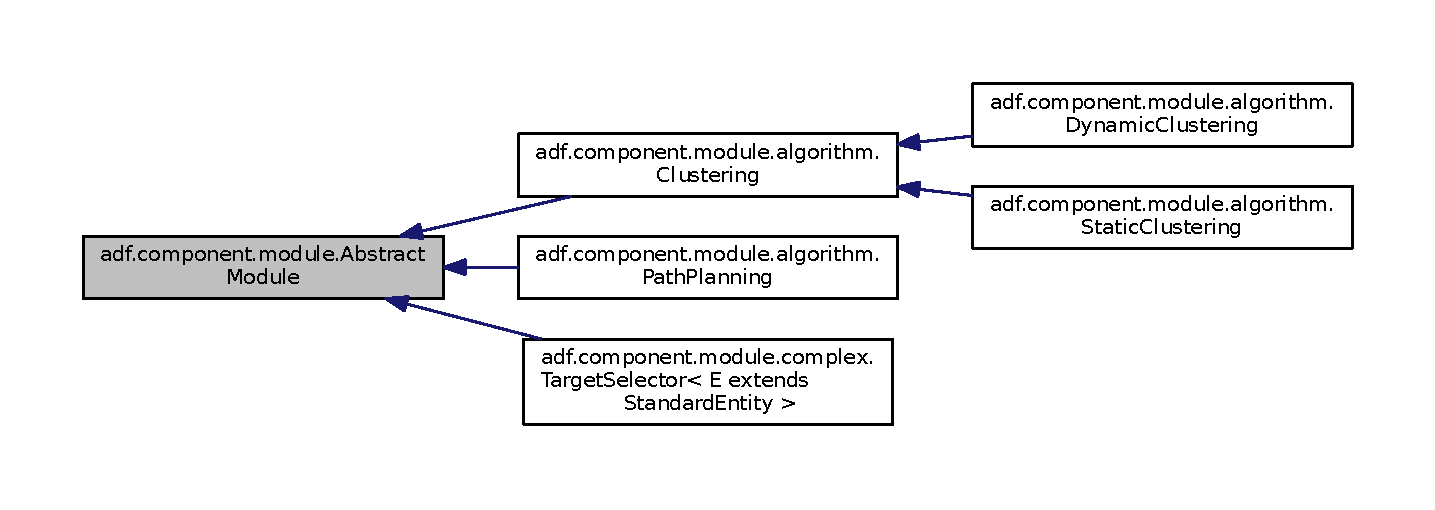
\includegraphics[width=350pt]{classadf_1_1component_1_1module_1_1AbstractModule__inherit__graph}
\end{center}
\end{figure}


adf.\+component.\+module.\+Abstract\+Module 連携図
\nopagebreak
\begin{figure}[H]
\begin{center}
\leavevmode
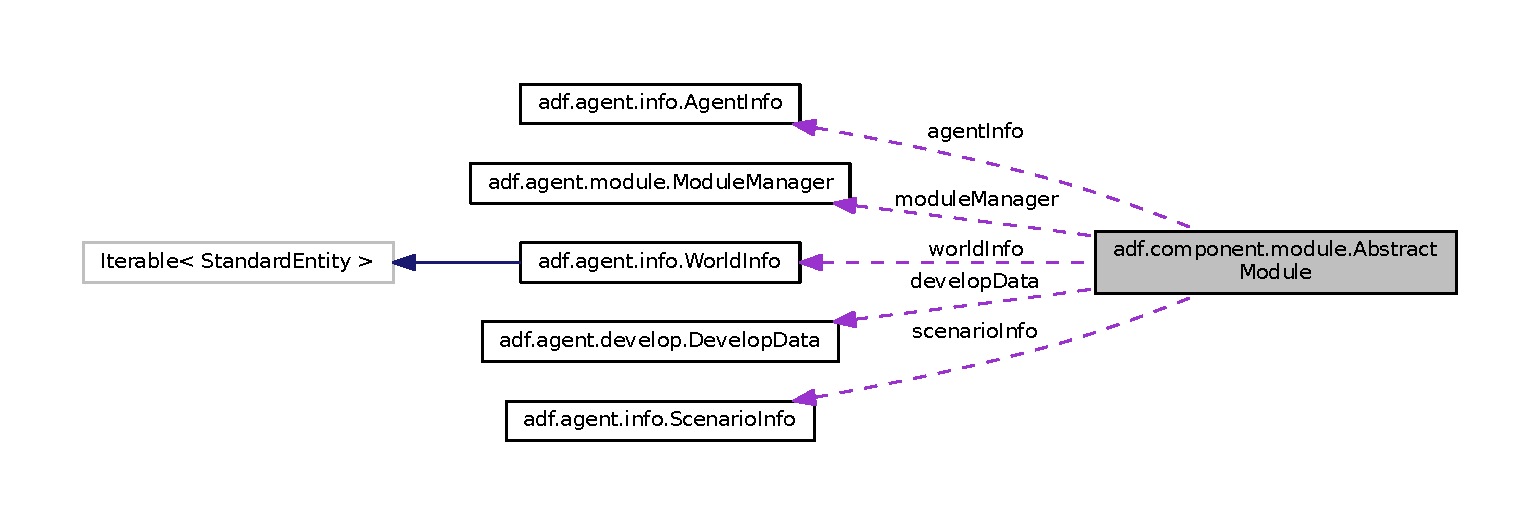
\includegraphics[width=350pt]{classadf_1_1component_1_1module_1_1AbstractModule__coll__graph}
\end{center}
\end{figure}
\subsection*{公開メンバ関数}
\begin{DoxyCompactItemize}
\item 
\hypertarget{classadf_1_1component_1_1module_1_1AbstractModule_a78b7aca7664343cd591f726b3b495e2d}{}\label{classadf_1_1component_1_1module_1_1AbstractModule_a78b7aca7664343cd591f726b3b495e2d} 
{\bfseries Abstract\+Module} (\hyperlink{classadf_1_1agent_1_1info_1_1AgentInfo}{Agent\+Info} ai, \hyperlink{classadf_1_1agent_1_1info_1_1WorldInfo}{World\+Info} wi, \hyperlink{classadf_1_1agent_1_1info_1_1ScenarioInfo}{Scenario\+Info} si, \hyperlink{classadf_1_1agent_1_1module_1_1ModuleManager}{Module\+Manager} module\+Manager, \hyperlink{classadf_1_1agent_1_1develop_1_1DevelopData}{Develop\+Data} develop\+Data)
\item 
\hypertarget{classadf_1_1component_1_1module_1_1AbstractModule_a26caa8a0a250dafb548c1a5d038597e7}{}\label{classadf_1_1component_1_1module_1_1AbstractModule_a26caa8a0a250dafb548c1a5d038597e7} 
\hyperlink{classadf_1_1component_1_1module_1_1AbstractModule}{Abstract\+Module} {\bfseries precompute} (\hyperlink{classadf_1_1agent_1_1precompute_1_1PrecomputeData}{Precompute\+Data} precompute\+Data)
\item 
\hypertarget{classadf_1_1component_1_1module_1_1AbstractModule_a2bcfc3ab4e5d5764a0cce91580fa6811}{}\label{classadf_1_1component_1_1module_1_1AbstractModule_a2bcfc3ab4e5d5764a0cce91580fa6811} 
\hyperlink{classadf_1_1component_1_1module_1_1AbstractModule}{Abstract\+Module} {\bfseries resume} (\hyperlink{classadf_1_1agent_1_1precompute_1_1PrecomputeData}{Precompute\+Data} precompute\+Data)
\item 
\hypertarget{classadf_1_1component_1_1module_1_1AbstractModule_af5c01c6d5397d0a87b556e28827b2508}{}\label{classadf_1_1component_1_1module_1_1AbstractModule_af5c01c6d5397d0a87b556e28827b2508} 
\hyperlink{classadf_1_1component_1_1module_1_1AbstractModule}{Abstract\+Module} {\bfseries preparate} ()
\item 
\hypertarget{classadf_1_1component_1_1module_1_1AbstractModule_aae6d14c3a06546d71a33d1108962cd0a}{}\label{classadf_1_1component_1_1module_1_1AbstractModule_aae6d14c3a06546d71a33d1108962cd0a} 
\hyperlink{classadf_1_1component_1_1module_1_1AbstractModule}{Abstract\+Module} {\bfseries update\+Info} (\hyperlink{classadf_1_1agent_1_1communication_1_1MessageManager}{Message\+Manager} message\+Manager)
\item 
\hypertarget{classadf_1_1component_1_1module_1_1AbstractModule_a7c70565ea94d09467dfa1f2a762de12e}{}\label{classadf_1_1component_1_1module_1_1AbstractModule_a7c70565ea94d09467dfa1f2a762de12e} 
abstract \hyperlink{classadf_1_1component_1_1module_1_1AbstractModule}{Abstract\+Module} {\bfseries calc} ()
\item 
\hypertarget{classadf_1_1component_1_1module_1_1AbstractModule_a43215e2c58e793bfe3256c8d758c12e0}{}\label{classadf_1_1component_1_1module_1_1AbstractModule_a43215e2c58e793bfe3256c8d758c12e0} 
int {\bfseries get\+Count\+Precompute} ()
\item 
\hypertarget{classadf_1_1component_1_1module_1_1AbstractModule_abe6293f6c9002eebee26041c3ed89f4f}{}\label{classadf_1_1component_1_1module_1_1AbstractModule_abe6293f6c9002eebee26041c3ed89f4f} 
int {\bfseries get\+Count\+Resume} ()
\item 
\hypertarget{classadf_1_1component_1_1module_1_1AbstractModule_a2a8f669f7dd10866c9dd687f33fd774e}{}\label{classadf_1_1component_1_1module_1_1AbstractModule_a2a8f669f7dd10866c9dd687f33fd774e} 
int {\bfseries get\+Count\+Preparate} ()
\item 
\hypertarget{classadf_1_1component_1_1module_1_1AbstractModule_a6dae9b10706502b3d2c42c967e5c7e6d}{}\label{classadf_1_1component_1_1module_1_1AbstractModule_a6dae9b10706502b3d2c42c967e5c7e6d} 
int {\bfseries get\+Count\+Update\+Info} ()
\item 
\hypertarget{classadf_1_1component_1_1module_1_1AbstractModule_ab7b898f0a858929ea6505e173a50290b}{}\label{classadf_1_1component_1_1module_1_1AbstractModule_ab7b898f0a858929ea6505e173a50290b} 
void {\bfseries reset\+Count\+Precompute} ()
\item 
\hypertarget{classadf_1_1component_1_1module_1_1AbstractModule_a6760931b28553d4ec3ea7de32c7d7eff}{}\label{classadf_1_1component_1_1module_1_1AbstractModule_a6760931b28553d4ec3ea7de32c7d7eff} 
void {\bfseries reset\+Count\+Resume} ()
\item 
\hypertarget{classadf_1_1component_1_1module_1_1AbstractModule_a4280fac9e8491096101e8ec3d4f4a497}{}\label{classadf_1_1component_1_1module_1_1AbstractModule_a4280fac9e8491096101e8ec3d4f4a497} 
void {\bfseries reset\+Count\+Preparate} ()
\item 
\hypertarget{classadf_1_1component_1_1module_1_1AbstractModule_ae0892cca705ee00cfc91106ea2d222fd}{}\label{classadf_1_1component_1_1module_1_1AbstractModule_ae0892cca705ee00cfc91106ea2d222fd} 
void {\bfseries reset\+Count\+Update\+Info} ()
\end{DoxyCompactItemize}
\subsection*{限定公開変数類}
\begin{DoxyCompactItemize}
\item 
\hypertarget{classadf_1_1component_1_1module_1_1AbstractModule_a4f3c28aad990c2d969f06f0cd7955281}{}\label{classadf_1_1component_1_1module_1_1AbstractModule_a4f3c28aad990c2d969f06f0cd7955281} 
\hyperlink{classadf_1_1agent_1_1info_1_1ScenarioInfo}{Scenario\+Info} {\bfseries scenario\+Info}
\item 
\hypertarget{classadf_1_1component_1_1module_1_1AbstractModule_a7899d34c90df44723cdcb35653735a54}{}\label{classadf_1_1component_1_1module_1_1AbstractModule_a7899d34c90df44723cdcb35653735a54} 
\hyperlink{classadf_1_1agent_1_1info_1_1AgentInfo}{Agent\+Info} {\bfseries agent\+Info}
\item 
\hypertarget{classadf_1_1component_1_1module_1_1AbstractModule_a55634f32bad39f01c25258278fbc37aa}{}\label{classadf_1_1component_1_1module_1_1AbstractModule_a55634f32bad39f01c25258278fbc37aa} 
\hyperlink{classadf_1_1agent_1_1info_1_1WorldInfo}{World\+Info} {\bfseries world\+Info}
\item 
\hypertarget{classadf_1_1component_1_1module_1_1AbstractModule_a4e44edcd327e67f929c357b77b127f89}{}\label{classadf_1_1component_1_1module_1_1AbstractModule_a4e44edcd327e67f929c357b77b127f89} 
\hyperlink{classadf_1_1agent_1_1module_1_1ModuleManager}{Module\+Manager} {\bfseries module\+Manager}
\item 
\hypertarget{classadf_1_1component_1_1module_1_1AbstractModule_aa7337d08e34428dfc5baa9582c3d4444}{}\label{classadf_1_1component_1_1module_1_1AbstractModule_aa7337d08e34428dfc5baa9582c3d4444} 
\hyperlink{classadf_1_1agent_1_1develop_1_1DevelopData}{Develop\+Data} {\bfseries develop\+Data}
\end{DoxyCompactItemize}


このクラス詳解は次のファイルから抽出されました\+:\begin{DoxyCompactItemize}
\item 
src/main/java/adf/component/module/Abstract\+Module.\+java\end{DoxyCompactItemize}

\hypertarget{classadf_1_1agent_1_1action_1_1Action}{}\section{adf.\+agent.\+action.\+Action Class Reference}
\label{classadf_1_1agent_1_1action_1_1Action}\index{adf.\+agent.\+action.\+Action@{adf.\+agent.\+action.\+Action}}


Inheritance diagram for adf.\+agent.\+action.\+Action\+:
\nopagebreak
\begin{figure}[H]
\begin{center}
\leavevmode
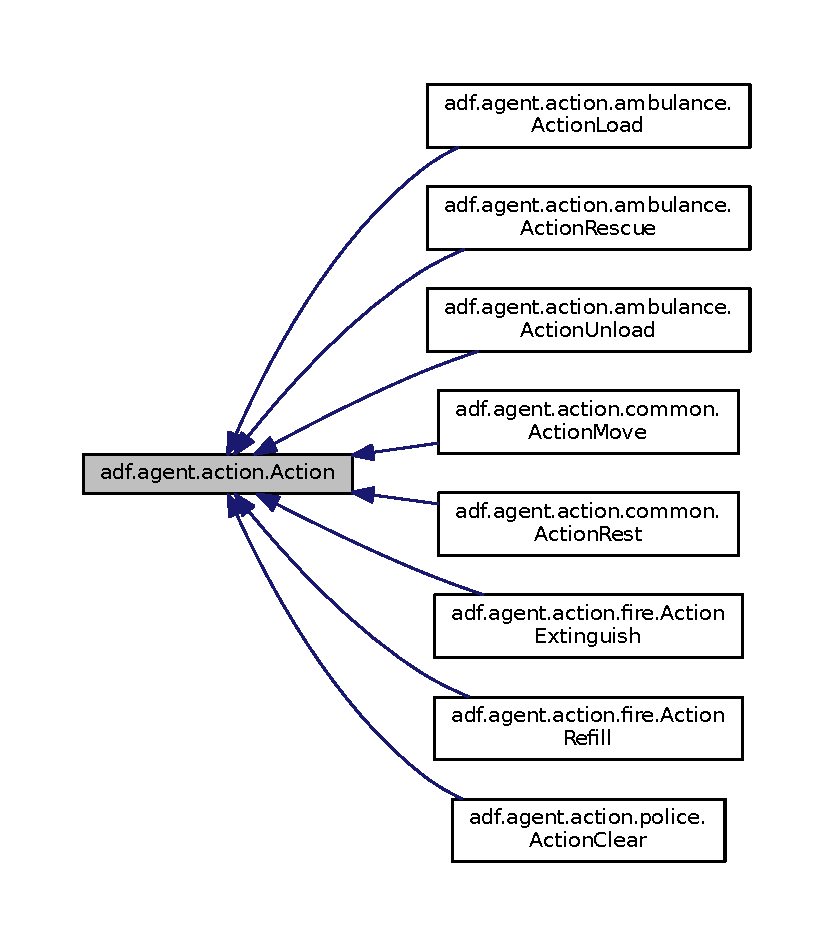
\includegraphics[width=350pt]{classadf_1_1agent_1_1action_1_1Action__inherit__graph}
\end{center}
\end{figure}
\subsection*{Public Member Functions}
\begin{DoxyCompactItemize}
\item 
\hypertarget{classadf_1_1agent_1_1action_1_1Action_afc2cef4d52ee76566ee518bab9d5f145}{}\label{classadf_1_1agent_1_1action_1_1Action_afc2cef4d52ee76566ee518bab9d5f145} 
abstract Message {\bfseries get\+Command} (Entity\+ID agent\+ID, int time)
\end{DoxyCompactItemize}


The documentation for this class was generated from the following file\+:\begin{DoxyCompactItemize}
\item 
src/main/java/adf/agent/action/Action.\+java\end{DoxyCompactItemize}

\hypertarget{classadf_1_1agent_1_1action_1_1police_1_1ActionClear}{}\section{adf.\+agent.\+action.\+police.\+Action\+Clear クラス}
\label{classadf_1_1agent_1_1action_1_1police_1_1ActionClear}\index{adf.\+agent.\+action.\+police.\+Action\+Clear@{adf.\+agent.\+action.\+police.\+Action\+Clear}}


adf.\+agent.\+action.\+police.\+Action\+Clear の継承関係図
\nopagebreak
\begin{figure}[H]
\begin{center}
\leavevmode
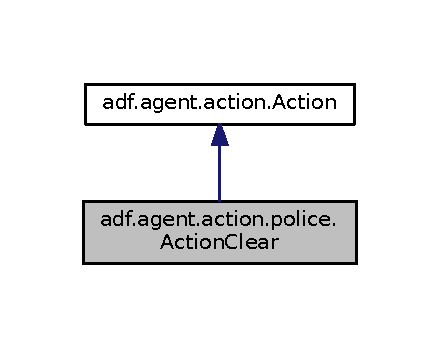
\includegraphics[width=211pt]{classadf_1_1agent_1_1action_1_1police_1_1ActionClear__inherit__graph}
\end{center}
\end{figure}


adf.\+agent.\+action.\+police.\+Action\+Clear 連携図
\nopagebreak
\begin{figure}[H]
\begin{center}
\leavevmode
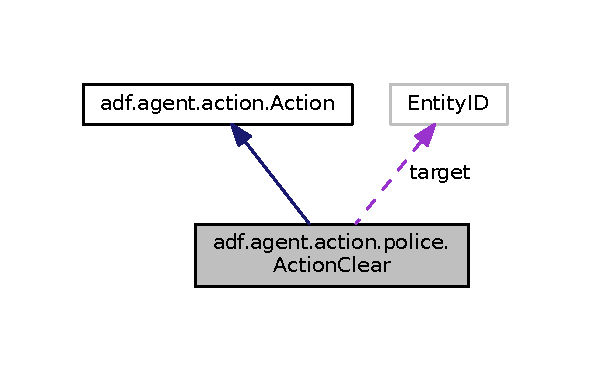
\includegraphics[width=284pt]{classadf_1_1agent_1_1action_1_1police_1_1ActionClear__coll__graph}
\end{center}
\end{figure}
\subsection*{公開メンバ関数}
\begin{DoxyCompactItemize}
\item 
\hypertarget{classadf_1_1agent_1_1action_1_1police_1_1ActionClear_a3bd9423c88033d9f96681790c1df76c8}{}\label{classadf_1_1agent_1_1action_1_1police_1_1ActionClear_a3bd9423c88033d9f96681790c1df76c8} 
{\bfseries Action\+Clear} (Entity\+ID target\+ID)
\item 
\hypertarget{classadf_1_1agent_1_1action_1_1police_1_1ActionClear_a0e278fa4eb4caed02ac8849f4d457ca4}{}\label{classadf_1_1agent_1_1action_1_1police_1_1ActionClear_a0e278fa4eb4caed02ac8849f4d457ca4} 
{\bfseries Action\+Clear} (Blockade blockade)
\item 
\hypertarget{classadf_1_1agent_1_1action_1_1police_1_1ActionClear_aefd49775f6b6747b1348ca19e0c2180b}{}\label{classadf_1_1agent_1_1action_1_1police_1_1ActionClear_aefd49775f6b6747b1348ca19e0c2180b} 
{\bfseries Action\+Clear} (\hyperlink{classadf_1_1agent_1_1info_1_1AgentInfo}{Agent\+Info} agent, Vector2D vector)
\item 
\hypertarget{classadf_1_1agent_1_1action_1_1police_1_1ActionClear_ab0cc726000493ae407f0d36836cdebdd}{}\label{classadf_1_1agent_1_1action_1_1police_1_1ActionClear_ab0cc726000493ae407f0d36836cdebdd} 
{\bfseries Action\+Clear} (int destX, int destY)
\item 
\hypertarget{classadf_1_1agent_1_1action_1_1police_1_1ActionClear_aa32a3ea0f7f4799c43b2e1800b7ff9dc}{}\label{classadf_1_1agent_1_1action_1_1police_1_1ActionClear_aa32a3ea0f7f4799c43b2e1800b7ff9dc} 
{\bfseries Action\+Clear} (int destX, int destY, Blockade blockade)
\item 
\hypertarget{classadf_1_1agent_1_1action_1_1police_1_1ActionClear_ab293584ac1c01b11d1fbb21cc57e0e4c}{}\label{classadf_1_1agent_1_1action_1_1police_1_1ActionClear_ab293584ac1c01b11d1fbb21cc57e0e4c} 
String {\bfseries to\+String} ()
\item 
\hypertarget{classadf_1_1agent_1_1action_1_1police_1_1ActionClear_a63b59f8379ad2c4889701b5ef62312a3}{}\label{classadf_1_1agent_1_1action_1_1police_1_1ActionClear_a63b59f8379ad2c4889701b5ef62312a3} 
boolean {\bfseries get\+Use\+Old\+Function} ()
\item 
\hypertarget{classadf_1_1agent_1_1action_1_1police_1_1ActionClear_a48b13863cf0791be4a75762ddac979b5}{}\label{classadf_1_1agent_1_1action_1_1police_1_1ActionClear_a48b13863cf0791be4a75762ddac979b5} 
Entity\+ID {\bfseries get\+Target} ()
\item 
\hypertarget{classadf_1_1agent_1_1action_1_1police_1_1ActionClear_a21e54fc3a4289d546398f8f623ffe52e}{}\label{classadf_1_1agent_1_1action_1_1police_1_1ActionClear_a21e54fc3a4289d546398f8f623ffe52e} 
int {\bfseries get\+PosX} ()
\item 
\hypertarget{classadf_1_1agent_1_1action_1_1police_1_1ActionClear_a0b81ff28273e1c267147e58cf4bf6595}{}\label{classadf_1_1agent_1_1action_1_1police_1_1ActionClear_a0b81ff28273e1c267147e58cf4bf6595} 
int {\bfseries get\+PosY} ()
\item 
\hypertarget{classadf_1_1agent_1_1action_1_1police_1_1ActionClear_add96a279d2f46903fb7419be6ff21cca}{}\label{classadf_1_1agent_1_1action_1_1police_1_1ActionClear_add96a279d2f46903fb7419be6ff21cca} 
Message {\bfseries get\+Command} (Entity\+ID agent\+ID, int time)
\end{DoxyCompactItemize}
\subsection*{限定公開変数類}
\begin{DoxyCompactItemize}
\item 
\hypertarget{classadf_1_1agent_1_1action_1_1police_1_1ActionClear_a5623b17139cc8f34bbd1f22f22bf836d}{}\label{classadf_1_1agent_1_1action_1_1police_1_1ActionClear_a5623b17139cc8f34bbd1f22f22bf836d} 
Entity\+ID {\bfseries target}
\end{DoxyCompactItemize}


このクラス詳解は次のファイルから抽出されました\+:\begin{DoxyCompactItemize}
\item 
src/main/java/adf/agent/action/police/Action\+Clear.\+java\end{DoxyCompactItemize}

\hypertarget{classadf_1_1agent_1_1action_1_1fire_1_1ActionExtinguish}{}\section{adf.\+agent.\+action.\+fire.\+Action\+Extinguish Class Reference}
\label{classadf_1_1agent_1_1action_1_1fire_1_1ActionExtinguish}\index{adf.\+agent.\+action.\+fire.\+Action\+Extinguish@{adf.\+agent.\+action.\+fire.\+Action\+Extinguish}}


Inheritance diagram for adf.\+agent.\+action.\+fire.\+Action\+Extinguish\+:
\nopagebreak
\begin{figure}[H]
\begin{center}
\leavevmode
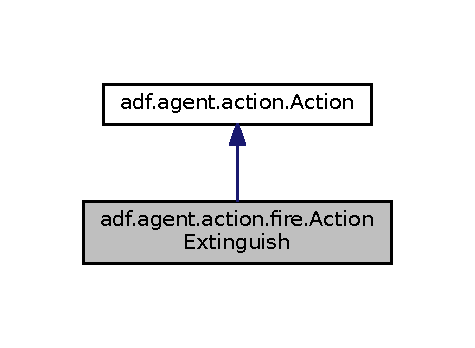
\includegraphics[width=228pt]{classadf_1_1agent_1_1action_1_1fire_1_1ActionExtinguish__inherit__graph}
\end{center}
\end{figure}


Collaboration diagram for adf.\+agent.\+action.\+fire.\+Action\+Extinguish\+:
\nopagebreak
\begin{figure}[H]
\begin{center}
\leavevmode
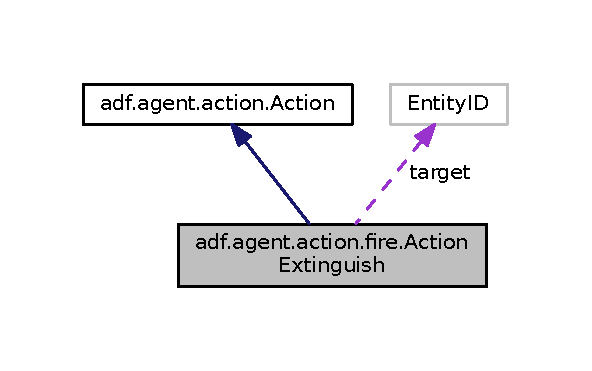
\includegraphics[width=284pt]{classadf_1_1agent_1_1action_1_1fire_1_1ActionExtinguish__coll__graph}
\end{center}
\end{figure}
\subsection*{Public Member Functions}
\begin{DoxyCompactItemize}
\item 
\hypertarget{classadf_1_1agent_1_1action_1_1fire_1_1ActionExtinguish_a71b5feb48519721e31eb8d8b9ec24b56}{}\label{classadf_1_1agent_1_1action_1_1fire_1_1ActionExtinguish_a71b5feb48519721e31eb8d8b9ec24b56} 
{\bfseries Action\+Extinguish} (Entity\+ID target\+ID, int max\+Power)
\item 
\hypertarget{classadf_1_1agent_1_1action_1_1fire_1_1ActionExtinguish_a9bb366ec06f181b38dd161d24f32ab6c}{}\label{classadf_1_1agent_1_1action_1_1fire_1_1ActionExtinguish_a9bb366ec06f181b38dd161d24f32ab6c} 
{\bfseries Action\+Extinguish} (Building building, int max\+Power)
\item 
\hypertarget{classadf_1_1agent_1_1action_1_1fire_1_1ActionExtinguish_a409f07138feced350503502b98075b8f}{}\label{classadf_1_1agent_1_1action_1_1fire_1_1ActionExtinguish_a409f07138feced350503502b98075b8f} 
String {\bfseries to\+String} ()
\item 
\hypertarget{classadf_1_1agent_1_1action_1_1fire_1_1ActionExtinguish_a300cc94f9d9af74310dcc86ff5a254a4}{}\label{classadf_1_1agent_1_1action_1_1fire_1_1ActionExtinguish_a300cc94f9d9af74310dcc86ff5a254a4} 
int {\bfseries get\+Power} ()
\item 
\hypertarget{classadf_1_1agent_1_1action_1_1fire_1_1ActionExtinguish_af47ac8ae164313f7ce8ee7035e2095b0}{}\label{classadf_1_1agent_1_1action_1_1fire_1_1ActionExtinguish_af47ac8ae164313f7ce8ee7035e2095b0} 
Entity\+ID {\bfseries get\+Target} ()
\item 
\hypertarget{classadf_1_1agent_1_1action_1_1fire_1_1ActionExtinguish_a4aea8c37d2298767efb3c05c63414960}{}\label{classadf_1_1agent_1_1action_1_1fire_1_1ActionExtinguish_a4aea8c37d2298767efb3c05c63414960} 
Message {\bfseries get\+Command} (Entity\+ID agent\+ID, int time)
\end{DoxyCompactItemize}
\subsection*{Protected Attributes}
\begin{DoxyCompactItemize}
\item 
\hypertarget{classadf_1_1agent_1_1action_1_1fire_1_1ActionExtinguish_af2154ee8ad5aac2e8dea5e13d70432f2}{}\label{classadf_1_1agent_1_1action_1_1fire_1_1ActionExtinguish_af2154ee8ad5aac2e8dea5e13d70432f2} 
Entity\+ID {\bfseries target}
\end{DoxyCompactItemize}


The documentation for this class was generated from the following file\+:\begin{DoxyCompactItemize}
\item 
src/main/java/adf/agent/action/fire/Action\+Extinguish.\+java\end{DoxyCompactItemize}

\hypertarget{classadf_1_1agent_1_1action_1_1ambulance_1_1ActionLoad}{}\section{adf.\+agent.\+action.\+ambulance.\+Action\+Load Class Reference}
\label{classadf_1_1agent_1_1action_1_1ambulance_1_1ActionLoad}\index{adf.\+agent.\+action.\+ambulance.\+Action\+Load@{adf.\+agent.\+action.\+ambulance.\+Action\+Load}}


Inheritance diagram for adf.\+agent.\+action.\+ambulance.\+Action\+Load\+:
\nopagebreak
\begin{figure}[H]
\begin{center}
\leavevmode
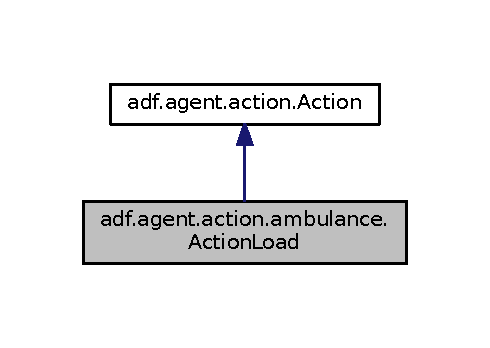
\includegraphics[width=235pt]{classadf_1_1agent_1_1action_1_1ambulance_1_1ActionLoad__inherit__graph}
\end{center}
\end{figure}


Collaboration diagram for adf.\+agent.\+action.\+ambulance.\+Action\+Load\+:
\nopagebreak
\begin{figure}[H]
\begin{center}
\leavevmode
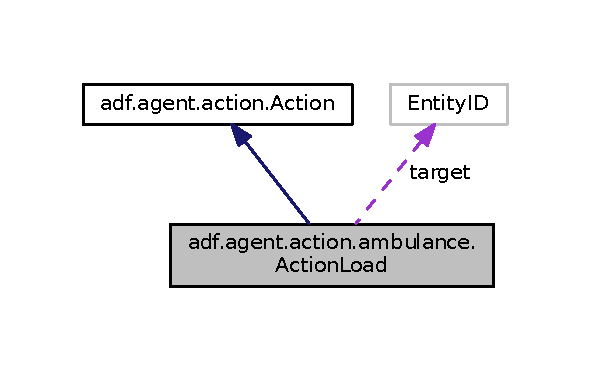
\includegraphics[width=284pt]{classadf_1_1agent_1_1action_1_1ambulance_1_1ActionLoad__coll__graph}
\end{center}
\end{figure}
\subsection*{Public Member Functions}
\begin{DoxyCompactItemize}
\item 
\hypertarget{classadf_1_1agent_1_1action_1_1ambulance_1_1ActionLoad_afb8c917e4bdfcef0e6083e3c89709aa7}{}\label{classadf_1_1agent_1_1action_1_1ambulance_1_1ActionLoad_afb8c917e4bdfcef0e6083e3c89709aa7} 
{\bfseries Action\+Load} (Entity\+ID target\+ID)
\item 
\hypertarget{classadf_1_1agent_1_1action_1_1ambulance_1_1ActionLoad_a5dedd5ce60d85b8dfc1ed698b59f9927}{}\label{classadf_1_1agent_1_1action_1_1ambulance_1_1ActionLoad_a5dedd5ce60d85b8dfc1ed698b59f9927} 
{\bfseries Action\+Load} (Civilian civilian)
\item 
\hypertarget{classadf_1_1agent_1_1action_1_1ambulance_1_1ActionLoad_abef023f9c55eced92f5c1f6b99cd76a1}{}\label{classadf_1_1agent_1_1action_1_1ambulance_1_1ActionLoad_abef023f9c55eced92f5c1f6b99cd76a1} 
String {\bfseries to\+String} ()
\item 
\hypertarget{classadf_1_1agent_1_1action_1_1ambulance_1_1ActionLoad_a01c6dcdb32d5b04b355a52c74fcab728}{}\label{classadf_1_1agent_1_1action_1_1ambulance_1_1ActionLoad_a01c6dcdb32d5b04b355a52c74fcab728} 
Entity\+ID {\bfseries get\+Target} ()
\item 
\hypertarget{classadf_1_1agent_1_1action_1_1ambulance_1_1ActionLoad_a28c77b2dc4e23671af98d958c39988c9}{}\label{classadf_1_1agent_1_1action_1_1ambulance_1_1ActionLoad_a28c77b2dc4e23671af98d958c39988c9} 
Message {\bfseries get\+Command} (Entity\+ID agent\+ID, int time)
\end{DoxyCompactItemize}
\subsection*{Protected Attributes}
\begin{DoxyCompactItemize}
\item 
\hypertarget{classadf_1_1agent_1_1action_1_1ambulance_1_1ActionLoad_a6146d26a2100734e0794bc4dfa408a24}{}\label{classadf_1_1agent_1_1action_1_1ambulance_1_1ActionLoad_a6146d26a2100734e0794bc4dfa408a24} 
Entity\+ID {\bfseries target}
\end{DoxyCompactItemize}


The documentation for this class was generated from the following file\+:\begin{DoxyCompactItemize}
\item 
src/main/java/adf/agent/action/ambulance/Action\+Load.\+java\end{DoxyCompactItemize}

\hypertarget{classadf_1_1agent_1_1action_1_1common_1_1ActionMove}{}\section{adf.\+agent.\+action.\+common.\+Action\+Move Class Reference}
\label{classadf_1_1agent_1_1action_1_1common_1_1ActionMove}\index{adf.\+agent.\+action.\+common.\+Action\+Move@{adf.\+agent.\+action.\+common.\+Action\+Move}}


Inheritance diagram for adf.\+agent.\+action.\+common.\+Action\+Move\+:
\nopagebreak
\begin{figure}[H]
\begin{center}
\leavevmode
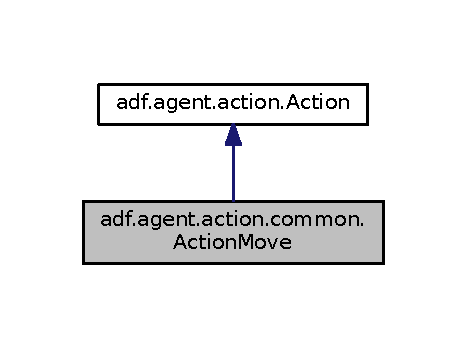
\includegraphics[width=224pt]{classadf_1_1agent_1_1action_1_1common_1_1ActionMove__inherit__graph}
\end{center}
\end{figure}


Collaboration diagram for adf.\+agent.\+action.\+common.\+Action\+Move\+:
\nopagebreak
\begin{figure}[H]
\begin{center}
\leavevmode
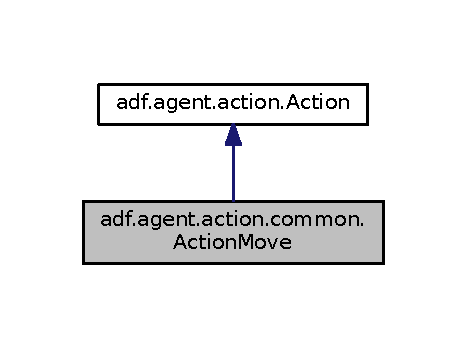
\includegraphics[width=224pt]{classadf_1_1agent_1_1action_1_1common_1_1ActionMove__coll__graph}
\end{center}
\end{figure}
\subsection*{Public Member Functions}
\begin{DoxyCompactItemize}
\item 
\hypertarget{classadf_1_1agent_1_1action_1_1common_1_1ActionMove_a446fb0a7f2d7ac5def8ccb4915e84443}{}\label{classadf_1_1agent_1_1action_1_1common_1_1ActionMove_a446fb0a7f2d7ac5def8ccb4915e84443} 
{\bfseries Action\+Move} (List$<$ Entity\+ID $>$ move\+Path)
\item 
\hypertarget{classadf_1_1agent_1_1action_1_1common_1_1ActionMove_aedc59794067e863a2881b623024f36eb}{}\label{classadf_1_1agent_1_1action_1_1common_1_1ActionMove_aedc59794067e863a2881b623024f36eb} 
{\bfseries Action\+Move} (List$<$ Entity\+ID $>$ move\+Path, int destinationX, int destinationY)
\item 
\hypertarget{classadf_1_1agent_1_1action_1_1common_1_1ActionMove_a73a448873ec5ef05f94369b7a0091183}{}\label{classadf_1_1agent_1_1action_1_1common_1_1ActionMove_a73a448873ec5ef05f94369b7a0091183} 
String {\bfseries to\+String} ()
\item 
\hypertarget{classadf_1_1agent_1_1action_1_1common_1_1ActionMove_a079ea88ac540e4c274d8590700843ed5}{}\label{classadf_1_1agent_1_1action_1_1common_1_1ActionMove_a079ea88ac540e4c274d8590700843ed5} 
List$<$ Entity\+ID $>$ {\bfseries get\+Path} ()
\item 
\hypertarget{classadf_1_1agent_1_1action_1_1common_1_1ActionMove_aaddb1fd9d8724f78dc645a534647de35}{}\label{classadf_1_1agent_1_1action_1_1common_1_1ActionMove_aaddb1fd9d8724f78dc645a534647de35} 
boolean {\bfseries get\+Use\+Position} ()
\item 
\hypertarget{classadf_1_1agent_1_1action_1_1common_1_1ActionMove_ab46a8688e7a400327e0709b5747227a3}{}\label{classadf_1_1agent_1_1action_1_1common_1_1ActionMove_ab46a8688e7a400327e0709b5747227a3} 
int {\bfseries get\+PosX} ()
\item 
\hypertarget{classadf_1_1agent_1_1action_1_1common_1_1ActionMove_a1e8adba10aa1ee1212e9be9e9a8fb4f8}{}\label{classadf_1_1agent_1_1action_1_1common_1_1ActionMove_a1e8adba10aa1ee1212e9be9e9a8fb4f8} 
int {\bfseries get\+PosY} ()
\item 
\hypertarget{classadf_1_1agent_1_1action_1_1common_1_1ActionMove_a0c0647b59ef2030d756dd8023acabf17}{}\label{classadf_1_1agent_1_1action_1_1common_1_1ActionMove_a0c0647b59ef2030d756dd8023acabf17} 
Message {\bfseries get\+Command} (Entity\+ID agent\+ID, int time)
\end{DoxyCompactItemize}


The documentation for this class was generated from the following file\+:\begin{DoxyCompactItemize}
\item 
src/main/java/adf/agent/action/common/Action\+Move.\+java\end{DoxyCompactItemize}

\hypertarget{classadf_1_1agent_1_1action_1_1fire_1_1ActionRefill}{}\section{adf.\+agent.\+action.\+fire.\+Action\+Refill Class Reference}
\label{classadf_1_1agent_1_1action_1_1fire_1_1ActionRefill}\index{adf.\+agent.\+action.\+fire.\+Action\+Refill@{adf.\+agent.\+action.\+fire.\+Action\+Refill}}


Inheritance diagram for adf.\+agent.\+action.\+fire.\+Action\+Refill\+:
\nopagebreak
\begin{figure}[H]
\begin{center}
\leavevmode
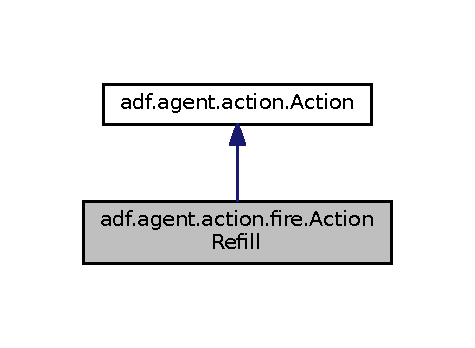
\includegraphics[width=228pt]{classadf_1_1agent_1_1action_1_1fire_1_1ActionRefill__inherit__graph}
\end{center}
\end{figure}


Collaboration diagram for adf.\+agent.\+action.\+fire.\+Action\+Refill\+:
\nopagebreak
\begin{figure}[H]
\begin{center}
\leavevmode
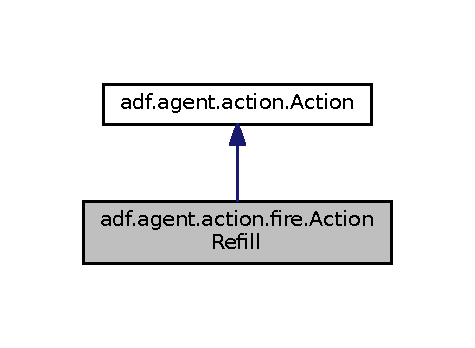
\includegraphics[width=228pt]{classadf_1_1agent_1_1action_1_1fire_1_1ActionRefill__coll__graph}
\end{center}
\end{figure}
\subsection*{Public Member Functions}
\begin{DoxyCompactItemize}
\item 
\hypertarget{classadf_1_1agent_1_1action_1_1fire_1_1ActionRefill_aefdc3e931e79ebc71cd29bdcad939109}{}\label{classadf_1_1agent_1_1action_1_1fire_1_1ActionRefill_aefdc3e931e79ebc71cd29bdcad939109} 
String {\bfseries to\+String} ()
\item 
\hypertarget{classadf_1_1agent_1_1action_1_1fire_1_1ActionRefill_a2bed6b1eb1ece6d45e6b1526b69b337a}{}\label{classadf_1_1agent_1_1action_1_1fire_1_1ActionRefill_a2bed6b1eb1ece6d45e6b1526b69b337a} 
Message {\bfseries get\+Command} (Entity\+ID agent\+ID, int time)
\end{DoxyCompactItemize}


The documentation for this class was generated from the following file\+:\begin{DoxyCompactItemize}
\item 
src/main/java/adf/agent/action/fire/Action\+Refill.\+java\end{DoxyCompactItemize}

\hypertarget{classadf_1_1agent_1_1action_1_1ambulance_1_1ActionRescue}{}\section{adf.\+agent.\+action.\+ambulance.\+Action\+Rescue Class Reference}
\label{classadf_1_1agent_1_1action_1_1ambulance_1_1ActionRescue}\index{adf.\+agent.\+action.\+ambulance.\+Action\+Rescue@{adf.\+agent.\+action.\+ambulance.\+Action\+Rescue}}


Inheritance diagram for adf.\+agent.\+action.\+ambulance.\+Action\+Rescue\+:
\nopagebreak
\begin{figure}[H]
\begin{center}
\leavevmode
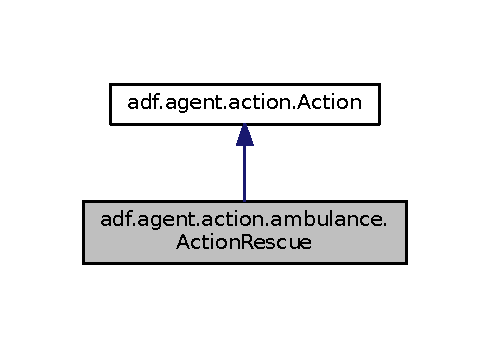
\includegraphics[width=235pt]{classadf_1_1agent_1_1action_1_1ambulance_1_1ActionRescue__inherit__graph}
\end{center}
\end{figure}


Collaboration diagram for adf.\+agent.\+action.\+ambulance.\+Action\+Rescue\+:
\nopagebreak
\begin{figure}[H]
\begin{center}
\leavevmode
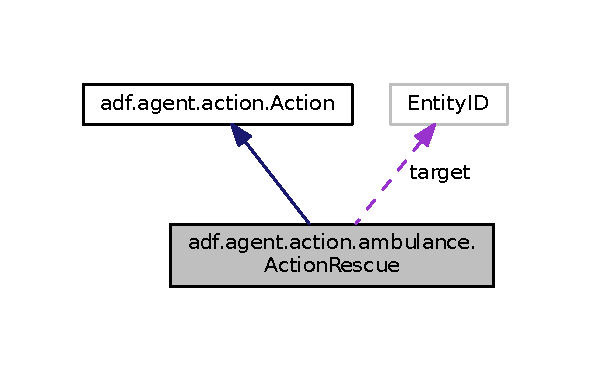
\includegraphics[width=284pt]{classadf_1_1agent_1_1action_1_1ambulance_1_1ActionRescue__coll__graph}
\end{center}
\end{figure}
\subsection*{Public Member Functions}
\begin{DoxyCompactItemize}
\item 
\hypertarget{classadf_1_1agent_1_1action_1_1ambulance_1_1ActionRescue_a775f329369155fafbacbfe011205a028}{}\label{classadf_1_1agent_1_1action_1_1ambulance_1_1ActionRescue_a775f329369155fafbacbfe011205a028} 
{\bfseries Action\+Rescue} (Entity\+ID target\+ID)
\item 
\hypertarget{classadf_1_1agent_1_1action_1_1ambulance_1_1ActionRescue_a31dc4b96abd6a526b0942971814efb75}{}\label{classadf_1_1agent_1_1action_1_1ambulance_1_1ActionRescue_a31dc4b96abd6a526b0942971814efb75} 
{\bfseries Action\+Rescue} (Human human)
\item 
\hypertarget{classadf_1_1agent_1_1action_1_1ambulance_1_1ActionRescue_a5543738527ed1ac96dee4c3248c9edca}{}\label{classadf_1_1agent_1_1action_1_1ambulance_1_1ActionRescue_a5543738527ed1ac96dee4c3248c9edca} 
String {\bfseries to\+String} ()
\item 
\hypertarget{classadf_1_1agent_1_1action_1_1ambulance_1_1ActionRescue_a526187da7c7b537cd8ec6f297b3a66e0}{}\label{classadf_1_1agent_1_1action_1_1ambulance_1_1ActionRescue_a526187da7c7b537cd8ec6f297b3a66e0} 
Entity\+ID {\bfseries get\+Target} ()
\item 
\hypertarget{classadf_1_1agent_1_1action_1_1ambulance_1_1ActionRescue_a74d4a3b6d9a649e96ec40cf323d1e416}{}\label{classadf_1_1agent_1_1action_1_1ambulance_1_1ActionRescue_a74d4a3b6d9a649e96ec40cf323d1e416} 
Message {\bfseries get\+Command} (Entity\+ID agent\+ID, int time)
\end{DoxyCompactItemize}
\subsection*{Protected Attributes}
\begin{DoxyCompactItemize}
\item 
\hypertarget{classadf_1_1agent_1_1action_1_1ambulance_1_1ActionRescue_a4280350fbfd1d62e5bc45affcebfe701}{}\label{classadf_1_1agent_1_1action_1_1ambulance_1_1ActionRescue_a4280350fbfd1d62e5bc45affcebfe701} 
Entity\+ID {\bfseries target}
\end{DoxyCompactItemize}


The documentation for this class was generated from the following file\+:\begin{DoxyCompactItemize}
\item 
src/main/java/adf/agent/action/ambulance/Action\+Rescue.\+java\end{DoxyCompactItemize}

\hypertarget{classadf_1_1agent_1_1action_1_1common_1_1ActionRest}{}\section{adf.\+agent.\+action.\+common.\+Action\+Rest クラス}
\label{classadf_1_1agent_1_1action_1_1common_1_1ActionRest}\index{adf.\+agent.\+action.\+common.\+Action\+Rest@{adf.\+agent.\+action.\+common.\+Action\+Rest}}


adf.\+agent.\+action.\+common.\+Action\+Rest の継承関係図
\nopagebreak
\begin{figure}[H]
\begin{center}
\leavevmode
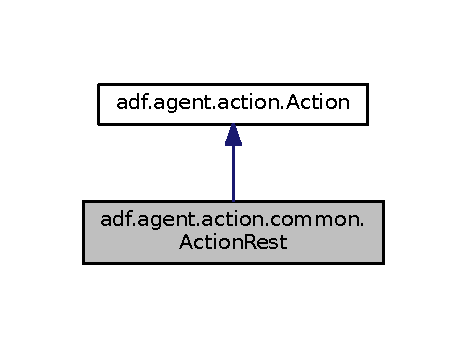
\includegraphics[width=224pt]{classadf_1_1agent_1_1action_1_1common_1_1ActionRest__inherit__graph}
\end{center}
\end{figure}


adf.\+agent.\+action.\+common.\+Action\+Rest 連携図
\nopagebreak
\begin{figure}[H]
\begin{center}
\leavevmode
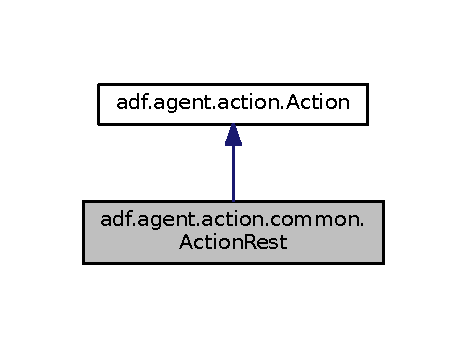
\includegraphics[width=224pt]{classadf_1_1agent_1_1action_1_1common_1_1ActionRest__coll__graph}
\end{center}
\end{figure}
\subsection*{公開メンバ関数}
\begin{DoxyCompactItemize}
\item 
\hypertarget{classadf_1_1agent_1_1action_1_1common_1_1ActionRest_a739ba879f9ae9da9a46db83914026ff4}{}\label{classadf_1_1agent_1_1action_1_1common_1_1ActionRest_a739ba879f9ae9da9a46db83914026ff4} 
String {\bfseries to\+String} ()
\item 
\hypertarget{classadf_1_1agent_1_1action_1_1common_1_1ActionRest_a48270767d6992f55bd6184e942a6436b}{}\label{classadf_1_1agent_1_1action_1_1common_1_1ActionRest_a48270767d6992f55bd6184e942a6436b} 
Message {\bfseries get\+Command} (Entity\+ID agent\+ID, int time)
\end{DoxyCompactItemize}


このクラス詳解は次のファイルから抽出されました\+:\begin{DoxyCompactItemize}
\item 
src/main/java/adf/agent/action/common/Action\+Rest.\+java\end{DoxyCompactItemize}

\hypertarget{classadf_1_1agent_1_1action_1_1ambulance_1_1ActionUnload}{}\section{adf.\+agent.\+action.\+ambulance.\+Action\+Unload クラス}
\label{classadf_1_1agent_1_1action_1_1ambulance_1_1ActionUnload}\index{adf.\+agent.\+action.\+ambulance.\+Action\+Unload@{adf.\+agent.\+action.\+ambulance.\+Action\+Unload}}


adf.\+agent.\+action.\+ambulance.\+Action\+Unload の継承関係図
\nopagebreak
\begin{figure}[H]
\begin{center}
\leavevmode
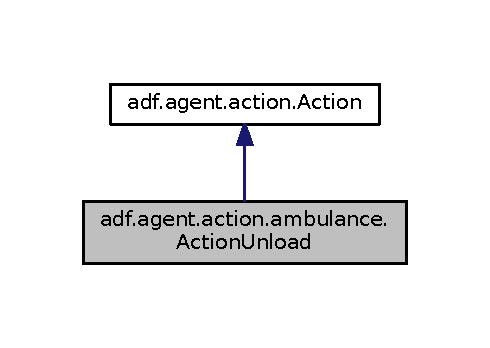
\includegraphics[width=235pt]{classadf_1_1agent_1_1action_1_1ambulance_1_1ActionUnload__inherit__graph}
\end{center}
\end{figure}


adf.\+agent.\+action.\+ambulance.\+Action\+Unload 連携図
\nopagebreak
\begin{figure}[H]
\begin{center}
\leavevmode
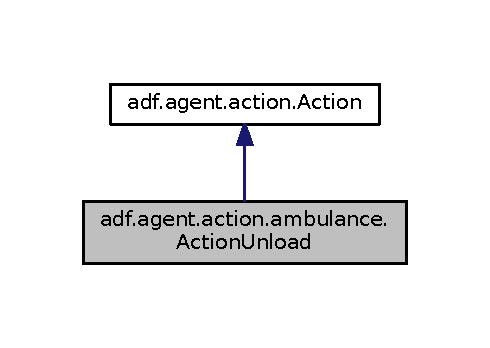
\includegraphics[width=235pt]{classadf_1_1agent_1_1action_1_1ambulance_1_1ActionUnload__coll__graph}
\end{center}
\end{figure}
\subsection*{公開メンバ関数}
\begin{DoxyCompactItemize}
\item 
\hypertarget{classadf_1_1agent_1_1action_1_1ambulance_1_1ActionUnload_ab0181f67b851733bf8246a5265d1d534}{}\label{classadf_1_1agent_1_1action_1_1ambulance_1_1ActionUnload_ab0181f67b851733bf8246a5265d1d534} 
String {\bfseries to\+String} ()
\item 
\hypertarget{classadf_1_1agent_1_1action_1_1ambulance_1_1ActionUnload_aa8d8c9133d2196a3f886e1a87af7ba7a}{}\label{classadf_1_1agent_1_1action_1_1ambulance_1_1ActionUnload_aa8d8c9133d2196a3f886e1a87af7ba7a} 
Message {\bfseries get\+Command} (Entity\+ID agent\+ID, int time)
\end{DoxyCompactItemize}


このクラス詳解は次のファイルから抽出されました\+:\begin{DoxyCompactItemize}
\item 
src/main/java/adf/agent/action/ambulance/Action\+Unload.\+java\end{DoxyCompactItemize}

\hypertarget{classadf_1_1agent_1_1Agent}{}\section{adf.\+agent.\+Agent$<$ E extends Standard\+Entity $>$ Class Template Reference}
\label{classadf_1_1agent_1_1Agent}\index{adf.\+agent.\+Agent$<$ E extends Standard\+Entity $>$@{adf.\+agent.\+Agent$<$ E extends Standard\+Entity $>$}}


Inheritance diagram for adf.\+agent.\+Agent$<$ E extends Standard\+Entity $>$\+:
\nopagebreak
\begin{figure}[H]
\begin{center}
\leavevmode
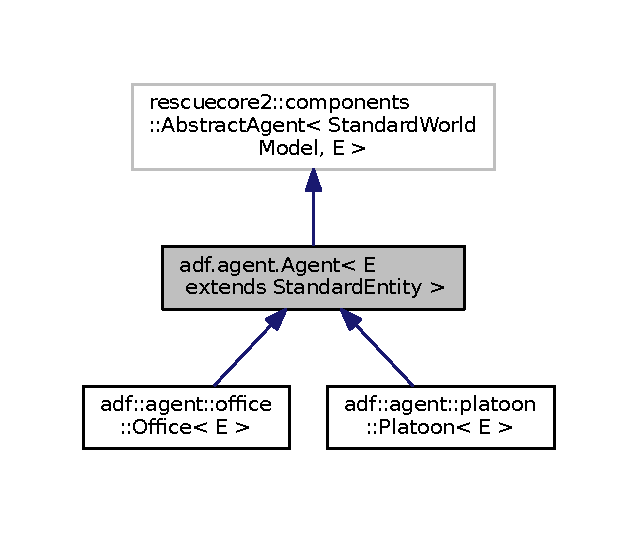
\includegraphics[width=306pt]{classadf_1_1agent_1_1Agent__inherit__graph}
\end{center}
\end{figure}


Collaboration diagram for adf.\+agent.\+Agent$<$ E extends Standard\+Entity $>$\+:
\nopagebreak
\begin{figure}[H]
\begin{center}
\leavevmode
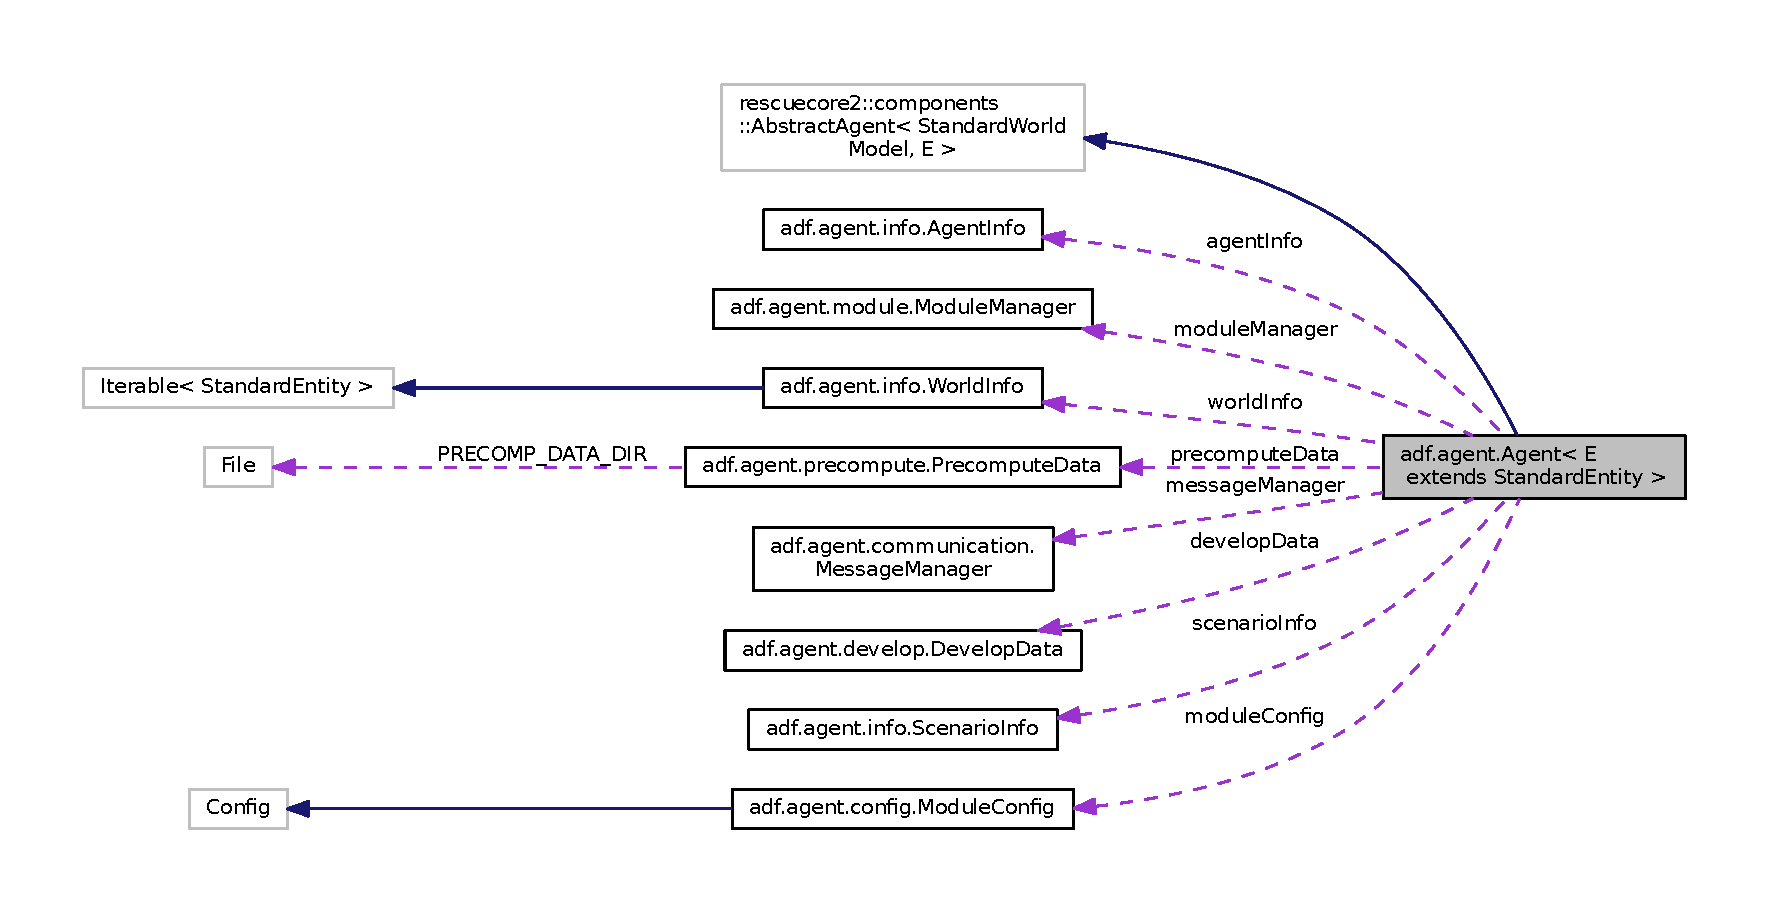
\includegraphics[width=350pt]{classadf_1_1agent_1_1Agent__coll__graph}
\end{center}
\end{figure}
\subsection*{Public Member Functions}
\begin{DoxyCompactItemize}
\item 
\hypertarget{classadf_1_1agent_1_1Agent_ababeb55c6e8dd72407db4f392b1d25e9}{}\label{classadf_1_1agent_1_1Agent_ababeb55c6e8dd72407db4f392b1d25e9} 
{\bfseries Agent} (String module\+Config\+File\+Name, boolean is\+Precompute, String data\+Storage\+Name, boolean is\+Debug\+Mode, \hyperlink{classadf_1_1agent_1_1develop_1_1DevelopData}{Develop\+Data} develop\+Data)
\item 
\hypertarget{classadf_1_1agent_1_1Agent_a39ccb85e5b206e0e521fb20d865cbefd}{}\label{classadf_1_1agent_1_1Agent_a39ccb85e5b206e0e521fb20d865cbefd} 
final String \mbox{[}$\,$\mbox{]} {\bfseries get\+Requested\+Entity\+U\+R\+Ns} ()
\item 
\hypertarget{classadf_1_1agent_1_1Agent_a09eb35626bb940da8a0b5d48ea098682}{}\label{classadf_1_1agent_1_1Agent_a09eb35626bb940da8a0b5d48ea098682} 
double {\bfseries getX} ()
\item 
\hypertarget{classadf_1_1agent_1_1Agent_a5161c268c9a7dd0382db84b7592c08f6}{}\label{classadf_1_1agent_1_1Agent_a5161c268c9a7dd0382db84b7592c08f6} 
double {\bfseries getY} ()
\item 
\hypertarget{classadf_1_1agent_1_1Agent_ac1c04c3453252af7754dff684091fdc3}{}\label{classadf_1_1agent_1_1Agent_ac1c04c3453252af7754dff684091fdc3} 
void {\bfseries send} (Message\mbox{[}$\,$\mbox{]} messages)
\item 
\hypertarget{classadf_1_1agent_1_1Agent_a4b7a389a5f8c0ae1dc60e7831de59833}{}\label{classadf_1_1agent_1_1Agent_a4b7a389a5f8c0ae1dc60e7831de59833} 
void {\bfseries send} (List$<$ Message $>$ messages)
\end{DoxyCompactItemize}
\subsection*{Public Attributes}
\begin{DoxyCompactItemize}
\item 
\hypertarget{classadf_1_1agent_1_1Agent_aa547b5cd18770b2e9bc7460eea8f03a3}{}\label{classadf_1_1agent_1_1Agent_aa547b5cd18770b2e9bc7460eea8f03a3} 
\hyperlink{classadf_1_1agent_1_1info_1_1AgentInfo}{Agent\+Info} {\bfseries agent\+Info}
\item 
\hypertarget{classadf_1_1agent_1_1Agent_a5c9c233f23eec057d6e6e415d3dc77f5}{}\label{classadf_1_1agent_1_1Agent_a5c9c233f23eec057d6e6e415d3dc77f5} 
\hyperlink{classadf_1_1agent_1_1info_1_1WorldInfo}{World\+Info} {\bfseries world\+Info}
\item 
\hypertarget{classadf_1_1agent_1_1Agent_ac2e2e8cad945673ee941e29251bddfcb}{}\label{classadf_1_1agent_1_1Agent_ac2e2e8cad945673ee941e29251bddfcb} 
\hyperlink{classadf_1_1agent_1_1info_1_1ScenarioInfo}{Scenario\+Info} {\bfseries scenario\+Info}
\end{DoxyCompactItemize}
\subsection*{Protected Member Functions}
\begin{DoxyCompactItemize}
\item 
\hypertarget{classadf_1_1agent_1_1Agent_a311ff9a9ad4a99ced51102f2083a7780}{}\label{classadf_1_1agent_1_1Agent_a311ff9a9ad4a99ced51102f2083a7780} 
abstract Enum\+Set$<$ Standard\+Entity\+U\+RN $>$ {\bfseries get\+Requested\+Entity\+U\+R\+Ns\+Enum} ()
\item 
\hypertarget{classadf_1_1agent_1_1Agent_aa6b4050401a515f48021b1813ea10688}{}\label{classadf_1_1agent_1_1Agent_aa6b4050401a515f48021b1813ea10688} 
Standard\+World\+Model {\bfseries create\+World\+Model} ()
\item 
\hypertarget{classadf_1_1agent_1_1Agent_ae831d47d081d9b343ec6c65e99de740f}{}\label{classadf_1_1agent_1_1Agent_ae831d47d081d9b343ec6c65e99de740f} 
void {\bfseries post\+Connect} ()
\item 
\hypertarget{classadf_1_1agent_1_1Agent_a69c3456b3351a085b5d959e6929cf2fe}{}\label{classadf_1_1agent_1_1Agent_a69c3456b3351a085b5d959e6929cf2fe} 
void {\bfseries process\+Sense} (K\+A\+Sense sense)
\item 
\hypertarget{classadf_1_1agent_1_1Agent_a747001153f5d19bc89d6aa5d343250a6}{}\label{classadf_1_1agent_1_1Agent_a747001153f5d19bc89d6aa5d343250a6} 
void {\bfseries think} (int time, Change\+Set changed, Collection$<$ Command $>$ heard)
\item 
\hypertarget{classadf_1_1agent_1_1Agent_aedd52af7190bca51de58f182aacc3cfe}{}\label{classadf_1_1agent_1_1Agent_aedd52af7190bca51de58f182aacc3cfe} 
abstract void {\bfseries think} ()
\item 
\hypertarget{classadf_1_1agent_1_1Agent_a20be2c96d7b14136d354a84f45067410}{}\label{classadf_1_1agent_1_1Agent_a20be2c96d7b14136d354a84f45067410} 
boolean {\bfseries should\+Index} ()
\end{DoxyCompactItemize}
\subsection*{Protected Attributes}
\begin{DoxyCompactItemize}
\item 
\hypertarget{classadf_1_1agent_1_1Agent_a742ce916588b3d9686a8f9af22941171}{}\label{classadf_1_1agent_1_1Agent_a742ce916588b3d9686a8f9af22941171} 
\hyperlink{classadf_1_1agent_1_1config_1_1ModuleConfig}{Module\+Config} {\bfseries module\+Config}
\item 
\hypertarget{classadf_1_1agent_1_1Agent_a9672da27f8a8ba4368f1aa0f1ae51dff}{}\label{classadf_1_1agent_1_1Agent_a9672da27f8a8ba4368f1aa0f1ae51dff} 
\hyperlink{classadf_1_1agent_1_1module_1_1ModuleManager}{Module\+Manager} {\bfseries module\+Manager}
\item 
\hypertarget{classadf_1_1agent_1_1Agent_a68ec8f2d6c7787c5f1a056f1d53e9a55}{}\label{classadf_1_1agent_1_1Agent_a68ec8f2d6c7787c5f1a056f1d53e9a55} 
\hyperlink{classadf_1_1agent_1_1precompute_1_1PrecomputeData}{Precompute\+Data} {\bfseries precompute\+Data}
\item 
\hypertarget{classadf_1_1agent_1_1Agent_a6245e35611c0f61f9041677ac82ba639}{}\label{classadf_1_1agent_1_1Agent_a6245e35611c0f61f9041677ac82ba639} 
\hyperlink{classadf_1_1agent_1_1develop_1_1DevelopData}{Develop\+Data} {\bfseries develop\+Data}
\item 
\hypertarget{classadf_1_1agent_1_1Agent_ad23f72ac5147a977e95aca61bb1179fe}{}\label{classadf_1_1agent_1_1Agent_ad23f72ac5147a977e95aca61bb1179fe} 
\hyperlink{classadf_1_1agent_1_1communication_1_1MessageManager}{Message\+Manager} {\bfseries message\+Manager}
\item 
\hypertarget{classadf_1_1agent_1_1Agent_abae1aa26b7cb5017b23335a6e07c619b}{}\label{classadf_1_1agent_1_1Agent_abae1aa26b7cb5017b23335a6e07c619b} 
boolean {\bfseries is\+Precompute}
\item 
\hypertarget{classadf_1_1agent_1_1Agent_a803016c7e44e4d46c39887ed9ca59b97}{}\label{classadf_1_1agent_1_1Agent_a803016c7e44e4d46c39887ed9ca59b97} 
boolean {\bfseries is\+Debug\+Mode}
\end{DoxyCompactItemize}
\subsection*{Static Protected Attributes}
\begin{DoxyCompactItemize}
\item 
\hypertarget{classadf_1_1agent_1_1Agent_acd99fefd69e32605d1fc2924c96eead0}{}\label{classadf_1_1agent_1_1Agent_acd99fefd69e32605d1fc2924c96eead0} 
final static String {\bfseries D\+A\+T\+A\+S\+T\+O\+R\+A\+G\+E\+\_\+\+F\+I\+L\+E\+\_\+\+N\+A\+M\+E\+\_\+\+A\+M\+B\+U\+L\+A\+N\+CE} = \char`\"{}ambulance.\+bin\char`\"{}
\item 
\hypertarget{classadf_1_1agent_1_1Agent_a00421901d5b40dd510ff645de4ed6279}{}\label{classadf_1_1agent_1_1Agent_a00421901d5b40dd510ff645de4ed6279} 
final static String {\bfseries D\+A\+T\+A\+S\+T\+O\+R\+A\+G\+E\+\_\+\+F\+I\+L\+E\+\_\+\+N\+A\+M\+E\+\_\+\+F\+I\+RE} = \char`\"{}fire.\+bin\char`\"{}
\item 
\hypertarget{classadf_1_1agent_1_1Agent_adc72b242cd1a60a0f8274cbcb03728a3}{}\label{classadf_1_1agent_1_1Agent_adc72b242cd1a60a0f8274cbcb03728a3} 
final static String {\bfseries D\+A\+T\+A\+S\+T\+O\+R\+A\+G\+E\+\_\+\+F\+I\+L\+E\+\_\+\+N\+A\+M\+E\+\_\+\+P\+O\+L\+I\+CE} = \char`\"{}police.\+bin\char`\"{}
\end{DoxyCompactItemize}


The documentation for this class was generated from the following file\+:\begin{DoxyCompactItemize}
\item 
src/main/java/adf/agent/Agent.\+java\end{DoxyCompactItemize}

\hypertarget{classadf_1_1agent_1_1info_1_1AgentInfo}{}\section{adf.\+agent.\+info.\+Agent\+Info クラス}
\label{classadf_1_1agent_1_1info_1_1AgentInfo}\index{adf.\+agent.\+info.\+Agent\+Info@{adf.\+agent.\+info.\+Agent\+Info}}
\subsection*{公開メンバ関数}
\begin{DoxyCompactItemize}
\item 
\hypertarget{classadf_1_1agent_1_1info_1_1AgentInfo_ac47ac11456ed03e8b98e1bfdb064dd18}{}\label{classadf_1_1agent_1_1info_1_1AgentInfo_ac47ac11456ed03e8b98e1bfdb064dd18} 
{\bfseries Agent\+Info} (\hyperlink{classadf_1_1agent_1_1Agent}{Agent} agent, Standard\+World\+Model world, Config config)
\item 
\hypertarget{classadf_1_1agent_1_1info_1_1AgentInfo_ad71982be9431abce3530ef4622852b34}{}\label{classadf_1_1agent_1_1info_1_1AgentInfo_ad71982be9431abce3530ef4622852b34} 
void {\bfseries set\+Time} (int time)
\item 
\hypertarget{classadf_1_1agent_1_1info_1_1AgentInfo_a2d1b58a841fd0092b5810b98a61bb9bb}{}\label{classadf_1_1agent_1_1info_1_1AgentInfo_a2d1b58a841fd0092b5810b98a61bb9bb} 
int {\bfseries get\+Time} ()
\item 
\hypertarget{classadf_1_1agent_1_1info_1_1AgentInfo_a23b8ecd1a583015ab5b6734ef513368f}{}\label{classadf_1_1agent_1_1info_1_1AgentInfo_a23b8ecd1a583015ab5b6734ef513368f} 
void {\bfseries set\+Heard} (Collection$<$ Command $>$ heard)
\item 
\hypertarget{classadf_1_1agent_1_1info_1_1AgentInfo_aa1a2550f424cc19a8b4d01531f2c797a}{}\label{classadf_1_1agent_1_1info_1_1AgentInfo_aa1a2550f424cc19a8b4d01531f2c797a} 
Collection$<$ Command $>$ {\bfseries get\+Heard} ()
\item 
\hypertarget{classadf_1_1agent_1_1info_1_1AgentInfo_a378db4a943ea7e16821b4950a59dfacf}{}\label{classadf_1_1agent_1_1info_1_1AgentInfo_a378db4a943ea7e16821b4950a59dfacf} 
Entity\+ID {\bfseries get\+ID} ()
\item 
\hypertarget{classadf_1_1agent_1_1info_1_1AgentInfo_a091c4fe745d95da7b3415c8f20626230}{}\label{classadf_1_1agent_1_1info_1_1AgentInfo_a091c4fe745d95da7b3415c8f20626230} 
Standard\+Entity {\bfseries me} ()
\item 
\hypertarget{classadf_1_1agent_1_1info_1_1AgentInfo_a4ed5eba8b822332d06d151dadd5ba953}{}\label{classadf_1_1agent_1_1info_1_1AgentInfo_a4ed5eba8b822332d06d151dadd5ba953} 
double {\bfseries getX} ()
\item 
\hypertarget{classadf_1_1agent_1_1info_1_1AgentInfo_a3c368a98edf3219b66b03fcce86b7eeb}{}\label{classadf_1_1agent_1_1info_1_1AgentInfo_a3c368a98edf3219b66b03fcce86b7eeb} 
double {\bfseries getY} ()
\item 
\hypertarget{classadf_1_1agent_1_1info_1_1AgentInfo_a749267c8b12d5e206345f7b754925c16}{}\label{classadf_1_1agent_1_1info_1_1AgentInfo_a749267c8b12d5e206345f7b754925c16} 
Entity\+ID {\bfseries get\+Position} ()
\item 
\hypertarget{classadf_1_1agent_1_1info_1_1AgentInfo_a8e1f8015e29c723f977cfa64eee9db6b}{}\label{classadf_1_1agent_1_1info_1_1AgentInfo_a8e1f8015e29c723f977cfa64eee9db6b} 
Area {\bfseries get\+Position\+Area} ()
\item 
\hypertarget{classadf_1_1agent_1_1info_1_1AgentInfo_a2df7c9be9a65d6796952b74860fe655e}{}\label{classadf_1_1agent_1_1info_1_1AgentInfo_a2df7c9be9a65d6796952b74860fe655e} 
void {\bfseries set\+Changed} (Change\+Set changed)
\item 
\hypertarget{classadf_1_1agent_1_1info_1_1AgentInfo_a8ced695c70693675d0d1b65fc2bb5798}{}\label{classadf_1_1agent_1_1info_1_1AgentInfo_a8ced695c70693675d0d1b65fc2bb5798} 
Change\+Set {\bfseries get\+Changed} ()
\item 
\hypertarget{classadf_1_1agent_1_1info_1_1AgentInfo_abe66f0a428ce365f3c38504e7ec89046}{}\label{classadf_1_1agent_1_1info_1_1AgentInfo_abe66f0a428ce365f3c38504e7ec89046} 
Human {\bfseries someone\+On\+Board} ()
\item 
\hypertarget{classadf_1_1agent_1_1info_1_1AgentInfo_a3413ebc871d37b53ba0de67581605058}{}\label{classadf_1_1agent_1_1info_1_1AgentInfo_a3413ebc871d37b53ba0de67581605058} 
boolean {\bfseries is\+Water\+Defined} ()
\item 
\hypertarget{classadf_1_1agent_1_1info_1_1AgentInfo_adb5d3d2ccf79c87a8f266425da451a71}{}\label{classadf_1_1agent_1_1info_1_1AgentInfo_adb5d3d2ccf79c87a8f266425da451a71} 
int {\bfseries get\+Water} ()
\item 
\hypertarget{classadf_1_1agent_1_1info_1_1AgentInfo_ab0623e4d050cd2581c694083aeac18a0}{}\label{classadf_1_1agent_1_1info_1_1AgentInfo_ab0623e4d050cd2581c694083aeac18a0} 
\hyperlink{classadf_1_1agent_1_1action_1_1Action}{Action} {\bfseries get\+Executed\+Action} (int time)
\item 
\hypertarget{classadf_1_1agent_1_1info_1_1AgentInfo_ae384e6762b685e108a11fa70cc652ff5}{}\label{classadf_1_1agent_1_1info_1_1AgentInfo_ae384e6762b685e108a11fa70cc652ff5} 
void {\bfseries set\+Executed\+Action} (int time, \hyperlink{classadf_1_1agent_1_1action_1_1Action}{Action} action)
\end{DoxyCompactItemize}


このクラス詳解は次のファイルから抽出されました\+:\begin{DoxyCompactItemize}
\item 
src/main/java/adf/agent/info/Agent\+Info.\+java\end{DoxyCompactItemize}

\hypertarget{classadf_1_1launcher_1_1AgentLauncher}{}\section{adf.\+launcher.\+Agent\+Launcher Class Reference}
\label{classadf_1_1launcher_1_1AgentLauncher}\index{adf.\+launcher.\+Agent\+Launcher@{adf.\+launcher.\+Agent\+Launcher}}
\subsection*{Public Member Functions}
\begin{DoxyCompactItemize}
\item 
\hypertarget{classadf_1_1launcher_1_1AgentLauncher_af70a64943f3e3dc9af62f53f8aa110b5}{}\label{classadf_1_1launcher_1_1AgentLauncher_af70a64943f3e3dc9af62f53f8aa110b5} 
{\bfseries Agent\+Launcher} (String... args)  throws Class\+Not\+Found\+Exception, Class\+Cast\+Exception, Instantiation\+Exception, Illegal\+Access\+Exception     
\item 
\hypertarget{classadf_1_1launcher_1_1AgentLauncher_a949d5a6d55b71cb5fb7e3508e888499a}{}\label{classadf_1_1launcher_1_1AgentLauncher_a949d5a6d55b71cb5fb7e3508e888499a} 
void {\bfseries start} ()
\end{DoxyCompactItemize}


The documentation for this class was generated from the following file\+:\begin{DoxyCompactItemize}
\item 
src/main/java/adf/launcher/Agent\+Launcher.\+java\end{DoxyCompactItemize}

\hypertarget{classadf_1_1component_1_1module_1_1complex_1_1center_1_1AmbulanceTargetAllocation}{}\section{adf.\+component.\+module.\+complex.\+center.\+Ambulance\+Target\+Allocation Class Reference}
\label{classadf_1_1component_1_1module_1_1complex_1_1center_1_1AmbulanceTargetAllocation}\index{adf.\+component.\+module.\+complex.\+center.\+Ambulance\+Target\+Allocation@{adf.\+component.\+module.\+complex.\+center.\+Ambulance\+Target\+Allocation}}


Inheritance diagram for adf.\+component.\+module.\+complex.\+center.\+Ambulance\+Target\+Allocation\+:
\nopagebreak
\begin{figure}[H]
\begin{center}
\leavevmode
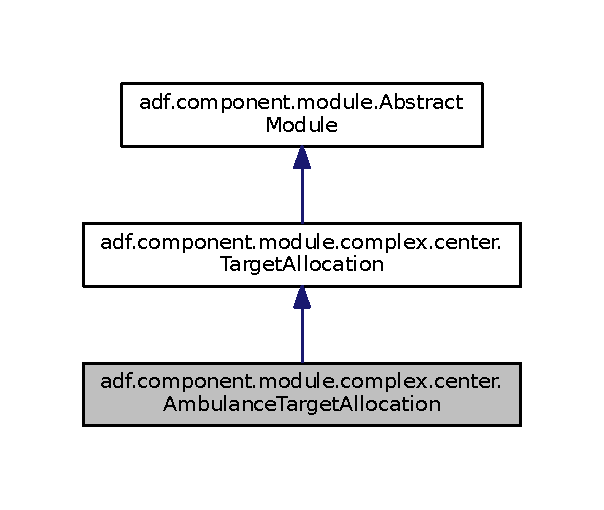
\includegraphics[width=290pt]{classadf_1_1component_1_1module_1_1complex_1_1center_1_1AmbulanceTargetAllocation__inherit__graph}
\end{center}
\end{figure}


Collaboration diagram for adf.\+component.\+module.\+complex.\+center.\+Ambulance\+Target\+Allocation\+:
\nopagebreak
\begin{figure}[H]
\begin{center}
\leavevmode
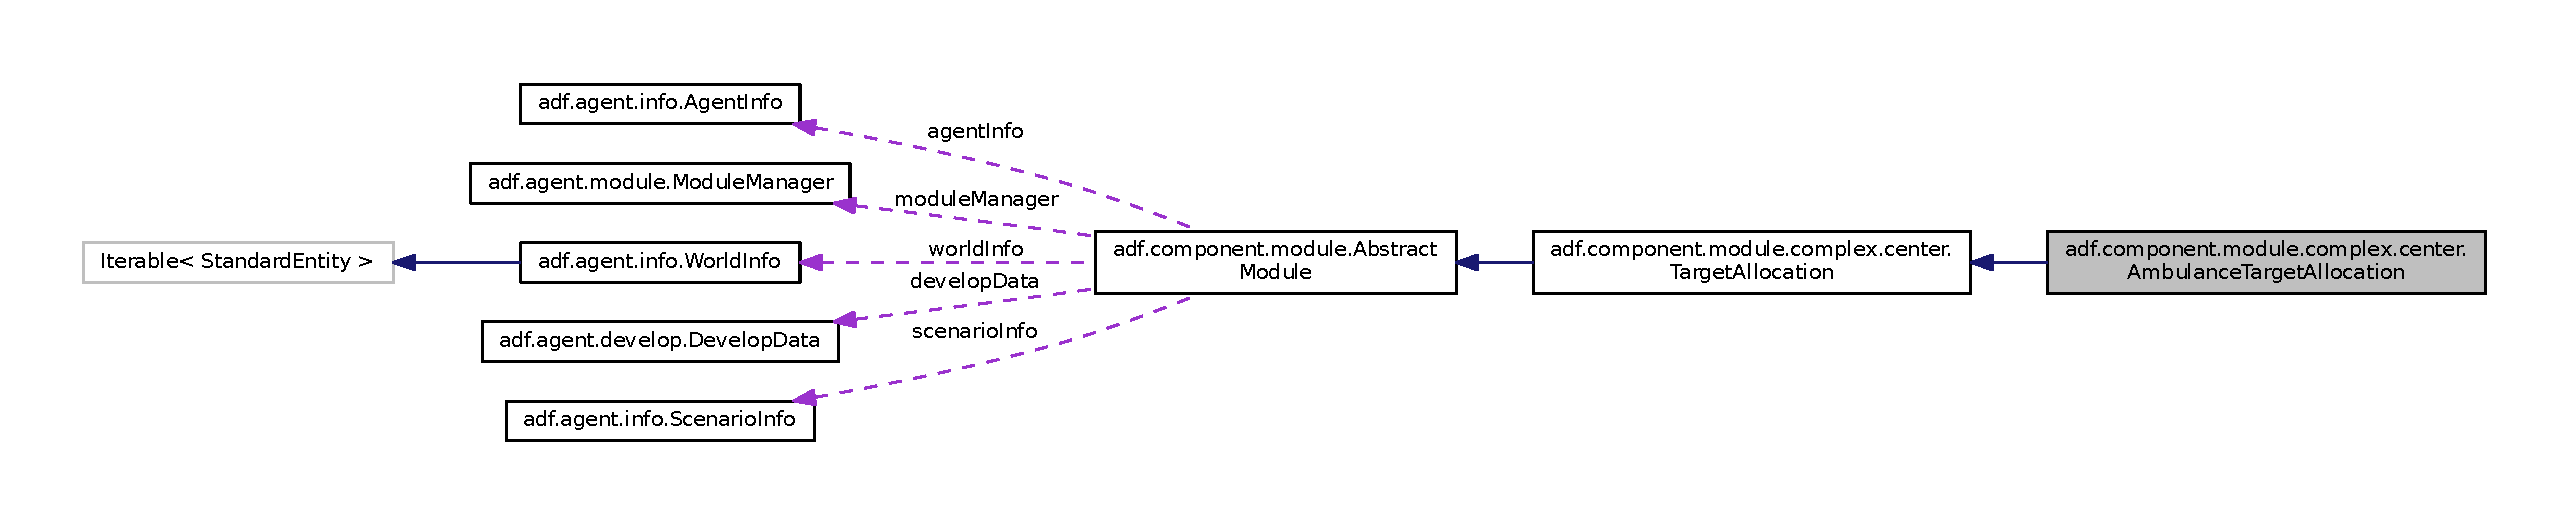
\includegraphics[width=350pt]{classadf_1_1component_1_1module_1_1complex_1_1center_1_1AmbulanceTargetAllocation__coll__graph}
\end{center}
\end{figure}
\subsection*{Public Member Functions}
\begin{DoxyCompactItemize}
\item 
\hypertarget{classadf_1_1component_1_1module_1_1complex_1_1center_1_1AmbulanceTargetAllocation_a060f3fdbcd0d0c67012875595b72bc36}{}\label{classadf_1_1component_1_1module_1_1complex_1_1center_1_1AmbulanceTargetAllocation_a060f3fdbcd0d0c67012875595b72bc36} 
{\bfseries Ambulance\+Target\+Allocation} (\hyperlink{classadf_1_1agent_1_1info_1_1AgentInfo}{Agent\+Info} ai, \hyperlink{classadf_1_1agent_1_1info_1_1WorldInfo}{World\+Info} wi, \hyperlink{classadf_1_1agent_1_1info_1_1ScenarioInfo}{Scenario\+Info} si, \hyperlink{classadf_1_1agent_1_1module_1_1ModuleManager}{Module\+Manager} module\+Manager, \hyperlink{classadf_1_1agent_1_1develop_1_1DevelopData}{Develop\+Data} develop\+Data)
\item 
\hypertarget{classadf_1_1component_1_1module_1_1complex_1_1center_1_1AmbulanceTargetAllocation_ad7cd1e24580e513d7536773e988661af}{}\label{classadf_1_1component_1_1module_1_1complex_1_1center_1_1AmbulanceTargetAllocation_ad7cd1e24580e513d7536773e988661af} 
abstract Map$<$ Entity\+ID, Entity\+ID $>$ {\bfseries get\+Result} ()
\item 
\hypertarget{classadf_1_1component_1_1module_1_1complex_1_1center_1_1AmbulanceTargetAllocation_a942779ce6569c48dfe20fb0fa8ab8e73}{}\label{classadf_1_1component_1_1module_1_1complex_1_1center_1_1AmbulanceTargetAllocation_a942779ce6569c48dfe20fb0fa8ab8e73} 
abstract \hyperlink{classadf_1_1component_1_1module_1_1complex_1_1center_1_1AmbulanceTargetAllocation}{Ambulance\+Target\+Allocation} {\bfseries calc} ()
\item 
\hypertarget{classadf_1_1component_1_1module_1_1complex_1_1center_1_1AmbulanceTargetAllocation_ab39c536442215cef75bd4187fde12f4b}{}\label{classadf_1_1component_1_1module_1_1complex_1_1center_1_1AmbulanceTargetAllocation_ab39c536442215cef75bd4187fde12f4b} 
\hyperlink{classadf_1_1component_1_1module_1_1complex_1_1center_1_1AmbulanceTargetAllocation}{Ambulance\+Target\+Allocation} {\bfseries precompute} (\hyperlink{classadf_1_1agent_1_1precompute_1_1PrecomputeData}{Precompute\+Data} precompute\+Data)
\item 
\hypertarget{classadf_1_1component_1_1module_1_1complex_1_1center_1_1AmbulanceTargetAllocation_a5fd9fa1a2c07fd5834bb9c26f868c57e}{}\label{classadf_1_1component_1_1module_1_1complex_1_1center_1_1AmbulanceTargetAllocation_a5fd9fa1a2c07fd5834bb9c26f868c57e} 
\hyperlink{classadf_1_1component_1_1module_1_1complex_1_1center_1_1AmbulanceTargetAllocation}{Ambulance\+Target\+Allocation} {\bfseries resume} (\hyperlink{classadf_1_1agent_1_1precompute_1_1PrecomputeData}{Precompute\+Data} precompute\+Data)
\item 
\hypertarget{classadf_1_1component_1_1module_1_1complex_1_1center_1_1AmbulanceTargetAllocation_ac26b7e2b96ea7e6840e0c91975547940}{}\label{classadf_1_1component_1_1module_1_1complex_1_1center_1_1AmbulanceTargetAllocation_ac26b7e2b96ea7e6840e0c91975547940} 
\hyperlink{classadf_1_1component_1_1module_1_1complex_1_1center_1_1AmbulanceTargetAllocation}{Ambulance\+Target\+Allocation} {\bfseries preparate} ()
\item 
\hypertarget{classadf_1_1component_1_1module_1_1complex_1_1center_1_1AmbulanceTargetAllocation_a7e2b401a11a1021871b97390f89ad61f}{}\label{classadf_1_1component_1_1module_1_1complex_1_1center_1_1AmbulanceTargetAllocation_a7e2b401a11a1021871b97390f89ad61f} 
\hyperlink{classadf_1_1component_1_1module_1_1complex_1_1center_1_1AmbulanceTargetAllocation}{Ambulance\+Target\+Allocation} {\bfseries update\+Info} (\hyperlink{classadf_1_1agent_1_1communication_1_1MessageManager}{Message\+Manager} message\+Manager)
\end{DoxyCompactItemize}
\subsection*{Additional Inherited Members}


The documentation for this class was generated from the following file\+:\begin{DoxyCompactItemize}
\item 
src/main/java/adf/component/module/complex/center/Ambulance\+Target\+Allocation.\+java\end{DoxyCompactItemize}

\hypertarget{classadf_1_1component_1_1communication_1_1util_1_1BitOutputStream}{}\section{adf.\+component.\+communication.\+util.\+Bit\+Output\+Stream Class Reference}
\label{classadf_1_1component_1_1communication_1_1util_1_1BitOutputStream}\index{adf.\+component.\+communication.\+util.\+Bit\+Output\+Stream@{adf.\+component.\+communication.\+util.\+Bit\+Output\+Stream}}


Inheritance diagram for adf.\+component.\+communication.\+util.\+Bit\+Output\+Stream\+:
\nopagebreak
\begin{figure}[H]
\begin{center}
\leavevmode
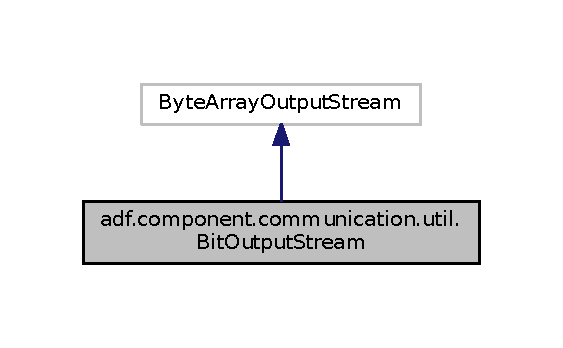
\includegraphics[width=270pt]{classadf_1_1component_1_1communication_1_1util_1_1BitOutputStream__inherit__graph}
\end{center}
\end{figure}


Collaboration diagram for adf.\+component.\+communication.\+util.\+Bit\+Output\+Stream\+:
\nopagebreak
\begin{figure}[H]
\begin{center}
\leavevmode
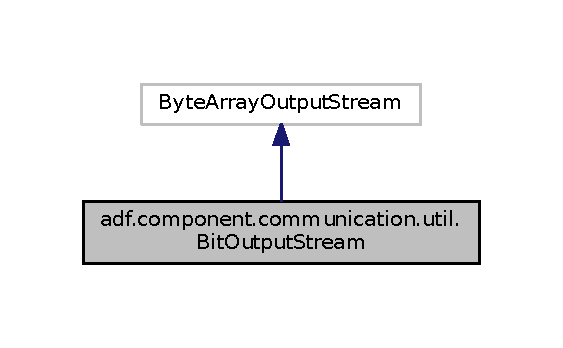
\includegraphics[width=270pt]{classadf_1_1component_1_1communication_1_1util_1_1BitOutputStream__coll__graph}
\end{center}
\end{figure}
\subsection*{Public Member Functions}
\begin{DoxyCompactItemize}
\item 
\hypertarget{classadf_1_1component_1_1communication_1_1util_1_1BitOutputStream_a931675a38ac9a042b61ad897c38ca2b1}{}\label{classadf_1_1component_1_1communication_1_1util_1_1BitOutputStream_a931675a38ac9a042b61ad897c38ca2b1} 
void {\bfseries reset} ()
\item 
\hypertarget{classadf_1_1component_1_1communication_1_1util_1_1BitOutputStream_acce75a559c869b003d1166858802d886}{}\label{classadf_1_1component_1_1communication_1_1util_1_1BitOutputStream_acce75a559c869b003d1166858802d886} 
synchronized void {\bfseries write} (int b)
\item 
\hypertarget{classadf_1_1component_1_1communication_1_1util_1_1BitOutputStream_aba842df4db5c7632cf4c884490aa451e}{}\label{classadf_1_1component_1_1communication_1_1util_1_1BitOutputStream_aba842df4db5c7632cf4c884490aa451e} 
synchronized void {\bfseries write\+Bits} (int value, int len)
\item 
\hypertarget{classadf_1_1component_1_1communication_1_1util_1_1BitOutputStream_a1b83277427bfd0477be1801d556a50ea}{}\label{classadf_1_1component_1_1communication_1_1util_1_1BitOutputStream_a1b83277427bfd0477be1801d556a50ea} 
synchronized void {\bfseries write\+Bits\+With\+Exist\+Flag} (int value, int len)
\item 
\hypertarget{classadf_1_1component_1_1communication_1_1util_1_1BitOutputStream_a8bc9b9b362cbd3526ddf04350d494ef4}{}\label{classadf_1_1component_1_1communication_1_1util_1_1BitOutputStream_a8bc9b9b362cbd3526ddf04350d494ef4} 
synchronized void {\bfseries write\+Null\+Flag} ()
\item 
\hypertarget{classadf_1_1component_1_1communication_1_1util_1_1BitOutputStream_a559168569088c244f06480df77c73b63}{}\label{classadf_1_1component_1_1communication_1_1util_1_1BitOutputStream_a559168569088c244f06480df77c73b63} 
synchronized int {\bfseries get\+Buffer} ()
\item 
\hypertarget{classadf_1_1component_1_1communication_1_1util_1_1BitOutputStream_a1940a7643ab8a3f85af54f29b2294421}{}\label{classadf_1_1component_1_1communication_1_1util_1_1BitOutputStream_a1940a7643ab8a3f85af54f29b2294421} 
synchronized void {\bfseries write\+Bits} (\hyperlink{classadf_1_1component_1_1communication_1_1util_1_1BitOutputStream}{Bit\+Output\+Stream} bos)
\item 
\hypertarget{classadf_1_1component_1_1communication_1_1util_1_1BitOutputStream_a6e40fa252db62c2c0e3cac9d0e1ca361}{}\label{classadf_1_1component_1_1communication_1_1util_1_1BitOutputStream_a6e40fa252db62c2c0e3cac9d0e1ca361} 
synchronized int {\bfseries size} ()
\item 
\hypertarget{classadf_1_1component_1_1communication_1_1util_1_1BitOutputStream_a87ce9be63be29582ee8f752ecc8e5e29}{}\label{classadf_1_1component_1_1communication_1_1util_1_1BitOutputStream_a87ce9be63be29582ee8f752ecc8e5e29} 
synchronized int {\bfseries get\+Bit\+Buffer\+Count} ()
\item 
\hypertarget{classadf_1_1component_1_1communication_1_1util_1_1BitOutputStream_ad39fb96d909ec14a93741479dd43934f}{}\label{classadf_1_1component_1_1communication_1_1util_1_1BitOutputStream_ad39fb96d909ec14a93741479dd43934f} 
synchronized byte \mbox{[}$\,$\mbox{]} {\bfseries to\+Byte\+Array} ()
\end{DoxyCompactItemize}


The documentation for this class was generated from the following file\+:\begin{DoxyCompactItemize}
\item 
src/main/java/adf/component/communication/util/Bit\+Output\+Stream.\+java\end{DoxyCompactItemize}

\hypertarget{classadf_1_1component_1_1communication_1_1util_1_1BitStreamReader}{}\section{adf.\+component.\+communication.\+util.\+Bit\+Stream\+Reader クラス}
\label{classadf_1_1component_1_1communication_1_1util_1_1BitStreamReader}\index{adf.\+component.\+communication.\+util.\+Bit\+Stream\+Reader@{adf.\+component.\+communication.\+util.\+Bit\+Stream\+Reader}}
\subsection*{公開メンバ関数}
\begin{DoxyCompactItemize}
\item 
\hypertarget{classadf_1_1component_1_1communication_1_1util_1_1BitStreamReader_aa675e7b62cbb86353d35e4501ce747a0}{}\label{classadf_1_1component_1_1communication_1_1util_1_1BitStreamReader_aa675e7b62cbb86353d35e4501ce747a0} 
{\bfseries Bit\+Stream\+Reader} (byte\mbox{[}$\,$\mbox{]} stream)
\item 
\hypertarget{classadf_1_1component_1_1communication_1_1util_1_1BitStreamReader_a35fa945440eb8d7020c719e1505b9e8d}{}\label{classadf_1_1component_1_1communication_1_1util_1_1BitStreamReader_a35fa945440eb8d7020c719e1505b9e8d} 
synchronized int {\bfseries get\+Bits} (int len)  throws Array\+Index\+Out\+Of\+Bounds\+Exception 
\item 
\hypertarget{classadf_1_1component_1_1communication_1_1util_1_1BitStreamReader_a86348d3f5ae3521b1b926d08b1ce4999}{}\label{classadf_1_1component_1_1communication_1_1util_1_1BitStreamReader_a86348d3f5ae3521b1b926d08b1ce4999} 
synchronized void {\bfseries write\+Back} (int len)
\item 
\hypertarget{classadf_1_1component_1_1communication_1_1util_1_1BitStreamReader_a9900873881f74452fd57a0ced23358de}{}\label{classadf_1_1component_1_1communication_1_1util_1_1BitStreamReader_a9900873881f74452fd57a0ced23358de} 
synchronized void {\bfseries write\+Forward} (int len)
\item 
\hypertarget{classadf_1_1component_1_1communication_1_1util_1_1BitStreamReader_ac2591f38dbbd31feeea3fbfcce95478b}{}\label{classadf_1_1component_1_1communication_1_1util_1_1BitStreamReader_ac2591f38dbbd31feeea3fbfcce95478b} 
final int {\bfseries index} ()
\item 
\hypertarget{classadf_1_1component_1_1communication_1_1util_1_1BitStreamReader_aac24549335f0248ac12dd8861e5dd426}{}\label{classadf_1_1component_1_1communication_1_1util_1_1BitStreamReader_aac24549335f0248ac12dd8861e5dd426} 
int {\bfseries get\+Remain\+Buffer} ()
\end{DoxyCompactItemize}


このクラス詳解は次のファイルから抽出されました\+:\begin{DoxyCompactItemize}
\item 
src/main/java/adf/component/communication/util/Bit\+Stream\+Reader.\+java\end{DoxyCompactItemize}

\hypertarget{classadf_1_1component_1_1module_1_1complex_1_1BuildingDetector}{}\section{adf.\+component.\+module.\+complex.\+Building\+Detector クラス}
\label{classadf_1_1component_1_1module_1_1complex_1_1BuildingDetector}\index{adf.\+component.\+module.\+complex.\+Building\+Detector@{adf.\+component.\+module.\+complex.\+Building\+Detector}}


adf.\+component.\+module.\+complex.\+Building\+Detector の継承関係図
\nopagebreak
\begin{figure}[H]
\begin{center}
\leavevmode
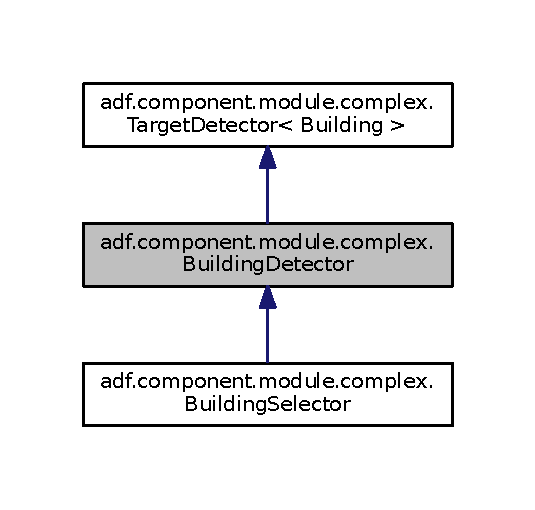
\includegraphics[width=257pt]{classadf_1_1component_1_1module_1_1complex_1_1BuildingDetector__inherit__graph}
\end{center}
\end{figure}


adf.\+component.\+module.\+complex.\+Building\+Detector 連携図
\nopagebreak
\begin{figure}[H]
\begin{center}
\leavevmode
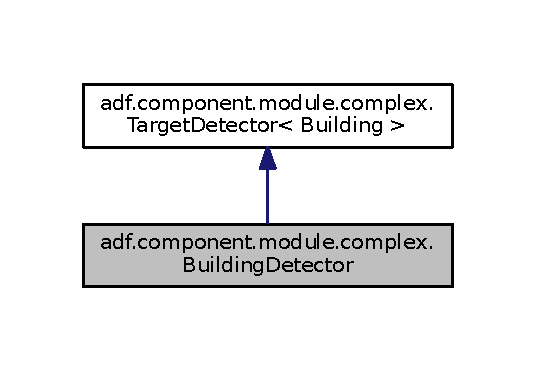
\includegraphics[width=257pt]{classadf_1_1component_1_1module_1_1complex_1_1BuildingDetector__coll__graph}
\end{center}
\end{figure}
\subsection*{公開メンバ関数}
\begin{DoxyCompactItemize}
\item 
\hypertarget{classadf_1_1component_1_1module_1_1complex_1_1BuildingDetector_aec293c18a386b5eb4b2790a172a4b658}{}\label{classadf_1_1component_1_1module_1_1complex_1_1BuildingDetector_aec293c18a386b5eb4b2790a172a4b658} 
{\bfseries Building\+Detector} (\hyperlink{classadf_1_1agent_1_1info_1_1AgentInfo}{Agent\+Info} ai, \hyperlink{classadf_1_1agent_1_1info_1_1WorldInfo}{World\+Info} wi, \hyperlink{classadf_1_1agent_1_1info_1_1ScenarioInfo}{Scenario\+Info} si, \hyperlink{classadf_1_1agent_1_1module_1_1ModuleManager}{Module\+Manager} module\+Manager, \hyperlink{classadf_1_1agent_1_1develop_1_1DevelopData}{Develop\+Data} develop\+Data)
\item 
\hypertarget{classadf_1_1component_1_1module_1_1complex_1_1BuildingDetector_ab2234c4c8272453eead244b01df179d3}{}\label{classadf_1_1component_1_1module_1_1complex_1_1BuildingDetector_ab2234c4c8272453eead244b01df179d3} 
\hyperlink{classadf_1_1component_1_1module_1_1complex_1_1BuildingDetector}{Building\+Detector} {\bfseries precompute} (\hyperlink{classadf_1_1agent_1_1precompute_1_1PrecomputeData}{Precompute\+Data} precompute\+Data)
\item 
\hypertarget{classadf_1_1component_1_1module_1_1complex_1_1BuildingDetector_a2f05d2f850a011165556239e27b0ac28}{}\label{classadf_1_1component_1_1module_1_1complex_1_1BuildingDetector_a2f05d2f850a011165556239e27b0ac28} 
\hyperlink{classadf_1_1component_1_1module_1_1complex_1_1BuildingDetector}{Building\+Detector} {\bfseries resume} (\hyperlink{classadf_1_1agent_1_1precompute_1_1PrecomputeData}{Precompute\+Data} precompute\+Data)
\item 
\hypertarget{classadf_1_1component_1_1module_1_1complex_1_1BuildingDetector_a335d77b425417f1c100f885e86df3854}{}\label{classadf_1_1component_1_1module_1_1complex_1_1BuildingDetector_a335d77b425417f1c100f885e86df3854} 
\hyperlink{classadf_1_1component_1_1module_1_1complex_1_1BuildingDetector}{Building\+Detector} {\bfseries preparate} ()
\item 
\hypertarget{classadf_1_1component_1_1module_1_1complex_1_1BuildingDetector_adc80809fbcc1981ee903ea82e282bf2b}{}\label{classadf_1_1component_1_1module_1_1complex_1_1BuildingDetector_adc80809fbcc1981ee903ea82e282bf2b} 
\hyperlink{classadf_1_1component_1_1module_1_1complex_1_1BuildingDetector}{Building\+Detector} {\bfseries update\+Info} (\hyperlink{classadf_1_1agent_1_1communication_1_1MessageManager}{Message\+Manager} message\+Manager)
\item 
\hypertarget{classadf_1_1component_1_1module_1_1complex_1_1BuildingDetector_a5bf336bb16e60b3c29b2d640366daf0d}{}\label{classadf_1_1component_1_1module_1_1complex_1_1BuildingDetector_a5bf336bb16e60b3c29b2d640366daf0d} 
abstract \hyperlink{classadf_1_1component_1_1module_1_1complex_1_1BuildingDetector}{Building\+Detector} {\bfseries calc} ()
\end{DoxyCompactItemize}


このクラス詳解は次のファイルから抽出されました\+:\begin{DoxyCompactItemize}
\item 
src/main/java/adf/component/module/complex/Building\+Detector.\+java\end{DoxyCompactItemize}

\hypertarget{classadf_1_1component_1_1module_1_1complex_1_1BuildingSelector}{}\section{adf.\+component.\+module.\+complex.\+Building\+Selector クラス}
\label{classadf_1_1component_1_1module_1_1complex_1_1BuildingSelector}\index{adf.\+component.\+module.\+complex.\+Building\+Selector@{adf.\+component.\+module.\+complex.\+Building\+Selector}}


adf.\+component.\+module.\+complex.\+Building\+Selector の継承関係図
\nopagebreak
\begin{figure}[H]
\begin{center}
\leavevmode
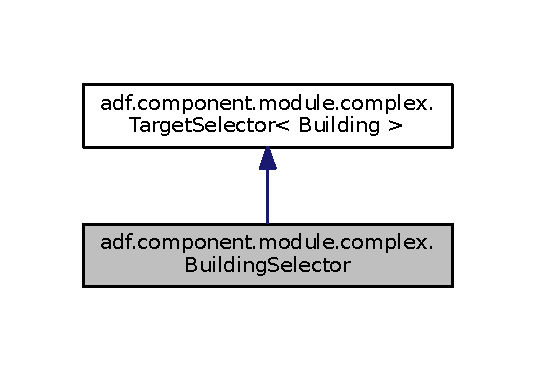
\includegraphics[width=257pt]{classadf_1_1component_1_1module_1_1complex_1_1BuildingSelector__inherit__graph}
\end{center}
\end{figure}


adf.\+component.\+module.\+complex.\+Building\+Selector 連携図
\nopagebreak
\begin{figure}[H]
\begin{center}
\leavevmode
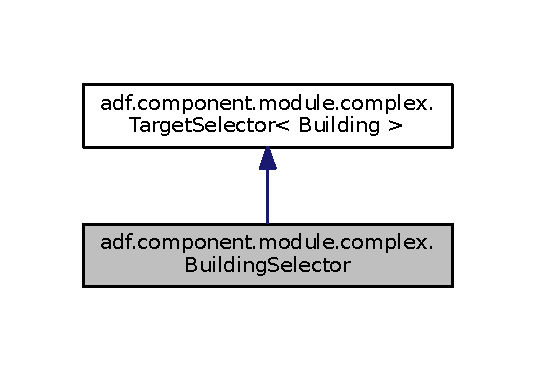
\includegraphics[width=257pt]{classadf_1_1component_1_1module_1_1complex_1_1BuildingSelector__coll__graph}
\end{center}
\end{figure}
\subsection*{公開メンバ関数}
\begin{DoxyCompactItemize}
\item 
\hypertarget{classadf_1_1component_1_1module_1_1complex_1_1BuildingSelector_accb98a3dc072b53332144c0570eea713}{}\label{classadf_1_1component_1_1module_1_1complex_1_1BuildingSelector_accb98a3dc072b53332144c0570eea713} 
{\bfseries Building\+Selector} (\hyperlink{classadf_1_1agent_1_1info_1_1AgentInfo}{Agent\+Info} ai, \hyperlink{classadf_1_1agent_1_1info_1_1WorldInfo}{World\+Info} wi, \hyperlink{classadf_1_1agent_1_1info_1_1ScenarioInfo}{Scenario\+Info} si, \hyperlink{classadf_1_1agent_1_1module_1_1ModuleManager}{Module\+Manager} module\+Manager, \hyperlink{classadf_1_1agent_1_1develop_1_1DevelopData}{Develop\+Data} develop\+Data)
\item 
\hypertarget{classadf_1_1component_1_1module_1_1complex_1_1BuildingSelector_afe2f19fe29b3a57e3df4a003923d9cdf}{}\label{classadf_1_1component_1_1module_1_1complex_1_1BuildingSelector_afe2f19fe29b3a57e3df4a003923d9cdf} 
\hyperlink{classadf_1_1component_1_1module_1_1complex_1_1BuildingSelector}{Building\+Selector} {\bfseries precompute} (\hyperlink{classadf_1_1agent_1_1precompute_1_1PrecomputeData}{Precompute\+Data} precompute\+Data)
\item 
\hypertarget{classadf_1_1component_1_1module_1_1complex_1_1BuildingSelector_ab23c92d96da847e1a9218a7fb50e6098}{}\label{classadf_1_1component_1_1module_1_1complex_1_1BuildingSelector_ab23c92d96da847e1a9218a7fb50e6098} 
\hyperlink{classadf_1_1component_1_1module_1_1complex_1_1BuildingSelector}{Building\+Selector} {\bfseries resume} (\hyperlink{classadf_1_1agent_1_1precompute_1_1PrecomputeData}{Precompute\+Data} precompute\+Data)
\item 
\hypertarget{classadf_1_1component_1_1module_1_1complex_1_1BuildingSelector_a01457e08066eb8bf50fe521df437c03e}{}\label{classadf_1_1component_1_1module_1_1complex_1_1BuildingSelector_a01457e08066eb8bf50fe521df437c03e} 
\hyperlink{classadf_1_1component_1_1module_1_1complex_1_1BuildingSelector}{Building\+Selector} {\bfseries preparate} ()
\item 
\hypertarget{classadf_1_1component_1_1module_1_1complex_1_1BuildingSelector_af80b6a108c9d3741c2e8d11b4fb3cf98}{}\label{classadf_1_1component_1_1module_1_1complex_1_1BuildingSelector_af80b6a108c9d3741c2e8d11b4fb3cf98} 
\hyperlink{classadf_1_1component_1_1module_1_1complex_1_1BuildingSelector}{Building\+Selector} {\bfseries update\+Info} (\hyperlink{classadf_1_1agent_1_1communication_1_1MessageManager}{Message\+Manager} message\+Manager)
\item 
\hypertarget{classadf_1_1component_1_1module_1_1complex_1_1BuildingSelector_a4366ea9047a409d4b96d78aa976b6781}{}\label{classadf_1_1component_1_1module_1_1complex_1_1BuildingSelector_a4366ea9047a409d4b96d78aa976b6781} 
abstract \hyperlink{classadf_1_1component_1_1module_1_1complex_1_1BuildingSelector}{Building\+Selector} {\bfseries calc} ()
\end{DoxyCompactItemize}


このクラス詳解は次のファイルから抽出されました\+:\begin{DoxyCompactItemize}
\item 
src/main/java/adf/component/module/complex/Building\+Selector.\+java\end{DoxyCompactItemize}

\hypertarget{classadf_1_1component_1_1module_1_1algorithm_1_1Clustering}{}\section{adf.\+component.\+module.\+algorithm.\+Clustering クラス}
\label{classadf_1_1component_1_1module_1_1algorithm_1_1Clustering}\index{adf.\+component.\+module.\+algorithm.\+Clustering@{adf.\+component.\+module.\+algorithm.\+Clustering}}


adf.\+component.\+module.\+algorithm.\+Clustering の継承関係図
\nopagebreak
\begin{figure}[H]
\begin{center}
\leavevmode
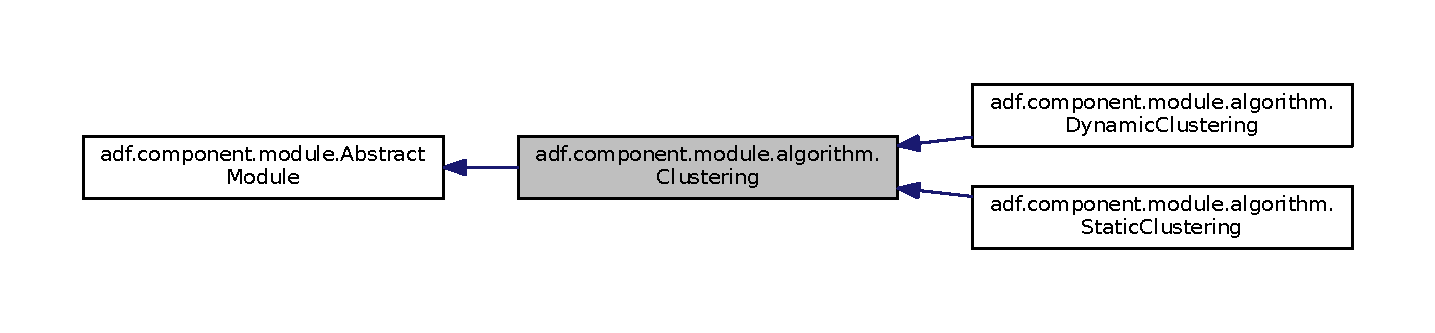
\includegraphics[width=350pt]{classadf_1_1component_1_1module_1_1algorithm_1_1Clustering__inherit__graph}
\end{center}
\end{figure}


adf.\+component.\+module.\+algorithm.\+Clustering 連携図
\nopagebreak
\begin{figure}[H]
\begin{center}
\leavevmode
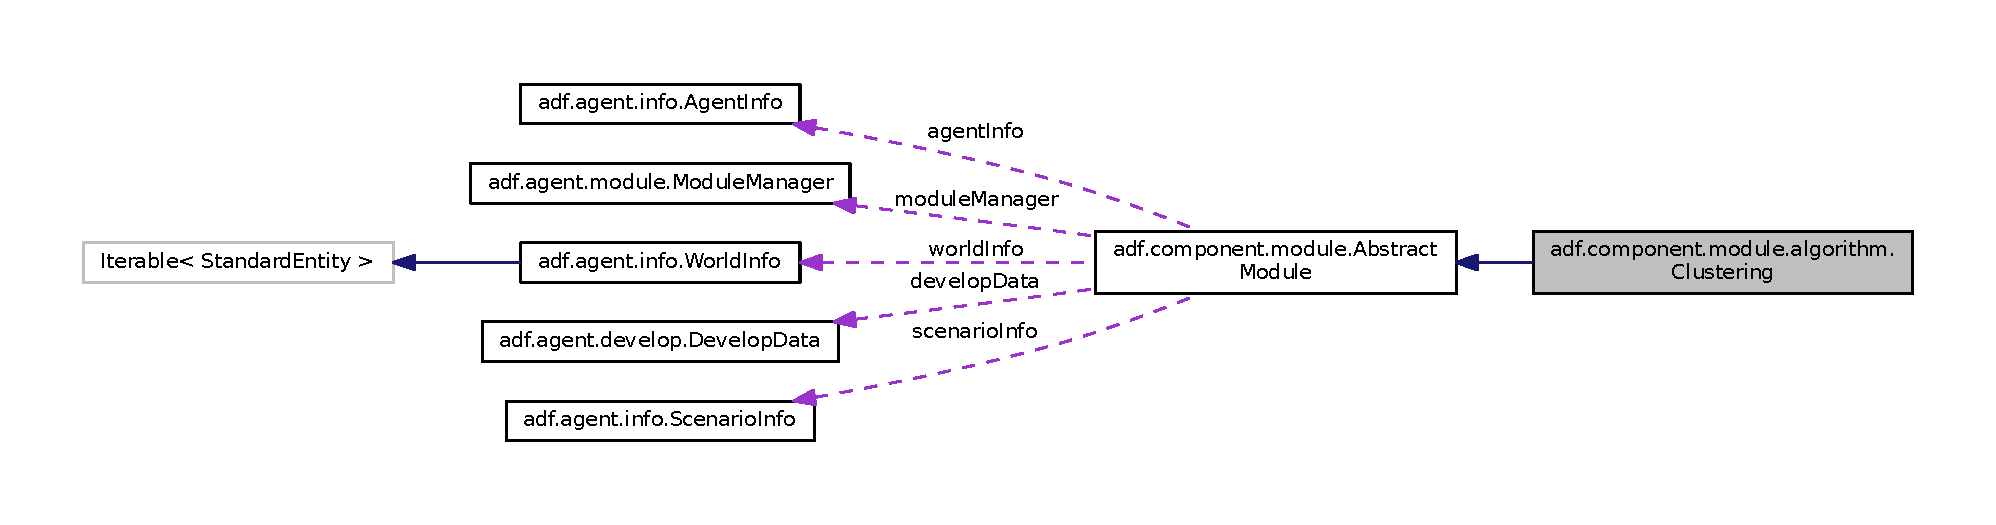
\includegraphics[width=350pt]{classadf_1_1component_1_1module_1_1algorithm_1_1Clustering__coll__graph}
\end{center}
\end{figure}
\subsection*{公開メンバ関数}
\begin{DoxyCompactItemize}
\item 
\hypertarget{classadf_1_1component_1_1module_1_1algorithm_1_1Clustering_aa1dcf3e542dafd76e7a60937d5ef1a65}{}\label{classadf_1_1component_1_1module_1_1algorithm_1_1Clustering_aa1dcf3e542dafd76e7a60937d5ef1a65} 
{\bfseries Clustering} (\hyperlink{classadf_1_1agent_1_1info_1_1AgentInfo}{Agent\+Info} ai, \hyperlink{classadf_1_1agent_1_1info_1_1WorldInfo}{World\+Info} wi, \hyperlink{classadf_1_1agent_1_1info_1_1ScenarioInfo}{Scenario\+Info} si, \hyperlink{classadf_1_1agent_1_1module_1_1ModuleManager}{Module\+Manager} module\+Manager, \hyperlink{classadf_1_1agent_1_1develop_1_1DevelopData}{Develop\+Data} develop\+Data)
\item 
\hypertarget{classadf_1_1component_1_1module_1_1algorithm_1_1Clustering_a11645f349c9d8b3b36a5bd0ef32c8759}{}\label{classadf_1_1component_1_1module_1_1algorithm_1_1Clustering_a11645f349c9d8b3b36a5bd0ef32c8759} 
abstract int {\bfseries get\+Cluster\+Number} ()
\item 
\hypertarget{classadf_1_1component_1_1module_1_1algorithm_1_1Clustering_a95e78c67ee2faf449f268d3de54356ed}{}\label{classadf_1_1component_1_1module_1_1algorithm_1_1Clustering_a95e78c67ee2faf449f268d3de54356ed} 
abstract int {\bfseries get\+Cluster\+Index} (Standard\+Entity entity)
\item 
\hypertarget{classadf_1_1component_1_1module_1_1algorithm_1_1Clustering_adf11ac7549acf8c5f6f5b8ce940b7a29}{}\label{classadf_1_1component_1_1module_1_1algorithm_1_1Clustering_adf11ac7549acf8c5f6f5b8ce940b7a29} 
abstract int {\bfseries get\+Cluster\+Index} (Entity\+ID id)
\item 
\hypertarget{classadf_1_1component_1_1module_1_1algorithm_1_1Clustering_a48736807ea1eb28cea5537b9cd92c432}{}\label{classadf_1_1component_1_1module_1_1algorithm_1_1Clustering_a48736807ea1eb28cea5537b9cd92c432} 
abstract Collection$<$ Standard\+Entity $>$ {\bfseries get\+Cluster\+Entities} (int index)
\item 
\hypertarget{classadf_1_1component_1_1module_1_1algorithm_1_1Clustering_a8b93e3382f702875cb9d0380bc5fa082}{}\label{classadf_1_1component_1_1module_1_1algorithm_1_1Clustering_a8b93e3382f702875cb9d0380bc5fa082} 
abstract Collection$<$ Entity\+ID $>$ {\bfseries get\+Cluster\+Entity\+I\+Ds} (int index)
\item 
\hypertarget{classadf_1_1component_1_1module_1_1algorithm_1_1Clustering_aa7924939f7d3f73322619ba5d60f2ea1}{}\label{classadf_1_1component_1_1module_1_1algorithm_1_1Clustering_aa7924939f7d3f73322619ba5d60f2ea1} 
\hyperlink{classadf_1_1component_1_1module_1_1algorithm_1_1Clustering}{Clustering} {\bfseries precompute} (\hyperlink{classadf_1_1agent_1_1precompute_1_1PrecomputeData}{Precompute\+Data} precompute\+Data)
\item 
\hypertarget{classadf_1_1component_1_1module_1_1algorithm_1_1Clustering_ab3e78f078f6b73a8581dab6fb64a13ad}{}\label{classadf_1_1component_1_1module_1_1algorithm_1_1Clustering_ab3e78f078f6b73a8581dab6fb64a13ad} 
\hyperlink{classadf_1_1component_1_1module_1_1algorithm_1_1Clustering}{Clustering} {\bfseries resume} (\hyperlink{classadf_1_1agent_1_1precompute_1_1PrecomputeData}{Precompute\+Data} precompute\+Data)
\item 
\hypertarget{classadf_1_1component_1_1module_1_1algorithm_1_1Clustering_a7d4daee07eecc0fb80f9dcc070dbfd42}{}\label{classadf_1_1component_1_1module_1_1algorithm_1_1Clustering_a7d4daee07eecc0fb80f9dcc070dbfd42} 
\hyperlink{classadf_1_1component_1_1module_1_1algorithm_1_1Clustering}{Clustering} {\bfseries preparate} ()
\item 
\hypertarget{classadf_1_1component_1_1module_1_1algorithm_1_1Clustering_a9518f4cfcc587897cf05170f399d1a7c}{}\label{classadf_1_1component_1_1module_1_1algorithm_1_1Clustering_a9518f4cfcc587897cf05170f399d1a7c} 
\hyperlink{classadf_1_1component_1_1module_1_1algorithm_1_1Clustering}{Clustering} {\bfseries update\+Info} (\hyperlink{classadf_1_1agent_1_1communication_1_1MessageManager}{Message\+Manager} message\+Manager)
\item 
\hypertarget{classadf_1_1component_1_1module_1_1algorithm_1_1Clustering_ab0323479531d10738a0cf25a3b5d3117}{}\label{classadf_1_1component_1_1module_1_1algorithm_1_1Clustering_ab0323479531d10738a0cf25a3b5d3117} 
abstract \hyperlink{classadf_1_1component_1_1module_1_1algorithm_1_1Clustering}{Clustering} {\bfseries calc} ()
\end{DoxyCompactItemize}
\subsection*{その他の継承メンバ}


このクラス詳解は次のファイルから抽出されました\+:\begin{DoxyCompactItemize}
\item 
src/main/java/adf/component/module/algorithm/Clustering.\+java\end{DoxyCompactItemize}

\hypertarget{classadf_1_1agent_1_1communication_1_1standard_1_1bundle_1_1centralized_1_1CommandAmbulance}{}\section{adf.\+agent.\+communication.\+standard.\+bundle.\+centralized.\+Command\+Ambulance Class Reference}
\label{classadf_1_1agent_1_1communication_1_1standard_1_1bundle_1_1centralized_1_1CommandAmbulance}\index{adf.\+agent.\+communication.\+standard.\+bundle.\+centralized.\+Command\+Ambulance@{adf.\+agent.\+communication.\+standard.\+bundle.\+centralized.\+Command\+Ambulance}}


Inheritance diagram for adf.\+agent.\+communication.\+standard.\+bundle.\+centralized.\+Command\+Ambulance\+:
\nopagebreak
\begin{figure}[H]
\begin{center}
\leavevmode
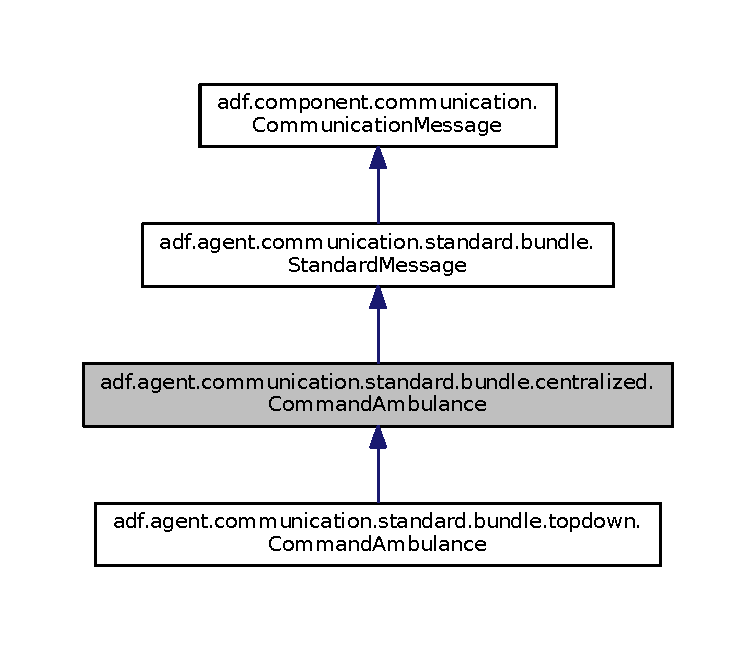
\includegraphics[width=350pt]{classadf_1_1agent_1_1communication_1_1standard_1_1bundle_1_1centralized_1_1CommandAmbulance__inherit__graph}
\end{center}
\end{figure}


Collaboration diagram for adf.\+agent.\+communication.\+standard.\+bundle.\+centralized.\+Command\+Ambulance\+:
\nopagebreak
\begin{figure}[H]
\begin{center}
\leavevmode
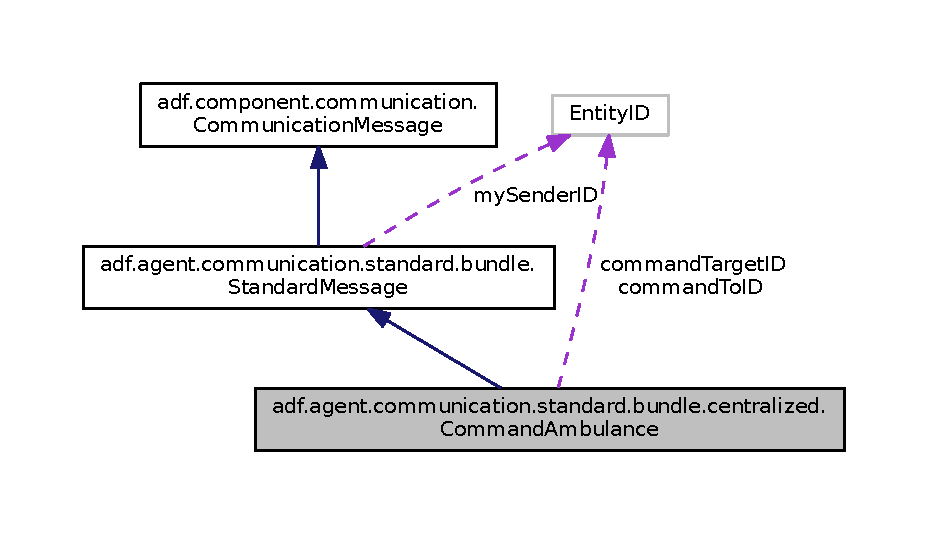
\includegraphics[width=350pt]{classadf_1_1agent_1_1communication_1_1standard_1_1bundle_1_1centralized_1_1CommandAmbulance__coll__graph}
\end{center}
\end{figure}
\subsection*{Public Member Functions}
\begin{DoxyCompactItemize}
\item 
\hypertarget{classadf_1_1agent_1_1communication_1_1standard_1_1bundle_1_1centralized_1_1CommandAmbulance_af4c58ca174dd264b77e8437cd349f7d5}{}\label{classadf_1_1agent_1_1communication_1_1standard_1_1bundle_1_1centralized_1_1CommandAmbulance_af4c58ca174dd264b77e8437cd349f7d5} 
{\bfseries Command\+Ambulance} (boolean is\+Radio, Entity\+ID to\+ID, Entity\+ID target\+ID, int action)
\item 
\hypertarget{classadf_1_1agent_1_1communication_1_1standard_1_1bundle_1_1centralized_1_1CommandAmbulance_a48208b238525c43b3b343f574b14608d}{}\label{classadf_1_1agent_1_1communication_1_1standard_1_1bundle_1_1centralized_1_1CommandAmbulance_a48208b238525c43b3b343f574b14608d} 
{\bfseries Command\+Ambulance} (boolean is\+Radio, int from, int ttl, \hyperlink{classadf_1_1component_1_1communication_1_1util_1_1BitStreamReader}{Bit\+Stream\+Reader} bit\+Stream\+Reader)
\item 
\hypertarget{classadf_1_1agent_1_1communication_1_1standard_1_1bundle_1_1centralized_1_1CommandAmbulance_a0fdaa5d090d6c487e2c7664e190160e1}{}\label{classadf_1_1agent_1_1communication_1_1standard_1_1bundle_1_1centralized_1_1CommandAmbulance_a0fdaa5d090d6c487e2c7664e190160e1} 
int {\bfseries get\+Action} ()
\item 
\hypertarget{classadf_1_1agent_1_1communication_1_1standard_1_1bundle_1_1centralized_1_1CommandAmbulance_aaf0888999907ffc19c94654fb56cbefb}{}\label{classadf_1_1agent_1_1communication_1_1standard_1_1bundle_1_1centralized_1_1CommandAmbulance_aaf0888999907ffc19c94654fb56cbefb} 
int {\bfseries get\+Byte\+Array\+Size} ()
\item 
\hypertarget{classadf_1_1agent_1_1communication_1_1standard_1_1bundle_1_1centralized_1_1CommandAmbulance_ae22089145f07edd60988c11068d511eb}{}\label{classadf_1_1agent_1_1communication_1_1standard_1_1bundle_1_1centralized_1_1CommandAmbulance_ae22089145f07edd60988c11068d511eb} 
byte \mbox{[}$\,$\mbox{]} {\bfseries to\+Byte\+Array} ()
\item 
\hypertarget{classadf_1_1agent_1_1communication_1_1standard_1_1bundle_1_1centralized_1_1CommandAmbulance_a8bc9847a401dbf94039f2ca30cc36590}{}\label{classadf_1_1agent_1_1communication_1_1standard_1_1bundle_1_1centralized_1_1CommandAmbulance_a8bc9847a401dbf94039f2ca30cc36590} 
\hyperlink{classadf_1_1component_1_1communication_1_1util_1_1BitOutputStream}{Bit\+Output\+Stream} {\bfseries to\+Bit\+Output\+Stream} ()
\item 
\hypertarget{classadf_1_1agent_1_1communication_1_1standard_1_1bundle_1_1centralized_1_1CommandAmbulance_a0d24a2d60d460a2dd8e708912ff8c754}{}\label{classadf_1_1agent_1_1communication_1_1standard_1_1bundle_1_1centralized_1_1CommandAmbulance_a0d24a2d60d460a2dd8e708912ff8c754} 
Entity\+ID {\bfseries get\+To\+ID} ()
\item 
\hypertarget{classadf_1_1agent_1_1communication_1_1standard_1_1bundle_1_1centralized_1_1CommandAmbulance_a4b334a04059f03321eec9b279c0f6018}{}\label{classadf_1_1agent_1_1communication_1_1standard_1_1bundle_1_1centralized_1_1CommandAmbulance_a4b334a04059f03321eec9b279c0f6018} 
Entity\+ID {\bfseries get\+Target\+ID} ()
\item 
\hypertarget{classadf_1_1agent_1_1communication_1_1standard_1_1bundle_1_1centralized_1_1CommandAmbulance_a518fa51ce2cfa7847ce1f570e91d0044}{}\label{classadf_1_1agent_1_1communication_1_1standard_1_1bundle_1_1centralized_1_1CommandAmbulance_a518fa51ce2cfa7847ce1f570e91d0044} 
boolean {\bfseries is\+Broadcast} ()
\item 
\hypertarget{classadf_1_1agent_1_1communication_1_1standard_1_1bundle_1_1centralized_1_1CommandAmbulance_ae755d171b6e2142716e23a10a1afc7a3}{}\label{classadf_1_1agent_1_1communication_1_1standard_1_1bundle_1_1centralized_1_1CommandAmbulance_ae755d171b6e2142716e23a10a1afc7a3} 
boolean {\bfseries is\+To\+I\+D\+Defined} ()
\item 
\hypertarget{classadf_1_1agent_1_1communication_1_1standard_1_1bundle_1_1centralized_1_1CommandAmbulance_a2c573fa72579ddbcb559f1ea2421a4ee}{}\label{classadf_1_1agent_1_1communication_1_1standard_1_1bundle_1_1centralized_1_1CommandAmbulance_a2c573fa72579ddbcb559f1ea2421a4ee} 
boolean {\bfseries id\+Target\+I\+D\+Defined} ()
\item 
\hypertarget{classadf_1_1agent_1_1communication_1_1standard_1_1bundle_1_1centralized_1_1CommandAmbulance_a4fe21b196047222b86926de53da07e63}{}\label{classadf_1_1agent_1_1communication_1_1standard_1_1bundle_1_1centralized_1_1CommandAmbulance_a4fe21b196047222b86926de53da07e63} 
String {\bfseries get\+Check\+Key} ()
\end{DoxyCompactItemize}
\subsection*{Static Public Attributes}
\begin{DoxyCompactItemize}
\item 
\hypertarget{classadf_1_1agent_1_1communication_1_1standard_1_1bundle_1_1centralized_1_1CommandAmbulance_a4466876a657551b0bdac92658301eee8}{}\label{classadf_1_1agent_1_1communication_1_1standard_1_1bundle_1_1centralized_1_1CommandAmbulance_a4466876a657551b0bdac92658301eee8} 
static final int {\bfseries A\+C\+T\+I\+O\+N\+\_\+\+R\+E\+ST} = 0
\item 
\hypertarget{classadf_1_1agent_1_1communication_1_1standard_1_1bundle_1_1centralized_1_1CommandAmbulance_a66aaf95b0ead18ae28f214fc1c6e5e7b}{}\label{classadf_1_1agent_1_1communication_1_1standard_1_1bundle_1_1centralized_1_1CommandAmbulance_a66aaf95b0ead18ae28f214fc1c6e5e7b} 
static final int {\bfseries A\+C\+T\+I\+O\+N\+\_\+\+M\+O\+VE} = 1
\item 
\hypertarget{classadf_1_1agent_1_1communication_1_1standard_1_1bundle_1_1centralized_1_1CommandAmbulance_acde97d04f8c30ea87a8d1ecac2f61b6e}{}\label{classadf_1_1agent_1_1communication_1_1standard_1_1bundle_1_1centralized_1_1CommandAmbulance_acde97d04f8c30ea87a8d1ecac2f61b6e} 
static final int {\bfseries A\+C\+T\+I\+O\+N\+\_\+\+R\+E\+S\+C\+UE} = 2
\item 
\hypertarget{classadf_1_1agent_1_1communication_1_1standard_1_1bundle_1_1centralized_1_1CommandAmbulance_a7bb0569ec2b1a9bdc4e337b862e1b042}{}\label{classadf_1_1agent_1_1communication_1_1standard_1_1bundle_1_1centralized_1_1CommandAmbulance_a7bb0569ec2b1a9bdc4e337b862e1b042} 
static final int {\bfseries A\+C\+T\+I\+O\+N\+\_\+\+L\+O\+AD} = 3
\item 
\hypertarget{classadf_1_1agent_1_1communication_1_1standard_1_1bundle_1_1centralized_1_1CommandAmbulance_a9ab11b46e57624515e8c314db4743370}{}\label{classadf_1_1agent_1_1communication_1_1standard_1_1bundle_1_1centralized_1_1CommandAmbulance_a9ab11b46e57624515e8c314db4743370} 
static final int {\bfseries A\+C\+T\+I\+O\+N\+\_\+\+U\+N\+L\+O\+AD} = 4
\item 
\hypertarget{classadf_1_1agent_1_1communication_1_1standard_1_1bundle_1_1centralized_1_1CommandAmbulance_a292b4f1302f9d061d4d1ecbd0cea7c59}{}\label{classadf_1_1agent_1_1communication_1_1standard_1_1bundle_1_1centralized_1_1CommandAmbulance_a292b4f1302f9d061d4d1ecbd0cea7c59} 
static final int {\bfseries A\+C\+T\+I\+O\+N\+\_\+\+A\+U\+T\+O\+N\+O\+MY} = 5
\end{DoxyCompactItemize}
\subsection*{Protected Attributes}
\begin{DoxyCompactItemize}
\item 
\hypertarget{classadf_1_1agent_1_1communication_1_1standard_1_1bundle_1_1centralized_1_1CommandAmbulance_a97e8b4990f2dc4993cf7a5d688ba75d0}{}\label{classadf_1_1agent_1_1communication_1_1standard_1_1bundle_1_1centralized_1_1CommandAmbulance_a97e8b4990f2dc4993cf7a5d688ba75d0} 
int {\bfseries raw\+To\+ID}
\item 
\hypertarget{classadf_1_1agent_1_1communication_1_1standard_1_1bundle_1_1centralized_1_1CommandAmbulance_aa4f86ac3f5617b3f738a04f0a53f12ea}{}\label{classadf_1_1agent_1_1communication_1_1standard_1_1bundle_1_1centralized_1_1CommandAmbulance_aa4f86ac3f5617b3f738a04f0a53f12ea} 
int {\bfseries raw\+Target\+ID}
\item 
\hypertarget{classadf_1_1agent_1_1communication_1_1standard_1_1bundle_1_1centralized_1_1CommandAmbulance_aaf63382e49a330ea42fd060dfdff00a2}{}\label{classadf_1_1agent_1_1communication_1_1standard_1_1bundle_1_1centralized_1_1CommandAmbulance_aaf63382e49a330ea42fd060dfdff00a2} 
Entity\+ID {\bfseries command\+To\+ID}
\item 
\hypertarget{classadf_1_1agent_1_1communication_1_1standard_1_1bundle_1_1centralized_1_1CommandAmbulance_a98e8a6ff76f44059b4ac618081b27dbe}{}\label{classadf_1_1agent_1_1communication_1_1standard_1_1bundle_1_1centralized_1_1CommandAmbulance_a98e8a6ff76f44059b4ac618081b27dbe} 
Entity\+ID {\bfseries command\+Target\+ID}
\item 
\hypertarget{classadf_1_1agent_1_1communication_1_1standard_1_1bundle_1_1centralized_1_1CommandAmbulance_a7a1d5eabbf6f39432b1ffef0ec43c8b2}{}\label{classadf_1_1agent_1_1communication_1_1standard_1_1bundle_1_1centralized_1_1CommandAmbulance_a7a1d5eabbf6f39432b1ffef0ec43c8b2} 
int {\bfseries my\+Action}
\item 
\hypertarget{classadf_1_1agent_1_1communication_1_1standard_1_1bundle_1_1centralized_1_1CommandAmbulance_aa5ea84c7be093e98ffc7268a934c416d}{}\label{classadf_1_1agent_1_1communication_1_1standard_1_1bundle_1_1centralized_1_1CommandAmbulance_aa5ea84c7be093e98ffc7268a934c416d} 
boolean {\bfseries broadcast}
\end{DoxyCompactItemize}
\subsection*{Additional Inherited Members}


The documentation for this class was generated from the following file\+:\begin{DoxyCompactItemize}
\item 
src/main/java/adf/agent/communication/standard/bundle/centralized/Command\+Ambulance.\+java\end{DoxyCompactItemize}

\hypertarget{classadf_1_1agent_1_1communication_1_1standard_1_1bundle_1_1topdown_1_1CommandAmbulance}{}\section{adf.\+agent.\+communication.\+standard.\+bundle.\+topdown.\+Command\+Ambulance Class Reference}
\label{classadf_1_1agent_1_1communication_1_1standard_1_1bundle_1_1topdown_1_1CommandAmbulance}\index{adf.\+agent.\+communication.\+standard.\+bundle.\+topdown.\+Command\+Ambulance@{adf.\+agent.\+communication.\+standard.\+bundle.\+topdown.\+Command\+Ambulance}}


Inheritance diagram for adf.\+agent.\+communication.\+standard.\+bundle.\+topdown.\+Command\+Ambulance\+:
\nopagebreak
\begin{figure}[H]
\begin{center}
\leavevmode
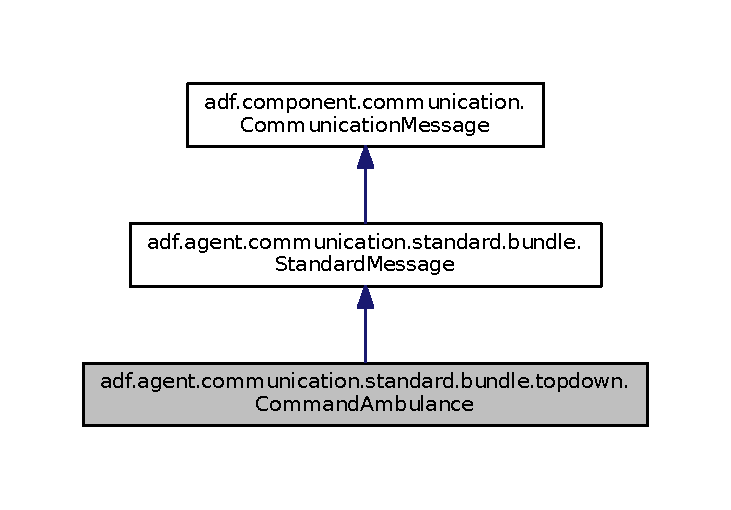
\includegraphics[width=350pt]{classadf_1_1agent_1_1communication_1_1standard_1_1bundle_1_1topdown_1_1CommandAmbulance__inherit__graph}
\end{center}
\end{figure}


Collaboration diagram for adf.\+agent.\+communication.\+standard.\+bundle.\+topdown.\+Command\+Ambulance\+:
\nopagebreak
\begin{figure}[H]
\begin{center}
\leavevmode
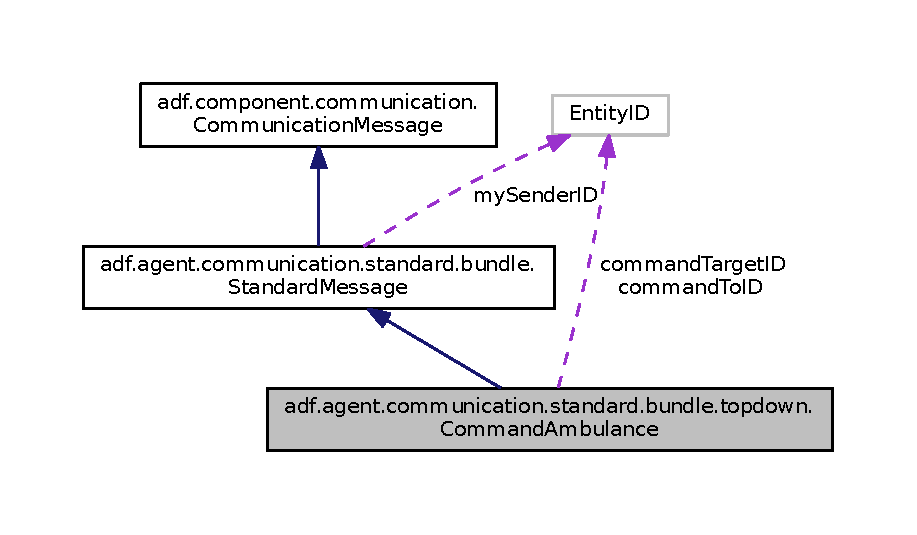
\includegraphics[width=350pt]{classadf_1_1agent_1_1communication_1_1standard_1_1bundle_1_1topdown_1_1CommandAmbulance__coll__graph}
\end{center}
\end{figure}
\subsection*{Public Member Functions}
\begin{DoxyCompactItemize}
\item 
\hypertarget{classadf_1_1agent_1_1communication_1_1standard_1_1bundle_1_1topdown_1_1CommandAmbulance_ad1a27204ff06b816f7ae46e878a5f06d}{}\label{classadf_1_1agent_1_1communication_1_1standard_1_1bundle_1_1topdown_1_1CommandAmbulance_ad1a27204ff06b816f7ae46e878a5f06d} 
{\bfseries Command\+Ambulance} (boolean is\+Radio, Entity\+ID to\+ID, Entity\+ID target\+ID, int action)
\item 
\hypertarget{classadf_1_1agent_1_1communication_1_1standard_1_1bundle_1_1topdown_1_1CommandAmbulance_a2f2920c0847d04bf2436ce93ab97b426}{}\label{classadf_1_1agent_1_1communication_1_1standard_1_1bundle_1_1topdown_1_1CommandAmbulance_a2f2920c0847d04bf2436ce93ab97b426} 
{\bfseries Command\+Ambulance} (boolean is\+Radio, int from, int ttl, \hyperlink{classadf_1_1component_1_1communication_1_1util_1_1BitStreamReader}{Bit\+Stream\+Reader} bit\+Stream\+Reader)
\end{DoxyCompactItemize}
\subsection*{Additional Inherited Members}


\subsection{Detailed Description}
\begin{DoxyRefDesc}{Deprecated}
\item[\hyperlink{deprecated__deprecated000001}{Deprecated}]change class name \hyperlink{classadf_1_1agent_1_1communication_1_1standard_1_1bundle_1_1centralized_1_1CommandAmbulance}{adf.\+agent.\+communication.\+standard.\+bundle.\+centralized.\+Command\+Ambulance} \end{DoxyRefDesc}


The documentation for this class was generated from the following file\+:\begin{DoxyCompactItemize}
\item 
src/main/java/adf/agent/communication/standard/bundle/topdown/Command\+Ambulance.\+java\end{DoxyCompactItemize}

\hypertarget{classadf_1_1agent_1_1communication_1_1standard_1_1bundle_1_1centralized_1_1CommandFire}{}\section{adf.\+agent.\+communication.\+standard.\+bundle.\+centralized.\+Command\+Fire クラス}
\label{classadf_1_1agent_1_1communication_1_1standard_1_1bundle_1_1centralized_1_1CommandFire}\index{adf.\+agent.\+communication.\+standard.\+bundle.\+centralized.\+Command\+Fire@{adf.\+agent.\+communication.\+standard.\+bundle.\+centralized.\+Command\+Fire}}


adf.\+agent.\+communication.\+standard.\+bundle.\+centralized.\+Command\+Fire の継承関係図
\nopagebreak
\begin{figure}[H]
\begin{center}
\leavevmode
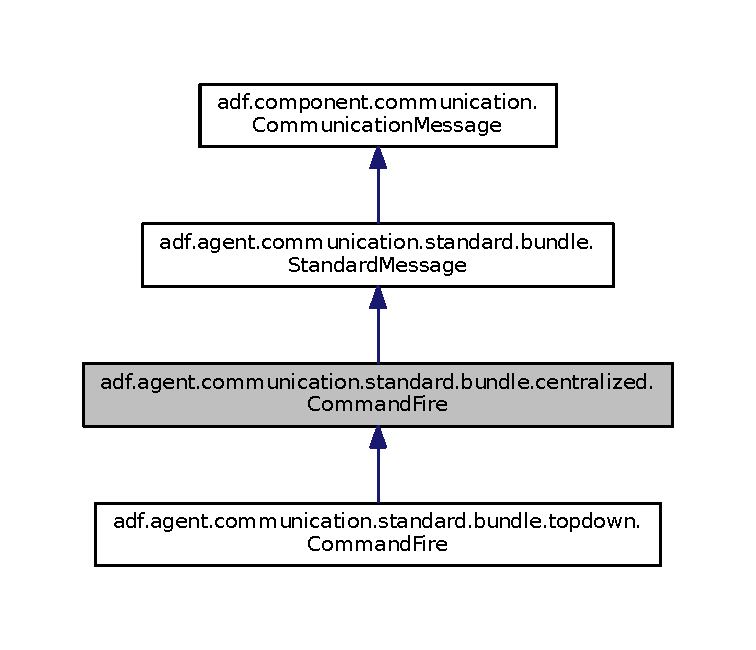
\includegraphics[width=350pt]{classadf_1_1agent_1_1communication_1_1standard_1_1bundle_1_1centralized_1_1CommandFire__inherit__graph}
\end{center}
\end{figure}


adf.\+agent.\+communication.\+standard.\+bundle.\+centralized.\+Command\+Fire 連携図
\nopagebreak
\begin{figure}[H]
\begin{center}
\leavevmode
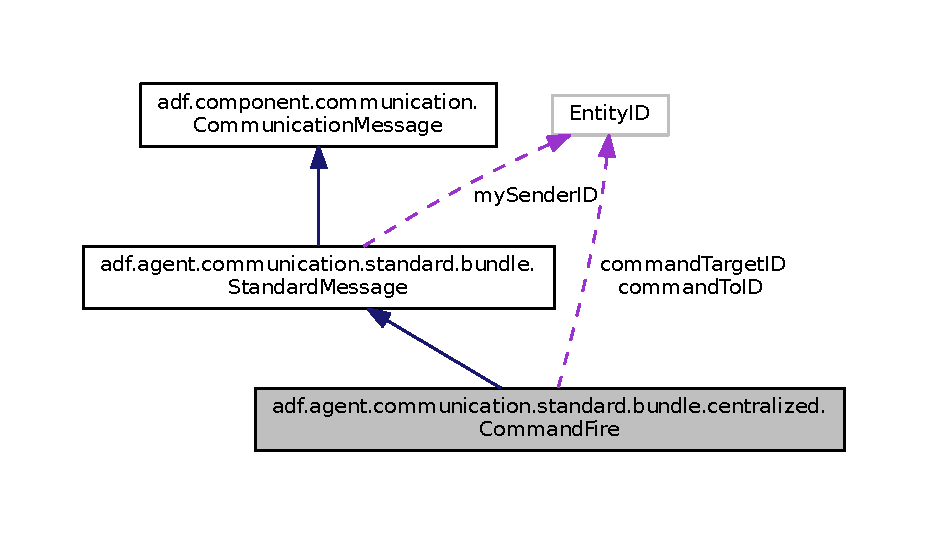
\includegraphics[width=350pt]{classadf_1_1agent_1_1communication_1_1standard_1_1bundle_1_1centralized_1_1CommandFire__coll__graph}
\end{center}
\end{figure}
\subsection*{公開メンバ関数}
\begin{DoxyCompactItemize}
\item 
\hypertarget{classadf_1_1agent_1_1communication_1_1standard_1_1bundle_1_1centralized_1_1CommandFire_a7bae68e663f358632f953822a606a57e}{}\label{classadf_1_1agent_1_1communication_1_1standard_1_1bundle_1_1centralized_1_1CommandFire_a7bae68e663f358632f953822a606a57e} 
{\bfseries Command\+Fire} (boolean is\+Radio, Entity\+ID to\+ID, Entity\+ID target\+ID, int action)
\item 
\hypertarget{classadf_1_1agent_1_1communication_1_1standard_1_1bundle_1_1centralized_1_1CommandFire_a5ff648c1725987c7a6e368b0e62d109a}{}\label{classadf_1_1agent_1_1communication_1_1standard_1_1bundle_1_1centralized_1_1CommandFire_a5ff648c1725987c7a6e368b0e62d109a} 
{\bfseries Command\+Fire} (boolean is\+Radio, int from, int ttl, \hyperlink{classadf_1_1component_1_1communication_1_1util_1_1BitStreamReader}{Bit\+Stream\+Reader} bit\+Stream\+Reader)
\item 
\hypertarget{classadf_1_1agent_1_1communication_1_1standard_1_1bundle_1_1centralized_1_1CommandFire_a622b7ca860cc5f8997344f4a63c226f8}{}\label{classadf_1_1agent_1_1communication_1_1standard_1_1bundle_1_1centralized_1_1CommandFire_a622b7ca860cc5f8997344f4a63c226f8} 
int {\bfseries get\+Action} ()
\item 
\hypertarget{classadf_1_1agent_1_1communication_1_1standard_1_1bundle_1_1centralized_1_1CommandFire_af29ec7c8d3904c6b61473dc4ecf05b13}{}\label{classadf_1_1agent_1_1communication_1_1standard_1_1bundle_1_1centralized_1_1CommandFire_af29ec7c8d3904c6b61473dc4ecf05b13} 
int {\bfseries get\+Byte\+Array\+Size} ()
\item 
\hypertarget{classadf_1_1agent_1_1communication_1_1standard_1_1bundle_1_1centralized_1_1CommandFire_a36bf511b93184bd0e2d272ad89f73932}{}\label{classadf_1_1agent_1_1communication_1_1standard_1_1bundle_1_1centralized_1_1CommandFire_a36bf511b93184bd0e2d272ad89f73932} 
byte \mbox{[}$\,$\mbox{]} {\bfseries to\+Byte\+Array} ()
\item 
\hypertarget{classadf_1_1agent_1_1communication_1_1standard_1_1bundle_1_1centralized_1_1CommandFire_a6f450b71c037caca59472c7695a649af}{}\label{classadf_1_1agent_1_1communication_1_1standard_1_1bundle_1_1centralized_1_1CommandFire_a6f450b71c037caca59472c7695a649af} 
\hyperlink{classadf_1_1component_1_1communication_1_1util_1_1BitOutputStream}{Bit\+Output\+Stream} {\bfseries to\+Bit\+Output\+Stream} ()
\item 
\hypertarget{classadf_1_1agent_1_1communication_1_1standard_1_1bundle_1_1centralized_1_1CommandFire_a55b1f203cac5d536a5a82db03576a090}{}\label{classadf_1_1agent_1_1communication_1_1standard_1_1bundle_1_1centralized_1_1CommandFire_a55b1f203cac5d536a5a82db03576a090} 
Entity\+ID {\bfseries get\+To\+ID} ()
\item 
\hypertarget{classadf_1_1agent_1_1communication_1_1standard_1_1bundle_1_1centralized_1_1CommandFire_a0cf419c3a9a778d7f047323c5cf1fb29}{}\label{classadf_1_1agent_1_1communication_1_1standard_1_1bundle_1_1centralized_1_1CommandFire_a0cf419c3a9a778d7f047323c5cf1fb29} 
Entity\+ID {\bfseries get\+Target\+ID} ()
\item 
\hypertarget{classadf_1_1agent_1_1communication_1_1standard_1_1bundle_1_1centralized_1_1CommandFire_a71ed4d0c0792df132c36ea43b838efb7}{}\label{classadf_1_1agent_1_1communication_1_1standard_1_1bundle_1_1centralized_1_1CommandFire_a71ed4d0c0792df132c36ea43b838efb7} 
boolean {\bfseries is\+Broadcast} ()
\item 
\hypertarget{classadf_1_1agent_1_1communication_1_1standard_1_1bundle_1_1centralized_1_1CommandFire_ae16758957c6dec455931ba33c2a98254}{}\label{classadf_1_1agent_1_1communication_1_1standard_1_1bundle_1_1centralized_1_1CommandFire_ae16758957c6dec455931ba33c2a98254} 
boolean {\bfseries is\+To\+I\+D\+Defined} ()
\item 
\hypertarget{classadf_1_1agent_1_1communication_1_1standard_1_1bundle_1_1centralized_1_1CommandFire_aea13c02c5fea3f93365d0aa03b5e2a2e}{}\label{classadf_1_1agent_1_1communication_1_1standard_1_1bundle_1_1centralized_1_1CommandFire_aea13c02c5fea3f93365d0aa03b5e2a2e} 
boolean {\bfseries id\+Target\+I\+D\+Defined} ()
\item 
\hypertarget{classadf_1_1agent_1_1communication_1_1standard_1_1bundle_1_1centralized_1_1CommandFire_a24a2ac25212c282a08cacdefe221b731}{}\label{classadf_1_1agent_1_1communication_1_1standard_1_1bundle_1_1centralized_1_1CommandFire_a24a2ac25212c282a08cacdefe221b731} 
String {\bfseries get\+Check\+Key} ()
\end{DoxyCompactItemize}
\subsection*{静的公開変数類}
\begin{DoxyCompactItemize}
\item 
\hypertarget{classadf_1_1agent_1_1communication_1_1standard_1_1bundle_1_1centralized_1_1CommandFire_a3b4b9adfb1f3fcab4afe5b5a75b3556f}{}\label{classadf_1_1agent_1_1communication_1_1standard_1_1bundle_1_1centralized_1_1CommandFire_a3b4b9adfb1f3fcab4afe5b5a75b3556f} 
static final int {\bfseries A\+C\+T\+I\+O\+N\+\_\+\+R\+E\+ST} = 0
\item 
\hypertarget{classadf_1_1agent_1_1communication_1_1standard_1_1bundle_1_1centralized_1_1CommandFire_a85a1c34532211f14129a06d1725824c0}{}\label{classadf_1_1agent_1_1communication_1_1standard_1_1bundle_1_1centralized_1_1CommandFire_a85a1c34532211f14129a06d1725824c0} 
static final int {\bfseries A\+C\+T\+I\+O\+N\+\_\+\+M\+O\+VE} = 1
\item 
\hypertarget{classadf_1_1agent_1_1communication_1_1standard_1_1bundle_1_1centralized_1_1CommandFire_a64b7a616876f5accff7a620368586dd7}{}\label{classadf_1_1agent_1_1communication_1_1standard_1_1bundle_1_1centralized_1_1CommandFire_a64b7a616876f5accff7a620368586dd7} 
static final int {\bfseries A\+C\+T\+I\+O\+N\+\_\+\+E\+X\+T\+I\+N\+G\+U\+I\+SH} = 2
\item 
\hypertarget{classadf_1_1agent_1_1communication_1_1standard_1_1bundle_1_1centralized_1_1CommandFire_a785098dee42c7c5d6d452699df5ff87a}{}\label{classadf_1_1agent_1_1communication_1_1standard_1_1bundle_1_1centralized_1_1CommandFire_a785098dee42c7c5d6d452699df5ff87a} 
static final int {\bfseries A\+C\+T\+I\+O\+N\+\_\+\+R\+E\+F\+I\+LL} = 3
\item 
\hypertarget{classadf_1_1agent_1_1communication_1_1standard_1_1bundle_1_1centralized_1_1CommandFire_afdacd2ba6ad3653f1e5e6d4ab0569660}{}\label{classadf_1_1agent_1_1communication_1_1standard_1_1bundle_1_1centralized_1_1CommandFire_afdacd2ba6ad3653f1e5e6d4ab0569660} 
static final int {\bfseries A\+C\+T\+I\+O\+N\+\_\+\+A\+U\+T\+O\+N\+O\+MY} = 4
\end{DoxyCompactItemize}
\subsection*{限定公開変数類}
\begin{DoxyCompactItemize}
\item 
\hypertarget{classadf_1_1agent_1_1communication_1_1standard_1_1bundle_1_1centralized_1_1CommandFire_a82bdd775417bd34a66cdd3ef2f4b6704}{}\label{classadf_1_1agent_1_1communication_1_1standard_1_1bundle_1_1centralized_1_1CommandFire_a82bdd775417bd34a66cdd3ef2f4b6704} 
int {\bfseries raw\+To\+ID}
\item 
\hypertarget{classadf_1_1agent_1_1communication_1_1standard_1_1bundle_1_1centralized_1_1CommandFire_a6f8e1ba3f4e07e275d5a8f1d613d1045}{}\label{classadf_1_1agent_1_1communication_1_1standard_1_1bundle_1_1centralized_1_1CommandFire_a6f8e1ba3f4e07e275d5a8f1d613d1045} 
int {\bfseries raw\+Target\+ID}
\item 
\hypertarget{classadf_1_1agent_1_1communication_1_1standard_1_1bundle_1_1centralized_1_1CommandFire_aaf4e5df81e6cb8aa3ea3b7ba48b3a251}{}\label{classadf_1_1agent_1_1communication_1_1standard_1_1bundle_1_1centralized_1_1CommandFire_aaf4e5df81e6cb8aa3ea3b7ba48b3a251} 
Entity\+ID {\bfseries command\+To\+ID}
\item 
\hypertarget{classadf_1_1agent_1_1communication_1_1standard_1_1bundle_1_1centralized_1_1CommandFire_ae5fce8493a2500b29c7187f495651097}{}\label{classadf_1_1agent_1_1communication_1_1standard_1_1bundle_1_1centralized_1_1CommandFire_ae5fce8493a2500b29c7187f495651097} 
Entity\+ID {\bfseries command\+Target\+ID}
\item 
\hypertarget{classadf_1_1agent_1_1communication_1_1standard_1_1bundle_1_1centralized_1_1CommandFire_a85cbeb2b045c7124c95a2233b67be181}{}\label{classadf_1_1agent_1_1communication_1_1standard_1_1bundle_1_1centralized_1_1CommandFire_a85cbeb2b045c7124c95a2233b67be181} 
int {\bfseries my\+Action}
\item 
\hypertarget{classadf_1_1agent_1_1communication_1_1standard_1_1bundle_1_1centralized_1_1CommandFire_a0bae03d4763b5725247eb7a1dd1a49b0}{}\label{classadf_1_1agent_1_1communication_1_1standard_1_1bundle_1_1centralized_1_1CommandFire_a0bae03d4763b5725247eb7a1dd1a49b0} 
boolean {\bfseries broadcast}
\end{DoxyCompactItemize}
\subsection*{その他の継承メンバ}


このクラス詳解は次のファイルから抽出されました\+:\begin{DoxyCompactItemize}
\item 
src/main/java/adf/agent/communication/standard/bundle/centralized/Command\+Fire.\+java\end{DoxyCompactItemize}

\hypertarget{classadf_1_1agent_1_1communication_1_1standard_1_1bundle_1_1topdown_1_1CommandFire}{}\section{adf.\+agent.\+communication.\+standard.\+bundle.\+topdown.\+Command\+Fire Class Reference}
\label{classadf_1_1agent_1_1communication_1_1standard_1_1bundle_1_1topdown_1_1CommandFire}\index{adf.\+agent.\+communication.\+standard.\+bundle.\+topdown.\+Command\+Fire@{adf.\+agent.\+communication.\+standard.\+bundle.\+topdown.\+Command\+Fire}}


Inheritance diagram for adf.\+agent.\+communication.\+standard.\+bundle.\+topdown.\+Command\+Fire\+:
\nopagebreak
\begin{figure}[H]
\begin{center}
\leavevmode
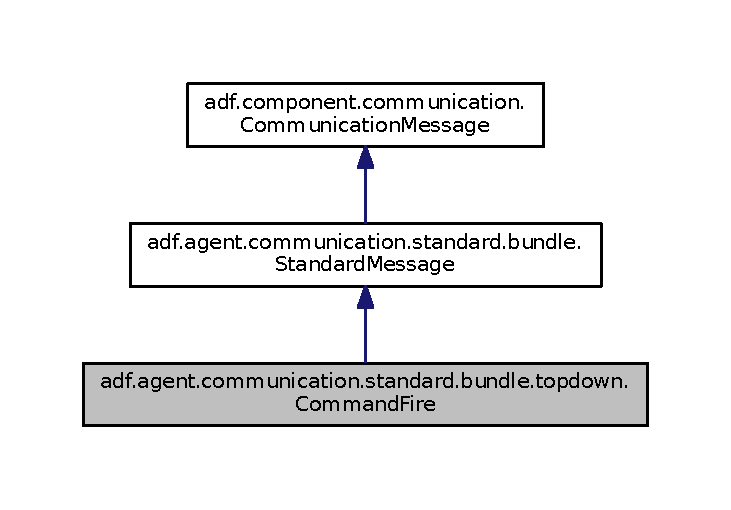
\includegraphics[width=350pt]{classadf_1_1agent_1_1communication_1_1standard_1_1bundle_1_1topdown_1_1CommandFire__inherit__graph}
\end{center}
\end{figure}


Collaboration diagram for adf.\+agent.\+communication.\+standard.\+bundle.\+topdown.\+Command\+Fire\+:
\nopagebreak
\begin{figure}[H]
\begin{center}
\leavevmode
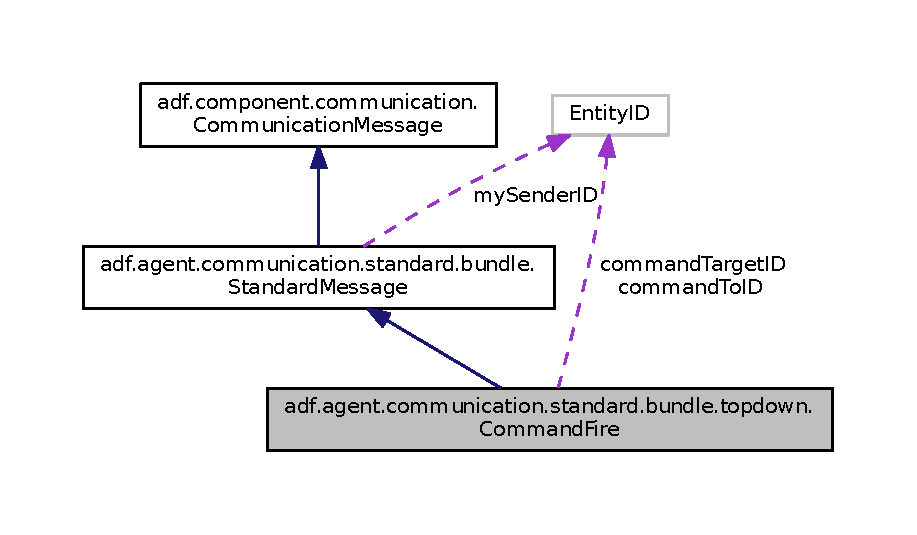
\includegraphics[width=350pt]{classadf_1_1agent_1_1communication_1_1standard_1_1bundle_1_1topdown_1_1CommandFire__coll__graph}
\end{center}
\end{figure}
\subsection*{Public Member Functions}
\begin{DoxyCompactItemize}
\item 
\hypertarget{classadf_1_1agent_1_1communication_1_1standard_1_1bundle_1_1topdown_1_1CommandFire_a096f6d1f59e59d3e50d4aaa81627ffe5}{}\label{classadf_1_1agent_1_1communication_1_1standard_1_1bundle_1_1topdown_1_1CommandFire_a096f6d1f59e59d3e50d4aaa81627ffe5} 
{\bfseries Command\+Fire} (boolean is\+Radio, Entity\+ID to\+ID, Entity\+ID target\+ID, int action)
\item 
\hypertarget{classadf_1_1agent_1_1communication_1_1standard_1_1bundle_1_1topdown_1_1CommandFire_a7a3979249cfbe7491fcb6a25ba3b7260}{}\label{classadf_1_1agent_1_1communication_1_1standard_1_1bundle_1_1topdown_1_1CommandFire_a7a3979249cfbe7491fcb6a25ba3b7260} 
{\bfseries Command\+Fire} (boolean is\+Radio, int from, int ttl, \hyperlink{classadf_1_1component_1_1communication_1_1util_1_1BitStreamReader}{Bit\+Stream\+Reader} bit\+Stream\+Reader)
\item 
\hypertarget{classadf_1_1agent_1_1communication_1_1standard_1_1bundle_1_1topdown_1_1CommandFire_ac5b6f3774aba7df932872d62aa5a4562}{}\label{classadf_1_1agent_1_1communication_1_1standard_1_1bundle_1_1topdown_1_1CommandFire_ac5b6f3774aba7df932872d62aa5a4562} 
int {\bfseries get\+Action} ()
\item 
\hypertarget{classadf_1_1agent_1_1communication_1_1standard_1_1bundle_1_1topdown_1_1CommandFire_a31d8677dededcf55229510bb013d4258}{}\label{classadf_1_1agent_1_1communication_1_1standard_1_1bundle_1_1topdown_1_1CommandFire_a31d8677dededcf55229510bb013d4258} 
int {\bfseries get\+Byte\+Array\+Size} ()
\item 
\hypertarget{classadf_1_1agent_1_1communication_1_1standard_1_1bundle_1_1topdown_1_1CommandFire_abbcfbbd10848d3ec6d5ed0ce3f6074c0}{}\label{classadf_1_1agent_1_1communication_1_1standard_1_1bundle_1_1topdown_1_1CommandFire_abbcfbbd10848d3ec6d5ed0ce3f6074c0} 
byte \mbox{[}$\,$\mbox{]} {\bfseries to\+Byte\+Array} ()
\item 
\hypertarget{classadf_1_1agent_1_1communication_1_1standard_1_1bundle_1_1topdown_1_1CommandFire_a4e69239f9f8c5c6ad6b381ac5eff2ded}{}\label{classadf_1_1agent_1_1communication_1_1standard_1_1bundle_1_1topdown_1_1CommandFire_a4e69239f9f8c5c6ad6b381ac5eff2ded} 
\hyperlink{classadf_1_1component_1_1communication_1_1util_1_1BitOutputStream}{Bit\+Output\+Stream} {\bfseries to\+Bit\+Output\+Stream} ()
\item 
\hypertarget{classadf_1_1agent_1_1communication_1_1standard_1_1bundle_1_1topdown_1_1CommandFire_adb3cb9e159a47538991a500f14d51f0b}{}\label{classadf_1_1agent_1_1communication_1_1standard_1_1bundle_1_1topdown_1_1CommandFire_adb3cb9e159a47538991a500f14d51f0b} 
Entity\+ID {\bfseries get\+To\+ID} ()
\item 
\hypertarget{classadf_1_1agent_1_1communication_1_1standard_1_1bundle_1_1topdown_1_1CommandFire_a0d725d91651495d7fefeb312c8443a2c}{}\label{classadf_1_1agent_1_1communication_1_1standard_1_1bundle_1_1topdown_1_1CommandFire_a0d725d91651495d7fefeb312c8443a2c} 
Entity\+ID {\bfseries get\+Target\+ID} ()
\item 
\hypertarget{classadf_1_1agent_1_1communication_1_1standard_1_1bundle_1_1topdown_1_1CommandFire_a3c841a9e8543da9a57c2dc9903349c66}{}\label{classadf_1_1agent_1_1communication_1_1standard_1_1bundle_1_1topdown_1_1CommandFire_a3c841a9e8543da9a57c2dc9903349c66} 
boolean {\bfseries is\+Broadcast} ()
\item 
\hypertarget{classadf_1_1agent_1_1communication_1_1standard_1_1bundle_1_1topdown_1_1CommandFire_a85e4e0b77c8901962666720b4cabef1a}{}\label{classadf_1_1agent_1_1communication_1_1standard_1_1bundle_1_1topdown_1_1CommandFire_a85e4e0b77c8901962666720b4cabef1a} 
boolean {\bfseries is\+To\+I\+D\+Defined} ()
\item 
\hypertarget{classadf_1_1agent_1_1communication_1_1standard_1_1bundle_1_1topdown_1_1CommandFire_a11a8ac924f389dc27e1efb306095a523}{}\label{classadf_1_1agent_1_1communication_1_1standard_1_1bundle_1_1topdown_1_1CommandFire_a11a8ac924f389dc27e1efb306095a523} 
boolean {\bfseries id\+Target\+I\+D\+Defined} ()
\item 
\hypertarget{classadf_1_1agent_1_1communication_1_1standard_1_1bundle_1_1topdown_1_1CommandFire_a366306e02bfd89c87453fef3e93fe0b9}{}\label{classadf_1_1agent_1_1communication_1_1standard_1_1bundle_1_1topdown_1_1CommandFire_a366306e02bfd89c87453fef3e93fe0b9} 
String {\bfseries get\+Check\+Key} ()
\end{DoxyCompactItemize}
\subsection*{Static Public Attributes}
\begin{DoxyCompactItemize}
\item 
\hypertarget{classadf_1_1agent_1_1communication_1_1standard_1_1bundle_1_1topdown_1_1CommandFire_afa30f4a1fcc31ddf5508245f4797308e}{}\label{classadf_1_1agent_1_1communication_1_1standard_1_1bundle_1_1topdown_1_1CommandFire_afa30f4a1fcc31ddf5508245f4797308e} 
static final int {\bfseries A\+C\+T\+I\+O\+N\+\_\+\+R\+E\+ST} = 0
\item 
\hypertarget{classadf_1_1agent_1_1communication_1_1standard_1_1bundle_1_1topdown_1_1CommandFire_aad0e2973f1765b7468dd331ba9d1cf30}{}\label{classadf_1_1agent_1_1communication_1_1standard_1_1bundle_1_1topdown_1_1CommandFire_aad0e2973f1765b7468dd331ba9d1cf30} 
static final int {\bfseries A\+C\+T\+I\+O\+N\+\_\+\+M\+O\+VE} = 1
\item 
\hypertarget{classadf_1_1agent_1_1communication_1_1standard_1_1bundle_1_1topdown_1_1CommandFire_ad86049025937c32d2e171f6768de4fc2}{}\label{classadf_1_1agent_1_1communication_1_1standard_1_1bundle_1_1topdown_1_1CommandFire_ad86049025937c32d2e171f6768de4fc2} 
static final int {\bfseries A\+C\+T\+I\+O\+N\+\_\+\+E\+X\+T\+I\+N\+G\+U\+I\+SH} = 2
\item 
\hypertarget{classadf_1_1agent_1_1communication_1_1standard_1_1bundle_1_1topdown_1_1CommandFire_a63aa837d7ae63197772b029b6bf7ace8}{}\label{classadf_1_1agent_1_1communication_1_1standard_1_1bundle_1_1topdown_1_1CommandFire_a63aa837d7ae63197772b029b6bf7ace8} 
static final int {\bfseries A\+C\+T\+I\+O\+N\+\_\+\+R\+E\+F\+I\+LL} = 3
\end{DoxyCompactItemize}
\subsection*{Protected Attributes}
\begin{DoxyCompactItemize}
\item 
\hypertarget{classadf_1_1agent_1_1communication_1_1standard_1_1bundle_1_1topdown_1_1CommandFire_a9dc1206054fe357c2d4f70f56ed4317d}{}\label{classadf_1_1agent_1_1communication_1_1standard_1_1bundle_1_1topdown_1_1CommandFire_a9dc1206054fe357c2d4f70f56ed4317d} 
int {\bfseries raw\+To\+ID}
\item 
\hypertarget{classadf_1_1agent_1_1communication_1_1standard_1_1bundle_1_1topdown_1_1CommandFire_a0aa5fc09c19fca117a0f56ecff606e9b}{}\label{classadf_1_1agent_1_1communication_1_1standard_1_1bundle_1_1topdown_1_1CommandFire_a0aa5fc09c19fca117a0f56ecff606e9b} 
int {\bfseries raw\+Target\+ID}
\item 
\hypertarget{classadf_1_1agent_1_1communication_1_1standard_1_1bundle_1_1topdown_1_1CommandFire_a7638a069bac5b762afe9124c052b5e56}{}\label{classadf_1_1agent_1_1communication_1_1standard_1_1bundle_1_1topdown_1_1CommandFire_a7638a069bac5b762afe9124c052b5e56} 
Entity\+ID {\bfseries command\+To\+ID}
\item 
\hypertarget{classadf_1_1agent_1_1communication_1_1standard_1_1bundle_1_1topdown_1_1CommandFire_abfb8caea8fbc5dee3b0369e74fdb4be6}{}\label{classadf_1_1agent_1_1communication_1_1standard_1_1bundle_1_1topdown_1_1CommandFire_abfb8caea8fbc5dee3b0369e74fdb4be6} 
Entity\+ID {\bfseries command\+Target\+ID}
\item 
\hypertarget{classadf_1_1agent_1_1communication_1_1standard_1_1bundle_1_1topdown_1_1CommandFire_a37ec07982370fe310434d3b50d368b8a}{}\label{classadf_1_1agent_1_1communication_1_1standard_1_1bundle_1_1topdown_1_1CommandFire_a37ec07982370fe310434d3b50d368b8a} 
int {\bfseries my\+Action}
\item 
\hypertarget{classadf_1_1agent_1_1communication_1_1standard_1_1bundle_1_1topdown_1_1CommandFire_a46eb557d1d645390bc21d02676adbd59}{}\label{classadf_1_1agent_1_1communication_1_1standard_1_1bundle_1_1topdown_1_1CommandFire_a46eb557d1d645390bc21d02676adbd59} 
boolean {\bfseries broadcast}
\end{DoxyCompactItemize}
\subsection*{Additional Inherited Members}


The documentation for this class was generated from the following file\+:\begin{DoxyCompactItemize}
\item 
src/main/java/adf/agent/communication/standard/bundle/topdown/Command\+Fire.\+java\end{DoxyCompactItemize}

\hypertarget{classadf_1_1component_1_1command_1_1CommandGenerator}{}\section{adf.\+component.\+command.\+Command\+Generator Class Reference}
\label{classadf_1_1component_1_1command_1_1CommandGenerator}\index{adf.\+component.\+command.\+Command\+Generator@{adf.\+component.\+command.\+Command\+Generator}}


Collaboration diagram for adf.\+component.\+command.\+Command\+Generator\+:
\nopagebreak
\begin{figure}[H]
\begin{center}
\leavevmode
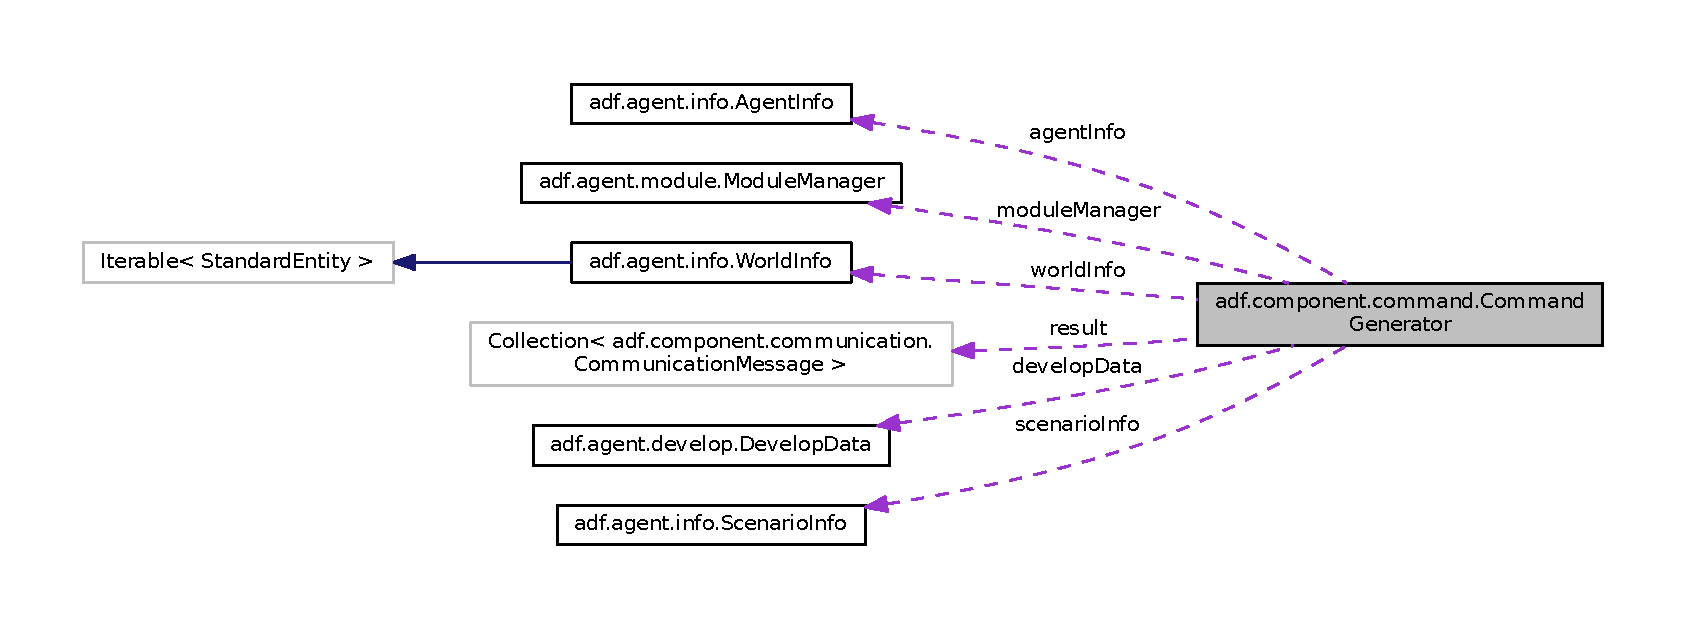
\includegraphics[width=350pt]{classadf_1_1component_1_1command_1_1CommandGenerator__coll__graph}
\end{center}
\end{figure}
\subsection*{Public Member Functions}
\begin{DoxyCompactItemize}
\item 
\hypertarget{classadf_1_1component_1_1command_1_1CommandGenerator_a579e876e1447a86dd950db6d810c6d07}{}\label{classadf_1_1component_1_1command_1_1CommandGenerator_a579e876e1447a86dd950db6d810c6d07} 
{\bfseries Command\+Generator} (\hyperlink{classadf_1_1agent_1_1info_1_1AgentInfo}{Agent\+Info} ai, \hyperlink{classadf_1_1agent_1_1info_1_1WorldInfo}{World\+Info} wi, \hyperlink{classadf_1_1agent_1_1info_1_1ScenarioInfo}{Scenario\+Info} si, \hyperlink{classadf_1_1agent_1_1module_1_1ModuleManager}{Module\+Manager} module\+Manager, \hyperlink{classadf_1_1agent_1_1develop_1_1DevelopData}{Develop\+Data} develop\+Data)
\item 
\hypertarget{classadf_1_1component_1_1command_1_1CommandGenerator_a61589fda1263d0062286cd4b04c013d3}{}\label{classadf_1_1component_1_1command_1_1CommandGenerator_a61589fda1263d0062286cd4b04c013d3} 
abstract \hyperlink{classadf_1_1component_1_1command_1_1CommandGenerator}{Command\+Generator} {\bfseries set\+Data} (Map$<$ Entity\+ID, Entity\+ID $>$ allocation\+Data)
\item 
\hypertarget{classadf_1_1component_1_1command_1_1CommandGenerator_ad454eb64f15bce3eb1e5661815f36476}{}\label{classadf_1_1component_1_1command_1_1CommandGenerator_ad454eb64f15bce3eb1e5661815f36476} 
Collection$<$ \hyperlink{classadf_1_1component_1_1communication_1_1CommunicationMessage}{Communication\+Message} $>$ {\bfseries get\+Result} ()
\item 
\hypertarget{classadf_1_1component_1_1command_1_1CommandGenerator_a713b9d5d2e15bfe2bc2c28d80ad0c4cb}{}\label{classadf_1_1component_1_1command_1_1CommandGenerator_a713b9d5d2e15bfe2bc2c28d80ad0c4cb} 
\hyperlink{classadf_1_1component_1_1command_1_1CommandGenerator}{Command\+Generator} {\bfseries precompute} (\hyperlink{classadf_1_1agent_1_1precompute_1_1PrecomputeData}{Precompute\+Data} precompute\+Data)
\item 
\hypertarget{classadf_1_1component_1_1command_1_1CommandGenerator_a2fbfbc00ee2234b3769ab3160dab4b9c}{}\label{classadf_1_1component_1_1command_1_1CommandGenerator_a2fbfbc00ee2234b3769ab3160dab4b9c} 
\hyperlink{classadf_1_1component_1_1command_1_1CommandGenerator}{Command\+Generator} {\bfseries resume} (\hyperlink{classadf_1_1agent_1_1precompute_1_1PrecomputeData}{Precompute\+Data} precompute\+Data)
\item 
\hypertarget{classadf_1_1component_1_1command_1_1CommandGenerator_aa2ab31b2efe2a69e1b0cdb89307ba2d5}{}\label{classadf_1_1component_1_1command_1_1CommandGenerator_aa2ab31b2efe2a69e1b0cdb89307ba2d5} 
\hyperlink{classadf_1_1component_1_1command_1_1CommandGenerator}{Command\+Generator} {\bfseries preparate} ()
\item 
\hypertarget{classadf_1_1component_1_1command_1_1CommandGenerator_a14b257fa2988e8e44d51bac2f6f3a5fc}{}\label{classadf_1_1component_1_1command_1_1CommandGenerator_a14b257fa2988e8e44d51bac2f6f3a5fc} 
\hyperlink{classadf_1_1component_1_1command_1_1CommandGenerator}{Command\+Generator} {\bfseries update\+Info} (\hyperlink{classadf_1_1agent_1_1communication_1_1MessageManager}{Message\+Manager} message\+Manager)
\item 
\hypertarget{classadf_1_1component_1_1command_1_1CommandGenerator_ae6e194bcec75cff40c427cc7ece619c3}{}\label{classadf_1_1component_1_1command_1_1CommandGenerator_ae6e194bcec75cff40c427cc7ece619c3} 
int {\bfseries get\+Count\+Precompute} ()
\item 
\hypertarget{classadf_1_1component_1_1command_1_1CommandGenerator_a77ec8cae118f0d7e7ffff6df3c842d8b}{}\label{classadf_1_1component_1_1command_1_1CommandGenerator_a77ec8cae118f0d7e7ffff6df3c842d8b} 
int {\bfseries get\+Count\+Resume} ()
\item 
\hypertarget{classadf_1_1component_1_1command_1_1CommandGenerator_a42075303fd034ffc65b444de8c7d3154}{}\label{classadf_1_1component_1_1command_1_1CommandGenerator_a42075303fd034ffc65b444de8c7d3154} 
int {\bfseries get\+Count\+Preparate} ()
\item 
\hypertarget{classadf_1_1component_1_1command_1_1CommandGenerator_a25e01c383e24f7ec09190bcaf1313dec}{}\label{classadf_1_1component_1_1command_1_1CommandGenerator_a25e01c383e24f7ec09190bcaf1313dec} 
int {\bfseries get\+Count\+Update\+Info} ()
\item 
\hypertarget{classadf_1_1component_1_1command_1_1CommandGenerator_a1fe8126306bfe9df5edb1947e4c0abae}{}\label{classadf_1_1component_1_1command_1_1CommandGenerator_a1fe8126306bfe9df5edb1947e4c0abae} 
void {\bfseries reset\+Count\+Precompute} ()
\item 
\hypertarget{classadf_1_1component_1_1command_1_1CommandGenerator_ac15d08b0d27a142d5ee86f9595ee37c2}{}\label{classadf_1_1component_1_1command_1_1CommandGenerator_ac15d08b0d27a142d5ee86f9595ee37c2} 
void {\bfseries reset\+Count\+Resume} ()
\item 
\hypertarget{classadf_1_1component_1_1command_1_1CommandGenerator_a4e90c7dc90e34174f8ad8da76bde85e9}{}\label{classadf_1_1component_1_1command_1_1CommandGenerator_a4e90c7dc90e34174f8ad8da76bde85e9} 
void {\bfseries reset\+Count\+Preparate} ()
\item 
\hypertarget{classadf_1_1component_1_1command_1_1CommandGenerator_a11042e27effecc3cc82e2af5e1df1b7a}{}\label{classadf_1_1component_1_1command_1_1CommandGenerator_a11042e27effecc3cc82e2af5e1df1b7a} 
void {\bfseries reset\+Count\+Update\+Info} ()
\end{DoxyCompactItemize}
\subsection*{Protected Attributes}
\begin{DoxyCompactItemize}
\item 
\hypertarget{classadf_1_1component_1_1command_1_1CommandGenerator_a543633658836fd35a1a84863a6590db1}{}\label{classadf_1_1component_1_1command_1_1CommandGenerator_a543633658836fd35a1a84863a6590db1} 
\hyperlink{classadf_1_1agent_1_1info_1_1ScenarioInfo}{Scenario\+Info} {\bfseries scenario\+Info}
\item 
\hypertarget{classadf_1_1component_1_1command_1_1CommandGenerator_a8d7f44b456637032255eacd51e8cfc27}{}\label{classadf_1_1component_1_1command_1_1CommandGenerator_a8d7f44b456637032255eacd51e8cfc27} 
\hyperlink{classadf_1_1agent_1_1info_1_1AgentInfo}{Agent\+Info} {\bfseries agent\+Info}
\item 
\hypertarget{classadf_1_1component_1_1command_1_1CommandGenerator_ac0f8b8c16c071a23223d7485cd188c97}{}\label{classadf_1_1component_1_1command_1_1CommandGenerator_ac0f8b8c16c071a23223d7485cd188c97} 
\hyperlink{classadf_1_1agent_1_1info_1_1WorldInfo}{World\+Info} {\bfseries world\+Info}
\item 
\hypertarget{classadf_1_1component_1_1command_1_1CommandGenerator_ab10faeffe7d6547cf5d27726c64a699d}{}\label{classadf_1_1component_1_1command_1_1CommandGenerator_ab10faeffe7d6547cf5d27726c64a699d} 
\hyperlink{classadf_1_1agent_1_1module_1_1ModuleManager}{Module\+Manager} {\bfseries module\+Manager}
\item 
\hypertarget{classadf_1_1component_1_1command_1_1CommandGenerator_adce137b57368269f73e5259b0f844279}{}\label{classadf_1_1component_1_1command_1_1CommandGenerator_adce137b57368269f73e5259b0f844279} 
\hyperlink{classadf_1_1agent_1_1develop_1_1DevelopData}{Develop\+Data} {\bfseries develop\+Data}
\item 
\hypertarget{classadf_1_1component_1_1command_1_1CommandGenerator_a60302b470fa7607d888d5545ea17d311}{}\label{classadf_1_1component_1_1command_1_1CommandGenerator_a60302b470fa7607d888d5545ea17d311} 
Collection$<$ \hyperlink{classadf_1_1component_1_1communication_1_1CommunicationMessage}{Communication\+Message} $>$ {\bfseries result}
\end{DoxyCompactItemize}


The documentation for this class was generated from the following file\+:\begin{DoxyCompactItemize}
\item 
src/main/java/adf/component/command/Command\+Generator.\+java\end{DoxyCompactItemize}

\hypertarget{classadf_1_1agent_1_1communication_1_1standard_1_1bundle_1_1centralized_1_1CommandPolice}{}\section{adf.\+agent.\+communication.\+standard.\+bundle.\+centralized.\+Command\+Police Class Reference}
\label{classadf_1_1agent_1_1communication_1_1standard_1_1bundle_1_1centralized_1_1CommandPolice}\index{adf.\+agent.\+communication.\+standard.\+bundle.\+centralized.\+Command\+Police@{adf.\+agent.\+communication.\+standard.\+bundle.\+centralized.\+Command\+Police}}


Inheritance diagram for adf.\+agent.\+communication.\+standard.\+bundle.\+centralized.\+Command\+Police\+:
\nopagebreak
\begin{figure}[H]
\begin{center}
\leavevmode
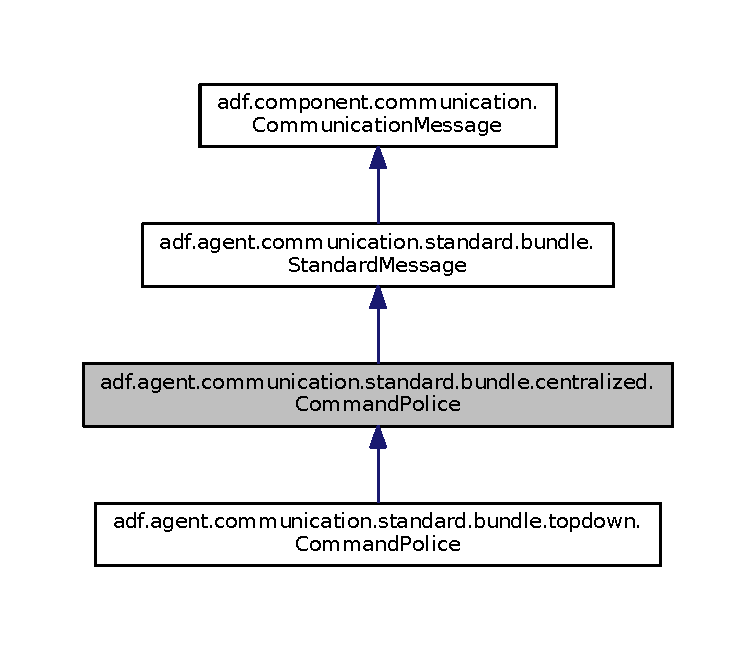
\includegraphics[width=350pt]{classadf_1_1agent_1_1communication_1_1standard_1_1bundle_1_1centralized_1_1CommandPolice__inherit__graph}
\end{center}
\end{figure}


Collaboration diagram for adf.\+agent.\+communication.\+standard.\+bundle.\+centralized.\+Command\+Police\+:
\nopagebreak
\begin{figure}[H]
\begin{center}
\leavevmode
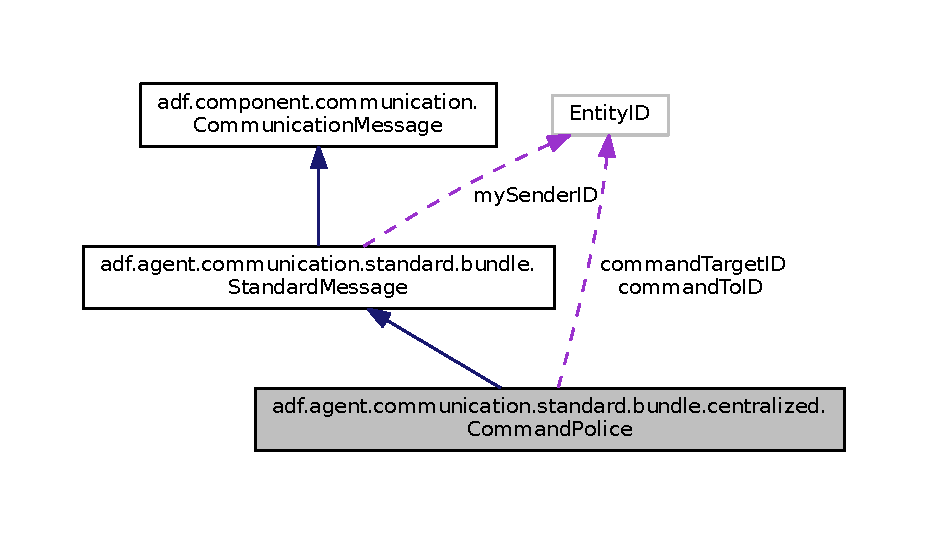
\includegraphics[width=350pt]{classadf_1_1agent_1_1communication_1_1standard_1_1bundle_1_1centralized_1_1CommandPolice__coll__graph}
\end{center}
\end{figure}
\subsection*{Public Member Functions}
\begin{DoxyCompactItemize}
\item 
\hypertarget{classadf_1_1agent_1_1communication_1_1standard_1_1bundle_1_1centralized_1_1CommandPolice_ac747822b23d13b000beb3b87899123a1}{}\label{classadf_1_1agent_1_1communication_1_1standard_1_1bundle_1_1centralized_1_1CommandPolice_ac747822b23d13b000beb3b87899123a1} 
{\bfseries Command\+Police} (boolean is\+Radio, Entity\+ID to\+ID, Entity\+ID target\+ID, int action)
\item 
\hypertarget{classadf_1_1agent_1_1communication_1_1standard_1_1bundle_1_1centralized_1_1CommandPolice_ae700d27dad6fa5ee05fa26f99b61e26e}{}\label{classadf_1_1agent_1_1communication_1_1standard_1_1bundle_1_1centralized_1_1CommandPolice_ae700d27dad6fa5ee05fa26f99b61e26e} 
{\bfseries Command\+Police} (boolean is\+Radio, int from, int ttl, \hyperlink{classadf_1_1component_1_1communication_1_1util_1_1BitStreamReader}{Bit\+Stream\+Reader} bit\+Stream\+Reader)
\item 
\hypertarget{classadf_1_1agent_1_1communication_1_1standard_1_1bundle_1_1centralized_1_1CommandPolice_a0460d50153618a65c5a39253c7947ec3}{}\label{classadf_1_1agent_1_1communication_1_1standard_1_1bundle_1_1centralized_1_1CommandPolice_a0460d50153618a65c5a39253c7947ec3} 
int {\bfseries get\+Action} ()
\item 
\hypertarget{classadf_1_1agent_1_1communication_1_1standard_1_1bundle_1_1centralized_1_1CommandPolice_aaa4419097722ca8e6296e9c943bb9bdc}{}\label{classadf_1_1agent_1_1communication_1_1standard_1_1bundle_1_1centralized_1_1CommandPolice_aaa4419097722ca8e6296e9c943bb9bdc} 
int {\bfseries get\+Byte\+Array\+Size} ()
\item 
\hypertarget{classadf_1_1agent_1_1communication_1_1standard_1_1bundle_1_1centralized_1_1CommandPolice_ae3b054102b803bfc346cc0eb3c2a5e67}{}\label{classadf_1_1agent_1_1communication_1_1standard_1_1bundle_1_1centralized_1_1CommandPolice_ae3b054102b803bfc346cc0eb3c2a5e67} 
byte \mbox{[}$\,$\mbox{]} {\bfseries to\+Byte\+Array} ()
\item 
\hypertarget{classadf_1_1agent_1_1communication_1_1standard_1_1bundle_1_1centralized_1_1CommandPolice_a989a2862919a4f61ece93dd21668b1fd}{}\label{classadf_1_1agent_1_1communication_1_1standard_1_1bundle_1_1centralized_1_1CommandPolice_a989a2862919a4f61ece93dd21668b1fd} 
\hyperlink{classadf_1_1component_1_1communication_1_1util_1_1BitOutputStream}{Bit\+Output\+Stream} {\bfseries to\+Bit\+Output\+Stream} ()
\item 
\hypertarget{classadf_1_1agent_1_1communication_1_1standard_1_1bundle_1_1centralized_1_1CommandPolice_aa7721bd28a714278f4b6ffb032ecd4ac}{}\label{classadf_1_1agent_1_1communication_1_1standard_1_1bundle_1_1centralized_1_1CommandPolice_aa7721bd28a714278f4b6ffb032ecd4ac} 
Entity\+ID {\bfseries get\+To\+ID} ()
\item 
\hypertarget{classadf_1_1agent_1_1communication_1_1standard_1_1bundle_1_1centralized_1_1CommandPolice_a77fdd0308dd7b781a8fbd7538e0f2d5f}{}\label{classadf_1_1agent_1_1communication_1_1standard_1_1bundle_1_1centralized_1_1CommandPolice_a77fdd0308dd7b781a8fbd7538e0f2d5f} 
Entity\+ID {\bfseries get\+Target\+ID} ()
\item 
\hypertarget{classadf_1_1agent_1_1communication_1_1standard_1_1bundle_1_1centralized_1_1CommandPolice_a9fae7de0f67e860f676fea5e365d8b67}{}\label{classadf_1_1agent_1_1communication_1_1standard_1_1bundle_1_1centralized_1_1CommandPolice_a9fae7de0f67e860f676fea5e365d8b67} 
boolean {\bfseries is\+Broadcast} ()
\item 
\hypertarget{classadf_1_1agent_1_1communication_1_1standard_1_1bundle_1_1centralized_1_1CommandPolice_a65da1e834c95a3a3df2fb39de5418b35}{}\label{classadf_1_1agent_1_1communication_1_1standard_1_1bundle_1_1centralized_1_1CommandPolice_a65da1e834c95a3a3df2fb39de5418b35} 
boolean {\bfseries is\+To\+I\+D\+Defined} ()
\item 
\hypertarget{classadf_1_1agent_1_1communication_1_1standard_1_1bundle_1_1centralized_1_1CommandPolice_af29111fbcf18fdfffef22c57aef4a835}{}\label{classadf_1_1agent_1_1communication_1_1standard_1_1bundle_1_1centralized_1_1CommandPolice_af29111fbcf18fdfffef22c57aef4a835} 
boolean {\bfseries id\+Target\+I\+D\+Defined} ()
\item 
\hypertarget{classadf_1_1agent_1_1communication_1_1standard_1_1bundle_1_1centralized_1_1CommandPolice_a2ad3546787db886dad63fb032dcb8f17}{}\label{classadf_1_1agent_1_1communication_1_1standard_1_1bundle_1_1centralized_1_1CommandPolice_a2ad3546787db886dad63fb032dcb8f17} 
String {\bfseries get\+Check\+Key} ()
\end{DoxyCompactItemize}
\subsection*{Static Public Attributes}
\begin{DoxyCompactItemize}
\item 
\hypertarget{classadf_1_1agent_1_1communication_1_1standard_1_1bundle_1_1centralized_1_1CommandPolice_aaf2390128f6b732903b62012de3a84a5}{}\label{classadf_1_1agent_1_1communication_1_1standard_1_1bundle_1_1centralized_1_1CommandPolice_aaf2390128f6b732903b62012de3a84a5} 
static final int {\bfseries A\+C\+T\+I\+O\+N\+\_\+\+R\+E\+ST} = 0
\item 
\hypertarget{classadf_1_1agent_1_1communication_1_1standard_1_1bundle_1_1centralized_1_1CommandPolice_a93482f8b25fafb93657db32327751b8e}{}\label{classadf_1_1agent_1_1communication_1_1standard_1_1bundle_1_1centralized_1_1CommandPolice_a93482f8b25fafb93657db32327751b8e} 
static final int {\bfseries A\+C\+T\+I\+O\+N\+\_\+\+M\+O\+VE} = 1
\item 
\hypertarget{classadf_1_1agent_1_1communication_1_1standard_1_1bundle_1_1centralized_1_1CommandPolice_a78b408d996c0739c389c929b454643d9}{}\label{classadf_1_1agent_1_1communication_1_1standard_1_1bundle_1_1centralized_1_1CommandPolice_a78b408d996c0739c389c929b454643d9} 
static final int {\bfseries A\+C\+T\+I\+O\+N\+\_\+\+C\+L\+E\+AR} = 2
\item 
\hypertarget{classadf_1_1agent_1_1communication_1_1standard_1_1bundle_1_1centralized_1_1CommandPolice_a724f43d40368fde30c95363738eeb77e}{}\label{classadf_1_1agent_1_1communication_1_1standard_1_1bundle_1_1centralized_1_1CommandPolice_a724f43d40368fde30c95363738eeb77e} 
static final int {\bfseries A\+C\+T\+I\+O\+N\+\_\+\+A\+U\+T\+O\+N\+O\+MY} = 3
\end{DoxyCompactItemize}
\subsection*{Protected Attributes}
\begin{DoxyCompactItemize}
\item 
\hypertarget{classadf_1_1agent_1_1communication_1_1standard_1_1bundle_1_1centralized_1_1CommandPolice_ae8c679d636a28ae546a9f4181ddf6100}{}\label{classadf_1_1agent_1_1communication_1_1standard_1_1bundle_1_1centralized_1_1CommandPolice_ae8c679d636a28ae546a9f4181ddf6100} 
int {\bfseries raw\+To\+ID}
\item 
\hypertarget{classadf_1_1agent_1_1communication_1_1standard_1_1bundle_1_1centralized_1_1CommandPolice_aae55db1875805499e98740b6d38d5ed3}{}\label{classadf_1_1agent_1_1communication_1_1standard_1_1bundle_1_1centralized_1_1CommandPolice_aae55db1875805499e98740b6d38d5ed3} 
int {\bfseries raw\+Target\+ID}
\item 
\hypertarget{classadf_1_1agent_1_1communication_1_1standard_1_1bundle_1_1centralized_1_1CommandPolice_a0c1b7caf001436ad3ba26c4913c63a46}{}\label{classadf_1_1agent_1_1communication_1_1standard_1_1bundle_1_1centralized_1_1CommandPolice_a0c1b7caf001436ad3ba26c4913c63a46} 
Entity\+ID {\bfseries command\+To\+ID}
\item 
\hypertarget{classadf_1_1agent_1_1communication_1_1standard_1_1bundle_1_1centralized_1_1CommandPolice_ae0925f1844cdb9a019c309b3972fa399}{}\label{classadf_1_1agent_1_1communication_1_1standard_1_1bundle_1_1centralized_1_1CommandPolice_ae0925f1844cdb9a019c309b3972fa399} 
Entity\+ID {\bfseries command\+Target\+ID}
\item 
\hypertarget{classadf_1_1agent_1_1communication_1_1standard_1_1bundle_1_1centralized_1_1CommandPolice_ac4959c130aef15079efd18fc62d03bba}{}\label{classadf_1_1agent_1_1communication_1_1standard_1_1bundle_1_1centralized_1_1CommandPolice_ac4959c130aef15079efd18fc62d03bba} 
int {\bfseries my\+Action}
\item 
\hypertarget{classadf_1_1agent_1_1communication_1_1standard_1_1bundle_1_1centralized_1_1CommandPolice_a5c5bec5e7a73480cefa5cb83524db8ff}{}\label{classadf_1_1agent_1_1communication_1_1standard_1_1bundle_1_1centralized_1_1CommandPolice_a5c5bec5e7a73480cefa5cb83524db8ff} 
boolean {\bfseries broadcast}
\end{DoxyCompactItemize}
\subsection*{Additional Inherited Members}


The documentation for this class was generated from the following file\+:\begin{DoxyCompactItemize}
\item 
src/main/java/adf/agent/communication/standard/bundle/centralized/Command\+Police.\+java\end{DoxyCompactItemize}

\hypertarget{classadf_1_1agent_1_1communication_1_1standard_1_1bundle_1_1topdown_1_1CommandPolice}{}\section{adf.\+agent.\+communication.\+standard.\+bundle.\+topdown.\+Command\+Police クラス}
\label{classadf_1_1agent_1_1communication_1_1standard_1_1bundle_1_1topdown_1_1CommandPolice}\index{adf.\+agent.\+communication.\+standard.\+bundle.\+topdown.\+Command\+Police@{adf.\+agent.\+communication.\+standard.\+bundle.\+topdown.\+Command\+Police}}


adf.\+agent.\+communication.\+standard.\+bundle.\+topdown.\+Command\+Police の継承関係図
\nopagebreak
\begin{figure}[H]
\begin{center}
\leavevmode
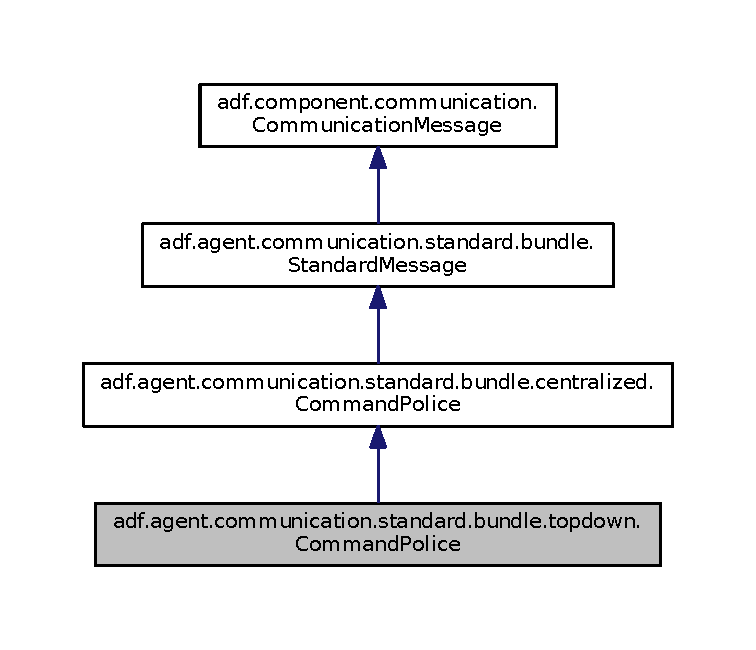
\includegraphics[width=350pt]{classadf_1_1agent_1_1communication_1_1standard_1_1bundle_1_1topdown_1_1CommandPolice__inherit__graph}
\end{center}
\end{figure}


adf.\+agent.\+communication.\+standard.\+bundle.\+topdown.\+Command\+Police 連携図
\nopagebreak
\begin{figure}[H]
\begin{center}
\leavevmode
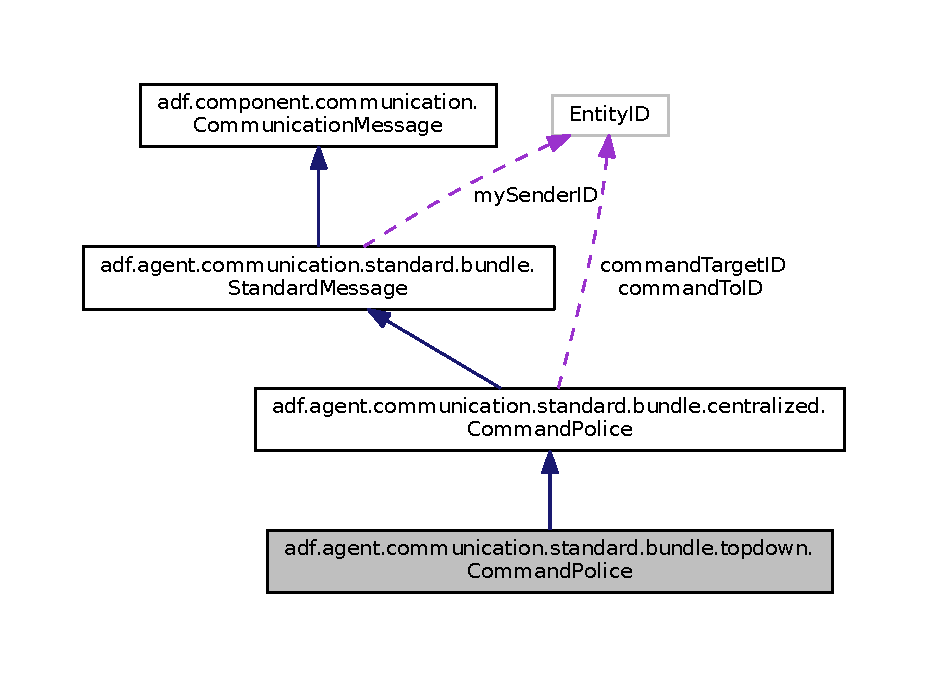
\includegraphics[width=350pt]{classadf_1_1agent_1_1communication_1_1standard_1_1bundle_1_1topdown_1_1CommandPolice__coll__graph}
\end{center}
\end{figure}
\subsection*{公開メンバ関数}
\begin{DoxyCompactItemize}
\item 
\hypertarget{classadf_1_1agent_1_1communication_1_1standard_1_1bundle_1_1topdown_1_1CommandPolice_aa8cda9c94c7876cbd37c15925411aa23}{}\label{classadf_1_1agent_1_1communication_1_1standard_1_1bundle_1_1topdown_1_1CommandPolice_aa8cda9c94c7876cbd37c15925411aa23} 
{\bfseries Command\+Police} (boolean is\+Radio, Entity\+ID to\+ID, Entity\+ID target\+ID, int action)
\item 
\hypertarget{classadf_1_1agent_1_1communication_1_1standard_1_1bundle_1_1topdown_1_1CommandPolice_afdeb2bff9db87a9436ffb6171a437a16}{}\label{classadf_1_1agent_1_1communication_1_1standard_1_1bundle_1_1topdown_1_1CommandPolice_afdeb2bff9db87a9436ffb6171a437a16} 
{\bfseries Command\+Police} (boolean is\+Radio, int from, int ttl, \hyperlink{classadf_1_1component_1_1communication_1_1util_1_1BitStreamReader}{Bit\+Stream\+Reader} bit\+Stream\+Reader)
\item 
\hypertarget{classadf_1_1agent_1_1communication_1_1standard_1_1bundle_1_1topdown_1_1CommandPolice_a7abd4a426513be758360db96ced6954a}{}\label{classadf_1_1agent_1_1communication_1_1standard_1_1bundle_1_1topdown_1_1CommandPolice_a7abd4a426513be758360db96ced6954a} 
int {\bfseries get\+Action} ()
\item 
\hypertarget{classadf_1_1agent_1_1communication_1_1standard_1_1bundle_1_1topdown_1_1CommandPolice_a3e547d0aee9c3f35fee95f9c7de9b70e}{}\label{classadf_1_1agent_1_1communication_1_1standard_1_1bundle_1_1topdown_1_1CommandPolice_a3e547d0aee9c3f35fee95f9c7de9b70e} 
int {\bfseries get\+Byte\+Array\+Size} ()
\item 
\hypertarget{classadf_1_1agent_1_1communication_1_1standard_1_1bundle_1_1topdown_1_1CommandPolice_a57f726945e1cf968a6c82433f8b39cf9}{}\label{classadf_1_1agent_1_1communication_1_1standard_1_1bundle_1_1topdown_1_1CommandPolice_a57f726945e1cf968a6c82433f8b39cf9} 
byte \mbox{[}$\,$\mbox{]} {\bfseries to\+Byte\+Array} ()
\item 
\hypertarget{classadf_1_1agent_1_1communication_1_1standard_1_1bundle_1_1topdown_1_1CommandPolice_a750351c36ad0e796ab59d528ef7a8e03}{}\label{classadf_1_1agent_1_1communication_1_1standard_1_1bundle_1_1topdown_1_1CommandPolice_a750351c36ad0e796ab59d528ef7a8e03} 
\hyperlink{classadf_1_1component_1_1communication_1_1util_1_1BitOutputStream}{Bit\+Output\+Stream} {\bfseries to\+Bit\+Output\+Stream} ()
\item 
\hypertarget{classadf_1_1agent_1_1communication_1_1standard_1_1bundle_1_1topdown_1_1CommandPolice_a8767df49e8e3645146229fa86b2e713c}{}\label{classadf_1_1agent_1_1communication_1_1standard_1_1bundle_1_1topdown_1_1CommandPolice_a8767df49e8e3645146229fa86b2e713c} 
Entity\+ID {\bfseries get\+To\+ID} ()
\item 
\hypertarget{classadf_1_1agent_1_1communication_1_1standard_1_1bundle_1_1topdown_1_1CommandPolice_a92b4ada5f71adbf896339a62f07c14e5}{}\label{classadf_1_1agent_1_1communication_1_1standard_1_1bundle_1_1topdown_1_1CommandPolice_a92b4ada5f71adbf896339a62f07c14e5} 
Entity\+ID {\bfseries get\+Target\+ID} ()
\item 
\hypertarget{classadf_1_1agent_1_1communication_1_1standard_1_1bundle_1_1topdown_1_1CommandPolice_a252219e67363b18c9e59dabd1e2c3e3a}{}\label{classadf_1_1agent_1_1communication_1_1standard_1_1bundle_1_1topdown_1_1CommandPolice_a252219e67363b18c9e59dabd1e2c3e3a} 
boolean {\bfseries is\+Broadcast} ()
\item 
\hypertarget{classadf_1_1agent_1_1communication_1_1standard_1_1bundle_1_1topdown_1_1CommandPolice_a01f0202568db91faec7c0b2ea795ebb3}{}\label{classadf_1_1agent_1_1communication_1_1standard_1_1bundle_1_1topdown_1_1CommandPolice_a01f0202568db91faec7c0b2ea795ebb3} 
boolean {\bfseries is\+To\+I\+D\+Defined} ()
\item 
\hypertarget{classadf_1_1agent_1_1communication_1_1standard_1_1bundle_1_1topdown_1_1CommandPolice_acc6a4aea98674e9163f3a3e2e7c77fdd}{}\label{classadf_1_1agent_1_1communication_1_1standard_1_1bundle_1_1topdown_1_1CommandPolice_acc6a4aea98674e9163f3a3e2e7c77fdd} 
boolean {\bfseries id\+Target\+I\+D\+Defined} ()
\item 
\hypertarget{classadf_1_1agent_1_1communication_1_1standard_1_1bundle_1_1topdown_1_1CommandPolice_aaccece77cd25d8791d0f29f56516b088}{}\label{classadf_1_1agent_1_1communication_1_1standard_1_1bundle_1_1topdown_1_1CommandPolice_aaccece77cd25d8791d0f29f56516b088} 
String {\bfseries get\+Check\+Key} ()
\end{DoxyCompactItemize}
\subsection*{静的公開変数類}
\begin{DoxyCompactItemize}
\item 
\hypertarget{classadf_1_1agent_1_1communication_1_1standard_1_1bundle_1_1topdown_1_1CommandPolice_a8e6207452651cbd469fbd2d0003a24e8}{}\label{classadf_1_1agent_1_1communication_1_1standard_1_1bundle_1_1topdown_1_1CommandPolice_a8e6207452651cbd469fbd2d0003a24e8} 
static final int {\bfseries A\+C\+T\+I\+O\+N\+\_\+\+R\+E\+ST} = 0
\item 
\hypertarget{classadf_1_1agent_1_1communication_1_1standard_1_1bundle_1_1topdown_1_1CommandPolice_aa26dbdd850218675c283dff686df32e1}{}\label{classadf_1_1agent_1_1communication_1_1standard_1_1bundle_1_1topdown_1_1CommandPolice_aa26dbdd850218675c283dff686df32e1} 
static final int {\bfseries A\+C\+T\+I\+O\+N\+\_\+\+M\+O\+VE} = 1
\item 
\hypertarget{classadf_1_1agent_1_1communication_1_1standard_1_1bundle_1_1topdown_1_1CommandPolice_a11afae15bfe26c40649e76e3068deec6}{}\label{classadf_1_1agent_1_1communication_1_1standard_1_1bundle_1_1topdown_1_1CommandPolice_a11afae15bfe26c40649e76e3068deec6} 
static final int {\bfseries A\+C\+T\+I\+O\+N\+\_\+\+C\+L\+E\+AR} = 2
\end{DoxyCompactItemize}
\subsection*{限定公開変数類}
\begin{DoxyCompactItemize}
\item 
\hypertarget{classadf_1_1agent_1_1communication_1_1standard_1_1bundle_1_1topdown_1_1CommandPolice_aa780239e05d4eee72bba2f010e0cf37f}{}\label{classadf_1_1agent_1_1communication_1_1standard_1_1bundle_1_1topdown_1_1CommandPolice_aa780239e05d4eee72bba2f010e0cf37f} 
int {\bfseries raw\+To\+ID}
\item 
\hypertarget{classadf_1_1agent_1_1communication_1_1standard_1_1bundle_1_1topdown_1_1CommandPolice_ab4e2a31bc7ac624425ae083eb4510a3f}{}\label{classadf_1_1agent_1_1communication_1_1standard_1_1bundle_1_1topdown_1_1CommandPolice_ab4e2a31bc7ac624425ae083eb4510a3f} 
int {\bfseries raw\+Target\+ID}
\item 
\hypertarget{classadf_1_1agent_1_1communication_1_1standard_1_1bundle_1_1topdown_1_1CommandPolice_af555844ae2ce52d127f2b83304b012a0}{}\label{classadf_1_1agent_1_1communication_1_1standard_1_1bundle_1_1topdown_1_1CommandPolice_af555844ae2ce52d127f2b83304b012a0} 
Entity\+ID {\bfseries command\+To\+ID}
\item 
\hypertarget{classadf_1_1agent_1_1communication_1_1standard_1_1bundle_1_1topdown_1_1CommandPolice_a17f5e43f5dd4772899e4bd26977932a9}{}\label{classadf_1_1agent_1_1communication_1_1standard_1_1bundle_1_1topdown_1_1CommandPolice_a17f5e43f5dd4772899e4bd26977932a9} 
Entity\+ID {\bfseries command\+Target\+ID}
\item 
\hypertarget{classadf_1_1agent_1_1communication_1_1standard_1_1bundle_1_1topdown_1_1CommandPolice_a1226fb13b11a2b7164e265d76d48cabf}{}\label{classadf_1_1agent_1_1communication_1_1standard_1_1bundle_1_1topdown_1_1CommandPolice_a1226fb13b11a2b7164e265d76d48cabf} 
int {\bfseries my\+Action}
\item 
\hypertarget{classadf_1_1agent_1_1communication_1_1standard_1_1bundle_1_1topdown_1_1CommandPolice_a15e8dd86eff2eb8035edf18910d387c6}{}\label{classadf_1_1agent_1_1communication_1_1standard_1_1bundle_1_1topdown_1_1CommandPolice_a15e8dd86eff2eb8035edf18910d387c6} 
boolean {\bfseries broadcast}
\end{DoxyCompactItemize}
\subsection*{その他の継承メンバ}


このクラス詳解は次のファイルから抽出されました\+:\begin{DoxyCompactItemize}
\item 
src/main/java/adf/agent/communication/standard/bundle/topdown/Command\+Police.\+java\end{DoxyCompactItemize}

\hypertarget{classadf_1_1agent_1_1communication_1_1standard_1_1bundle_1_1centralized_1_1CommandScout}{}\section{adf.\+agent.\+communication.\+standard.\+bundle.\+centralized.\+Command\+Scout クラス}
\label{classadf_1_1agent_1_1communication_1_1standard_1_1bundle_1_1centralized_1_1CommandScout}\index{adf.\+agent.\+communication.\+standard.\+bundle.\+centralized.\+Command\+Scout@{adf.\+agent.\+communication.\+standard.\+bundle.\+centralized.\+Command\+Scout}}


adf.\+agent.\+communication.\+standard.\+bundle.\+centralized.\+Command\+Scout の継承関係図
\nopagebreak
\begin{figure}[H]
\begin{center}
\leavevmode
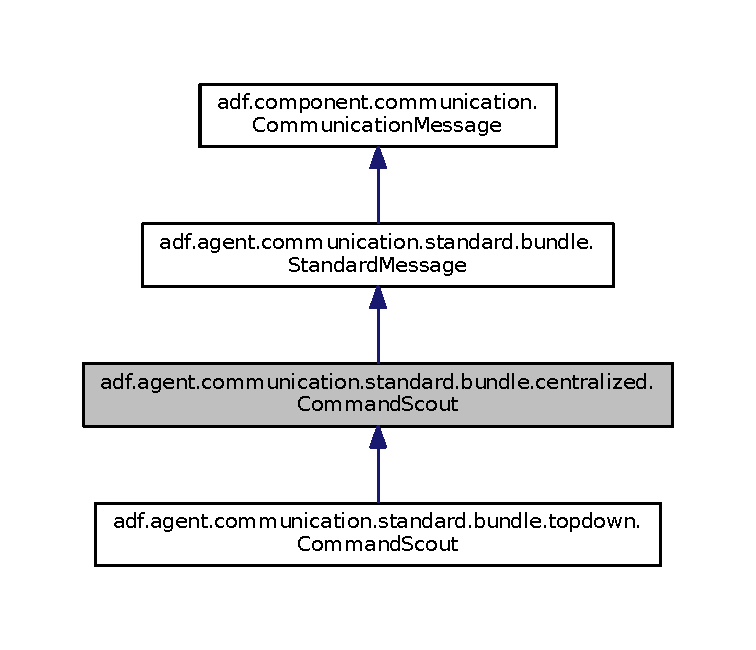
\includegraphics[width=350pt]{classadf_1_1agent_1_1communication_1_1standard_1_1bundle_1_1centralized_1_1CommandScout__inherit__graph}
\end{center}
\end{figure}


adf.\+agent.\+communication.\+standard.\+bundle.\+centralized.\+Command\+Scout 連携図
\nopagebreak
\begin{figure}[H]
\begin{center}
\leavevmode
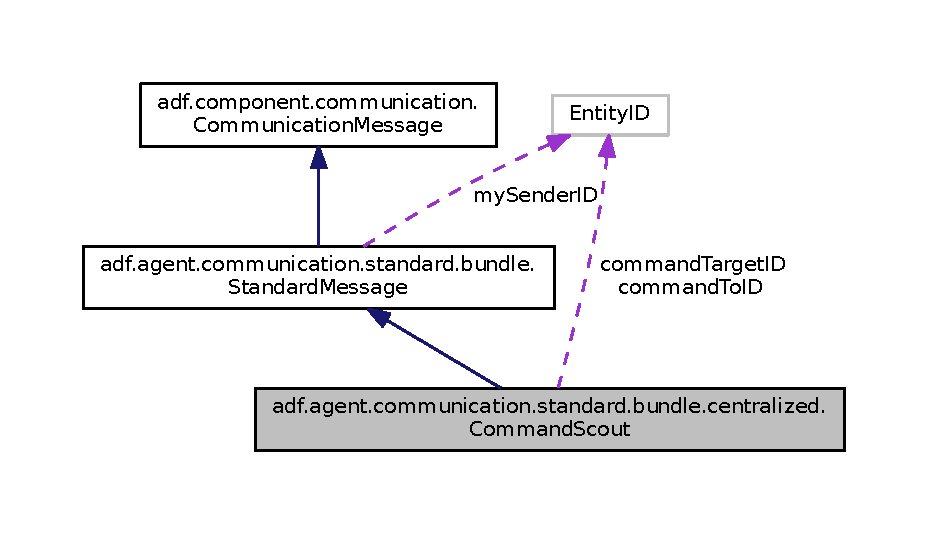
\includegraphics[width=350pt]{classadf_1_1agent_1_1communication_1_1standard_1_1bundle_1_1centralized_1_1CommandScout__coll__graph}
\end{center}
\end{figure}
\subsection*{公開メンバ関数}
\begin{DoxyCompactItemize}
\item 
\hypertarget{classadf_1_1agent_1_1communication_1_1standard_1_1bundle_1_1centralized_1_1CommandScout_aff9ecd70669b3eb58531cd57c32d8555}{}\label{classadf_1_1agent_1_1communication_1_1standard_1_1bundle_1_1centralized_1_1CommandScout_aff9ecd70669b3eb58531cd57c32d8555} 
{\bfseries Command\+Scout} (boolean is\+Radio, Entity\+ID to\+ID, Entity\+ID target\+ID, int range)
\item 
\hypertarget{classadf_1_1agent_1_1communication_1_1standard_1_1bundle_1_1centralized_1_1CommandScout_ac9a91440db6b74364862aee281528f82}{}\label{classadf_1_1agent_1_1communication_1_1standard_1_1bundle_1_1centralized_1_1CommandScout_ac9a91440db6b74364862aee281528f82} 
{\bfseries Command\+Scout} (boolean is\+Radio, int from, int ttl, \hyperlink{classadf_1_1component_1_1communication_1_1util_1_1BitStreamReader}{Bit\+Stream\+Reader} bit\+Stream\+Reader)
\item 
\hypertarget{classadf_1_1agent_1_1communication_1_1standard_1_1bundle_1_1centralized_1_1CommandScout_ae77d422cb3e3fe1fffa6c80a8eb5e7c8}{}\label{classadf_1_1agent_1_1communication_1_1standard_1_1bundle_1_1centralized_1_1CommandScout_ae77d422cb3e3fe1fffa6c80a8eb5e7c8} 
int {\bfseries get\+Range} ()
\item 
\hypertarget{classadf_1_1agent_1_1communication_1_1standard_1_1bundle_1_1centralized_1_1CommandScout_a4627c3fe6e6d80533db053eba19a5f29}{}\label{classadf_1_1agent_1_1communication_1_1standard_1_1bundle_1_1centralized_1_1CommandScout_a4627c3fe6e6d80533db053eba19a5f29} 
int {\bfseries get\+Byte\+Array\+Size} ()
\item 
\hypertarget{classadf_1_1agent_1_1communication_1_1standard_1_1bundle_1_1centralized_1_1CommandScout_a68460d46dad6b559d17a70f08b2ec114}{}\label{classadf_1_1agent_1_1communication_1_1standard_1_1bundle_1_1centralized_1_1CommandScout_a68460d46dad6b559d17a70f08b2ec114} 
byte \mbox{[}$\,$\mbox{]} {\bfseries to\+Byte\+Array} ()
\item 
\hypertarget{classadf_1_1agent_1_1communication_1_1standard_1_1bundle_1_1centralized_1_1CommandScout_a02d53c2c9125cea7714fadf97b2614ba}{}\label{classadf_1_1agent_1_1communication_1_1standard_1_1bundle_1_1centralized_1_1CommandScout_a02d53c2c9125cea7714fadf97b2614ba} 
\hyperlink{classadf_1_1component_1_1communication_1_1util_1_1BitOutputStream}{Bit\+Output\+Stream} {\bfseries to\+Bit\+Output\+Stream} ()
\item 
\hypertarget{classadf_1_1agent_1_1communication_1_1standard_1_1bundle_1_1centralized_1_1CommandScout_aba6cdf24324621bee5707642744a5c28}{}\label{classadf_1_1agent_1_1communication_1_1standard_1_1bundle_1_1centralized_1_1CommandScout_aba6cdf24324621bee5707642744a5c28} 
Entity\+ID {\bfseries get\+To\+ID} ()
\item 
\hypertarget{classadf_1_1agent_1_1communication_1_1standard_1_1bundle_1_1centralized_1_1CommandScout_a5d74241313af1073be2dbe5d51f2cf11}{}\label{classadf_1_1agent_1_1communication_1_1standard_1_1bundle_1_1centralized_1_1CommandScout_a5d74241313af1073be2dbe5d51f2cf11} 
Entity\+ID {\bfseries get\+Target\+ID} ()
\item 
\hypertarget{classadf_1_1agent_1_1communication_1_1standard_1_1bundle_1_1centralized_1_1CommandScout_a683345368cd228744f32910d1085e15e}{}\label{classadf_1_1agent_1_1communication_1_1standard_1_1bundle_1_1centralized_1_1CommandScout_a683345368cd228744f32910d1085e15e} 
boolean {\bfseries is\+Broadcast} ()
\item 
\hypertarget{classadf_1_1agent_1_1communication_1_1standard_1_1bundle_1_1centralized_1_1CommandScout_acdd637cd8b62ecd35d912934f2cec344}{}\label{classadf_1_1agent_1_1communication_1_1standard_1_1bundle_1_1centralized_1_1CommandScout_acdd637cd8b62ecd35d912934f2cec344} 
boolean {\bfseries is\+To\+I\+D\+Defined} ()
\item 
\hypertarget{classadf_1_1agent_1_1communication_1_1standard_1_1bundle_1_1centralized_1_1CommandScout_a643c1671e4c5bb8e88f9efc3faa58260}{}\label{classadf_1_1agent_1_1communication_1_1standard_1_1bundle_1_1centralized_1_1CommandScout_a643c1671e4c5bb8e88f9efc3faa58260} 
boolean {\bfseries id\+Target\+I\+D\+Defined} ()
\item 
\hypertarget{classadf_1_1agent_1_1communication_1_1standard_1_1bundle_1_1centralized_1_1CommandScout_afb63ecc3b605895a101ef94183774816}{}\label{classadf_1_1agent_1_1communication_1_1standard_1_1bundle_1_1centralized_1_1CommandScout_afb63ecc3b605895a101ef94183774816} 
String {\bfseries get\+Check\+Key} ()
\end{DoxyCompactItemize}
\subsection*{限定公開変数類}
\begin{DoxyCompactItemize}
\item 
\hypertarget{classadf_1_1agent_1_1communication_1_1standard_1_1bundle_1_1centralized_1_1CommandScout_a1f60975ba8efdff7cd14d27b15f5df79}{}\label{classadf_1_1agent_1_1communication_1_1standard_1_1bundle_1_1centralized_1_1CommandScout_a1f60975ba8efdff7cd14d27b15f5df79} 
int {\bfseries raw\+To\+ID}
\item 
\hypertarget{classadf_1_1agent_1_1communication_1_1standard_1_1bundle_1_1centralized_1_1CommandScout_a83a07a8511379eab334bb2acf99c19f2}{}\label{classadf_1_1agent_1_1communication_1_1standard_1_1bundle_1_1centralized_1_1CommandScout_a83a07a8511379eab334bb2acf99c19f2} 
int {\bfseries raw\+Target\+ID}
\item 
\hypertarget{classadf_1_1agent_1_1communication_1_1standard_1_1bundle_1_1centralized_1_1CommandScout_a02ec990c0adfac132a48a2b0b637b1ca}{}\label{classadf_1_1agent_1_1communication_1_1standard_1_1bundle_1_1centralized_1_1CommandScout_a02ec990c0adfac132a48a2b0b637b1ca} 
Entity\+ID {\bfseries command\+To\+ID}
\item 
\hypertarget{classadf_1_1agent_1_1communication_1_1standard_1_1bundle_1_1centralized_1_1CommandScout_ac064c242a5757c9e4063391192ca1f0e}{}\label{classadf_1_1agent_1_1communication_1_1standard_1_1bundle_1_1centralized_1_1CommandScout_ac064c242a5757c9e4063391192ca1f0e} 
Entity\+ID {\bfseries command\+Target\+ID}
\item 
\hypertarget{classadf_1_1agent_1_1communication_1_1standard_1_1bundle_1_1centralized_1_1CommandScout_a9378ee2673497c99bda86473501ea9b1}{}\label{classadf_1_1agent_1_1communication_1_1standard_1_1bundle_1_1centralized_1_1CommandScout_a9378ee2673497c99bda86473501ea9b1} 
int {\bfseries scout\+Range}
\item 
\hypertarget{classadf_1_1agent_1_1communication_1_1standard_1_1bundle_1_1centralized_1_1CommandScout_a5b36747655353d8ac8db0c6d81893baf}{}\label{classadf_1_1agent_1_1communication_1_1standard_1_1bundle_1_1centralized_1_1CommandScout_a5b36747655353d8ac8db0c6d81893baf} 
boolean {\bfseries broadcast}
\end{DoxyCompactItemize}
\subsection*{その他の継承メンバ}


このクラス詳解は次のファイルから抽出されました\+:\begin{DoxyCompactItemize}
\item 
src/main/java/adf/agent/communication/standard/bundle/centralized/Command\+Scout.\+java\end{DoxyCompactItemize}

\hypertarget{classadf_1_1agent_1_1communication_1_1standard_1_1bundle_1_1topdown_1_1CommandScout}{}\section{adf.\+agent.\+communication.\+standard.\+bundle.\+topdown.\+Command\+Scout Class Reference}
\label{classadf_1_1agent_1_1communication_1_1standard_1_1bundle_1_1topdown_1_1CommandScout}\index{adf.\+agent.\+communication.\+standard.\+bundle.\+topdown.\+Command\+Scout@{adf.\+agent.\+communication.\+standard.\+bundle.\+topdown.\+Command\+Scout}}


Inheritance diagram for adf.\+agent.\+communication.\+standard.\+bundle.\+topdown.\+Command\+Scout\+:
\nopagebreak
\begin{figure}[H]
\begin{center}
\leavevmode
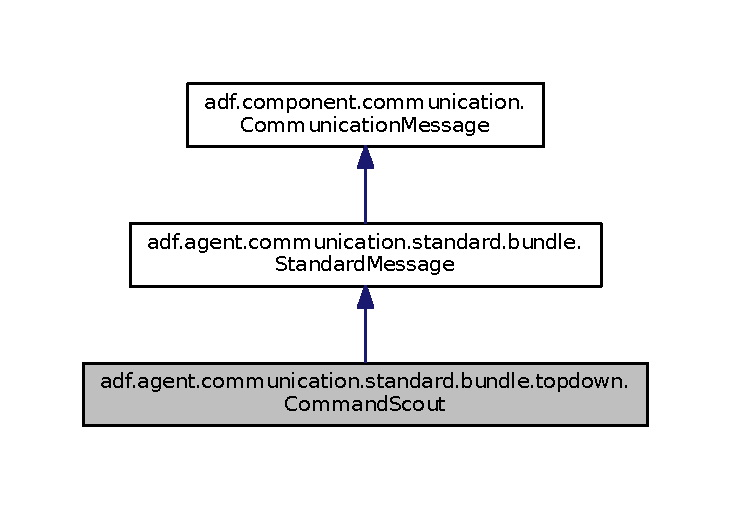
\includegraphics[width=350pt]{classadf_1_1agent_1_1communication_1_1standard_1_1bundle_1_1topdown_1_1CommandScout__inherit__graph}
\end{center}
\end{figure}


Collaboration diagram for adf.\+agent.\+communication.\+standard.\+bundle.\+topdown.\+Command\+Scout\+:
\nopagebreak
\begin{figure}[H]
\begin{center}
\leavevmode
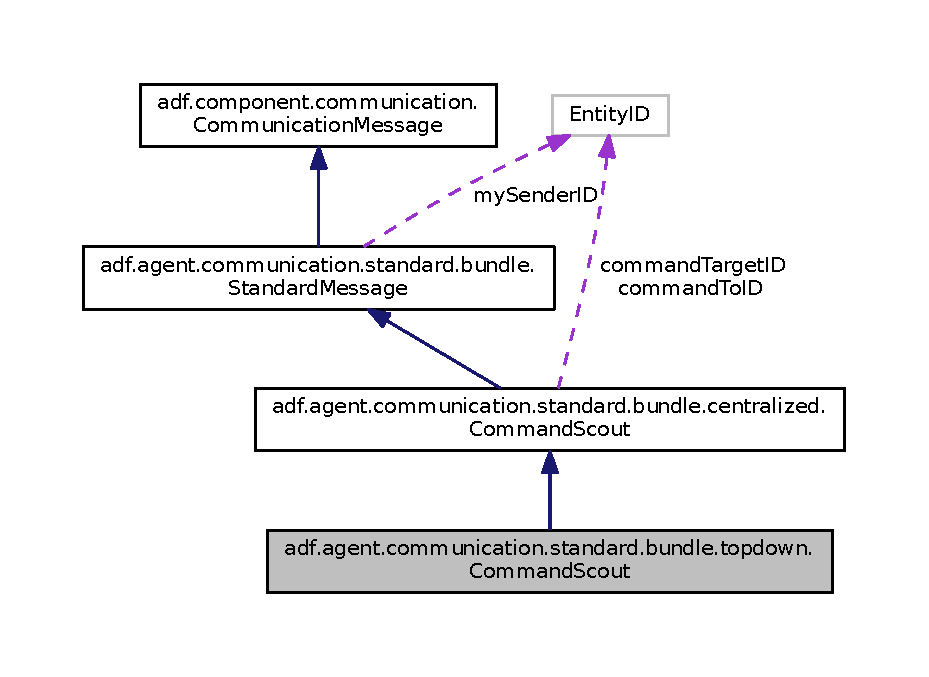
\includegraphics[width=350pt]{classadf_1_1agent_1_1communication_1_1standard_1_1bundle_1_1topdown_1_1CommandScout__coll__graph}
\end{center}
\end{figure}
\subsection*{Public Member Functions}
\begin{DoxyCompactItemize}
\item 
\hypertarget{classadf_1_1agent_1_1communication_1_1standard_1_1bundle_1_1topdown_1_1CommandScout_ac0a0110b57ef6dbb1974ce6162860868}{}\label{classadf_1_1agent_1_1communication_1_1standard_1_1bundle_1_1topdown_1_1CommandScout_ac0a0110b57ef6dbb1974ce6162860868} 
{\bfseries Command\+Scout} (boolean is\+Radio, Entity\+ID to\+ID, Entity\+ID target\+ID, int range)
\item 
\hypertarget{classadf_1_1agent_1_1communication_1_1standard_1_1bundle_1_1topdown_1_1CommandScout_acdf95a514aa45b155b08d4b250343c9b}{}\label{classadf_1_1agent_1_1communication_1_1standard_1_1bundle_1_1topdown_1_1CommandScout_acdf95a514aa45b155b08d4b250343c9b} 
{\bfseries Command\+Scout} (boolean is\+Radio, int from, int ttl, \hyperlink{classadf_1_1component_1_1communication_1_1util_1_1BitStreamReader}{Bit\+Stream\+Reader} bit\+Stream\+Reader)
\item 
\hypertarget{classadf_1_1agent_1_1communication_1_1standard_1_1bundle_1_1topdown_1_1CommandScout_a3fe1b718a7489349c7680862fa533685}{}\label{classadf_1_1agent_1_1communication_1_1standard_1_1bundle_1_1topdown_1_1CommandScout_a3fe1b718a7489349c7680862fa533685} 
int {\bfseries get\+Range} ()
\item 
\hypertarget{classadf_1_1agent_1_1communication_1_1standard_1_1bundle_1_1topdown_1_1CommandScout_aba829e90611691419d59fd26703eee9b}{}\label{classadf_1_1agent_1_1communication_1_1standard_1_1bundle_1_1topdown_1_1CommandScout_aba829e90611691419d59fd26703eee9b} 
int {\bfseries get\+Byte\+Array\+Size} ()
\item 
\hypertarget{classadf_1_1agent_1_1communication_1_1standard_1_1bundle_1_1topdown_1_1CommandScout_a4108b2f1f5146089d06cadcb5a48b718}{}\label{classadf_1_1agent_1_1communication_1_1standard_1_1bundle_1_1topdown_1_1CommandScout_a4108b2f1f5146089d06cadcb5a48b718} 
byte \mbox{[}$\,$\mbox{]} {\bfseries to\+Byte\+Array} ()
\item 
\hypertarget{classadf_1_1agent_1_1communication_1_1standard_1_1bundle_1_1topdown_1_1CommandScout_ae2b5e99f7919c4a445f6f5aafb8c8cd9}{}\label{classadf_1_1agent_1_1communication_1_1standard_1_1bundle_1_1topdown_1_1CommandScout_ae2b5e99f7919c4a445f6f5aafb8c8cd9} 
\hyperlink{classadf_1_1component_1_1communication_1_1util_1_1BitOutputStream}{Bit\+Output\+Stream} {\bfseries to\+Bit\+Output\+Stream} ()
\item 
\hypertarget{classadf_1_1agent_1_1communication_1_1standard_1_1bundle_1_1topdown_1_1CommandScout_a5e8047051abb2b20914717cae54c99dd}{}\label{classadf_1_1agent_1_1communication_1_1standard_1_1bundle_1_1topdown_1_1CommandScout_a5e8047051abb2b20914717cae54c99dd} 
Entity\+ID {\bfseries get\+To\+ID} ()
\item 
\hypertarget{classadf_1_1agent_1_1communication_1_1standard_1_1bundle_1_1topdown_1_1CommandScout_ac2d2f123b4a9e4ae0ea08e3191be4dda}{}\label{classadf_1_1agent_1_1communication_1_1standard_1_1bundle_1_1topdown_1_1CommandScout_ac2d2f123b4a9e4ae0ea08e3191be4dda} 
Entity\+ID {\bfseries get\+Target\+ID} ()
\item 
\hypertarget{classadf_1_1agent_1_1communication_1_1standard_1_1bundle_1_1topdown_1_1CommandScout_a649a8fe0b48b1d8b94a3bcdfc95a1f57}{}\label{classadf_1_1agent_1_1communication_1_1standard_1_1bundle_1_1topdown_1_1CommandScout_a649a8fe0b48b1d8b94a3bcdfc95a1f57} 
boolean {\bfseries is\+Broadcast} ()
\item 
\hypertarget{classadf_1_1agent_1_1communication_1_1standard_1_1bundle_1_1topdown_1_1CommandScout_ae29a393977b02552230fc8fa45a6e75f}{}\label{classadf_1_1agent_1_1communication_1_1standard_1_1bundle_1_1topdown_1_1CommandScout_ae29a393977b02552230fc8fa45a6e75f} 
boolean {\bfseries is\+To\+I\+D\+Defined} ()
\item 
\hypertarget{classadf_1_1agent_1_1communication_1_1standard_1_1bundle_1_1topdown_1_1CommandScout_af07379138b98fa12a6a1c4faa3b3e84c}{}\label{classadf_1_1agent_1_1communication_1_1standard_1_1bundle_1_1topdown_1_1CommandScout_af07379138b98fa12a6a1c4faa3b3e84c} 
boolean {\bfseries id\+Target\+I\+D\+Defined} ()
\item 
\hypertarget{classadf_1_1agent_1_1communication_1_1standard_1_1bundle_1_1topdown_1_1CommandScout_a9a4194cfa6a7951ae0738804fed3ec14}{}\label{classadf_1_1agent_1_1communication_1_1standard_1_1bundle_1_1topdown_1_1CommandScout_a9a4194cfa6a7951ae0738804fed3ec14} 
String {\bfseries get\+Check\+Key} ()
\end{DoxyCompactItemize}
\subsection*{Protected Attributes}
\begin{DoxyCompactItemize}
\item 
\hypertarget{classadf_1_1agent_1_1communication_1_1standard_1_1bundle_1_1topdown_1_1CommandScout_ab9f6f14233089a3c4c7e45aca38b0f3b}{}\label{classadf_1_1agent_1_1communication_1_1standard_1_1bundle_1_1topdown_1_1CommandScout_ab9f6f14233089a3c4c7e45aca38b0f3b} 
int {\bfseries raw\+To\+ID}
\item 
\hypertarget{classadf_1_1agent_1_1communication_1_1standard_1_1bundle_1_1topdown_1_1CommandScout_a43c3f3f5bf3e911544bee44b0e8af9d9}{}\label{classadf_1_1agent_1_1communication_1_1standard_1_1bundle_1_1topdown_1_1CommandScout_a43c3f3f5bf3e911544bee44b0e8af9d9} 
int {\bfseries raw\+Target\+ID}
\item 
\hypertarget{classadf_1_1agent_1_1communication_1_1standard_1_1bundle_1_1topdown_1_1CommandScout_acb3965fde0c0075ac3aa7d6d8e0de822}{}\label{classadf_1_1agent_1_1communication_1_1standard_1_1bundle_1_1topdown_1_1CommandScout_acb3965fde0c0075ac3aa7d6d8e0de822} 
Entity\+ID {\bfseries command\+To\+ID}
\item 
\hypertarget{classadf_1_1agent_1_1communication_1_1standard_1_1bundle_1_1topdown_1_1CommandScout_a41a75bf501fa6609537fbd04c7492b6a}{}\label{classadf_1_1agent_1_1communication_1_1standard_1_1bundle_1_1topdown_1_1CommandScout_a41a75bf501fa6609537fbd04c7492b6a} 
Entity\+ID {\bfseries command\+Target\+ID}
\item 
\hypertarget{classadf_1_1agent_1_1communication_1_1standard_1_1bundle_1_1topdown_1_1CommandScout_a136aa5156dbb9af4a8b84ca717223fca}{}\label{classadf_1_1agent_1_1communication_1_1standard_1_1bundle_1_1topdown_1_1CommandScout_a136aa5156dbb9af4a8b84ca717223fca} 
int {\bfseries scout\+Range}
\item 
\hypertarget{classadf_1_1agent_1_1communication_1_1standard_1_1bundle_1_1topdown_1_1CommandScout_a8bdefe70df15b11d6cf11dce0d752e51}{}\label{classadf_1_1agent_1_1communication_1_1standard_1_1bundle_1_1topdown_1_1CommandScout_a8bdefe70df15b11d6cf11dce0d752e51} 
boolean {\bfseries broadcast}
\end{DoxyCompactItemize}
\subsection*{Additional Inherited Members}


The documentation for this class was generated from the following file\+:\begin{DoxyCompactItemize}
\item 
src/main/java/adf/agent/communication/standard/bundle/topdown/Command\+Scout.\+java\end{DoxyCompactItemize}

\hypertarget{classadf_1_1component_1_1communication_1_1CommunicationMessage}{}\section{adf.\+component.\+communication.\+Communication\+Message クラス}
\label{classadf_1_1component_1_1communication_1_1CommunicationMessage}\index{adf.\+component.\+communication.\+Communication\+Message@{adf.\+component.\+communication.\+Communication\+Message}}


adf.\+component.\+communication.\+Communication\+Message の継承関係図
\nopagebreak
\begin{figure}[H]
\begin{center}
\leavevmode
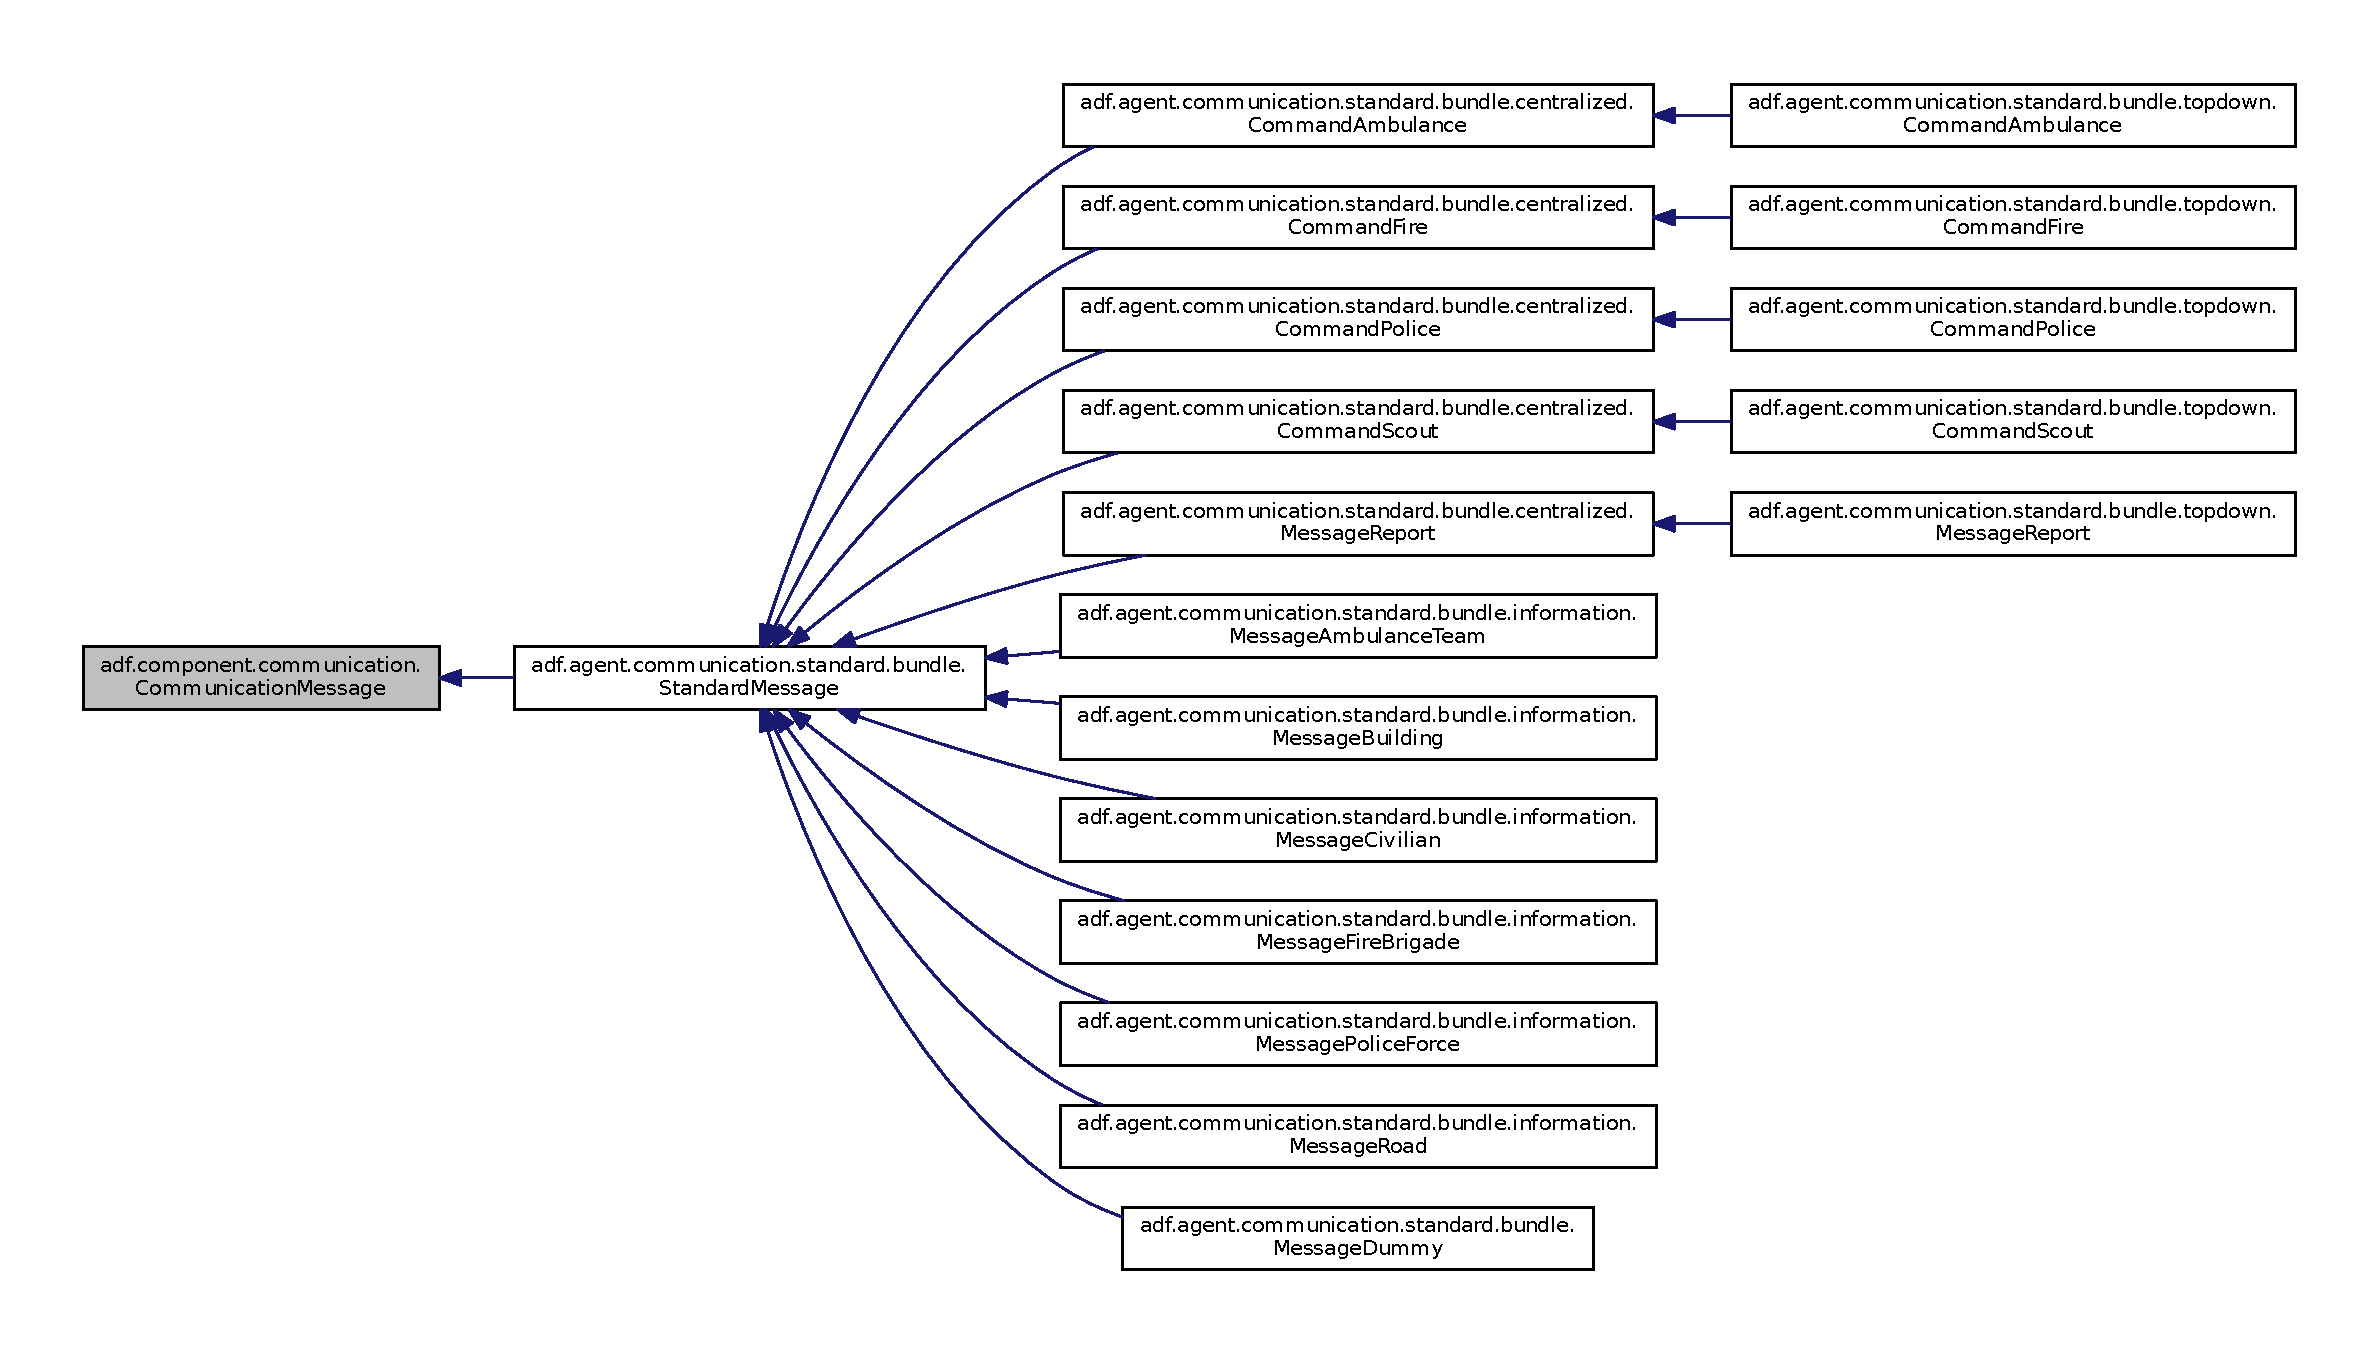
\includegraphics[width=350pt]{classadf_1_1component_1_1communication_1_1CommunicationMessage__inherit__graph}
\end{center}
\end{figure}
\subsection*{公開メンバ関数}
\begin{DoxyCompactItemize}
\item 
\hypertarget{classadf_1_1component_1_1communication_1_1CommunicationMessage_ac68a1589b60d7add1bde025ff02b64b3}{}\label{classadf_1_1component_1_1communication_1_1CommunicationMessage_ac68a1589b60d7add1bde025ff02b64b3} 
{\bfseries Communication\+Message} (boolean is\+Radio)
\item 
\hypertarget{classadf_1_1component_1_1communication_1_1CommunicationMessage_a353c19a8d7c6e052b1d50f580fe91cc6}{}\label{classadf_1_1component_1_1communication_1_1CommunicationMessage_a353c19a8d7c6e052b1d50f580fe91cc6} 
boolean {\bfseries is\+Radio} ()
\item 
\hypertarget{classadf_1_1component_1_1communication_1_1CommunicationMessage_a8d2694b5356bdd5126cc540b3f9f2f3a}{}\label{classadf_1_1component_1_1communication_1_1CommunicationMessage_a8d2694b5356bdd5126cc540b3f9f2f3a} 
abstract int {\bfseries get\+Byte\+Array\+Size} ()
\item 
\hypertarget{classadf_1_1component_1_1communication_1_1CommunicationMessage_a4b489e72be7259f0a61c1b85cce7f78b}{}\label{classadf_1_1component_1_1communication_1_1CommunicationMessage_a4b489e72be7259f0a61c1b85cce7f78b} 
abstract byte \mbox{[}$\,$\mbox{]} {\bfseries to\+Byte\+Array} ()
\item 
\hypertarget{classadf_1_1component_1_1communication_1_1CommunicationMessage_a35b04bf2a77eda6aba6070a02f4c26d3}{}\label{classadf_1_1component_1_1communication_1_1CommunicationMessage_a35b04bf2a77eda6aba6070a02f4c26d3} 
abstract \hyperlink{classadf_1_1component_1_1communication_1_1util_1_1BitOutputStream}{Bit\+Output\+Stream} {\bfseries to\+Bit\+Output\+Stream} ()
\item 
\hypertarget{classadf_1_1component_1_1communication_1_1CommunicationMessage_a64aef75735f3b938169ccc708a442dc0}{}\label{classadf_1_1component_1_1communication_1_1CommunicationMessage_a64aef75735f3b938169ccc708a442dc0} 
abstract String {\bfseries get\+Check\+Key} ()
\end{DoxyCompactItemize}


このクラス詳解は次のファイルから抽出されました\+:\begin{DoxyCompactItemize}
\item 
src/main/java/adf/component/communication/Communication\+Message.\+java\end{DoxyCompactItemize}

\hypertarget{classadf_1_1component_1_1communication_1_1CommunicationModule}{}\section{adf.\+component.\+communication.\+Communication\+Module Class Reference}
\label{classadf_1_1component_1_1communication_1_1CommunicationModule}\index{adf.\+component.\+communication.\+Communication\+Module@{adf.\+component.\+communication.\+Communication\+Module}}


Inheritance diagram for adf.\+component.\+communication.\+Communication\+Module\+:
\nopagebreak
\begin{figure}[H]
\begin{center}
\leavevmode
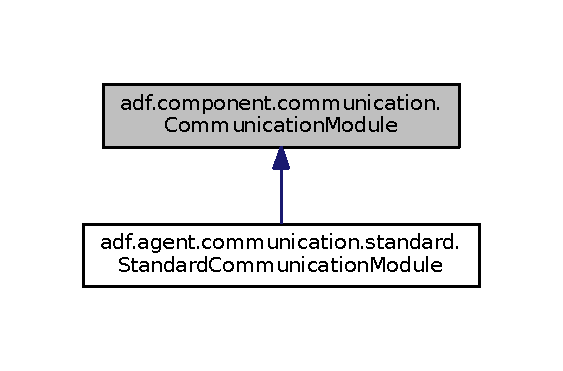
\includegraphics[width=270pt]{classadf_1_1component_1_1communication_1_1CommunicationModule__inherit__graph}
\end{center}
\end{figure}
\subsection*{Public Member Functions}
\begin{DoxyCompactItemize}
\item 
\hypertarget{classadf_1_1component_1_1communication_1_1CommunicationModule_a952c4d7e78483b49e4ad5b39f7a1c4c9}{}\label{classadf_1_1component_1_1communication_1_1CommunicationModule_a952c4d7e78483b49e4ad5b39f7a1c4c9} 
abstract void {\bfseries receive} (\hyperlink{classadf_1_1agent_1_1Agent}{Agent} agent, \hyperlink{classadf_1_1agent_1_1communication_1_1MessageManager}{Message\+Manager} message\+Manager)
\item 
\hypertarget{classadf_1_1component_1_1communication_1_1CommunicationModule_a1112befc9a69844215147728d08de734}{}\label{classadf_1_1component_1_1communication_1_1CommunicationModule_a1112befc9a69844215147728d08de734} 
abstract void {\bfseries send} (\hyperlink{classadf_1_1agent_1_1Agent}{Agent} agent, \hyperlink{classadf_1_1agent_1_1communication_1_1MessageManager}{Message\+Manager} message\+Manager)
\end{DoxyCompactItemize}


The documentation for this class was generated from the following file\+:\begin{DoxyCompactItemize}
\item 
src/main/java/adf/component/communication/Communication\+Module.\+java\end{DoxyCompactItemize}

\hypertarget{classadf_1_1launcher_1_1ConfigKey}{}\section{adf.\+launcher.\+Config\+Key Class Reference}
\label{classadf_1_1launcher_1_1ConfigKey}\index{adf.\+launcher.\+Config\+Key@{adf.\+launcher.\+Config\+Key}}
\subsection*{Static Public Attributes}
\begin{DoxyCompactItemize}
\item 
\hypertarget{classadf_1_1launcher_1_1ConfigKey_a8d68cfb5604916c75bb5c9ee358210d3}{}\label{classadf_1_1launcher_1_1ConfigKey_a8d68cfb5604916c75bb5c9ee358210d3} 
static final String {\bfseries K\+E\+Y\+\_\+\+L\+O\+A\+D\+E\+R\+\_\+\+C\+L\+A\+SS} = \char`\"{}adf.\+launcher.\+loader\char`\"{}
\item 
\hypertarget{classadf_1_1launcher_1_1ConfigKey_aeff8ee3a58dab2e14a806b1fe6ec2b46}{}\label{classadf_1_1launcher_1_1ConfigKey_aeff8ee3a58dab2e14a806b1fe6ec2b46} 
static final String {\bfseries K\+E\+Y\+\_\+\+P\+R\+E\+C\+O\+M\+P\+U\+TE} = \char`\"{}adf.\+launcher.\+precompute\char`\"{}
\item 
\hypertarget{classadf_1_1launcher_1_1ConfigKey_acce20feb471139f0348ad4866261b485}{}\label{classadf_1_1launcher_1_1ConfigKey_acce20feb471139f0348ad4866261b485} 
static final String {\bfseries K\+E\+Y\+\_\+\+M\+O\+D\+U\+L\+E\+\_\+\+C\+O\+N\+F\+I\+G\+\_\+\+F\+I\+L\+E\+\_\+\+N\+A\+ME} = \char`\"{}adf.\+agent.\+moduleconfig\char`\"{}
\item 
\hypertarget{classadf_1_1launcher_1_1ConfigKey_a448fe3a17e611cdb9d553fcb91c768ea}{}\label{classadf_1_1launcher_1_1ConfigKey_a448fe3a17e611cdb9d553fcb91c768ea} 
static final String {\bfseries K\+E\+Y\+\_\+\+D\+E\+B\+U\+G\+\_\+\+F\+L\+AG} = \char`\"{}adf.\+debug.\+flag\char`\"{}
\item 
\hypertarget{classadf_1_1launcher_1_1ConfigKey_a7a34844fe20b06d3ae3d7ee3717eccdb}{}\label{classadf_1_1launcher_1_1ConfigKey_a7a34844fe20b06d3ae3d7ee3717eccdb} 
static final String {\bfseries K\+E\+Y\+\_\+\+D\+E\+V\+E\+L\+O\+P\+\_\+\+F\+L\+AG} = \char`\"{}adf.\+develop.\+flag\char`\"{}
\item 
\hypertarget{classadf_1_1launcher_1_1ConfigKey_a766ab160d3b6cc5dfbbf194cc7964a81}{}\label{classadf_1_1launcher_1_1ConfigKey_a766ab160d3b6cc5dfbbf194cc7964a81} 
static final String {\bfseries K\+E\+Y\+\_\+\+D\+E\+V\+E\+L\+O\+P\+\_\+\+D\+A\+TA} = \char`\"{}adf.\+develop.\+data\char`\"{}
\item 
\hypertarget{classadf_1_1launcher_1_1ConfigKey_a6f15b699a23c72a180972aa94a87c1d0}{}\label{classadf_1_1launcher_1_1ConfigKey_a6f15b699a23c72a180972aa94a87c1d0} 
static final String {\bfseries K\+E\+Y\+\_\+\+D\+E\+V\+E\+L\+O\+P\+\_\+\+D\+A\+T\+A\+\_\+\+F\+I\+L\+E\+\_\+\+N\+A\+ME} = \char`\"{}adf.\+develop.\+filename\char`\"{}
\item 
\hypertarget{classadf_1_1launcher_1_1ConfigKey_a83c4e3c1785b5f15d18579123de26c5e}{}\label{classadf_1_1launcher_1_1ConfigKey_a83c4e3c1785b5f15d18579123de26c5e} 
static final String {\bfseries K\+E\+Y\+\_\+\+A\+M\+B\+U\+L\+A\+N\+C\+E\+\_\+\+T\+E\+A\+M\+\_\+\+C\+O\+U\+NT} = \char`\"{}adf.\+team.\+platoon.\+ambulance.\+count\char`\"{}
\item 
\hypertarget{classadf_1_1launcher_1_1ConfigKey_a753cf9e721aefb1eb0daffaaef78e08c}{}\label{classadf_1_1launcher_1_1ConfigKey_a753cf9e721aefb1eb0daffaaef78e08c} 
static final String {\bfseries K\+E\+Y\+\_\+\+F\+I\+R\+E\+\_\+\+B\+R\+I\+G\+A\+D\+E\+\_\+\+C\+O\+U\+NT} = \char`\"{}adf.\+team.\+platoon.\+fire.\+count\char`\"{}
\item 
\hypertarget{classadf_1_1launcher_1_1ConfigKey_af2da4cab9f474b02da3727a596b5aa92}{}\label{classadf_1_1launcher_1_1ConfigKey_af2da4cab9f474b02da3727a596b5aa92} 
static final String {\bfseries K\+E\+Y\+\_\+\+P\+O\+L\+I\+C\+E\+\_\+\+F\+O\+R\+C\+E\+\_\+\+C\+O\+U\+NT} = \char`\"{}adf.\+team.\+platoon.\+police.\+count\char`\"{}
\item 
\hypertarget{classadf_1_1launcher_1_1ConfigKey_a382f104371b41b3f1622f216d4a1eb96}{}\label{classadf_1_1launcher_1_1ConfigKey_a382f104371b41b3f1622f216d4a1eb96} 
static final String {\bfseries K\+E\+Y\+\_\+\+A\+M\+B\+U\+L\+A\+N\+C\+E\+\_\+\+C\+E\+N\+T\+R\+E\+\_\+\+C\+O\+U\+NT} = \char`\"{}adf.\+team.\+office.\+ambulance.\+count\char`\"{}
\item 
\hypertarget{classadf_1_1launcher_1_1ConfigKey_ac2cafe080c33a0235e7b1fd4208d11af}{}\label{classadf_1_1launcher_1_1ConfigKey_ac2cafe080c33a0235e7b1fd4208d11af} 
static final String {\bfseries K\+E\+Y\+\_\+\+F\+I\+R\+E\+\_\+\+S\+T\+A\+T\+I\+O\+N\+\_\+\+C\+O\+U\+NT} = \char`\"{}adf.\+team.\+office.\+fire.\+count\char`\"{}
\item 
\hypertarget{classadf_1_1launcher_1_1ConfigKey_ae89d1a0ee70adf2736e98539cab90b8d}{}\label{classadf_1_1launcher_1_1ConfigKey_ae89d1a0ee70adf2736e98539cab90b8d} 
static final String {\bfseries K\+E\+Y\+\_\+\+P\+O\+L\+I\+C\+E\+\_\+\+O\+F\+F\+I\+C\+E\+\_\+\+C\+O\+U\+NT} = \char`\"{}adf.\+team.\+office.\+police.\+count\char`\"{}
\end{DoxyCompactItemize}


The documentation for this class was generated from the following file\+:\begin{DoxyCompactItemize}
\item 
src/main/java/adf/launcher/Config\+Key.\+java\end{DoxyCompactItemize}

\hypertarget{classadf_1_1launcher_1_1connect_1_1Connector}{}\section{adf.\+launcher.\+connect.\+Connector クラス}
\label{classadf_1_1launcher_1_1connect_1_1Connector}\index{adf.\+launcher.\+connect.\+Connector@{adf.\+launcher.\+connect.\+Connector}}


adf.\+launcher.\+connect.\+Connector の継承関係図
\nopagebreak
\begin{figure}[H]
\begin{center}
\leavevmode
\includegraphics[width=350pt]{classadf_1_1launcher_1_1connect_1_1Connector__inherit__graph}
\end{center}
\end{figure}
\subsection*{公開メンバ関数}
\begin{DoxyCompactItemize}
\item 
\hypertarget{classadf_1_1launcher_1_1connect_1_1Connector_a0a0ac7fbfd9dd2849165907439b972e5}{}\label{classadf_1_1launcher_1_1connect_1_1Connector_a0a0ac7fbfd9dd2849165907439b972e5} 
abstract void {\bfseries connect} (Component\+Launcher launcher, Config config, \hyperlink{classadf_1_1component_1_1AbstractLoader}{Abstract\+Loader} loader)
\item 
\hypertarget{classadf_1_1launcher_1_1connect_1_1Connector_adb8014f72e8e70fe7eb877b17e7c9f7d}{}\label{classadf_1_1launcher_1_1connect_1_1Connector_adb8014f72e8e70fe7eb877b17e7c9f7d} 
int {\bfseries get\+Count\+Connected} ()
\end{DoxyCompactItemize}


このクラス詳解は次のファイルから抽出されました\+:\begin{DoxyCompactItemize}
\item 
src/main/java/adf/launcher/connect/Connector.\+java\end{DoxyCompactItemize}

\hypertarget{classadf_1_1launcher_1_1connect_1_1ConnectorAmbulanceCentre}{}\section{adf.\+launcher.\+connect.\+Connector\+Ambulance\+Centre Class Reference}
\label{classadf_1_1launcher_1_1connect_1_1ConnectorAmbulanceCentre}\index{adf.\+launcher.\+connect.\+Connector\+Ambulance\+Centre@{adf.\+launcher.\+connect.\+Connector\+Ambulance\+Centre}}


Inheritance diagram for adf.\+launcher.\+connect.\+Connector\+Ambulance\+Centre\+:
\nopagebreak
\begin{figure}[H]
\begin{center}
\leavevmode
\includegraphics[width=250pt]{classadf_1_1launcher_1_1connect_1_1ConnectorAmbulanceCentre__inherit__graph}
\end{center}
\end{figure}


Collaboration diagram for adf.\+launcher.\+connect.\+Connector\+Ambulance\+Centre\+:
\nopagebreak
\begin{figure}[H]
\begin{center}
\leavevmode
\includegraphics[width=250pt]{classadf_1_1launcher_1_1connect_1_1ConnectorAmbulanceCentre__coll__graph}
\end{center}
\end{figure}
\subsection*{Public Member Functions}
\begin{DoxyCompactItemize}
\item 
\hypertarget{classadf_1_1launcher_1_1connect_1_1ConnectorAmbulanceCentre_a82e17ab030924e8c0d2b53d030dc330e}{}\label{classadf_1_1launcher_1_1connect_1_1ConnectorAmbulanceCentre_a82e17ab030924e8c0d2b53d030dc330e} 
void {\bfseries connect} (Component\+Launcher launcher, Config config, \hyperlink{classadf_1_1component_1_1AbstractLoader}{Abstract\+Loader} loader)
\end{DoxyCompactItemize}


The documentation for this class was generated from the following file\+:\begin{DoxyCompactItemize}
\item 
src/main/java/adf/launcher/connect/Connector\+Ambulance\+Centre.\+java\end{DoxyCompactItemize}

\hypertarget{classadf_1_1launcher_1_1connect_1_1ConnectorAmbulanceTeam}{}\section{adf.\+launcher.\+connect.\+Connector\+Ambulance\+Team Class Reference}
\label{classadf_1_1launcher_1_1connect_1_1ConnectorAmbulanceTeam}\index{adf.\+launcher.\+connect.\+Connector\+Ambulance\+Team@{adf.\+launcher.\+connect.\+Connector\+Ambulance\+Team}}


Inheritance diagram for adf.\+launcher.\+connect.\+Connector\+Ambulance\+Team\+:
\nopagebreak
\begin{figure}[H]
\begin{center}
\leavevmode
\includegraphics[width=250pt]{classadf_1_1launcher_1_1connect_1_1ConnectorAmbulanceTeam__inherit__graph}
\end{center}
\end{figure}


Collaboration diagram for adf.\+launcher.\+connect.\+Connector\+Ambulance\+Team\+:
\nopagebreak
\begin{figure}[H]
\begin{center}
\leavevmode
\includegraphics[width=250pt]{classadf_1_1launcher_1_1connect_1_1ConnectorAmbulanceTeam__coll__graph}
\end{center}
\end{figure}
\subsection*{Public Member Functions}
\begin{DoxyCompactItemize}
\item 
\hypertarget{classadf_1_1launcher_1_1connect_1_1ConnectorAmbulanceTeam_ab8d91536ca43dc890644f58e8a8c45ef}{}\label{classadf_1_1launcher_1_1connect_1_1ConnectorAmbulanceTeam_ab8d91536ca43dc890644f58e8a8c45ef} 
void {\bfseries connect} (Component\+Launcher launcher, Config config, \hyperlink{classadf_1_1component_1_1AbstractLoader}{Abstract\+Loader} loader)
\end{DoxyCompactItemize}


The documentation for this class was generated from the following file\+:\begin{DoxyCompactItemize}
\item 
src/main/java/adf/launcher/connect/Connector\+Ambulance\+Team.\+java\end{DoxyCompactItemize}

\hypertarget{classadf_1_1launcher_1_1connect_1_1ConnectorFireBrigade}{}\section{adf.\+launcher.\+connect.\+Connector\+Fire\+Brigade クラス}
\label{classadf_1_1launcher_1_1connect_1_1ConnectorFireBrigade}\index{adf.\+launcher.\+connect.\+Connector\+Fire\+Brigade@{adf.\+launcher.\+connect.\+Connector\+Fire\+Brigade}}


adf.\+launcher.\+connect.\+Connector\+Fire\+Brigade の継承関係図
\nopagebreak
\begin{figure}[H]
\begin{center}
\leavevmode
\includegraphics[width=250pt]{classadf_1_1launcher_1_1connect_1_1ConnectorFireBrigade__inherit__graph}
\end{center}
\end{figure}


adf.\+launcher.\+connect.\+Connector\+Fire\+Brigade 連携図
\nopagebreak
\begin{figure}[H]
\begin{center}
\leavevmode
\includegraphics[width=250pt]{classadf_1_1launcher_1_1connect_1_1ConnectorFireBrigade__coll__graph}
\end{center}
\end{figure}
\subsection*{公開メンバ関数}
\begin{DoxyCompactItemize}
\item 
\hypertarget{classadf_1_1launcher_1_1connect_1_1ConnectorFireBrigade_ae430ca086d1713107280806dd69656cb}{}\label{classadf_1_1launcher_1_1connect_1_1ConnectorFireBrigade_ae430ca086d1713107280806dd69656cb} 
void {\bfseries connect} (Component\+Launcher launcher, Config config, \hyperlink{classadf_1_1component_1_1AbstractLoader}{Abstract\+Loader} loader)
\end{DoxyCompactItemize}


このクラス詳解は次のファイルから抽出されました\+:\begin{DoxyCompactItemize}
\item 
src/main/java/adf/launcher/connect/Connector\+Fire\+Brigade.\+java\end{DoxyCompactItemize}

\hypertarget{classadf_1_1launcher_1_1connect_1_1ConnectorFireStation}{}\section{adf.\+launcher.\+connect.\+Connector\+Fire\+Station クラス}
\label{classadf_1_1launcher_1_1connect_1_1ConnectorFireStation}\index{adf.\+launcher.\+connect.\+Connector\+Fire\+Station@{adf.\+launcher.\+connect.\+Connector\+Fire\+Station}}


adf.\+launcher.\+connect.\+Connector\+Fire\+Station の継承関係図
\nopagebreak
\begin{figure}[H]
\begin{center}
\leavevmode
\includegraphics[width=250pt]{classadf_1_1launcher_1_1connect_1_1ConnectorFireStation__inherit__graph}
\end{center}
\end{figure}


adf.\+launcher.\+connect.\+Connector\+Fire\+Station 連携図
\nopagebreak
\begin{figure}[H]
\begin{center}
\leavevmode
\includegraphics[width=250pt]{classadf_1_1launcher_1_1connect_1_1ConnectorFireStation__coll__graph}
\end{center}
\end{figure}
\subsection*{公開メンバ関数}
\begin{DoxyCompactItemize}
\item 
\hypertarget{classadf_1_1launcher_1_1connect_1_1ConnectorFireStation_add7763c53218ab2336b6a5f5873790aa}{}\label{classadf_1_1launcher_1_1connect_1_1ConnectorFireStation_add7763c53218ab2336b6a5f5873790aa} 
void {\bfseries connect} (Component\+Launcher launcher, Config config, \hyperlink{classadf_1_1component_1_1AbstractLoader}{Abstract\+Loader} loader)
\end{DoxyCompactItemize}


このクラス詳解は次のファイルから抽出されました\+:\begin{DoxyCompactItemize}
\item 
src/main/java/adf/launcher/connect/Connector\+Fire\+Station.\+java\end{DoxyCompactItemize}

\hypertarget{classadf_1_1launcher_1_1connect_1_1ConnectorPoliceForce}{}\section{adf.\+launcher.\+connect.\+Connector\+Police\+Force クラス}
\label{classadf_1_1launcher_1_1connect_1_1ConnectorPoliceForce}\index{adf.\+launcher.\+connect.\+Connector\+Police\+Force@{adf.\+launcher.\+connect.\+Connector\+Police\+Force}}


adf.\+launcher.\+connect.\+Connector\+Police\+Force の継承関係図
\nopagebreak
\begin{figure}[H]
\begin{center}
\leavevmode
\includegraphics[width=250pt]{classadf_1_1launcher_1_1connect_1_1ConnectorPoliceForce__inherit__graph}
\end{center}
\end{figure}


adf.\+launcher.\+connect.\+Connector\+Police\+Force 連携図
\nopagebreak
\begin{figure}[H]
\begin{center}
\leavevmode
\includegraphics[width=250pt]{classadf_1_1launcher_1_1connect_1_1ConnectorPoliceForce__coll__graph}
\end{center}
\end{figure}
\subsection*{公開メンバ関数}
\begin{DoxyCompactItemize}
\item 
\hypertarget{classadf_1_1launcher_1_1connect_1_1ConnectorPoliceForce_a21bcf528d065965b241cec3d77c0bed8}{}\label{classadf_1_1launcher_1_1connect_1_1ConnectorPoliceForce_a21bcf528d065965b241cec3d77c0bed8} 
void {\bfseries connect} (Component\+Launcher launcher, Config config, \hyperlink{classadf_1_1component_1_1AbstractLoader}{Abstract\+Loader} loader)
\end{DoxyCompactItemize}


このクラス詳解は次のファイルから抽出されました\+:\begin{DoxyCompactItemize}
\item 
src/main/java/adf/launcher/connect/Connector\+Police\+Force.\+java\end{DoxyCompactItemize}

\hypertarget{classadf_1_1launcher_1_1connect_1_1ConnectorPoliceOffice}{}\section{adf.\+launcher.\+connect.\+Connector\+Police\+Office クラス}
\label{classadf_1_1launcher_1_1connect_1_1ConnectorPoliceOffice}\index{adf.\+launcher.\+connect.\+Connector\+Police\+Office@{adf.\+launcher.\+connect.\+Connector\+Police\+Office}}


adf.\+launcher.\+connect.\+Connector\+Police\+Office の継承関係図
\nopagebreak
\begin{figure}[H]
\begin{center}
\leavevmode
\includegraphics[width=250pt]{classadf_1_1launcher_1_1connect_1_1ConnectorPoliceOffice__inherit__graph}
\end{center}
\end{figure}


adf.\+launcher.\+connect.\+Connector\+Police\+Office 連携図
\nopagebreak
\begin{figure}[H]
\begin{center}
\leavevmode
\includegraphics[width=250pt]{classadf_1_1launcher_1_1connect_1_1ConnectorPoliceOffice__coll__graph}
\end{center}
\end{figure}
\subsection*{公開メンバ関数}
\begin{DoxyCompactItemize}
\item 
\hypertarget{classadf_1_1launcher_1_1connect_1_1ConnectorPoliceOffice_a3f3c777ef185ec0b4e47678a2213310b}{}\label{classadf_1_1launcher_1_1connect_1_1ConnectorPoliceOffice_a3f3c777ef185ec0b4e47678a2213310b} 
void {\bfseries connect} (Component\+Launcher launcher, Config config, \hyperlink{classadf_1_1component_1_1AbstractLoader}{Abstract\+Loader} loader)
\end{DoxyCompactItemize}


このクラス詳解は次のファイルから抽出されました\+:\begin{DoxyCompactItemize}
\item 
src/main/java/adf/launcher/connect/Connector\+Police\+Office.\+java\end{DoxyCompactItemize}

\hypertarget{classadf_1_1launcher_1_1ConsoleOutput}{}\section{adf.\+launcher.\+Console\+Output クラス}
\label{classadf_1_1launcher_1_1ConsoleOutput}\index{adf.\+launcher.\+Console\+Output@{adf.\+launcher.\+Console\+Output}}
\subsection*{クラス}
\begin{DoxyCompactItemize}
\item 
enum {\bfseries State}
\end{DoxyCompactItemize}
\subsection*{静的公開メンバ関数}
\begin{DoxyCompactItemize}
\item 
\hypertarget{classadf_1_1launcher_1_1ConsoleOutput_a489dce085b6f89ac2b703fcd966cb721}{}\label{classadf_1_1launcher_1_1ConsoleOutput_a489dce085b6f89ac2b703fcd966cb721} 
static void {\bfseries out} (State state, String out)
\item 
\hypertarget{classadf_1_1launcher_1_1ConsoleOutput_af98d7716ff42556c2e05d9574a65800b}{}\label{classadf_1_1launcher_1_1ConsoleOutput_af98d7716ff42556c2e05d9574a65800b} 
static void {\bfseries info} (String out)
\item 
\hypertarget{classadf_1_1launcher_1_1ConsoleOutput_ab0e6c05ce0706c70b485609765727071}{}\label{classadf_1_1launcher_1_1ConsoleOutput_ab0e6c05ce0706c70b485609765727071} 
static void {\bfseries warn} (String out)
\item 
\hypertarget{classadf_1_1launcher_1_1ConsoleOutput_aedb5bbfe8ed04f70ed1a68336e9eb4eb}{}\label{classadf_1_1launcher_1_1ConsoleOutput_aedb5bbfe8ed04f70ed1a68336e9eb4eb} 
static void {\bfseries error} (String out)
\item 
\hypertarget{classadf_1_1launcher_1_1ConsoleOutput_ad780ff9a8c8301c2589a1e127b87364d}{}\label{classadf_1_1launcher_1_1ConsoleOutput_ad780ff9a8c8301c2589a1e127b87364d} 
static void {\bfseries notice} (String out)
\item 
\hypertarget{classadf_1_1launcher_1_1ConsoleOutput_a268f0b3d9513f834dc4be545cc74c6fd}{}\label{classadf_1_1launcher_1_1ConsoleOutput_a268f0b3d9513f834dc4be545cc74c6fd} 
static void {\bfseries start} (String out)
\item 
\hypertarget{classadf_1_1launcher_1_1ConsoleOutput_aa24a2f065c7f578465d966304f992f57}{}\label{classadf_1_1launcher_1_1ConsoleOutput_aa24a2f065c7f578465d966304f992f57} 
static void {\bfseries finish} (String out)
\item 
\hypertarget{classadf_1_1launcher_1_1ConsoleOutput_a8ea55b53f57fa18caba623dd841fbac6}{}\label{classadf_1_1launcher_1_1ConsoleOutput_a8ea55b53f57fa18caba623dd841fbac6} 
static void {\bfseries version} ()
\end{DoxyCompactItemize}


このクラス詳解は次のファイルから抽出されました\+:\begin{DoxyCompactItemize}
\item 
src/main/java/adf/launcher/Console\+Output.\+java\end{DoxyCompactItemize}

\hypertarget{classadf_1_1component_1_1control_1_1Control}{}\section{adf.\+component.\+control.\+Control Class Reference}
\label{classadf_1_1component_1_1control_1_1Control}\index{adf.\+component.\+control.\+Control@{adf.\+component.\+control.\+Control}}


Inheritance diagram for adf.\+component.\+control.\+Control\+:
\nopagebreak
\begin{figure}[H]
\begin{center}
\leavevmode
\includegraphics[width=244pt]{classadf_1_1component_1_1control_1_1Control__inherit__graph}
\end{center}
\end{figure}


Collaboration diagram for adf.\+component.\+control.\+Control\+:
\nopagebreak
\begin{figure}[H]
\begin{center}
\leavevmode
\includegraphics[width=244pt]{classadf_1_1component_1_1control_1_1Control__coll__graph}
\end{center}
\end{figure}
\subsection*{Public Member Functions}
\begin{DoxyCompactItemize}
\item 
\hypertarget{classadf_1_1component_1_1control_1_1Control_aeaab5064a2bfb271229b3b62a91c471c}{}\label{classadf_1_1component_1_1control_1_1Control_aeaab5064a2bfb271229b3b62a91c471c} 
{\bfseries Control} (\hyperlink{classadf_1_1component_1_1control_1_1Control}{Control} parent)
\item 
\hypertarget{classadf_1_1component_1_1control_1_1Control_a9107790ea778ff584c60b3939088d512}{}\label{classadf_1_1component_1_1control_1_1Control_a9107790ea778ff584c60b3939088d512} 
void {\bfseries initialize} (\hyperlink{classadf_1_1agent_1_1info_1_1AgentInfo}{Agent\+Info} agent\+Info, \hyperlink{classadf_1_1agent_1_1info_1_1WorldInfo}{World\+Info} world\+Info, \hyperlink{classadf_1_1agent_1_1info_1_1ScenarioInfo}{Scenario\+Info} scenario\+Info, \hyperlink{classadf_1_1agent_1_1module_1_1ModuleManager}{Module\+Manager} module\+Manager, \hyperlink{classadf_1_1agent_1_1communication_1_1MessageManager}{Message\+Manager} message\+Manager, \hyperlink{classadf_1_1agent_1_1develop_1_1DevelopData}{Develop\+Data} develop\+Data)
\item 
\hypertarget{classadf_1_1component_1_1control_1_1Control_ad9dfcd335a556fb0a3e3be9879a9656e}{}\label{classadf_1_1component_1_1control_1_1Control_ad9dfcd335a556fb0a3e3be9879a9656e} 
void {\bfseries resume} (\hyperlink{classadf_1_1agent_1_1info_1_1AgentInfo}{Agent\+Info} agent\+Info, \hyperlink{classadf_1_1agent_1_1info_1_1WorldInfo}{World\+Info} world\+Info, \hyperlink{classadf_1_1agent_1_1info_1_1ScenarioInfo}{Scenario\+Info} scenario\+Info, \hyperlink{classadf_1_1agent_1_1module_1_1ModuleManager}{Module\+Manager} module\+Manager, \hyperlink{classadf_1_1agent_1_1precompute_1_1PrecomputeData}{Precompute\+Data} precompute\+Info, \hyperlink{classadf_1_1agent_1_1develop_1_1DevelopData}{Develop\+Data} develop\+Data)
\item 
\hypertarget{classadf_1_1component_1_1control_1_1Control_a5cb4d26b41cd93b2a0ea06963c71fee5}{}\label{classadf_1_1component_1_1control_1_1Control_a5cb4d26b41cd93b2a0ea06963c71fee5} 
void {\bfseries preparate} (\hyperlink{classadf_1_1agent_1_1info_1_1AgentInfo}{Agent\+Info} agent\+Info, \hyperlink{classadf_1_1agent_1_1info_1_1WorldInfo}{World\+Info} world\+Info, \hyperlink{classadf_1_1agent_1_1info_1_1ScenarioInfo}{Scenario\+Info} scenario\+Info, \hyperlink{classadf_1_1agent_1_1module_1_1ModuleManager}{Module\+Manager} module\+Manager, \hyperlink{classadf_1_1agent_1_1develop_1_1DevelopData}{Develop\+Data} develop\+Data)
\item 
\hypertarget{classadf_1_1component_1_1control_1_1Control_ad8d7e05c1d5e6ac44e50c79a3ab14706}{}\label{classadf_1_1component_1_1control_1_1Control_ad8d7e05c1d5e6ac44e50c79a3ab14706} 
void {\bfseries think} (\hyperlink{classadf_1_1agent_1_1info_1_1AgentInfo}{Agent\+Info} agent\+Info, \hyperlink{classadf_1_1agent_1_1info_1_1WorldInfo}{World\+Info} world\+Info, \hyperlink{classadf_1_1agent_1_1info_1_1ScenarioInfo}{Scenario\+Info} scenario\+Info, \hyperlink{classadf_1_1agent_1_1module_1_1ModuleManager}{Module\+Manager} module\+Manager, \hyperlink{classadf_1_1agent_1_1communication_1_1MessageManager}{Message\+Manager} message\+Manager, \hyperlink{classadf_1_1agent_1_1develop_1_1DevelopData}{Develop\+Data} develop\+Data)
\item 
\hypertarget{classadf_1_1component_1_1control_1_1Control_adccbe65c8b9e73ebb17d8dd53273f41d}{}\label{classadf_1_1component_1_1control_1_1Control_adccbe65c8b9e73ebb17d8dd53273f41d} 
\hyperlink{classadf_1_1component_1_1control_1_1Control}{Control} {\bfseries get\+Parent\+Control} ()
\end{DoxyCompactItemize}


\subsection{Detailed Description}
\begin{DoxyRefDesc}{Deprecated}
\item[\hyperlink{deprecated__deprecated000009}{Deprecated}]change class name \hyperlink{}{Tactics\+Center} \end{DoxyRefDesc}


The documentation for this class was generated from the following file\+:\begin{DoxyCompactItemize}
\item 
src/main/java/adf/component/control/Control.\+java\end{DoxyCompactItemize}

\hypertarget{classadf_1_1component_1_1control_1_1ControlAmbulance}{}\section{adf.\+component.\+control.\+Control\+Ambulance Class Reference}
\label{classadf_1_1component_1_1control_1_1ControlAmbulance}\index{adf.\+component.\+control.\+Control\+Ambulance@{adf.\+component.\+control.\+Control\+Ambulance}}


Inheritance diagram for adf.\+component.\+control.\+Control\+Ambulance\+:
\nopagebreak
\begin{figure}[H]
\begin{center}
\leavevmode
\includegraphics[width=244pt]{classadf_1_1component_1_1control_1_1ControlAmbulance__inherit__graph}
\end{center}
\end{figure}


Collaboration diagram for adf.\+component.\+control.\+Control\+Ambulance\+:
\nopagebreak
\begin{figure}[H]
\begin{center}
\leavevmode
\includegraphics[width=244pt]{classadf_1_1component_1_1control_1_1ControlAmbulance__coll__graph}
\end{center}
\end{figure}
\subsection*{Public Member Functions}
\begin{DoxyCompactItemize}
\item 
\hypertarget{classadf_1_1component_1_1control_1_1ControlAmbulance_ade5e6a6110e83443fbef51dec9d2723b}{}\label{classadf_1_1component_1_1control_1_1ControlAmbulance_ade5e6a6110e83443fbef51dec9d2723b} 
{\bfseries Control\+Ambulance} (\hyperlink{classadf_1_1component_1_1control_1_1ControlAmbulance}{Control\+Ambulance} parent)
\end{DoxyCompactItemize}


The documentation for this class was generated from the following file\+:\begin{DoxyCompactItemize}
\item 
src/main/java/adf/component/control/Control\+Ambulance.\+java\end{DoxyCompactItemize}

\hypertarget{classadf_1_1component_1_1control_1_1ControlFire}{}\section{adf.\+component.\+control.\+Control\+Fire Class Reference}
\label{classadf_1_1component_1_1control_1_1ControlFire}\index{adf.\+component.\+control.\+Control\+Fire@{adf.\+component.\+control.\+Control\+Fire}}


Inheritance diagram for adf.\+component.\+control.\+Control\+Fire\+:
\nopagebreak
\begin{figure}[H]
\begin{center}
\leavevmode
\includegraphics[width=262pt]{classadf_1_1component_1_1control_1_1ControlFire__inherit__graph}
\end{center}
\end{figure}


Collaboration diagram for adf.\+component.\+control.\+Control\+Fire\+:
\nopagebreak
\begin{figure}[H]
\begin{center}
\leavevmode
\includegraphics[width=262pt]{classadf_1_1component_1_1control_1_1ControlFire__coll__graph}
\end{center}
\end{figure}
\subsection*{Public Member Functions}
\begin{DoxyCompactItemize}
\item 
\hypertarget{classadf_1_1component_1_1control_1_1ControlFire_a868120301fcf4b970ef05401798baca6}{}\label{classadf_1_1component_1_1control_1_1ControlFire_a868120301fcf4b970ef05401798baca6} 
{\bfseries Control\+Fire} (\hyperlink{classadf_1_1component_1_1control_1_1ControlFire}{Control\+Fire} parent)
\end{DoxyCompactItemize}


The documentation for this class was generated from the following file\+:\begin{DoxyCompactItemize}
\item 
src/main/java/adf/component/control/Control\+Fire.\+java\end{DoxyCompactItemize}

\hypertarget{classadf_1_1component_1_1control_1_1ControlPolice}{}\section{adf.\+component.\+control.\+Control\+Police Class Reference}
\label{classadf_1_1component_1_1control_1_1ControlPolice}\index{adf.\+component.\+control.\+Control\+Police@{adf.\+component.\+control.\+Control\+Police}}


Inheritance diagram for adf.\+component.\+control.\+Control\+Police\+:
\nopagebreak
\begin{figure}[H]
\begin{center}
\leavevmode
\includegraphics[width=244pt]{classadf_1_1component_1_1control_1_1ControlPolice__inherit__graph}
\end{center}
\end{figure}


Collaboration diagram for adf.\+component.\+control.\+Control\+Police\+:
\nopagebreak
\begin{figure}[H]
\begin{center}
\leavevmode
\includegraphics[width=244pt]{classadf_1_1component_1_1control_1_1ControlPolice__coll__graph}
\end{center}
\end{figure}
\subsection*{Public Member Functions}
\begin{DoxyCompactItemize}
\item 
\hypertarget{classadf_1_1component_1_1control_1_1ControlPolice_a5f749280b92a7b6785bf6207f91834f8}{}\label{classadf_1_1component_1_1control_1_1ControlPolice_a5f749280b92a7b6785bf6207f91834f8} 
{\bfseries Control\+Police} (\hyperlink{classadf_1_1component_1_1control_1_1ControlPolice}{Control\+Police} parent)
\end{DoxyCompactItemize}


The documentation for this class was generated from the following file\+:\begin{DoxyCompactItemize}
\item 
src/main/java/adf/component/control/Control\+Police.\+java\end{DoxyCompactItemize}

\hypertarget{classadf_1_1agent_1_1develop_1_1DevelopData}{}\section{adf.\+agent.\+develop.\+Develop\+Data クラス}
\label{classadf_1_1agent_1_1develop_1_1DevelopData}\index{adf.\+agent.\+develop.\+Develop\+Data@{adf.\+agent.\+develop.\+Develop\+Data}}
\subsection*{公開メンバ関数}
\begin{DoxyCompactItemize}
\item 
\hypertarget{classadf_1_1agent_1_1develop_1_1DevelopData_aef4cf489592feb7ff0a5947dbf7329cc}{}\label{classadf_1_1agent_1_1develop_1_1DevelopData_aef4cf489592feb7ff0a5947dbf7329cc} 
{\bfseries Develop\+Data} (boolean develop\+Flag, String develop\+Data\+File\+Name, List$<$ String $>$ raw\+Data)
\item 
\hypertarget{classadf_1_1agent_1_1develop_1_1DevelopData_aa504c579f983433f4b83b911e5808f2b}{}\label{classadf_1_1agent_1_1develop_1_1DevelopData_aa504c579f983433f4b83b911e5808f2b} 
boolean {\bfseries is\+Develop\+Mode} ()
\item 
\hypertarget{classadf_1_1agent_1_1develop_1_1DevelopData_af55569be14e228d98738d15d0214d0ad}{}\label{classadf_1_1agent_1_1develop_1_1DevelopData_af55569be14e228d98738d15d0214d0ad} 
Integer {\bfseries get\+Integer} (String name, int default\+Value)
\item 
\hypertarget{classadf_1_1agent_1_1develop_1_1DevelopData_a185a4a55199c5199943e6e18bc173d07}{}\label{classadf_1_1agent_1_1develop_1_1DevelopData_a185a4a55199c5199943e6e18bc173d07} 
Double {\bfseries get\+Double} (String name, double default\+Value)
\item 
\hypertarget{classadf_1_1agent_1_1develop_1_1DevelopData_a543879df41f6ac2c40406271d6f724ab}{}\label{classadf_1_1agent_1_1develop_1_1DevelopData_a543879df41f6ac2c40406271d6f724ab} 
Boolean {\bfseries get\+Boolean} (String name, boolean default\+Value)
\item 
\hypertarget{classadf_1_1agent_1_1develop_1_1DevelopData_a7cedf349b54c1337d6ae36eea73f3753}{}\label{classadf_1_1agent_1_1develop_1_1DevelopData_a7cedf349b54c1337d6ae36eea73f3753} 
String {\bfseries get\+String} (String name, String default\+Value)
\item 
\hypertarget{classadf_1_1agent_1_1develop_1_1DevelopData_a8b53099cdeed50c7a27c741851e1e459}{}\label{classadf_1_1agent_1_1develop_1_1DevelopData_a8b53099cdeed50c7a27c741851e1e459} 
List$<$ Integer $>$ {\bfseries get\+Integer\+List} (String name, List$<$ Integer $>$ default\+Value)
\item 
\hypertarget{classadf_1_1agent_1_1develop_1_1DevelopData_a20772951f2c49bbae32b285c23662221}{}\label{classadf_1_1agent_1_1develop_1_1DevelopData_a20772951f2c49bbae32b285c23662221} 
List$<$ Double $>$ {\bfseries get\+Double\+List} (String name, List$<$ Double $>$ default\+Value)
\item 
\hypertarget{classadf_1_1agent_1_1develop_1_1DevelopData_a94e976b28a65fbf8055e6283a31236cc}{}\label{classadf_1_1agent_1_1develop_1_1DevelopData_a94e976b28a65fbf8055e6283a31236cc} 
List$<$ Boolean $>$ {\bfseries get\+Boolean\+List} (String name, List$<$ Boolean $>$ default\+Value)
\item 
\hypertarget{classadf_1_1agent_1_1develop_1_1DevelopData_a5dd5fb6da9a779b77029a0135ce196aa}{}\label{classadf_1_1agent_1_1develop_1_1DevelopData_a5dd5fb6da9a779b77029a0135ce196aa} 
List$<$ String $>$ {\bfseries get\+String\+List} (String name, List$<$ String $>$ default\+Value)
\item 
\hypertarget{classadf_1_1agent_1_1develop_1_1DevelopData_a85d6ec19049355a23283aac6b93b4584}{}\label{classadf_1_1agent_1_1develop_1_1DevelopData_a85d6ec19049355a23283aac6b93b4584} 
void {\bfseries clear} ()
\end{DoxyCompactItemize}
\subsection*{静的公開変数類}
\begin{DoxyCompactItemize}
\item 
\hypertarget{classadf_1_1agent_1_1develop_1_1DevelopData_a854803523cdad900342fa22a3ba8efbb}{}\label{classadf_1_1agent_1_1develop_1_1DevelopData_a854803523cdad900342fa22a3ba8efbb} 
static final String {\bfseries D\+E\+F\+A\+U\+L\+T\+\_\+\+F\+I\+L\+E\+\_\+\+N\+A\+ME} = System.\+get\+Property(\char`\"{}user.\+dir\char`\"{}) + \char`\"{}data\char`\"{} + File.\+separator + \char`\"{}develop.\+json\char`\"{}
\end{DoxyCompactItemize}


このクラス詳解は次のファイルから抽出されました\+:\begin{DoxyCompactItemize}
\item 
src/main/java/adf/agent/develop/Develop\+Data.\+java\end{DoxyCompactItemize}

\hypertarget{classadf_1_1launcher_1_1dummy_1_1tactics_1_1DummyTacticsAmbulance}{}\section{adf.\+launcher.\+dummy.\+tactics.\+Dummy\+Tactics\+Ambulance Class Reference}
\label{classadf_1_1launcher_1_1dummy_1_1tactics_1_1DummyTacticsAmbulance}\index{adf.\+launcher.\+dummy.\+tactics.\+Dummy\+Tactics\+Ambulance@{adf.\+launcher.\+dummy.\+tactics.\+Dummy\+Tactics\+Ambulance}}


Inheritance diagram for adf.\+launcher.\+dummy.\+tactics.\+Dummy\+Tactics\+Ambulance\+:
\nopagebreak
\begin{figure}[H]
\begin{center}
\leavevmode
\includegraphics[width=241pt]{classadf_1_1launcher_1_1dummy_1_1tactics_1_1DummyTacticsAmbulance__inherit__graph}
\end{center}
\end{figure}


Collaboration diagram for adf.\+launcher.\+dummy.\+tactics.\+Dummy\+Tactics\+Ambulance\+:
\nopagebreak
\begin{figure}[H]
\begin{center}
\leavevmode
\includegraphics[width=241pt]{classadf_1_1launcher_1_1dummy_1_1tactics_1_1DummyTacticsAmbulance__coll__graph}
\end{center}
\end{figure}
\subsection*{Public Member Functions}
\begin{DoxyCompactItemize}
\item 
\hypertarget{classadf_1_1launcher_1_1dummy_1_1tactics_1_1DummyTacticsAmbulance_aa1592381d7fdb5a81a35eadd0a568b67}{}\label{classadf_1_1launcher_1_1dummy_1_1tactics_1_1DummyTacticsAmbulance_aa1592381d7fdb5a81a35eadd0a568b67} 
void {\bfseries initialize} (\hyperlink{classadf_1_1agent_1_1info_1_1AgentInfo}{Agent\+Info} agent\+Info, \hyperlink{classadf_1_1agent_1_1info_1_1WorldInfo}{World\+Info} world\+Info, \hyperlink{classadf_1_1agent_1_1info_1_1ScenarioInfo}{Scenario\+Info} scenario\+Info, \hyperlink{classadf_1_1agent_1_1module_1_1ModuleManager}{Module\+Manager} module\+Manager, \hyperlink{classadf_1_1agent_1_1communication_1_1MessageManager}{Message\+Manager} message\+Manager, \hyperlink{classadf_1_1agent_1_1develop_1_1DevelopData}{Develop\+Data} develop\+Data)
\item 
\hypertarget{classadf_1_1launcher_1_1dummy_1_1tactics_1_1DummyTacticsAmbulance_af5e46d66c7fa3d937170dc9803f7b9fa}{}\label{classadf_1_1launcher_1_1dummy_1_1tactics_1_1DummyTacticsAmbulance_af5e46d66c7fa3d937170dc9803f7b9fa} 
void {\bfseries precompute} (\hyperlink{classadf_1_1agent_1_1info_1_1AgentInfo}{Agent\+Info} agent\+Info, \hyperlink{classadf_1_1agent_1_1info_1_1WorldInfo}{World\+Info} world\+Info, \hyperlink{classadf_1_1agent_1_1info_1_1ScenarioInfo}{Scenario\+Info} scenario\+Info, \hyperlink{classadf_1_1agent_1_1module_1_1ModuleManager}{Module\+Manager} module\+Manager, \hyperlink{classadf_1_1agent_1_1precompute_1_1PrecomputeData}{Precompute\+Data} precompute\+Data, \hyperlink{classadf_1_1agent_1_1develop_1_1DevelopData}{Develop\+Data} develop\+Data)
\item 
\hypertarget{classadf_1_1launcher_1_1dummy_1_1tactics_1_1DummyTacticsAmbulance_a716e8aafc2ccdc9572d445a14bbf4aa5}{}\label{classadf_1_1launcher_1_1dummy_1_1tactics_1_1DummyTacticsAmbulance_a716e8aafc2ccdc9572d445a14bbf4aa5} 
void {\bfseries resume} (\hyperlink{classadf_1_1agent_1_1info_1_1AgentInfo}{Agent\+Info} agent\+Info, \hyperlink{classadf_1_1agent_1_1info_1_1WorldInfo}{World\+Info} world\+Info, \hyperlink{classadf_1_1agent_1_1info_1_1ScenarioInfo}{Scenario\+Info} scenario\+Info, \hyperlink{classadf_1_1agent_1_1module_1_1ModuleManager}{Module\+Manager} module\+Manager, \hyperlink{classadf_1_1agent_1_1precompute_1_1PrecomputeData}{Precompute\+Data} precompute\+Data, \hyperlink{classadf_1_1agent_1_1develop_1_1DevelopData}{Develop\+Data} develop\+Data)
\item 
\hypertarget{classadf_1_1launcher_1_1dummy_1_1tactics_1_1DummyTacticsAmbulance_afe5d0ed08352dbd161fcfcf065e39417}{}\label{classadf_1_1launcher_1_1dummy_1_1tactics_1_1DummyTacticsAmbulance_afe5d0ed08352dbd161fcfcf065e39417} 
void {\bfseries preparate} (\hyperlink{classadf_1_1agent_1_1info_1_1AgentInfo}{Agent\+Info} agent\+Info, \hyperlink{classadf_1_1agent_1_1info_1_1WorldInfo}{World\+Info} world\+Info, \hyperlink{classadf_1_1agent_1_1info_1_1ScenarioInfo}{Scenario\+Info} scenario\+Info, \hyperlink{classadf_1_1agent_1_1module_1_1ModuleManager}{Module\+Manager} module\+Manager, \hyperlink{classadf_1_1agent_1_1develop_1_1DevelopData}{Develop\+Data} develop\+Data)
\item 
\hypertarget{classadf_1_1launcher_1_1dummy_1_1tactics_1_1DummyTacticsAmbulance_a64caa7e1fee6348485753c247427777a}{}\label{classadf_1_1launcher_1_1dummy_1_1tactics_1_1DummyTacticsAmbulance_a64caa7e1fee6348485753c247427777a} 
\hyperlink{classadf_1_1agent_1_1action_1_1Action}{Action} {\bfseries think} (\hyperlink{classadf_1_1agent_1_1info_1_1AgentInfo}{Agent\+Info} agent\+Info, \hyperlink{classadf_1_1agent_1_1info_1_1WorldInfo}{World\+Info} world\+Info, \hyperlink{classadf_1_1agent_1_1info_1_1ScenarioInfo}{Scenario\+Info} scenario\+Info, \hyperlink{classadf_1_1agent_1_1module_1_1ModuleManager}{Module\+Manager} module\+Manager, \hyperlink{classadf_1_1agent_1_1communication_1_1MessageManager}{Message\+Manager} message\+Manager, \hyperlink{classadf_1_1agent_1_1develop_1_1DevelopData}{Develop\+Data} develop\+Data)
\end{DoxyCompactItemize}


The documentation for this class was generated from the following file\+:\begin{DoxyCompactItemize}
\item 
src/main/java/adf/launcher/dummy/tactics/Dummy\+Tactics\+Ambulance.\+java\end{DoxyCompactItemize}

\hypertarget{classadf_1_1launcher_1_1dummy_1_1control_1_1DummyTacticsAmbulanceCenter}{}\section{adf.\+launcher.\+dummy.\+control.\+Dummy\+Tactics\+Ambulance\+Center クラス}
\label{classadf_1_1launcher_1_1dummy_1_1control_1_1DummyTacticsAmbulanceCenter}\index{adf.\+launcher.\+dummy.\+control.\+Dummy\+Tactics\+Ambulance\+Center@{adf.\+launcher.\+dummy.\+control.\+Dummy\+Tactics\+Ambulance\+Center}}


adf.\+launcher.\+dummy.\+control.\+Dummy\+Tactics\+Ambulance\+Center の継承関係図
\nopagebreak
\begin{figure}[H]
\begin{center}
\leavevmode
\includegraphics[width=256pt]{classadf_1_1launcher_1_1dummy_1_1control_1_1DummyTacticsAmbulanceCenter__inherit__graph}
\end{center}
\end{figure}


adf.\+launcher.\+dummy.\+control.\+Dummy\+Tactics\+Ambulance\+Center 連携図
\nopagebreak
\begin{figure}[H]
\begin{center}
\leavevmode
\includegraphics[width=256pt]{classadf_1_1launcher_1_1dummy_1_1control_1_1DummyTacticsAmbulanceCenter__coll__graph}
\end{center}
\end{figure}
\subsection*{公開メンバ関数}
\begin{DoxyCompactItemize}
\item 
\hypertarget{classadf_1_1launcher_1_1dummy_1_1control_1_1DummyTacticsAmbulanceCenter_a2741eacb252085b755cb9ddf770dc230}{}\label{classadf_1_1launcher_1_1dummy_1_1control_1_1DummyTacticsAmbulanceCenter_a2741eacb252085b755cb9ddf770dc230} 
void {\bfseries initialize} (\hyperlink{classadf_1_1agent_1_1info_1_1AgentInfo}{Agent\+Info} agent\+Info, \hyperlink{classadf_1_1agent_1_1info_1_1WorldInfo}{World\+Info} world\+Info, \hyperlink{classadf_1_1agent_1_1info_1_1ScenarioInfo}{Scenario\+Info} scenario\+Info, \hyperlink{classadf_1_1agent_1_1module_1_1ModuleManager}{Module\+Manager} module\+Manager, \hyperlink{classadf_1_1agent_1_1communication_1_1MessageManager}{Message\+Manager} message\+Manager, \hyperlink{classadf_1_1agent_1_1develop_1_1DevelopData}{Develop\+Data} develop\+Data)
\item 
\hypertarget{classadf_1_1launcher_1_1dummy_1_1control_1_1DummyTacticsAmbulanceCenter_a59ed9eeb1c5d8b37bb3f3df6b2a8159f}{}\label{classadf_1_1launcher_1_1dummy_1_1control_1_1DummyTacticsAmbulanceCenter_a59ed9eeb1c5d8b37bb3f3df6b2a8159f} 
void {\bfseries resume} (\hyperlink{classadf_1_1agent_1_1info_1_1AgentInfo}{Agent\+Info} agent\+Info, \hyperlink{classadf_1_1agent_1_1info_1_1WorldInfo}{World\+Info} world\+Info, \hyperlink{classadf_1_1agent_1_1info_1_1ScenarioInfo}{Scenario\+Info} scenario\+Info, \hyperlink{classadf_1_1agent_1_1module_1_1ModuleManager}{Module\+Manager} module\+Manager, \hyperlink{classadf_1_1agent_1_1precompute_1_1PrecomputeData}{Precompute\+Data} precompute\+Info, \hyperlink{classadf_1_1agent_1_1develop_1_1DevelopData}{Develop\+Data} develop\+Data)
\item 
\hypertarget{classadf_1_1launcher_1_1dummy_1_1control_1_1DummyTacticsAmbulanceCenter_a9dfac45a4507e661809c2eeb10750d73}{}\label{classadf_1_1launcher_1_1dummy_1_1control_1_1DummyTacticsAmbulanceCenter_a9dfac45a4507e661809c2eeb10750d73} 
void {\bfseries preparate} (\hyperlink{classadf_1_1agent_1_1info_1_1AgentInfo}{Agent\+Info} agent\+Info, \hyperlink{classadf_1_1agent_1_1info_1_1WorldInfo}{World\+Info} world\+Info, \hyperlink{classadf_1_1agent_1_1info_1_1ScenarioInfo}{Scenario\+Info} scenario\+Info, \hyperlink{classadf_1_1agent_1_1module_1_1ModuleManager}{Module\+Manager} module\+Manager, \hyperlink{classadf_1_1agent_1_1develop_1_1DevelopData}{Develop\+Data} develop\+Data)
\item 
\hypertarget{classadf_1_1launcher_1_1dummy_1_1control_1_1DummyTacticsAmbulanceCenter_af6dbefc0ad86950c245ce54bb415c435}{}\label{classadf_1_1launcher_1_1dummy_1_1control_1_1DummyTacticsAmbulanceCenter_af6dbefc0ad86950c245ce54bb415c435} 
void {\bfseries think} (\hyperlink{classadf_1_1agent_1_1info_1_1AgentInfo}{Agent\+Info} agent\+Info, \hyperlink{classadf_1_1agent_1_1info_1_1WorldInfo}{World\+Info} world\+Info, \hyperlink{classadf_1_1agent_1_1info_1_1ScenarioInfo}{Scenario\+Info} scenario\+Info, \hyperlink{classadf_1_1agent_1_1module_1_1ModuleManager}{Module\+Manager} module\+Manager, \hyperlink{classadf_1_1agent_1_1communication_1_1MessageManager}{Message\+Manager} message\+Manager, \hyperlink{classadf_1_1agent_1_1develop_1_1DevelopData}{Develop\+Data} develop\+Data)
\end{DoxyCompactItemize}


このクラス詳解は次のファイルから抽出されました\+:\begin{DoxyCompactItemize}
\item 
src/main/java/adf/launcher/dummy/control/Dummy\+Tactics\+Ambulance\+Center.\+java\end{DoxyCompactItemize}

\hypertarget{classadf_1_1launcher_1_1dummy_1_1tactics_1_1DummyTacticsFire}{}\section{adf.\+launcher.\+dummy.\+tactics.\+Dummy\+Tactics\+Fire Class Reference}
\label{classadf_1_1launcher_1_1dummy_1_1tactics_1_1DummyTacticsFire}\index{adf.\+launcher.\+dummy.\+tactics.\+Dummy\+Tactics\+Fire@{adf.\+launcher.\+dummy.\+tactics.\+Dummy\+Tactics\+Fire}}


Inheritance diagram for adf.\+launcher.\+dummy.\+tactics.\+Dummy\+Tactics\+Fire\+:
\nopagebreak
\begin{figure}[H]
\begin{center}
\leavevmode
\includegraphics[width=258pt]{classadf_1_1launcher_1_1dummy_1_1tactics_1_1DummyTacticsFire__inherit__graph}
\end{center}
\end{figure}


Collaboration diagram for adf.\+launcher.\+dummy.\+tactics.\+Dummy\+Tactics\+Fire\+:
\nopagebreak
\begin{figure}[H]
\begin{center}
\leavevmode
\includegraphics[width=258pt]{classadf_1_1launcher_1_1dummy_1_1tactics_1_1DummyTacticsFire__coll__graph}
\end{center}
\end{figure}
\subsection*{Public Member Functions}
\begin{DoxyCompactItemize}
\item 
\hypertarget{classadf_1_1launcher_1_1dummy_1_1tactics_1_1DummyTacticsFire_a310015ec3bd973c1c0b204c2d0728688}{}\label{classadf_1_1launcher_1_1dummy_1_1tactics_1_1DummyTacticsFire_a310015ec3bd973c1c0b204c2d0728688} 
void {\bfseries initialize} (\hyperlink{classadf_1_1agent_1_1info_1_1AgentInfo}{Agent\+Info} agent\+Info, \hyperlink{classadf_1_1agent_1_1info_1_1WorldInfo}{World\+Info} world\+Info, \hyperlink{classadf_1_1agent_1_1info_1_1ScenarioInfo}{Scenario\+Info} scenario\+Info, \hyperlink{classadf_1_1agent_1_1module_1_1ModuleManager}{Module\+Manager} module\+Manager, \hyperlink{classadf_1_1agent_1_1communication_1_1MessageManager}{Message\+Manager} message\+Manager, \hyperlink{classadf_1_1agent_1_1develop_1_1DevelopData}{Develop\+Data} develop\+Data)
\item 
\hypertarget{classadf_1_1launcher_1_1dummy_1_1tactics_1_1DummyTacticsFire_aff4e403259b3ec9aeb3c68f4839e3d31}{}\label{classadf_1_1launcher_1_1dummy_1_1tactics_1_1DummyTacticsFire_aff4e403259b3ec9aeb3c68f4839e3d31} 
void {\bfseries precompute} (\hyperlink{classadf_1_1agent_1_1info_1_1AgentInfo}{Agent\+Info} agent\+Info, \hyperlink{classadf_1_1agent_1_1info_1_1WorldInfo}{World\+Info} world\+Info, \hyperlink{classadf_1_1agent_1_1info_1_1ScenarioInfo}{Scenario\+Info} scenario\+Info, \hyperlink{classadf_1_1agent_1_1module_1_1ModuleManager}{Module\+Manager} module\+Manager, \hyperlink{classadf_1_1agent_1_1precompute_1_1PrecomputeData}{Precompute\+Data} precompute\+Data, \hyperlink{classadf_1_1agent_1_1develop_1_1DevelopData}{Develop\+Data} develop\+Data)
\item 
\hypertarget{classadf_1_1launcher_1_1dummy_1_1tactics_1_1DummyTacticsFire_a29d6760bc439d944fca7fa4a0ec9f69d}{}\label{classadf_1_1launcher_1_1dummy_1_1tactics_1_1DummyTacticsFire_a29d6760bc439d944fca7fa4a0ec9f69d} 
void {\bfseries resume} (\hyperlink{classadf_1_1agent_1_1info_1_1AgentInfo}{Agent\+Info} agent\+Info, \hyperlink{classadf_1_1agent_1_1info_1_1WorldInfo}{World\+Info} world\+Info, \hyperlink{classadf_1_1agent_1_1info_1_1ScenarioInfo}{Scenario\+Info} scenario\+Info, \hyperlink{classadf_1_1agent_1_1module_1_1ModuleManager}{Module\+Manager} module\+Manager, \hyperlink{classadf_1_1agent_1_1precompute_1_1PrecomputeData}{Precompute\+Data} precompute\+Data, \hyperlink{classadf_1_1agent_1_1develop_1_1DevelopData}{Develop\+Data} develop\+Data)
\item 
\hypertarget{classadf_1_1launcher_1_1dummy_1_1tactics_1_1DummyTacticsFire_a12abee7c65713588f85d350ec60c6566}{}\label{classadf_1_1launcher_1_1dummy_1_1tactics_1_1DummyTacticsFire_a12abee7c65713588f85d350ec60c6566} 
void {\bfseries preparate} (\hyperlink{classadf_1_1agent_1_1info_1_1AgentInfo}{Agent\+Info} agent\+Info, \hyperlink{classadf_1_1agent_1_1info_1_1WorldInfo}{World\+Info} world\+Info, \hyperlink{classadf_1_1agent_1_1info_1_1ScenarioInfo}{Scenario\+Info} scenario\+Info, \hyperlink{classadf_1_1agent_1_1module_1_1ModuleManager}{Module\+Manager} module\+Manager, \hyperlink{classadf_1_1agent_1_1develop_1_1DevelopData}{Develop\+Data} develop\+Data)
\item 
\hypertarget{classadf_1_1launcher_1_1dummy_1_1tactics_1_1DummyTacticsFire_a992422564c275d1ab19d63ece7bbe142}{}\label{classadf_1_1launcher_1_1dummy_1_1tactics_1_1DummyTacticsFire_a992422564c275d1ab19d63ece7bbe142} 
\hyperlink{classadf_1_1agent_1_1action_1_1Action}{Action} {\bfseries think} (\hyperlink{classadf_1_1agent_1_1info_1_1AgentInfo}{Agent\+Info} agent\+Info, \hyperlink{classadf_1_1agent_1_1info_1_1WorldInfo}{World\+Info} world\+Info, \hyperlink{classadf_1_1agent_1_1info_1_1ScenarioInfo}{Scenario\+Info} scenario\+Info, \hyperlink{classadf_1_1agent_1_1module_1_1ModuleManager}{Module\+Manager} module\+Manager, \hyperlink{classadf_1_1agent_1_1communication_1_1MessageManager}{Message\+Manager} message\+Manager, \hyperlink{classadf_1_1agent_1_1develop_1_1DevelopData}{Develop\+Data} develop\+Data)
\end{DoxyCompactItemize}


The documentation for this class was generated from the following file\+:\begin{DoxyCompactItemize}
\item 
src/main/java/adf/launcher/dummy/tactics/Dummy\+Tactics\+Fire.\+java\end{DoxyCompactItemize}

\hypertarget{classadf_1_1launcher_1_1dummy_1_1control_1_1DummyTacticsFireCenter}{}\section{adf.\+launcher.\+dummy.\+control.\+Dummy\+Tactics\+Fire\+Center クラス}
\label{classadf_1_1launcher_1_1dummy_1_1control_1_1DummyTacticsFireCenter}\index{adf.\+launcher.\+dummy.\+control.\+Dummy\+Tactics\+Fire\+Center@{adf.\+launcher.\+dummy.\+control.\+Dummy\+Tactics\+Fire\+Center}}


adf.\+launcher.\+dummy.\+control.\+Dummy\+Tactics\+Fire\+Center の継承関係図
\nopagebreak
\begin{figure}[H]
\begin{center}
\leavevmode
\includegraphics[width=241pt]{classadf_1_1launcher_1_1dummy_1_1control_1_1DummyTacticsFireCenter__inherit__graph}
\end{center}
\end{figure}


adf.\+launcher.\+dummy.\+control.\+Dummy\+Tactics\+Fire\+Center 連携図
\nopagebreak
\begin{figure}[H]
\begin{center}
\leavevmode
\includegraphics[width=241pt]{classadf_1_1launcher_1_1dummy_1_1control_1_1DummyTacticsFireCenter__coll__graph}
\end{center}
\end{figure}
\subsection*{公開メンバ関数}
\begin{DoxyCompactItemize}
\item 
\hypertarget{classadf_1_1launcher_1_1dummy_1_1control_1_1DummyTacticsFireCenter_a4e481cbd923c9f77c06a5411d6628c8b}{}\label{classadf_1_1launcher_1_1dummy_1_1control_1_1DummyTacticsFireCenter_a4e481cbd923c9f77c06a5411d6628c8b} 
void {\bfseries initialize} (\hyperlink{classadf_1_1agent_1_1info_1_1AgentInfo}{Agent\+Info} agent\+Info, \hyperlink{classadf_1_1agent_1_1info_1_1WorldInfo}{World\+Info} world\+Info, \hyperlink{classadf_1_1agent_1_1info_1_1ScenarioInfo}{Scenario\+Info} scenario\+Info, \hyperlink{classadf_1_1agent_1_1module_1_1ModuleManager}{Module\+Manager} module\+Manager, \hyperlink{classadf_1_1agent_1_1communication_1_1MessageManager}{Message\+Manager} message\+Manager, \hyperlink{classadf_1_1agent_1_1develop_1_1DevelopData}{Develop\+Data} develop\+Data)
\item 
\hypertarget{classadf_1_1launcher_1_1dummy_1_1control_1_1DummyTacticsFireCenter_a158a54834c82834702a0303199ba4e2f}{}\label{classadf_1_1launcher_1_1dummy_1_1control_1_1DummyTacticsFireCenter_a158a54834c82834702a0303199ba4e2f} 
void {\bfseries resume} (\hyperlink{classadf_1_1agent_1_1info_1_1AgentInfo}{Agent\+Info} agent\+Info, \hyperlink{classadf_1_1agent_1_1info_1_1WorldInfo}{World\+Info} world\+Info, \hyperlink{classadf_1_1agent_1_1info_1_1ScenarioInfo}{Scenario\+Info} scenario\+Info, \hyperlink{classadf_1_1agent_1_1module_1_1ModuleManager}{Module\+Manager} module\+Manager, \hyperlink{classadf_1_1agent_1_1precompute_1_1PrecomputeData}{Precompute\+Data} precompute\+Info, \hyperlink{classadf_1_1agent_1_1develop_1_1DevelopData}{Develop\+Data} develop\+Data)
\item 
\hypertarget{classadf_1_1launcher_1_1dummy_1_1control_1_1DummyTacticsFireCenter_a860d18ab6109d2ca00ff2144bdaaea48}{}\label{classadf_1_1launcher_1_1dummy_1_1control_1_1DummyTacticsFireCenter_a860d18ab6109d2ca00ff2144bdaaea48} 
void {\bfseries preparate} (\hyperlink{classadf_1_1agent_1_1info_1_1AgentInfo}{Agent\+Info} agent\+Info, \hyperlink{classadf_1_1agent_1_1info_1_1WorldInfo}{World\+Info} world\+Info, \hyperlink{classadf_1_1agent_1_1info_1_1ScenarioInfo}{Scenario\+Info} scenario\+Info, \hyperlink{classadf_1_1agent_1_1module_1_1ModuleManager}{Module\+Manager} module\+Manager, \hyperlink{classadf_1_1agent_1_1develop_1_1DevelopData}{Develop\+Data} develop\+Data)
\item 
\hypertarget{classadf_1_1launcher_1_1dummy_1_1control_1_1DummyTacticsFireCenter_aa34ce41957683fc6f8b2c1ec17034f16}{}\label{classadf_1_1launcher_1_1dummy_1_1control_1_1DummyTacticsFireCenter_aa34ce41957683fc6f8b2c1ec17034f16} 
void {\bfseries think} (\hyperlink{classadf_1_1agent_1_1info_1_1AgentInfo}{Agent\+Info} agent\+Info, \hyperlink{classadf_1_1agent_1_1info_1_1WorldInfo}{World\+Info} world\+Info, \hyperlink{classadf_1_1agent_1_1info_1_1ScenarioInfo}{Scenario\+Info} scenario\+Info, \hyperlink{classadf_1_1agent_1_1module_1_1ModuleManager}{Module\+Manager} module\+Manager, \hyperlink{classadf_1_1agent_1_1communication_1_1MessageManager}{Message\+Manager} message\+Manager, \hyperlink{classadf_1_1agent_1_1develop_1_1DevelopData}{Develop\+Data} develop\+Data)
\end{DoxyCompactItemize}


このクラス詳解は次のファイルから抽出されました\+:\begin{DoxyCompactItemize}
\item 
src/main/java/adf/launcher/dummy/control/Dummy\+Tactics\+Fire\+Center.\+java\end{DoxyCompactItemize}

\hypertarget{classadf_1_1launcher_1_1dummy_1_1tactics_1_1DummyTacticsPolice}{}\section{adf.\+launcher.\+dummy.\+tactics.\+Dummy\+Tactics\+Police Class Reference}
\label{classadf_1_1launcher_1_1dummy_1_1tactics_1_1DummyTacticsPolice}\index{adf.\+launcher.\+dummy.\+tactics.\+Dummy\+Tactics\+Police@{adf.\+launcher.\+dummy.\+tactics.\+Dummy\+Tactics\+Police}}


Inheritance diagram for adf.\+launcher.\+dummy.\+tactics.\+Dummy\+Tactics\+Police\+:
\nopagebreak
\begin{figure}[H]
\begin{center}
\leavevmode
\includegraphics[width=241pt]{classadf_1_1launcher_1_1dummy_1_1tactics_1_1DummyTacticsPolice__inherit__graph}
\end{center}
\end{figure}


Collaboration diagram for adf.\+launcher.\+dummy.\+tactics.\+Dummy\+Tactics\+Police\+:
\nopagebreak
\begin{figure}[H]
\begin{center}
\leavevmode
\includegraphics[width=241pt]{classadf_1_1launcher_1_1dummy_1_1tactics_1_1DummyTacticsPolice__coll__graph}
\end{center}
\end{figure}
\subsection*{Public Member Functions}
\begin{DoxyCompactItemize}
\item 
\hypertarget{classadf_1_1launcher_1_1dummy_1_1tactics_1_1DummyTacticsPolice_a7384f0a50e141e9e5469653aef5c35ff}{}\label{classadf_1_1launcher_1_1dummy_1_1tactics_1_1DummyTacticsPolice_a7384f0a50e141e9e5469653aef5c35ff} 
void {\bfseries initialize} (\hyperlink{classadf_1_1agent_1_1info_1_1AgentInfo}{Agent\+Info} agent\+Info, \hyperlink{classadf_1_1agent_1_1info_1_1WorldInfo}{World\+Info} world\+Info, \hyperlink{classadf_1_1agent_1_1info_1_1ScenarioInfo}{Scenario\+Info} scenario\+Info, \hyperlink{classadf_1_1agent_1_1module_1_1ModuleManager}{Module\+Manager} module\+Manager, \hyperlink{classadf_1_1agent_1_1communication_1_1MessageManager}{Message\+Manager} message\+Manager, \hyperlink{classadf_1_1agent_1_1develop_1_1DevelopData}{Develop\+Data} develop\+Data)
\item 
\hypertarget{classadf_1_1launcher_1_1dummy_1_1tactics_1_1DummyTacticsPolice_a977f1be5d6108747bca679798503c234}{}\label{classadf_1_1launcher_1_1dummy_1_1tactics_1_1DummyTacticsPolice_a977f1be5d6108747bca679798503c234} 
void {\bfseries precompute} (\hyperlink{classadf_1_1agent_1_1info_1_1AgentInfo}{Agent\+Info} agent\+Info, \hyperlink{classadf_1_1agent_1_1info_1_1WorldInfo}{World\+Info} world\+Info, \hyperlink{classadf_1_1agent_1_1info_1_1ScenarioInfo}{Scenario\+Info} scenario\+Info, \hyperlink{classadf_1_1agent_1_1module_1_1ModuleManager}{Module\+Manager} module\+Manager, \hyperlink{classadf_1_1agent_1_1precompute_1_1PrecomputeData}{Precompute\+Data} precompute\+Data, \hyperlink{classadf_1_1agent_1_1develop_1_1DevelopData}{Develop\+Data} develop\+Data)
\item 
\hypertarget{classadf_1_1launcher_1_1dummy_1_1tactics_1_1DummyTacticsPolice_ad28aac10568d4cc20e42ae501f6b9425}{}\label{classadf_1_1launcher_1_1dummy_1_1tactics_1_1DummyTacticsPolice_ad28aac10568d4cc20e42ae501f6b9425} 
void {\bfseries resume} (\hyperlink{classadf_1_1agent_1_1info_1_1AgentInfo}{Agent\+Info} agent\+Info, \hyperlink{classadf_1_1agent_1_1info_1_1WorldInfo}{World\+Info} world\+Info, \hyperlink{classadf_1_1agent_1_1info_1_1ScenarioInfo}{Scenario\+Info} scenario\+Info, \hyperlink{classadf_1_1agent_1_1module_1_1ModuleManager}{Module\+Manager} module\+Manager, \hyperlink{classadf_1_1agent_1_1precompute_1_1PrecomputeData}{Precompute\+Data} precompute\+Data, \hyperlink{classadf_1_1agent_1_1develop_1_1DevelopData}{Develop\+Data} develop\+Data)
\item 
\hypertarget{classadf_1_1launcher_1_1dummy_1_1tactics_1_1DummyTacticsPolice_ab4b404a1c2e61b3d0003aa7db622470f}{}\label{classadf_1_1launcher_1_1dummy_1_1tactics_1_1DummyTacticsPolice_ab4b404a1c2e61b3d0003aa7db622470f} 
void {\bfseries preparate} (\hyperlink{classadf_1_1agent_1_1info_1_1AgentInfo}{Agent\+Info} agent\+Info, \hyperlink{classadf_1_1agent_1_1info_1_1WorldInfo}{World\+Info} world\+Info, \hyperlink{classadf_1_1agent_1_1info_1_1ScenarioInfo}{Scenario\+Info} scenario\+Info, \hyperlink{classadf_1_1agent_1_1module_1_1ModuleManager}{Module\+Manager} module\+Manager, \hyperlink{classadf_1_1agent_1_1develop_1_1DevelopData}{Develop\+Data} develop\+Data)
\item 
\hypertarget{classadf_1_1launcher_1_1dummy_1_1tactics_1_1DummyTacticsPolice_a6adc498510571cecb9aeebf1b7f3931a}{}\label{classadf_1_1launcher_1_1dummy_1_1tactics_1_1DummyTacticsPolice_a6adc498510571cecb9aeebf1b7f3931a} 
\hyperlink{classadf_1_1agent_1_1action_1_1Action}{Action} {\bfseries think} (\hyperlink{classadf_1_1agent_1_1info_1_1AgentInfo}{Agent\+Info} agent\+Info, \hyperlink{classadf_1_1agent_1_1info_1_1WorldInfo}{World\+Info} world\+Info, \hyperlink{classadf_1_1agent_1_1info_1_1ScenarioInfo}{Scenario\+Info} scenario\+Info, \hyperlink{classadf_1_1agent_1_1module_1_1ModuleManager}{Module\+Manager} module\+Manager, \hyperlink{classadf_1_1agent_1_1communication_1_1MessageManager}{Message\+Manager} message\+Manager, \hyperlink{classadf_1_1agent_1_1develop_1_1DevelopData}{Develop\+Data} develop\+Data)
\end{DoxyCompactItemize}


The documentation for this class was generated from the following file\+:\begin{DoxyCompactItemize}
\item 
src/main/java/adf/launcher/dummy/tactics/Dummy\+Tactics\+Police.\+java\end{DoxyCompactItemize}

\hypertarget{classadf_1_1launcher_1_1dummy_1_1control_1_1DummyTacticsPoliceCenter}{}\section{adf.\+launcher.\+dummy.\+control.\+Dummy\+Tactics\+Police\+Center クラス}
\label{classadf_1_1launcher_1_1dummy_1_1control_1_1DummyTacticsPoliceCenter}\index{adf.\+launcher.\+dummy.\+control.\+Dummy\+Tactics\+Police\+Center@{adf.\+launcher.\+dummy.\+control.\+Dummy\+Tactics\+Police\+Center}}


adf.\+launcher.\+dummy.\+control.\+Dummy\+Tactics\+Police\+Center の継承関係図
\nopagebreak
\begin{figure}[H]
\begin{center}
\leavevmode
\includegraphics[width=241pt]{classadf_1_1launcher_1_1dummy_1_1control_1_1DummyTacticsPoliceCenter__inherit__graph}
\end{center}
\end{figure}


adf.\+launcher.\+dummy.\+control.\+Dummy\+Tactics\+Police\+Center 連携図
\nopagebreak
\begin{figure}[H]
\begin{center}
\leavevmode
\includegraphics[width=241pt]{classadf_1_1launcher_1_1dummy_1_1control_1_1DummyTacticsPoliceCenter__coll__graph}
\end{center}
\end{figure}
\subsection*{公開メンバ関数}
\begin{DoxyCompactItemize}
\item 
\hypertarget{classadf_1_1launcher_1_1dummy_1_1control_1_1DummyTacticsPoliceCenter_a54d7f8aab5607f0485ccfba9fef21c58}{}\label{classadf_1_1launcher_1_1dummy_1_1control_1_1DummyTacticsPoliceCenter_a54d7f8aab5607f0485ccfba9fef21c58} 
void {\bfseries initialize} (\hyperlink{classadf_1_1agent_1_1info_1_1AgentInfo}{Agent\+Info} agent\+Info, \hyperlink{classadf_1_1agent_1_1info_1_1WorldInfo}{World\+Info} world\+Info, \hyperlink{classadf_1_1agent_1_1info_1_1ScenarioInfo}{Scenario\+Info} scenario\+Info, \hyperlink{classadf_1_1agent_1_1module_1_1ModuleManager}{Module\+Manager} module\+Manager, \hyperlink{classadf_1_1agent_1_1communication_1_1MessageManager}{Message\+Manager} message\+Manager, \hyperlink{classadf_1_1agent_1_1develop_1_1DevelopData}{Develop\+Data} develop\+Data)
\item 
\hypertarget{classadf_1_1launcher_1_1dummy_1_1control_1_1DummyTacticsPoliceCenter_a3c02732935648cbfeb38387ff9e481df}{}\label{classadf_1_1launcher_1_1dummy_1_1control_1_1DummyTacticsPoliceCenter_a3c02732935648cbfeb38387ff9e481df} 
void {\bfseries resume} (\hyperlink{classadf_1_1agent_1_1info_1_1AgentInfo}{Agent\+Info} agent\+Info, \hyperlink{classadf_1_1agent_1_1info_1_1WorldInfo}{World\+Info} world\+Info, \hyperlink{classadf_1_1agent_1_1info_1_1ScenarioInfo}{Scenario\+Info} scenario\+Info, \hyperlink{classadf_1_1agent_1_1module_1_1ModuleManager}{Module\+Manager} module\+Manager, \hyperlink{classadf_1_1agent_1_1precompute_1_1PrecomputeData}{Precompute\+Data} precompute\+Info, \hyperlink{classadf_1_1agent_1_1develop_1_1DevelopData}{Develop\+Data} develop\+Data)
\item 
\hypertarget{classadf_1_1launcher_1_1dummy_1_1control_1_1DummyTacticsPoliceCenter_a5cf1a1ebb3ac141ddbdcd0362b7e6938}{}\label{classadf_1_1launcher_1_1dummy_1_1control_1_1DummyTacticsPoliceCenter_a5cf1a1ebb3ac141ddbdcd0362b7e6938} 
void {\bfseries preparate} (\hyperlink{classadf_1_1agent_1_1info_1_1AgentInfo}{Agent\+Info} agent\+Info, \hyperlink{classadf_1_1agent_1_1info_1_1WorldInfo}{World\+Info} world\+Info, \hyperlink{classadf_1_1agent_1_1info_1_1ScenarioInfo}{Scenario\+Info} scenario\+Info, \hyperlink{classadf_1_1agent_1_1module_1_1ModuleManager}{Module\+Manager} module\+Manager, \hyperlink{classadf_1_1agent_1_1develop_1_1DevelopData}{Develop\+Data} develop\+Data)
\item 
\hypertarget{classadf_1_1launcher_1_1dummy_1_1control_1_1DummyTacticsPoliceCenter_a5e22ececd97960eee50e96c20fc47038}{}\label{classadf_1_1launcher_1_1dummy_1_1control_1_1DummyTacticsPoliceCenter_a5e22ececd97960eee50e96c20fc47038} 
void {\bfseries think} (\hyperlink{classadf_1_1agent_1_1info_1_1AgentInfo}{Agent\+Info} agent\+Info, \hyperlink{classadf_1_1agent_1_1info_1_1WorldInfo}{World\+Info} world\+Info, \hyperlink{classadf_1_1agent_1_1info_1_1ScenarioInfo}{Scenario\+Info} scenario\+Info, \hyperlink{classadf_1_1agent_1_1module_1_1ModuleManager}{Module\+Manager} module\+Manager, \hyperlink{classadf_1_1agent_1_1communication_1_1MessageManager}{Message\+Manager} message\+Manager, \hyperlink{classadf_1_1agent_1_1develop_1_1DevelopData}{Develop\+Data} develop\+Data)
\end{DoxyCompactItemize}


このクラス詳解は次のファイルから抽出されました\+:\begin{DoxyCompactItemize}
\item 
src/main/java/adf/launcher/dummy/control/Dummy\+Tactics\+Police\+Center.\+java\end{DoxyCompactItemize}

\hypertarget{classadf_1_1component_1_1module_1_1algorithm_1_1DynamicClustering}{}\section{adf.\+component.\+module.\+algorithm.\+Dynamic\+Clustering Class Reference}
\label{classadf_1_1component_1_1module_1_1algorithm_1_1DynamicClustering}\index{adf.\+component.\+module.\+algorithm.\+Dynamic\+Clustering@{adf.\+component.\+module.\+algorithm.\+Dynamic\+Clustering}}


Inheritance diagram for adf.\+component.\+module.\+algorithm.\+Dynamic\+Clustering\+:
\nopagebreak
\begin{figure}[H]
\begin{center}
\leavevmode
\includegraphics[width=262pt]{classadf_1_1component_1_1module_1_1algorithm_1_1DynamicClustering__inherit__graph}
\end{center}
\end{figure}


Collaboration diagram for adf.\+component.\+module.\+algorithm.\+Dynamic\+Clustering\+:
\nopagebreak
\begin{figure}[H]
\begin{center}
\leavevmode
\includegraphics[width=350pt]{classadf_1_1component_1_1module_1_1algorithm_1_1DynamicClustering__coll__graph}
\end{center}
\end{figure}
\subsection*{Public Member Functions}
\begin{DoxyCompactItemize}
\item 
\hypertarget{classadf_1_1component_1_1module_1_1algorithm_1_1DynamicClustering_ab2d451e53f375755f489e976f3b98f30}{}\label{classadf_1_1component_1_1module_1_1algorithm_1_1DynamicClustering_ab2d451e53f375755f489e976f3b98f30} 
{\bfseries Dynamic\+Clustering} (\hyperlink{classadf_1_1agent_1_1info_1_1AgentInfo}{Agent\+Info} ai, \hyperlink{classadf_1_1agent_1_1info_1_1WorldInfo}{World\+Info} wi, \hyperlink{classadf_1_1agent_1_1info_1_1ScenarioInfo}{Scenario\+Info} si, \hyperlink{classadf_1_1agent_1_1module_1_1ModuleManager}{Module\+Manager} module\+Manager, \hyperlink{classadf_1_1agent_1_1develop_1_1DevelopData}{Develop\+Data} develop\+Data)
\end{DoxyCompactItemize}
\subsection*{Additional Inherited Members}


The documentation for this class was generated from the following file\+:\begin{DoxyCompactItemize}
\item 
src/main/java/adf/component/module/algorithm/Dynamic\+Clustering.\+java\end{DoxyCompactItemize}

\hypertarget{classadf_1_1component_1_1extaction_1_1ExtAction}{}\section{adf.\+component.\+extaction.\+Ext\+Action Class Reference}
\label{classadf_1_1component_1_1extaction_1_1ExtAction}\index{adf.\+component.\+extaction.\+Ext\+Action@{adf.\+component.\+extaction.\+Ext\+Action}}


Inheritance diagram for adf.\+component.\+extaction.\+Ext\+Action\+:
\nopagebreak
\begin{figure}[H]
\begin{center}
\leavevmode
\includegraphics[width=221pt]{classadf_1_1component_1_1extaction_1_1ExtAction__inherit__graph}
\end{center}
\end{figure}


Collaboration diagram for adf.\+component.\+extaction.\+Ext\+Action\+:
\nopagebreak
\begin{figure}[H]
\begin{center}
\leavevmode
\includegraphics[width=350pt]{classadf_1_1component_1_1extaction_1_1ExtAction__coll__graph}
\end{center}
\end{figure}
\subsection*{Public Member Functions}
\begin{DoxyCompactItemize}
\item 
\hypertarget{classadf_1_1component_1_1extaction_1_1ExtAction_a24f45e55bf8015b446ce66c62f2c3e04}{}\label{classadf_1_1component_1_1extaction_1_1ExtAction_a24f45e55bf8015b446ce66c62f2c3e04} 
{\bfseries Ext\+Action} (\hyperlink{classadf_1_1agent_1_1info_1_1AgentInfo}{Agent\+Info} ai, \hyperlink{classadf_1_1agent_1_1info_1_1WorldInfo}{World\+Info} wi, \hyperlink{classadf_1_1agent_1_1info_1_1ScenarioInfo}{Scenario\+Info} si, \hyperlink{classadf_1_1agent_1_1module_1_1ModuleManager}{Module\+Manager} module\+Manager, \hyperlink{classadf_1_1agent_1_1develop_1_1DevelopData}{Develop\+Data} develop\+Data)
\item 
\hypertarget{classadf_1_1component_1_1extaction_1_1ExtAction_a77ec92e848e5ac3daa7b4680c9860b9a}{}\label{classadf_1_1component_1_1extaction_1_1ExtAction_a77ec92e848e5ac3daa7b4680c9860b9a} 
abstract \hyperlink{classadf_1_1component_1_1extaction_1_1ExtAction}{Ext\+Action} {\bfseries set\+Target} (Entity\+I\+D... targets)
\item 
\hypertarget{classadf_1_1component_1_1extaction_1_1ExtAction_ae47347614030259c60100eef0862c523}{}\label{classadf_1_1component_1_1extaction_1_1ExtAction_ae47347614030259c60100eef0862c523} 
\hyperlink{classadf_1_1component_1_1extaction_1_1ExtAction}{Ext\+Action} {\bfseries set\+Target} (Collection$<$ Entity\+ID $>$ targets)
\item 
\hypertarget{classadf_1_1component_1_1extaction_1_1ExtAction_aa059b85523f542e5c78b9eae00351cca}{}\label{classadf_1_1component_1_1extaction_1_1ExtAction_aa059b85523f542e5c78b9eae00351cca} 
abstract \hyperlink{classadf_1_1component_1_1extaction_1_1ExtAction}{Ext\+Action} {\bfseries calc} ()
\item 
\hypertarget{classadf_1_1component_1_1extaction_1_1ExtAction_aaeeadcb73477a938f9461bfd123f8193}{}\label{classadf_1_1component_1_1extaction_1_1ExtAction_aaeeadcb73477a938f9461bfd123f8193} 
\hyperlink{classadf_1_1agent_1_1action_1_1Action}{Action} {\bfseries get\+Action} ()
\item 
\hypertarget{classadf_1_1component_1_1extaction_1_1ExtAction_ad19b84314c27fe9c957481be4ab8d3fb}{}\label{classadf_1_1component_1_1extaction_1_1ExtAction_ad19b84314c27fe9c957481be4ab8d3fb} 
\hyperlink{classadf_1_1component_1_1extaction_1_1ExtAction}{Ext\+Action} {\bfseries precompute} (\hyperlink{classadf_1_1agent_1_1precompute_1_1PrecomputeData}{Precompute\+Data} precompute\+Data)
\item 
\hypertarget{classadf_1_1component_1_1extaction_1_1ExtAction_af5c8d7a6f2776297f6ddd32bfc960490}{}\label{classadf_1_1component_1_1extaction_1_1ExtAction_af5c8d7a6f2776297f6ddd32bfc960490} 
\hyperlink{classadf_1_1component_1_1extaction_1_1ExtAction}{Ext\+Action} {\bfseries resume} (\hyperlink{classadf_1_1agent_1_1precompute_1_1PrecomputeData}{Precompute\+Data} precompute\+Data)
\item 
\hypertarget{classadf_1_1component_1_1extaction_1_1ExtAction_a0e4df8721327311f790a9fca1527a919}{}\label{classadf_1_1component_1_1extaction_1_1ExtAction_a0e4df8721327311f790a9fca1527a919} 
\hyperlink{classadf_1_1component_1_1extaction_1_1ExtAction}{Ext\+Action} {\bfseries preparate} ()
\item 
\hypertarget{classadf_1_1component_1_1extaction_1_1ExtAction_a8c1c1e59cc7e983849cdbf86b71c538c}{}\label{classadf_1_1component_1_1extaction_1_1ExtAction_a8c1c1e59cc7e983849cdbf86b71c538c} 
\hyperlink{classadf_1_1component_1_1extaction_1_1ExtAction}{Ext\+Action} {\bfseries update\+Info} (\hyperlink{classadf_1_1agent_1_1communication_1_1MessageManager}{Message\+Manager} message\+Manager)
\item 
\hypertarget{classadf_1_1component_1_1extaction_1_1ExtAction_a599cc35623a5e2469277b8bd69745a56}{}\label{classadf_1_1component_1_1extaction_1_1ExtAction_a599cc35623a5e2469277b8bd69745a56} 
int {\bfseries get\+Count\+Precompute} ()
\item 
\hypertarget{classadf_1_1component_1_1extaction_1_1ExtAction_ae1627e82ea4f45e18c8f7bb27a451db8}{}\label{classadf_1_1component_1_1extaction_1_1ExtAction_ae1627e82ea4f45e18c8f7bb27a451db8} 
int {\bfseries get\+Count\+Resume} ()
\item 
\hypertarget{classadf_1_1component_1_1extaction_1_1ExtAction_aa91d92f2dc1c04e813abadfc86a5cad2}{}\label{classadf_1_1component_1_1extaction_1_1ExtAction_aa91d92f2dc1c04e813abadfc86a5cad2} 
int {\bfseries get\+Count\+Preparate} ()
\item 
\hypertarget{classadf_1_1component_1_1extaction_1_1ExtAction_a0eaf1abbb0f85970dd11c02974b8d624}{}\label{classadf_1_1component_1_1extaction_1_1ExtAction_a0eaf1abbb0f85970dd11c02974b8d624} 
int {\bfseries get\+Count\+Update\+Info} ()
\item 
\hypertarget{classadf_1_1component_1_1extaction_1_1ExtAction_a56f61baa0c89fa90f3ab61a3eb79db87}{}\label{classadf_1_1component_1_1extaction_1_1ExtAction_a56f61baa0c89fa90f3ab61a3eb79db87} 
void {\bfseries reset\+Count\+Precompute} ()
\item 
\hypertarget{classadf_1_1component_1_1extaction_1_1ExtAction_aec14278468b22caf8ec9a8e865726ca3}{}\label{classadf_1_1component_1_1extaction_1_1ExtAction_aec14278468b22caf8ec9a8e865726ca3} 
void {\bfseries reset\+Count\+Resume} ()
\item 
\hypertarget{classadf_1_1component_1_1extaction_1_1ExtAction_a44438cee2777f74e41225cc8711b4dbc}{}\label{classadf_1_1component_1_1extaction_1_1ExtAction_a44438cee2777f74e41225cc8711b4dbc} 
void {\bfseries reset\+Count\+Preparate} ()
\item 
\hypertarget{classadf_1_1component_1_1extaction_1_1ExtAction_ae6d1f7c8d3e354ad221454139c9ef2bb}{}\label{classadf_1_1component_1_1extaction_1_1ExtAction_ae6d1f7c8d3e354ad221454139c9ef2bb} 
void {\bfseries reset\+Count\+Update\+Info} ()
\end{DoxyCompactItemize}
\subsection*{Protected Attributes}
\begin{DoxyCompactItemize}
\item 
\hypertarget{classadf_1_1component_1_1extaction_1_1ExtAction_a6fbc25311a85d78fa3f49e9264d657b8}{}\label{classadf_1_1component_1_1extaction_1_1ExtAction_a6fbc25311a85d78fa3f49e9264d657b8} 
\hyperlink{classadf_1_1agent_1_1info_1_1ScenarioInfo}{Scenario\+Info} {\bfseries scenario\+Info}
\item 
\hypertarget{classadf_1_1component_1_1extaction_1_1ExtAction_a06db73f1d9fffdf42af9fccae0a6e2d1}{}\label{classadf_1_1component_1_1extaction_1_1ExtAction_a06db73f1d9fffdf42af9fccae0a6e2d1} 
\hyperlink{classadf_1_1agent_1_1info_1_1AgentInfo}{Agent\+Info} {\bfseries agent\+Info}
\item 
\hypertarget{classadf_1_1component_1_1extaction_1_1ExtAction_a641f11ee5304c24ffabcc452830261e7}{}\label{classadf_1_1component_1_1extaction_1_1ExtAction_a641f11ee5304c24ffabcc452830261e7} 
\hyperlink{classadf_1_1agent_1_1info_1_1WorldInfo}{World\+Info} {\bfseries world\+Info}
\item 
\hypertarget{classadf_1_1component_1_1extaction_1_1ExtAction_a9d41b6d5cf350972b6b6dd9343162cfe}{}\label{classadf_1_1component_1_1extaction_1_1ExtAction_a9d41b6d5cf350972b6b6dd9343162cfe} 
\hyperlink{classadf_1_1agent_1_1module_1_1ModuleManager}{Module\+Manager} {\bfseries module\+Manager}
\item 
\hypertarget{classadf_1_1component_1_1extaction_1_1ExtAction_a628aa58b77cb5ec94fe56f6f20f6c019}{}\label{classadf_1_1component_1_1extaction_1_1ExtAction_a628aa58b77cb5ec94fe56f6f20f6c019} 
\hyperlink{classadf_1_1agent_1_1develop_1_1DevelopData}{Develop\+Data} {\bfseries develop\+Data}
\item 
\hypertarget{classadf_1_1component_1_1extaction_1_1ExtAction_a10762c84b9058147d4e9e4813a4f6466}{}\label{classadf_1_1component_1_1extaction_1_1ExtAction_a10762c84b9058147d4e9e4813a4f6466} 
\hyperlink{classadf_1_1agent_1_1action_1_1Action}{Action} {\bfseries result}
\end{DoxyCompactItemize}


The documentation for this class was generated from the following file\+:\begin{DoxyCompactItemize}
\item 
src/main/java/adf/component/extaction/Ext\+Action.\+java\end{DoxyCompactItemize}

\hypertarget{classadf_1_1component_1_1extaction_1_1ExtCommandAction}{}\section{adf.\+component.\+extaction.\+Ext\+Command\+Action Class Reference}
\label{classadf_1_1component_1_1extaction_1_1ExtCommandAction}\index{adf.\+component.\+extaction.\+Ext\+Command\+Action@{adf.\+component.\+extaction.\+Ext\+Command\+Action}}


Inheritance diagram for adf.\+component.\+extaction.\+Ext\+Command\+Action\+:
\nopagebreak
\begin{figure}[H]
\begin{center}
\leavevmode
\includegraphics[width=221pt]{classadf_1_1component_1_1extaction_1_1ExtCommandAction__inherit__graph}
\end{center}
\end{figure}


Collaboration diagram for adf.\+component.\+extaction.\+Ext\+Command\+Action\+:
\nopagebreak
\begin{figure}[H]
\begin{center}
\leavevmode
\includegraphics[width=350pt]{classadf_1_1component_1_1extaction_1_1ExtCommandAction__coll__graph}
\end{center}
\end{figure}
\subsection*{Public Member Functions}
\begin{DoxyCompactItemize}
\item 
\hypertarget{classadf_1_1component_1_1extaction_1_1ExtCommandAction_a99ba75a1fab3bef34fe7af91c7b2d7e2}{}\label{classadf_1_1component_1_1extaction_1_1ExtCommandAction_a99ba75a1fab3bef34fe7af91c7b2d7e2} 
{\bfseries Ext\+Command\+Action} (\hyperlink{classadf_1_1agent_1_1info_1_1AgentInfo}{Agent\+Info} ai, \hyperlink{classadf_1_1agent_1_1info_1_1WorldInfo}{World\+Info} wi, \hyperlink{classadf_1_1agent_1_1info_1_1ScenarioInfo}{Scenario\+Info} si, \hyperlink{classadf_1_1agent_1_1module_1_1ModuleManager}{Module\+Manager} module\+Manager, \hyperlink{classadf_1_1agent_1_1develop_1_1DevelopData}{Develop\+Data} develop\+Data)
\item 
\hypertarget{classadf_1_1component_1_1extaction_1_1ExtCommandAction_ae2f730d9e288752c43c770ee7b692733}{}\label{classadf_1_1component_1_1extaction_1_1ExtCommandAction_ae2f730d9e288752c43c770ee7b692733} 
abstract \hyperlink{classadf_1_1component_1_1extaction_1_1ExtCommandAction}{Ext\+Command\+Action} {\bfseries calc} ()
\item 
\hypertarget{classadf_1_1component_1_1extaction_1_1ExtCommandAction_aa010a6b5df8059f1172a15aed772b872}{}\label{classadf_1_1component_1_1extaction_1_1ExtCommandAction_aa010a6b5df8059f1172a15aed772b872} 
\hyperlink{classadf_1_1component_1_1extaction_1_1ExtCommandAction}{Ext\+Command\+Action} {\bfseries precompute} (\hyperlink{classadf_1_1agent_1_1precompute_1_1PrecomputeData}{Precompute\+Data} precompute\+Data)
\item 
\hypertarget{classadf_1_1component_1_1extaction_1_1ExtCommandAction_a12aeedfeff7dc54cb6fcd8e1e5cdefb0}{}\label{classadf_1_1component_1_1extaction_1_1ExtCommandAction_a12aeedfeff7dc54cb6fcd8e1e5cdefb0} 
\hyperlink{classadf_1_1component_1_1extaction_1_1ExtCommandAction}{Ext\+Command\+Action} {\bfseries resume} (\hyperlink{classadf_1_1agent_1_1precompute_1_1PrecomputeData}{Precompute\+Data} precompute\+Data)
\item 
\hypertarget{classadf_1_1component_1_1extaction_1_1ExtCommandAction_a5eb7df6b8e6d5a4fb1c5dbf54887cc6f}{}\label{classadf_1_1component_1_1extaction_1_1ExtCommandAction_a5eb7df6b8e6d5a4fb1c5dbf54887cc6f} 
\hyperlink{classadf_1_1component_1_1extaction_1_1ExtCommandAction}{Ext\+Command\+Action} {\bfseries preparate} ()
\item 
\hypertarget{classadf_1_1component_1_1extaction_1_1ExtCommandAction_a1194d75e3bd1c8953b4d30cdac47400f}{}\label{classadf_1_1component_1_1extaction_1_1ExtCommandAction_a1194d75e3bd1c8953b4d30cdac47400f} 
\hyperlink{classadf_1_1component_1_1extaction_1_1ExtCommandAction}{Ext\+Command\+Action} {\bfseries update\+Info} (\hyperlink{classadf_1_1agent_1_1communication_1_1MessageManager}{Message\+Manager} message\+Manager)
\item 
\hypertarget{classadf_1_1component_1_1extaction_1_1ExtCommandAction_a810e1ecb2ef1551e05d3e956d4752317}{}\label{classadf_1_1component_1_1extaction_1_1ExtCommandAction_a810e1ecb2ef1551e05d3e956d4752317} 
\hyperlink{classadf_1_1component_1_1extaction_1_1ExtCommandAction}{Ext\+Command\+Action} {\bfseries set\+Target} (Entity\+I\+D... targets)
\item 
\hypertarget{classadf_1_1component_1_1extaction_1_1ExtCommandAction_a335e48bf82dcdd93e714281073b6f3c7}{}\label{classadf_1_1component_1_1extaction_1_1ExtCommandAction_a335e48bf82dcdd93e714281073b6f3c7} 
\hyperlink{classadf_1_1component_1_1extaction_1_1ExtCommandAction}{Ext\+Command\+Action} {\bfseries set\+Target} (Collection$<$ Entity\+ID $>$ targets)
\end{DoxyCompactItemize}
\subsection*{Additional Inherited Members}


The documentation for this class was generated from the following file\+:\begin{DoxyCompactItemize}
\item 
src/main/java/adf/component/extaction/Ext\+Command\+Action.\+java\end{DoxyCompactItemize}

\hypertarget{classadf_1_1component_1_1module_1_1complex_1_1center_1_1FireTargetAllocation}{}\section{adf.\+component.\+module.\+complex.\+center.\+Fire\+Target\+Allocation Class Reference}
\label{classadf_1_1component_1_1module_1_1complex_1_1center_1_1FireTargetAllocation}\index{adf.\+component.\+module.\+complex.\+center.\+Fire\+Target\+Allocation@{adf.\+component.\+module.\+complex.\+center.\+Fire\+Target\+Allocation}}


Inheritance diagram for adf.\+component.\+module.\+complex.\+center.\+Fire\+Target\+Allocation\+:
\nopagebreak
\begin{figure}[H]
\begin{center}
\leavevmode
\includegraphics[width=290pt]{classadf_1_1component_1_1module_1_1complex_1_1center_1_1FireTargetAllocation__inherit__graph}
\end{center}
\end{figure}


Collaboration diagram for adf.\+component.\+module.\+complex.\+center.\+Fire\+Target\+Allocation\+:
\nopagebreak
\begin{figure}[H]
\begin{center}
\leavevmode
\includegraphics[width=350pt]{classadf_1_1component_1_1module_1_1complex_1_1center_1_1FireTargetAllocation__coll__graph}
\end{center}
\end{figure}
\subsection*{Public Member Functions}
\begin{DoxyCompactItemize}
\item 
\hypertarget{classadf_1_1component_1_1module_1_1complex_1_1center_1_1FireTargetAllocation_a330cb4fdaddacac61115fe96da1c526e}{}\label{classadf_1_1component_1_1module_1_1complex_1_1center_1_1FireTargetAllocation_a330cb4fdaddacac61115fe96da1c526e} 
{\bfseries Fire\+Target\+Allocation} (\hyperlink{classadf_1_1agent_1_1info_1_1AgentInfo}{Agent\+Info} ai, \hyperlink{classadf_1_1agent_1_1info_1_1WorldInfo}{World\+Info} wi, \hyperlink{classadf_1_1agent_1_1info_1_1ScenarioInfo}{Scenario\+Info} si, \hyperlink{classadf_1_1agent_1_1module_1_1ModuleManager}{Module\+Manager} module\+Manager, \hyperlink{classadf_1_1agent_1_1develop_1_1DevelopData}{Develop\+Data} develop\+Data)
\item 
\hypertarget{classadf_1_1component_1_1module_1_1complex_1_1center_1_1FireTargetAllocation_a7ac13fa8ea184903b16055a234706ce2}{}\label{classadf_1_1component_1_1module_1_1complex_1_1center_1_1FireTargetAllocation_a7ac13fa8ea184903b16055a234706ce2} 
abstract Map$<$ Entity\+ID, Entity\+ID $>$ {\bfseries get\+Result} ()
\item 
\hypertarget{classadf_1_1component_1_1module_1_1complex_1_1center_1_1FireTargetAllocation_a06e0269d680ac6aace601435fb5478cc}{}\label{classadf_1_1component_1_1module_1_1complex_1_1center_1_1FireTargetAllocation_a06e0269d680ac6aace601435fb5478cc} 
abstract \hyperlink{classadf_1_1component_1_1module_1_1complex_1_1center_1_1FireTargetAllocation}{Fire\+Target\+Allocation} {\bfseries calc} ()
\item 
\hypertarget{classadf_1_1component_1_1module_1_1complex_1_1center_1_1FireTargetAllocation_a1771137532ee7acae91b070b11a7a74a}{}\label{classadf_1_1component_1_1module_1_1complex_1_1center_1_1FireTargetAllocation_a1771137532ee7acae91b070b11a7a74a} 
\hyperlink{classadf_1_1component_1_1module_1_1complex_1_1center_1_1FireTargetAllocation}{Fire\+Target\+Allocation} {\bfseries precompute} (\hyperlink{classadf_1_1agent_1_1precompute_1_1PrecomputeData}{Precompute\+Data} precompute\+Data)
\item 
\hypertarget{classadf_1_1component_1_1module_1_1complex_1_1center_1_1FireTargetAllocation_a7a7ac9b394af0f49b5aa30ca5a98569e}{}\label{classadf_1_1component_1_1module_1_1complex_1_1center_1_1FireTargetAllocation_a7a7ac9b394af0f49b5aa30ca5a98569e} 
\hyperlink{classadf_1_1component_1_1module_1_1complex_1_1center_1_1FireTargetAllocation}{Fire\+Target\+Allocation} {\bfseries resume} (\hyperlink{classadf_1_1agent_1_1precompute_1_1PrecomputeData}{Precompute\+Data} precompute\+Data)
\item 
\hypertarget{classadf_1_1component_1_1module_1_1complex_1_1center_1_1FireTargetAllocation_aaeda2936a727f339be1fdde42fa62eb2}{}\label{classadf_1_1component_1_1module_1_1complex_1_1center_1_1FireTargetAllocation_aaeda2936a727f339be1fdde42fa62eb2} 
\hyperlink{classadf_1_1component_1_1module_1_1complex_1_1center_1_1FireTargetAllocation}{Fire\+Target\+Allocation} {\bfseries preparate} ()
\item 
\hypertarget{classadf_1_1component_1_1module_1_1complex_1_1center_1_1FireTargetAllocation_a819a6518ff68f9068a56fb1cf09b4e2c}{}\label{classadf_1_1component_1_1module_1_1complex_1_1center_1_1FireTargetAllocation_a819a6518ff68f9068a56fb1cf09b4e2c} 
\hyperlink{classadf_1_1component_1_1module_1_1complex_1_1center_1_1FireTargetAllocation}{Fire\+Target\+Allocation} {\bfseries update\+Info} (\hyperlink{classadf_1_1agent_1_1communication_1_1MessageManager}{Message\+Manager} message\+Manager)
\end{DoxyCompactItemize}
\subsection*{Additional Inherited Members}


The documentation for this class was generated from the following file\+:\begin{DoxyCompactItemize}
\item 
src/main/java/adf/component/module/complex/center/Fire\+Target\+Allocation.\+java\end{DoxyCompactItemize}

\hypertarget{classadf_1_1component_1_1module_1_1complex_1_1HumanDetector}{}\section{adf.\+component.\+module.\+complex.\+Human\+Detector クラス}
\label{classadf_1_1component_1_1module_1_1complex_1_1HumanDetector}\index{adf.\+component.\+module.\+complex.\+Human\+Detector@{adf.\+component.\+module.\+complex.\+Human\+Detector}}


adf.\+component.\+module.\+complex.\+Human\+Detector の継承関係図
\nopagebreak
\begin{figure}[H]
\begin{center}
\leavevmode
\includegraphics[width=257pt]{classadf_1_1component_1_1module_1_1complex_1_1HumanDetector__inherit__graph}
\end{center}
\end{figure}


adf.\+component.\+module.\+complex.\+Human\+Detector 連携図
\nopagebreak
\begin{figure}[H]
\begin{center}
\leavevmode
\includegraphics[width=257pt]{classadf_1_1component_1_1module_1_1complex_1_1HumanDetector__coll__graph}
\end{center}
\end{figure}
\subsection*{公開メンバ関数}
\begin{DoxyCompactItemize}
\item 
\hypertarget{classadf_1_1component_1_1module_1_1complex_1_1HumanDetector_a2fa3bdb5a88a7d55effd8d52456bfe10}{}\label{classadf_1_1component_1_1module_1_1complex_1_1HumanDetector_a2fa3bdb5a88a7d55effd8d52456bfe10} 
{\bfseries Human\+Detector} (\hyperlink{classadf_1_1agent_1_1info_1_1AgentInfo}{Agent\+Info} ai, \hyperlink{classadf_1_1agent_1_1info_1_1WorldInfo}{World\+Info} wi, \hyperlink{classadf_1_1agent_1_1info_1_1ScenarioInfo}{Scenario\+Info} si, \hyperlink{classadf_1_1agent_1_1module_1_1ModuleManager}{Module\+Manager} module\+Manager, \hyperlink{classadf_1_1agent_1_1develop_1_1DevelopData}{Develop\+Data} develop\+Data)
\item 
\hypertarget{classadf_1_1component_1_1module_1_1complex_1_1HumanDetector_ab47c656ca788a903f142c7acaf437d9a}{}\label{classadf_1_1component_1_1module_1_1complex_1_1HumanDetector_ab47c656ca788a903f142c7acaf437d9a} 
\hyperlink{classadf_1_1component_1_1module_1_1complex_1_1HumanDetector}{Human\+Detector} {\bfseries precompute} (\hyperlink{classadf_1_1agent_1_1precompute_1_1PrecomputeData}{Precompute\+Data} precompute\+Data)
\item 
\hypertarget{classadf_1_1component_1_1module_1_1complex_1_1HumanDetector_a0deb5c736dac813b9a571688e1218e69}{}\label{classadf_1_1component_1_1module_1_1complex_1_1HumanDetector_a0deb5c736dac813b9a571688e1218e69} 
\hyperlink{classadf_1_1component_1_1module_1_1complex_1_1HumanDetector}{Human\+Detector} {\bfseries resume} (\hyperlink{classadf_1_1agent_1_1precompute_1_1PrecomputeData}{Precompute\+Data} precompute\+Data)
\item 
\hypertarget{classadf_1_1component_1_1module_1_1complex_1_1HumanDetector_aea55da5c1b5dda0fff0d44b75338d43e}{}\label{classadf_1_1component_1_1module_1_1complex_1_1HumanDetector_aea55da5c1b5dda0fff0d44b75338d43e} 
\hyperlink{classadf_1_1component_1_1module_1_1complex_1_1HumanDetector}{Human\+Detector} {\bfseries preparate} ()
\item 
\hypertarget{classadf_1_1component_1_1module_1_1complex_1_1HumanDetector_aa55c3e8f4333ac8b4ce854e72e1f21e5}{}\label{classadf_1_1component_1_1module_1_1complex_1_1HumanDetector_aa55c3e8f4333ac8b4ce854e72e1f21e5} 
\hyperlink{classadf_1_1component_1_1module_1_1complex_1_1HumanDetector}{Human\+Detector} {\bfseries update\+Info} (\hyperlink{classadf_1_1agent_1_1communication_1_1MessageManager}{Message\+Manager} message\+Manager)
\item 
\hypertarget{classadf_1_1component_1_1module_1_1complex_1_1HumanDetector_adf87547c196640d7d7f12599aff53841}{}\label{classadf_1_1component_1_1module_1_1complex_1_1HumanDetector_adf87547c196640d7d7f12599aff53841} 
abstract \hyperlink{classadf_1_1component_1_1module_1_1complex_1_1HumanDetector}{Human\+Detector} {\bfseries calc} ()
\end{DoxyCompactItemize}


このクラス詳解は次のファイルから抽出されました\+:\begin{DoxyCompactItemize}
\item 
src/main/java/adf/component/module/complex/Human\+Detector.\+java\end{DoxyCompactItemize}

\hypertarget{classadf_1_1component_1_1module_1_1complex_1_1HumanSelector}{}\section{adf.\+component.\+module.\+complex.\+Human\+Selector クラス}
\label{classadf_1_1component_1_1module_1_1complex_1_1HumanSelector}\index{adf.\+component.\+module.\+complex.\+Human\+Selector@{adf.\+component.\+module.\+complex.\+Human\+Selector}}


adf.\+component.\+module.\+complex.\+Human\+Selector の継承関係図
\nopagebreak
\begin{figure}[H]
\begin{center}
\leavevmode
\includegraphics[width=257pt]{classadf_1_1component_1_1module_1_1complex_1_1HumanSelector__inherit__graph}
\end{center}
\end{figure}


adf.\+component.\+module.\+complex.\+Human\+Selector 連携図
\nopagebreak
\begin{figure}[H]
\begin{center}
\leavevmode
\includegraphics[width=257pt]{classadf_1_1component_1_1module_1_1complex_1_1HumanSelector__coll__graph}
\end{center}
\end{figure}
\subsection*{公開メンバ関数}
\begin{DoxyCompactItemize}
\item 
\hypertarget{classadf_1_1component_1_1module_1_1complex_1_1HumanSelector_a15c1bfebf9e8b8a6c2b2948cd65df4bb}{}\label{classadf_1_1component_1_1module_1_1complex_1_1HumanSelector_a15c1bfebf9e8b8a6c2b2948cd65df4bb} 
{\bfseries Human\+Selector} (\hyperlink{classadf_1_1agent_1_1info_1_1AgentInfo}{Agent\+Info} ai, \hyperlink{classadf_1_1agent_1_1info_1_1WorldInfo}{World\+Info} wi, \hyperlink{classadf_1_1agent_1_1info_1_1ScenarioInfo}{Scenario\+Info} si, \hyperlink{classadf_1_1agent_1_1module_1_1ModuleManager}{Module\+Manager} module\+Manager, \hyperlink{classadf_1_1agent_1_1develop_1_1DevelopData}{Develop\+Data} develop\+Data)
\item 
\hypertarget{classadf_1_1component_1_1module_1_1complex_1_1HumanSelector_aab8f2b1b49116c44c733f81939e12cda}{}\label{classadf_1_1component_1_1module_1_1complex_1_1HumanSelector_aab8f2b1b49116c44c733f81939e12cda} 
\hyperlink{classadf_1_1component_1_1module_1_1complex_1_1HumanSelector}{Human\+Selector} {\bfseries precompute} (\hyperlink{classadf_1_1agent_1_1precompute_1_1PrecomputeData}{Precompute\+Data} precompute\+Data)
\item 
\hypertarget{classadf_1_1component_1_1module_1_1complex_1_1HumanSelector_a34cda6e6b019c26ebfc14806185cb2c0}{}\label{classadf_1_1component_1_1module_1_1complex_1_1HumanSelector_a34cda6e6b019c26ebfc14806185cb2c0} 
\hyperlink{classadf_1_1component_1_1module_1_1complex_1_1HumanSelector}{Human\+Selector} {\bfseries resume} (\hyperlink{classadf_1_1agent_1_1precompute_1_1PrecomputeData}{Precompute\+Data} precompute\+Data)
\item 
\hypertarget{classadf_1_1component_1_1module_1_1complex_1_1HumanSelector_acaf2eba3095f73bac4a664e9c58bf1c6}{}\label{classadf_1_1component_1_1module_1_1complex_1_1HumanSelector_acaf2eba3095f73bac4a664e9c58bf1c6} 
\hyperlink{classadf_1_1component_1_1module_1_1complex_1_1HumanSelector}{Human\+Selector} {\bfseries preparate} ()
\item 
\hypertarget{classadf_1_1component_1_1module_1_1complex_1_1HumanSelector_a9dc59b731a3024201c0b400e32780f55}{}\label{classadf_1_1component_1_1module_1_1complex_1_1HumanSelector_a9dc59b731a3024201c0b400e32780f55} 
\hyperlink{classadf_1_1component_1_1module_1_1complex_1_1HumanSelector}{Human\+Selector} {\bfseries update\+Info} (\hyperlink{classadf_1_1agent_1_1communication_1_1MessageManager}{Message\+Manager} message\+Manager)
\item 
\hypertarget{classadf_1_1component_1_1module_1_1complex_1_1HumanSelector_a11a99067fd384b94baf3954805c33e66}{}\label{classadf_1_1component_1_1module_1_1complex_1_1HumanSelector_a11a99067fd384b94baf3954805c33e66} 
abstract \hyperlink{classadf_1_1component_1_1module_1_1complex_1_1HumanSelector}{Human\+Selector} {\bfseries calc} ()
\end{DoxyCompactItemize}


このクラス詳解は次のファイルから抽出されました\+:\begin{DoxyCompactItemize}
\item 
src/main/java/adf/component/module/complex/Human\+Selector.\+java\end{DoxyCompactItemize}

\hypertarget{classadf_1_1launcher_1_1LaunchSupporter}{}\section{adf.\+launcher.\+Launch\+Supporter Class Reference}
\label{classadf_1_1launcher_1_1LaunchSupporter}\index{adf.\+launcher.\+Launch\+Supporter@{adf.\+launcher.\+Launch\+Supporter}}
\subsection*{Public Member Functions}
\begin{DoxyCompactItemize}
\item 
\hypertarget{classadf_1_1launcher_1_1LaunchSupporter_a5baa93a611aa5d8f70c9fa5f10504957}{}\label{classadf_1_1launcher_1_1LaunchSupporter_a5baa93a611aa5d8f70c9fa5f10504957} 
void {\bfseries delegate} (List$<$ String $>$ args)
\end{DoxyCompactItemize}


The documentation for this class was generated from the following file\+:\begin{DoxyCompactItemize}
\item 
src/main/java/adf/launcher/Launch\+Supporter.\+java\end{DoxyCompactItemize}

\hypertarget{classadf_1_1Main}{}\section{adf.\+Main クラス}
\label{classadf_1_1Main}\index{adf.\+Main@{adf.\+Main}}
\subsection*{静的公開メンバ関数}
\begin{DoxyCompactItemize}
\item 
\hypertarget{classadf_1_1Main_a45568b0c48f2f7ddc2105e2a402a83a5}{}\label{classadf_1_1Main_a45568b0c48f2f7ddc2105e2a402a83a5} 
static void {\bfseries main} (String... args)
\end{DoxyCompactItemize}
\subsection*{静的公開変数類}
\begin{DoxyCompactItemize}
\item 
\hypertarget{classadf_1_1Main_a6725c63fe6a57e42c32b0ff3aac3dfbe}{}\label{classadf_1_1Main_a6725c63fe6a57e42c32b0ff3aac3dfbe} 
static final String {\bfseries V\+E\+R\+S\+I\+O\+N\+\_\+\+C\+O\+DE} = \char`\"{}2.\+1.\+9\char`\"{}
\end{DoxyCompactItemize}


このクラス詳解は次のファイルから抽出されました\+:\begin{DoxyCompactItemize}
\item 
src/main/java/adf/Main.\+java\end{DoxyCompactItemize}

\hypertarget{classadf_1_1agent_1_1communication_1_1standard_1_1bundle_1_1information_1_1MessageAmbulanceTeam}{}\section{adf.\+agent.\+communication.\+standard.\+bundle.\+information.\+Message\+Ambulance\+Team Class Reference}
\label{classadf_1_1agent_1_1communication_1_1standard_1_1bundle_1_1information_1_1MessageAmbulanceTeam}\index{adf.\+agent.\+communication.\+standard.\+bundle.\+information.\+Message\+Ambulance\+Team@{adf.\+agent.\+communication.\+standard.\+bundle.\+information.\+Message\+Ambulance\+Team}}


Inheritance diagram for adf.\+agent.\+communication.\+standard.\+bundle.\+information.\+Message\+Ambulance\+Team\+:
\nopagebreak
\begin{figure}[H]
\begin{center}
\leavevmode
\includegraphics[width=350pt]{classadf_1_1agent_1_1communication_1_1standard_1_1bundle_1_1information_1_1MessageAmbulanceTeam__inherit__graph}
\end{center}
\end{figure}


Collaboration diagram for adf.\+agent.\+communication.\+standard.\+bundle.\+information.\+Message\+Ambulance\+Team\+:
\nopagebreak
\begin{figure}[H]
\begin{center}
\leavevmode
\includegraphics[width=350pt]{classadf_1_1agent_1_1communication_1_1standard_1_1bundle_1_1information_1_1MessageAmbulanceTeam__coll__graph}
\end{center}
\end{figure}
\subsection*{Public Member Functions}
\begin{DoxyCompactItemize}
\item 
\hypertarget{classadf_1_1agent_1_1communication_1_1standard_1_1bundle_1_1information_1_1MessageAmbulanceTeam_a9825be764cf5caf0d91c4a3a9d4d36c7}{}\label{classadf_1_1agent_1_1communication_1_1standard_1_1bundle_1_1information_1_1MessageAmbulanceTeam_a9825be764cf5caf0d91c4a3a9d4d36c7} 
{\bfseries Message\+Ambulance\+Team} (boolean is\+Radio, Ambulance\+Team ambulance\+Team, int action, Entity\+ID target)
\item 
\hypertarget{classadf_1_1agent_1_1communication_1_1standard_1_1bundle_1_1information_1_1MessageAmbulanceTeam_aa0a2d6e659bf3942c90429f4a3537631}{}\label{classadf_1_1agent_1_1communication_1_1standard_1_1bundle_1_1information_1_1MessageAmbulanceTeam_aa0a2d6e659bf3942c90429f4a3537631} 
{\bfseries Message\+Ambulance\+Team} (boolean is\+Radio, int from, int ttl, \hyperlink{classadf_1_1component_1_1communication_1_1util_1_1BitStreamReader}{Bit\+Stream\+Reader} bit\+Stream\+Reader)
\item 
\hypertarget{classadf_1_1agent_1_1communication_1_1standard_1_1bundle_1_1information_1_1MessageAmbulanceTeam_ad264c0793cc9cfa2fa2a4f0d20dc63f3}{}\label{classadf_1_1agent_1_1communication_1_1standard_1_1bundle_1_1information_1_1MessageAmbulanceTeam_ad264c0793cc9cfa2fa2a4f0d20dc63f3} 
Entity\+ID {\bfseries get\+Agent\+ID} ()
\item 
\hypertarget{classadf_1_1agent_1_1communication_1_1standard_1_1bundle_1_1information_1_1MessageAmbulanceTeam_aeef32ab5437e6a90671f072abc5ecc54}{}\label{classadf_1_1agent_1_1communication_1_1standard_1_1bundle_1_1information_1_1MessageAmbulanceTeam_aeef32ab5437e6a90671f072abc5ecc54} 
int {\bfseries get\+Action} ()
\item 
\hypertarget{classadf_1_1agent_1_1communication_1_1standard_1_1bundle_1_1information_1_1MessageAmbulanceTeam_abf67f2c75d8a2ddf71f1984b40314918}{}\label{classadf_1_1agent_1_1communication_1_1standard_1_1bundle_1_1information_1_1MessageAmbulanceTeam_abf67f2c75d8a2ddf71f1984b40314918} 
Entity\+ID {\bfseries get\+Target\+ID} ()
\item 
\hypertarget{classadf_1_1agent_1_1communication_1_1standard_1_1bundle_1_1information_1_1MessageAmbulanceTeam_a95588d690a0871888568e5f01c9dea5d}{}\label{classadf_1_1agent_1_1communication_1_1standard_1_1bundle_1_1information_1_1MessageAmbulanceTeam_a95588d690a0871888568e5f01c9dea5d} 
int {\bfseries get\+Byte\+Array\+Size} ()
\item 
\hypertarget{classadf_1_1agent_1_1communication_1_1standard_1_1bundle_1_1information_1_1MessageAmbulanceTeam_ac1bdcd9989b7552c8a047ca80d3ab125}{}\label{classadf_1_1agent_1_1communication_1_1standard_1_1bundle_1_1information_1_1MessageAmbulanceTeam_ac1bdcd9989b7552c8a047ca80d3ab125} 
byte \mbox{[}$\,$\mbox{]} {\bfseries to\+Byte\+Array} ()
\item 
\hypertarget{classadf_1_1agent_1_1communication_1_1standard_1_1bundle_1_1information_1_1MessageAmbulanceTeam_a43e5491c7aef9e96a0c907884637bf0d}{}\label{classadf_1_1agent_1_1communication_1_1standard_1_1bundle_1_1information_1_1MessageAmbulanceTeam_a43e5491c7aef9e96a0c907884637bf0d} 
\hyperlink{classadf_1_1component_1_1communication_1_1util_1_1BitOutputStream}{Bit\+Output\+Stream} {\bfseries to\+Bit\+Output\+Stream} ()
\item 
\hypertarget{classadf_1_1agent_1_1communication_1_1standard_1_1bundle_1_1information_1_1MessageAmbulanceTeam_a23e7ffac7970b5ffc93eb6dc0b1b21ff}{}\label{classadf_1_1agent_1_1communication_1_1standard_1_1bundle_1_1information_1_1MessageAmbulanceTeam_a23e7ffac7970b5ffc93eb6dc0b1b21ff} 
int {\bfseries get\+HP} ()
\item 
\hypertarget{classadf_1_1agent_1_1communication_1_1standard_1_1bundle_1_1information_1_1MessageAmbulanceTeam_aa6ff71494be477749703fe4873070fbe}{}\label{classadf_1_1agent_1_1communication_1_1standard_1_1bundle_1_1information_1_1MessageAmbulanceTeam_aa6ff71494be477749703fe4873070fbe} 
int {\bfseries get\+Buriedness} ()
\item 
\hypertarget{classadf_1_1agent_1_1communication_1_1standard_1_1bundle_1_1information_1_1MessageAmbulanceTeam_ae3e5084eb531397de446b5d50b8df6f7}{}\label{classadf_1_1agent_1_1communication_1_1standard_1_1bundle_1_1information_1_1MessageAmbulanceTeam_ae3e5084eb531397de446b5d50b8df6f7} 
int {\bfseries get\+Damage} ()
\item 
\hypertarget{classadf_1_1agent_1_1communication_1_1standard_1_1bundle_1_1information_1_1MessageAmbulanceTeam_a954efb19d709827cff0344b0bf10ce81}{}\label{classadf_1_1agent_1_1communication_1_1standard_1_1bundle_1_1information_1_1MessageAmbulanceTeam_a954efb19d709827cff0344b0bf10ce81} 
Entity\+ID {\bfseries get\+Position} ()
\item 
\hypertarget{classadf_1_1agent_1_1communication_1_1standard_1_1bundle_1_1information_1_1MessageAmbulanceTeam_a55dd3e45232cc8ee37fa179638e15267}{}\label{classadf_1_1agent_1_1communication_1_1standard_1_1bundle_1_1information_1_1MessageAmbulanceTeam_a55dd3e45232cc8ee37fa179638e15267} 
boolean {\bfseries is\+Target\+Defined} ()
\item 
\hypertarget{classadf_1_1agent_1_1communication_1_1standard_1_1bundle_1_1information_1_1MessageAmbulanceTeam_af130a6fc120984094d5dae7f7cedd654}{}\label{classadf_1_1agent_1_1communication_1_1standard_1_1bundle_1_1information_1_1MessageAmbulanceTeam_af130a6fc120984094d5dae7f7cedd654} 
boolean {\bfseries is\+H\+P\+Defined} ()
\item 
\hypertarget{classadf_1_1agent_1_1communication_1_1standard_1_1bundle_1_1information_1_1MessageAmbulanceTeam_a86535dc19ad5bb0e54d067f2bd1c1fd1}{}\label{classadf_1_1agent_1_1communication_1_1standard_1_1bundle_1_1information_1_1MessageAmbulanceTeam_a86535dc19ad5bb0e54d067f2bd1c1fd1} 
boolean {\bfseries is\+Buriedness\+Defined} ()
\item 
\hypertarget{classadf_1_1agent_1_1communication_1_1standard_1_1bundle_1_1information_1_1MessageAmbulanceTeam_ac3e814b7b5c9e8263163eb38d7cdb149}{}\label{classadf_1_1agent_1_1communication_1_1standard_1_1bundle_1_1information_1_1MessageAmbulanceTeam_ac3e814b7b5c9e8263163eb38d7cdb149} 
boolean {\bfseries is\+Damage\+Defined} ()
\item 
\hypertarget{classadf_1_1agent_1_1communication_1_1standard_1_1bundle_1_1information_1_1MessageAmbulanceTeam_ac6c582a124380494d005f73a2995df21}{}\label{classadf_1_1agent_1_1communication_1_1standard_1_1bundle_1_1information_1_1MessageAmbulanceTeam_ac6c582a124380494d005f73a2995df21} 
boolean {\bfseries is\+Position\+Defined} ()
\item 
\hypertarget{classadf_1_1agent_1_1communication_1_1standard_1_1bundle_1_1information_1_1MessageAmbulanceTeam_a004be025347a6cea18b754c05ca707f4}{}\label{classadf_1_1agent_1_1communication_1_1standard_1_1bundle_1_1information_1_1MessageAmbulanceTeam_a004be025347a6cea18b754c05ca707f4} 
String {\bfseries get\+Check\+Key} ()
\end{DoxyCompactItemize}
\subsection*{Static Public Attributes}
\begin{DoxyCompactItemize}
\item 
\hypertarget{classadf_1_1agent_1_1communication_1_1standard_1_1bundle_1_1information_1_1MessageAmbulanceTeam_aa5ee1698e3bd97dc09c7f26e991a4b1c}{}\label{classadf_1_1agent_1_1communication_1_1standard_1_1bundle_1_1information_1_1MessageAmbulanceTeam_aa5ee1698e3bd97dc09c7f26e991a4b1c} 
static final int {\bfseries A\+C\+T\+I\+O\+N\+\_\+\+R\+E\+ST} = 0
\item 
\hypertarget{classadf_1_1agent_1_1communication_1_1standard_1_1bundle_1_1information_1_1MessageAmbulanceTeam_a1a6b6fffb26a530b514fe2f200ac352c}{}\label{classadf_1_1agent_1_1communication_1_1standard_1_1bundle_1_1information_1_1MessageAmbulanceTeam_a1a6b6fffb26a530b514fe2f200ac352c} 
static final int {\bfseries A\+C\+T\+I\+O\+N\+\_\+\+M\+O\+VE} = 1
\item 
\hypertarget{classadf_1_1agent_1_1communication_1_1standard_1_1bundle_1_1information_1_1MessageAmbulanceTeam_a31d230994fbaa43492b5ebffb6c1d907}{}\label{classadf_1_1agent_1_1communication_1_1standard_1_1bundle_1_1information_1_1MessageAmbulanceTeam_a31d230994fbaa43492b5ebffb6c1d907} 
static final int {\bfseries A\+C\+T\+I\+O\+N\+\_\+\+R\+E\+S\+C\+UE} = 2
\item 
\hypertarget{classadf_1_1agent_1_1communication_1_1standard_1_1bundle_1_1information_1_1MessageAmbulanceTeam_aefb915e3fe8bffa6b3ac4c50e71f16f6}{}\label{classadf_1_1agent_1_1communication_1_1standard_1_1bundle_1_1information_1_1MessageAmbulanceTeam_aefb915e3fe8bffa6b3ac4c50e71f16f6} 
static final int {\bfseries A\+C\+T\+I\+O\+N\+\_\+\+L\+O\+AD} = 3
\item 
\hypertarget{classadf_1_1agent_1_1communication_1_1standard_1_1bundle_1_1information_1_1MessageAmbulanceTeam_aa70db2c135bc17aa5633b8cf96cf47cc}{}\label{classadf_1_1agent_1_1communication_1_1standard_1_1bundle_1_1information_1_1MessageAmbulanceTeam_aa70db2c135bc17aa5633b8cf96cf47cc} 
static final int {\bfseries A\+C\+T\+I\+O\+N\+\_\+\+U\+N\+L\+O\+AD} = 4
\end{DoxyCompactItemize}
\subsection*{Protected Attributes}
\begin{DoxyCompactItemize}
\item 
\hypertarget{classadf_1_1agent_1_1communication_1_1standard_1_1bundle_1_1information_1_1MessageAmbulanceTeam_a7d2a43f80e268669c730185fcc45f4ed}{}\label{classadf_1_1agent_1_1communication_1_1standard_1_1bundle_1_1information_1_1MessageAmbulanceTeam_a7d2a43f80e268669c730185fcc45f4ed} 
int {\bfseries raw\+Agent\+ID}
\item 
\hypertarget{classadf_1_1agent_1_1communication_1_1standard_1_1bundle_1_1information_1_1MessageAmbulanceTeam_ad37e8efe5e33d29f79a93fd57e0fb4ed}{}\label{classadf_1_1agent_1_1communication_1_1standard_1_1bundle_1_1information_1_1MessageAmbulanceTeam_ad37e8efe5e33d29f79a93fd57e0fb4ed} 
Entity\+ID {\bfseries agent\+ID}
\item 
\hypertarget{classadf_1_1agent_1_1communication_1_1standard_1_1bundle_1_1information_1_1MessageAmbulanceTeam_ab3021dbc052f536e61093eceea186fcf}{}\label{classadf_1_1agent_1_1communication_1_1standard_1_1bundle_1_1information_1_1MessageAmbulanceTeam_ab3021dbc052f536e61093eceea186fcf} 
Integer {\bfseries raw\+Human\+Position}
\item 
\hypertarget{classadf_1_1agent_1_1communication_1_1standard_1_1bundle_1_1information_1_1MessageAmbulanceTeam_a7e24dc00a1d24c87e57a111701d60080}{}\label{classadf_1_1agent_1_1communication_1_1standard_1_1bundle_1_1information_1_1MessageAmbulanceTeam_a7e24dc00a1d24c87e57a111701d60080} 
Integer {\bfseries human\+HP}
\item 
\hypertarget{classadf_1_1agent_1_1communication_1_1standard_1_1bundle_1_1information_1_1MessageAmbulanceTeam_a797d4674975d7530e06acacb3453538d}{}\label{classadf_1_1agent_1_1communication_1_1standard_1_1bundle_1_1information_1_1MessageAmbulanceTeam_a797d4674975d7530e06acacb3453538d} 
Integer {\bfseries human\+Buriedness}
\item 
\hypertarget{classadf_1_1agent_1_1communication_1_1standard_1_1bundle_1_1information_1_1MessageAmbulanceTeam_a35d9e765e6169594c803bb94e0a74577}{}\label{classadf_1_1agent_1_1communication_1_1standard_1_1bundle_1_1information_1_1MessageAmbulanceTeam_a35d9e765e6169594c803bb94e0a74577} 
Integer {\bfseries human\+Damage}
\item 
\hypertarget{classadf_1_1agent_1_1communication_1_1standard_1_1bundle_1_1information_1_1MessageAmbulanceTeam_a08093a4e456c94b1f3516af1cbe5cea5}{}\label{classadf_1_1agent_1_1communication_1_1standard_1_1bundle_1_1information_1_1MessageAmbulanceTeam_a08093a4e456c94b1f3516af1cbe5cea5} 
Entity\+ID {\bfseries human\+Position}
\item 
\hypertarget{classadf_1_1agent_1_1communication_1_1standard_1_1bundle_1_1information_1_1MessageAmbulanceTeam_a66576eca6b7fafc7ec850366c2fc2185}{}\label{classadf_1_1agent_1_1communication_1_1standard_1_1bundle_1_1information_1_1MessageAmbulanceTeam_a66576eca6b7fafc7ec850366c2fc2185} 
Integer {\bfseries raw\+Target\+ID}
\item 
\hypertarget{classadf_1_1agent_1_1communication_1_1standard_1_1bundle_1_1information_1_1MessageAmbulanceTeam_a0f31713568c915648039f781ddb94343}{}\label{classadf_1_1agent_1_1communication_1_1standard_1_1bundle_1_1information_1_1MessageAmbulanceTeam_a0f31713568c915648039f781ddb94343} 
Entity\+ID {\bfseries my\+Target\+ID}
\item 
\hypertarget{classadf_1_1agent_1_1communication_1_1standard_1_1bundle_1_1information_1_1MessageAmbulanceTeam_afe46a1c45673803c06f42b623f081366}{}\label{classadf_1_1agent_1_1communication_1_1standard_1_1bundle_1_1information_1_1MessageAmbulanceTeam_afe46a1c45673803c06f42b623f081366} 
int {\bfseries my\+Action}
\end{DoxyCompactItemize}
\subsection*{Additional Inherited Members}


The documentation for this class was generated from the following file\+:\begin{DoxyCompactItemize}
\item 
src/main/java/adf/agent/communication/standard/bundle/information/Message\+Ambulance\+Team.\+java\end{DoxyCompactItemize}

\hypertarget{classadf_1_1agent_1_1communication_1_1standard_1_1bundle_1_1information_1_1MessageBuilding}{}\section{adf.\+agent.\+communication.\+standard.\+bundle.\+information.\+Message\+Building クラス}
\label{classadf_1_1agent_1_1communication_1_1standard_1_1bundle_1_1information_1_1MessageBuilding}\index{adf.\+agent.\+communication.\+standard.\+bundle.\+information.\+Message\+Building@{adf.\+agent.\+communication.\+standard.\+bundle.\+information.\+Message\+Building}}


adf.\+agent.\+communication.\+standard.\+bundle.\+information.\+Message\+Building の継承関係図
\nopagebreak
\begin{figure}[H]
\begin{center}
\leavevmode
\includegraphics[width=350pt]{classadf_1_1agent_1_1communication_1_1standard_1_1bundle_1_1information_1_1MessageBuilding__inherit__graph}
\end{center}
\end{figure}


adf.\+agent.\+communication.\+standard.\+bundle.\+information.\+Message\+Building 連携図
\nopagebreak
\begin{figure}[H]
\begin{center}
\leavevmode
\includegraphics[width=350pt]{classadf_1_1agent_1_1communication_1_1standard_1_1bundle_1_1information_1_1MessageBuilding__coll__graph}
\end{center}
\end{figure}
\subsection*{公開メンバ関数}
\begin{DoxyCompactItemize}
\item 
\hypertarget{classadf_1_1agent_1_1communication_1_1standard_1_1bundle_1_1information_1_1MessageBuilding_adb36447846be8e6fbd72c54a3a97aff6}{}\label{classadf_1_1agent_1_1communication_1_1standard_1_1bundle_1_1information_1_1MessageBuilding_adb36447846be8e6fbd72c54a3a97aff6} 
{\bfseries Message\+Building} (boolean is\+Radio, Building building)
\item 
\hypertarget{classadf_1_1agent_1_1communication_1_1standard_1_1bundle_1_1information_1_1MessageBuilding_ae77a05a1e0a443311a38594a5071f396}{}\label{classadf_1_1agent_1_1communication_1_1standard_1_1bundle_1_1information_1_1MessageBuilding_ae77a05a1e0a443311a38594a5071f396} 
{\bfseries Message\+Building} (boolean is\+Radio, int from, int ttl, \hyperlink{classadf_1_1component_1_1communication_1_1util_1_1BitStreamReader}{Bit\+Stream\+Reader} bit\+Stream\+Reader)
\item 
\hypertarget{classadf_1_1agent_1_1communication_1_1standard_1_1bundle_1_1information_1_1MessageBuilding_ae1a24cb6c0fd82b65789574375afff4a}{}\label{classadf_1_1agent_1_1communication_1_1standard_1_1bundle_1_1information_1_1MessageBuilding_ae1a24cb6c0fd82b65789574375afff4a} 
Entity\+ID {\bfseries get\+Building\+ID} ()
\item 
\hypertarget{classadf_1_1agent_1_1communication_1_1standard_1_1bundle_1_1information_1_1MessageBuilding_a3fc5b91f416e39e96613b2f76d37f2ea}{}\label{classadf_1_1agent_1_1communication_1_1standard_1_1bundle_1_1information_1_1MessageBuilding_a3fc5b91f416e39e96613b2f76d37f2ea} 
int {\bfseries get\+Brokenness} ()
\item 
\hypertarget{classadf_1_1agent_1_1communication_1_1standard_1_1bundle_1_1information_1_1MessageBuilding_a806d08b34a2a2bf6192f6b6ae79370a0}{}\label{classadf_1_1agent_1_1communication_1_1standard_1_1bundle_1_1information_1_1MessageBuilding_a806d08b34a2a2bf6192f6b6ae79370a0} 
int {\bfseries get\+Fieryness} ()
\item 
\hypertarget{classadf_1_1agent_1_1communication_1_1standard_1_1bundle_1_1information_1_1MessageBuilding_af519f1347f235a1eabe448b7e62dd133}{}\label{classadf_1_1agent_1_1communication_1_1standard_1_1bundle_1_1information_1_1MessageBuilding_af519f1347f235a1eabe448b7e62dd133} 
int {\bfseries get\+Temperature} ()
\item 
\hypertarget{classadf_1_1agent_1_1communication_1_1standard_1_1bundle_1_1information_1_1MessageBuilding_aaa5b5e787aab5bcc047f7347ad8b0cbe}{}\label{classadf_1_1agent_1_1communication_1_1standard_1_1bundle_1_1information_1_1MessageBuilding_aaa5b5e787aab5bcc047f7347ad8b0cbe} 
int {\bfseries get\+Byte\+Array\+Size} ()
\item 
\hypertarget{classadf_1_1agent_1_1communication_1_1standard_1_1bundle_1_1information_1_1MessageBuilding_ab23c4a684dd482a17891639167d6ba98}{}\label{classadf_1_1agent_1_1communication_1_1standard_1_1bundle_1_1information_1_1MessageBuilding_ab23c4a684dd482a17891639167d6ba98} 
byte \mbox{[}$\,$\mbox{]} {\bfseries to\+Byte\+Array} ()
\item 
\hypertarget{classadf_1_1agent_1_1communication_1_1standard_1_1bundle_1_1information_1_1MessageBuilding_a53f9494d7d599a3b051b6ef2939242de}{}\label{classadf_1_1agent_1_1communication_1_1standard_1_1bundle_1_1information_1_1MessageBuilding_a53f9494d7d599a3b051b6ef2939242de} 
\hyperlink{classadf_1_1component_1_1communication_1_1util_1_1BitOutputStream}{Bit\+Output\+Stream} {\bfseries to\+Bit\+Output\+Stream} ()
\item 
\hypertarget{classadf_1_1agent_1_1communication_1_1standard_1_1bundle_1_1information_1_1MessageBuilding_a27f2277bb622c3638881c9ca9a149426}{}\label{classadf_1_1agent_1_1communication_1_1standard_1_1bundle_1_1information_1_1MessageBuilding_a27f2277bb622c3638881c9ca9a149426} 
boolean {\bfseries is\+Brokenness\+Defined} ()
\item 
\hypertarget{classadf_1_1agent_1_1communication_1_1standard_1_1bundle_1_1information_1_1MessageBuilding_a0e21e3824b10216b2f22c09ea18bd468}{}\label{classadf_1_1agent_1_1communication_1_1standard_1_1bundle_1_1information_1_1MessageBuilding_a0e21e3824b10216b2f22c09ea18bd468} 
boolean {\bfseries is\+Fieryness\+Defined} ()
\item 
\hypertarget{classadf_1_1agent_1_1communication_1_1standard_1_1bundle_1_1information_1_1MessageBuilding_a20fac70630eb0866109f11c37fe53def}{}\label{classadf_1_1agent_1_1communication_1_1standard_1_1bundle_1_1information_1_1MessageBuilding_a20fac70630eb0866109f11c37fe53def} 
boolean {\bfseries is\+Temperature\+Defined} ()
\item 
\hypertarget{classadf_1_1agent_1_1communication_1_1standard_1_1bundle_1_1information_1_1MessageBuilding_ab0c31e1cd0674774646c67d33f1e2070}{}\label{classadf_1_1agent_1_1communication_1_1standard_1_1bundle_1_1information_1_1MessageBuilding_ab0c31e1cd0674774646c67d33f1e2070} 
String {\bfseries get\+Check\+Key} ()
\end{DoxyCompactItemize}
\subsection*{限定公開変数類}
\begin{DoxyCompactItemize}
\item 
\hypertarget{classadf_1_1agent_1_1communication_1_1standard_1_1bundle_1_1information_1_1MessageBuilding_a5aa4ab2dd6a0fe843ad9f26aed6668b4}{}\label{classadf_1_1agent_1_1communication_1_1standard_1_1bundle_1_1information_1_1MessageBuilding_a5aa4ab2dd6a0fe843ad9f26aed6668b4} 
int {\bfseries raw\+Building\+ID}
\item 
\hypertarget{classadf_1_1agent_1_1communication_1_1standard_1_1bundle_1_1information_1_1MessageBuilding_a67a5f95e085df4050579e0678ed9c300}{}\label{classadf_1_1agent_1_1communication_1_1standard_1_1bundle_1_1information_1_1MessageBuilding_a67a5f95e085df4050579e0678ed9c300} 
Entity\+ID {\bfseries building\+ID}
\item 
\hypertarget{classadf_1_1agent_1_1communication_1_1standard_1_1bundle_1_1information_1_1MessageBuilding_a32cd23f208bf242d268dd6cafb4eb89e}{}\label{classadf_1_1agent_1_1communication_1_1standard_1_1bundle_1_1information_1_1MessageBuilding_a32cd23f208bf242d268dd6cafb4eb89e} 
int {\bfseries building\+Brokenness}
\item 
\hypertarget{classadf_1_1agent_1_1communication_1_1standard_1_1bundle_1_1information_1_1MessageBuilding_abbbca4d13f428f4b05dd0bed7d5ca200}{}\label{classadf_1_1agent_1_1communication_1_1standard_1_1bundle_1_1information_1_1MessageBuilding_abbbca4d13f428f4b05dd0bed7d5ca200} 
int {\bfseries building\+Fieryness}
\item 
\hypertarget{classadf_1_1agent_1_1communication_1_1standard_1_1bundle_1_1information_1_1MessageBuilding_a602e01919129c2c2ccfeeb9072b7668d}{}\label{classadf_1_1agent_1_1communication_1_1standard_1_1bundle_1_1information_1_1MessageBuilding_a602e01919129c2c2ccfeeb9072b7668d} 
int {\bfseries building\+Temperature}
\end{DoxyCompactItemize}
\subsection*{その他の継承メンバ}


このクラス詳解は次のファイルから抽出されました\+:\begin{DoxyCompactItemize}
\item 
src/main/java/adf/agent/communication/standard/bundle/information/Message\+Building.\+java\end{DoxyCompactItemize}

\hypertarget{classadf_1_1component_1_1communication_1_1MessageBundle}{}\section{adf.\+component.\+communication.\+Message\+Bundle クラス}
\label{classadf_1_1component_1_1communication_1_1MessageBundle}\index{adf.\+component.\+communication.\+Message\+Bundle@{adf.\+component.\+communication.\+Message\+Bundle}}


adf.\+component.\+communication.\+Message\+Bundle の継承関係図
\nopagebreak
\begin{figure}[H]
\begin{center}
\leavevmode
\includegraphics[width=306pt]{classadf_1_1component_1_1communication_1_1MessageBundle__inherit__graph}
\end{center}
\end{figure}
\subsection*{公開メンバ関数}
\begin{DoxyCompactItemize}
\item 
\hypertarget{classadf_1_1component_1_1communication_1_1MessageBundle_a1c7c92e95af39e483a098cee1ce3c21c}{}\label{classadf_1_1component_1_1communication_1_1MessageBundle_a1c7c92e95af39e483a098cee1ce3c21c} 
abstract List$<$ Class$<$? extends \hyperlink{classadf_1_1component_1_1communication_1_1CommunicationMessage}{Communication\+Message} $>$ $>$ {\bfseries get\+Message\+Class\+List} ()
\end{DoxyCompactItemize}


このクラス詳解は次のファイルから抽出されました\+:\begin{DoxyCompactItemize}
\item 
src/main/java/adf/component/communication/Message\+Bundle.\+java\end{DoxyCompactItemize}

\hypertarget{classadf_1_1agent_1_1communication_1_1standard_1_1bundle_1_1information_1_1MessageCivilian}{}\section{adf.\+agent.\+communication.\+standard.\+bundle.\+information.\+Message\+Civilian Class Reference}
\label{classadf_1_1agent_1_1communication_1_1standard_1_1bundle_1_1information_1_1MessageCivilian}\index{adf.\+agent.\+communication.\+standard.\+bundle.\+information.\+Message\+Civilian@{adf.\+agent.\+communication.\+standard.\+bundle.\+information.\+Message\+Civilian}}


Inheritance diagram for adf.\+agent.\+communication.\+standard.\+bundle.\+information.\+Message\+Civilian\+:
\nopagebreak
\begin{figure}[H]
\begin{center}
\leavevmode
\includegraphics[width=350pt]{classadf_1_1agent_1_1communication_1_1standard_1_1bundle_1_1information_1_1MessageCivilian__inherit__graph}
\end{center}
\end{figure}


Collaboration diagram for adf.\+agent.\+communication.\+standard.\+bundle.\+information.\+Message\+Civilian\+:
\nopagebreak
\begin{figure}[H]
\begin{center}
\leavevmode
\includegraphics[width=350pt]{classadf_1_1agent_1_1communication_1_1standard_1_1bundle_1_1information_1_1MessageCivilian__coll__graph}
\end{center}
\end{figure}
\subsection*{Public Member Functions}
\begin{DoxyCompactItemize}
\item 
\hypertarget{classadf_1_1agent_1_1communication_1_1standard_1_1bundle_1_1information_1_1MessageCivilian_a2b2718a1c16fcdc8a08a87b757a96c5b}{}\label{classadf_1_1agent_1_1communication_1_1standard_1_1bundle_1_1information_1_1MessageCivilian_a2b2718a1c16fcdc8a08a87b757a96c5b} 
{\bfseries Message\+Civilian} (boolean is\+Radio, Civilian civilian)
\item 
\hypertarget{classadf_1_1agent_1_1communication_1_1standard_1_1bundle_1_1information_1_1MessageCivilian_abb6d6d70b8c6f90c23cea461b1858975}{}\label{classadf_1_1agent_1_1communication_1_1standard_1_1bundle_1_1information_1_1MessageCivilian_abb6d6d70b8c6f90c23cea461b1858975} 
{\bfseries Message\+Civilian} (boolean is\+Radio, int from, int ttl, \hyperlink{classadf_1_1component_1_1communication_1_1util_1_1BitStreamReader}{Bit\+Stream\+Reader} bit\+Stream\+Reader)
\item 
\hypertarget{classadf_1_1agent_1_1communication_1_1standard_1_1bundle_1_1information_1_1MessageCivilian_a35bdc6d70516cb7a84c695dc25581d32}{}\label{classadf_1_1agent_1_1communication_1_1standard_1_1bundle_1_1information_1_1MessageCivilian_a35bdc6d70516cb7a84c695dc25581d32} 
int {\bfseries get\+Byte\+Array\+Size} ()
\item 
\hypertarget{classadf_1_1agent_1_1communication_1_1standard_1_1bundle_1_1information_1_1MessageCivilian_a6d3cae413f3375f3bb3ad454157161d5}{}\label{classadf_1_1agent_1_1communication_1_1standard_1_1bundle_1_1information_1_1MessageCivilian_a6d3cae413f3375f3bb3ad454157161d5} 
byte \mbox{[}$\,$\mbox{]} {\bfseries to\+Byte\+Array} ()
\item 
\hypertarget{classadf_1_1agent_1_1communication_1_1standard_1_1bundle_1_1information_1_1MessageCivilian_a77f04422df9bb9ca89e8c8ae483a47c0}{}\label{classadf_1_1agent_1_1communication_1_1standard_1_1bundle_1_1information_1_1MessageCivilian_a77f04422df9bb9ca89e8c8ae483a47c0} 
\hyperlink{classadf_1_1component_1_1communication_1_1util_1_1BitOutputStream}{Bit\+Output\+Stream} {\bfseries to\+Bit\+Output\+Stream} ()
\item 
\hypertarget{classadf_1_1agent_1_1communication_1_1standard_1_1bundle_1_1information_1_1MessageCivilian_acb34843af3765c8b62e6401927938265}{}\label{classadf_1_1agent_1_1communication_1_1standard_1_1bundle_1_1information_1_1MessageCivilian_acb34843af3765c8b62e6401927938265} 
Entity\+ID {\bfseries get\+Agent\+ID} ()
\item 
\hypertarget{classadf_1_1agent_1_1communication_1_1standard_1_1bundle_1_1information_1_1MessageCivilian_a1868cac35c27b8f7db29fb3a7a130531}{}\label{classadf_1_1agent_1_1communication_1_1standard_1_1bundle_1_1information_1_1MessageCivilian_a1868cac35c27b8f7db29fb3a7a130531} 
int {\bfseries get\+HP} ()
\item 
\hypertarget{classadf_1_1agent_1_1communication_1_1standard_1_1bundle_1_1information_1_1MessageCivilian_a4216cee2885be95ef1315780c230d1cc}{}\label{classadf_1_1agent_1_1communication_1_1standard_1_1bundle_1_1information_1_1MessageCivilian_a4216cee2885be95ef1315780c230d1cc} 
int {\bfseries get\+Buriedness} ()
\item 
\hypertarget{classadf_1_1agent_1_1communication_1_1standard_1_1bundle_1_1information_1_1MessageCivilian_a41fe39ba170c9136a3d7d77bfcd415b6}{}\label{classadf_1_1agent_1_1communication_1_1standard_1_1bundle_1_1information_1_1MessageCivilian_a41fe39ba170c9136a3d7d77bfcd415b6} 
int {\bfseries get\+Damage} ()
\item 
\hypertarget{classadf_1_1agent_1_1communication_1_1standard_1_1bundle_1_1information_1_1MessageCivilian_af914163a24803ad2a96948a68f8bfb0f}{}\label{classadf_1_1agent_1_1communication_1_1standard_1_1bundle_1_1information_1_1MessageCivilian_af914163a24803ad2a96948a68f8bfb0f} 
Entity\+ID {\bfseries get\+Position} ()
\item 
\hypertarget{classadf_1_1agent_1_1communication_1_1standard_1_1bundle_1_1information_1_1MessageCivilian_a51f6d3de22d9bc6488a3f53b2bd2f088}{}\label{classadf_1_1agent_1_1communication_1_1standard_1_1bundle_1_1information_1_1MessageCivilian_a51f6d3de22d9bc6488a3f53b2bd2f088} 
boolean {\bfseries is\+H\+P\+Defined} ()
\item 
\hypertarget{classadf_1_1agent_1_1communication_1_1standard_1_1bundle_1_1information_1_1MessageCivilian_a730c3d57190bc2bdf4f043d474ec40f2}{}\label{classadf_1_1agent_1_1communication_1_1standard_1_1bundle_1_1information_1_1MessageCivilian_a730c3d57190bc2bdf4f043d474ec40f2} 
boolean {\bfseries is\+Buriedness\+Defined} ()
\item 
\hypertarget{classadf_1_1agent_1_1communication_1_1standard_1_1bundle_1_1information_1_1MessageCivilian_a08415b7b8f95c56ee79df2ea4b2009c5}{}\label{classadf_1_1agent_1_1communication_1_1standard_1_1bundle_1_1information_1_1MessageCivilian_a08415b7b8f95c56ee79df2ea4b2009c5} 
boolean {\bfseries is\+Damage\+Defined} ()
\item 
\hypertarget{classadf_1_1agent_1_1communication_1_1standard_1_1bundle_1_1information_1_1MessageCivilian_abfcbc3aad2d74df8fd62aac0dc0cd430}{}\label{classadf_1_1agent_1_1communication_1_1standard_1_1bundle_1_1information_1_1MessageCivilian_abfcbc3aad2d74df8fd62aac0dc0cd430} 
boolean {\bfseries is\+Position\+Defined} ()
\item 
\hypertarget{classadf_1_1agent_1_1communication_1_1standard_1_1bundle_1_1information_1_1MessageCivilian_a02927efca4b401a610b142fdfe7ba13a}{}\label{classadf_1_1agent_1_1communication_1_1standard_1_1bundle_1_1information_1_1MessageCivilian_a02927efca4b401a610b142fdfe7ba13a} 
String {\bfseries get\+Check\+Key} ()
\end{DoxyCompactItemize}
\subsection*{Protected Attributes}
\begin{DoxyCompactItemize}
\item 
\hypertarget{classadf_1_1agent_1_1communication_1_1standard_1_1bundle_1_1information_1_1MessageCivilian_a346852fbbd82851c3ad8ad4a6fa40b7a}{}\label{classadf_1_1agent_1_1communication_1_1standard_1_1bundle_1_1information_1_1MessageCivilian_a346852fbbd82851c3ad8ad4a6fa40b7a} 
int {\bfseries raw\+Agent\+ID}
\item 
\hypertarget{classadf_1_1agent_1_1communication_1_1standard_1_1bundle_1_1information_1_1MessageCivilian_a112a3de877ec62d78865425892a32a2a}{}\label{classadf_1_1agent_1_1communication_1_1standard_1_1bundle_1_1information_1_1MessageCivilian_a112a3de877ec62d78865425892a32a2a} 
Entity\+ID {\bfseries agent\+ID}
\item 
\hypertarget{classadf_1_1agent_1_1communication_1_1standard_1_1bundle_1_1information_1_1MessageCivilian_a050585611974a971ea3cbba84c03d60a}{}\label{classadf_1_1agent_1_1communication_1_1standard_1_1bundle_1_1information_1_1MessageCivilian_a050585611974a971ea3cbba84c03d60a} 
int {\bfseries raw\+Human\+Position}
\item 
\hypertarget{classadf_1_1agent_1_1communication_1_1standard_1_1bundle_1_1information_1_1MessageCivilian_a3cdab5d92aca4113de628890aa8c2909}{}\label{classadf_1_1agent_1_1communication_1_1standard_1_1bundle_1_1information_1_1MessageCivilian_a3cdab5d92aca4113de628890aa8c2909} 
int {\bfseries human\+HP}
\item 
\hypertarget{classadf_1_1agent_1_1communication_1_1standard_1_1bundle_1_1information_1_1MessageCivilian_a0f525a39e26c9a99fefb38512138596d}{}\label{classadf_1_1agent_1_1communication_1_1standard_1_1bundle_1_1information_1_1MessageCivilian_a0f525a39e26c9a99fefb38512138596d} 
int {\bfseries human\+Buriedness}
\item 
\hypertarget{classadf_1_1agent_1_1communication_1_1standard_1_1bundle_1_1information_1_1MessageCivilian_a4a209c83342c40b71fa7d7b1b8cba83a}{}\label{classadf_1_1agent_1_1communication_1_1standard_1_1bundle_1_1information_1_1MessageCivilian_a4a209c83342c40b71fa7d7b1b8cba83a} 
int {\bfseries human\+Damage}
\item 
\hypertarget{classadf_1_1agent_1_1communication_1_1standard_1_1bundle_1_1information_1_1MessageCivilian_ab3f07655291ceb9f384af7227a3c7a8a}{}\label{classadf_1_1agent_1_1communication_1_1standard_1_1bundle_1_1information_1_1MessageCivilian_ab3f07655291ceb9f384af7227a3c7a8a} 
Entity\+ID {\bfseries human\+Position}
\end{DoxyCompactItemize}
\subsection*{Additional Inherited Members}


The documentation for this class was generated from the following file\+:\begin{DoxyCompactItemize}
\item 
src/main/java/adf/agent/communication/standard/bundle/information/Message\+Civilian.\+java\end{DoxyCompactItemize}

\hypertarget{classadf_1_1agent_1_1communication_1_1standard_1_1bundle_1_1MessageDummy}{}\section{adf.\+agent.\+communication.\+standard.\+bundle.\+Message\+Dummy クラス}
\label{classadf_1_1agent_1_1communication_1_1standard_1_1bundle_1_1MessageDummy}\index{adf.\+agent.\+communication.\+standard.\+bundle.\+Message\+Dummy@{adf.\+agent.\+communication.\+standard.\+bundle.\+Message\+Dummy}}


adf.\+agent.\+communication.\+standard.\+bundle.\+Message\+Dummy の継承関係図
\nopagebreak
\begin{figure}[H]
\begin{center}
\leavevmode
\includegraphics[width=306pt]{classadf_1_1agent_1_1communication_1_1standard_1_1bundle_1_1MessageDummy__inherit__graph}
\end{center}
\end{figure}


adf.\+agent.\+communication.\+standard.\+bundle.\+Message\+Dummy 連携図
\nopagebreak
\begin{figure}[H]
\begin{center}
\leavevmode
\includegraphics[width=345pt]{classadf_1_1agent_1_1communication_1_1standard_1_1bundle_1_1MessageDummy__coll__graph}
\end{center}
\end{figure}
\subsection*{公開メンバ関数}
\begin{DoxyCompactItemize}
\item 
\hypertarget{classadf_1_1agent_1_1communication_1_1standard_1_1bundle_1_1MessageDummy_ab3ceef3eb4b3311da20d4b4310eb0795}{}\label{classadf_1_1agent_1_1communication_1_1standard_1_1bundle_1_1MessageDummy_ab3ceef3eb4b3311da20d4b4310eb0795} 
{\bfseries Message\+Dummy} (boolean is\+Radio, int test)
\item 
\hypertarget{classadf_1_1agent_1_1communication_1_1standard_1_1bundle_1_1MessageDummy_afdcdaae1ecf091988bd49f9b99570193}{}\label{classadf_1_1agent_1_1communication_1_1standard_1_1bundle_1_1MessageDummy_afdcdaae1ecf091988bd49f9b99570193} 
{\bfseries Message\+Dummy} (boolean is\+Radio, int from, int ttl, \hyperlink{classadf_1_1component_1_1communication_1_1util_1_1BitStreamReader}{Bit\+Stream\+Reader} bit\+Stream\+Reader)
\item 
\hypertarget{classadf_1_1agent_1_1communication_1_1standard_1_1bundle_1_1MessageDummy_a3b3a83172ac728d572969e0f8112d1ce}{}\label{classadf_1_1agent_1_1communication_1_1standard_1_1bundle_1_1MessageDummy_a3b3a83172ac728d572969e0f8112d1ce} 
int {\bfseries get\+Value} ()
\item 
\hypertarget{classadf_1_1agent_1_1communication_1_1standard_1_1bundle_1_1MessageDummy_a935b8e5e053be0d5f00a31b3d8fd97c6}{}\label{classadf_1_1agent_1_1communication_1_1standard_1_1bundle_1_1MessageDummy_a935b8e5e053be0d5f00a31b3d8fd97c6} 
int {\bfseries get\+Byte\+Array\+Size} ()
\item 
\hypertarget{classadf_1_1agent_1_1communication_1_1standard_1_1bundle_1_1MessageDummy_a5c1cdb219eeabf93a2f8e6678c845006}{}\label{classadf_1_1agent_1_1communication_1_1standard_1_1bundle_1_1MessageDummy_a5c1cdb219eeabf93a2f8e6678c845006} 
byte \mbox{[}$\,$\mbox{]} {\bfseries to\+Byte\+Array} ()
\item 
\hypertarget{classadf_1_1agent_1_1communication_1_1standard_1_1bundle_1_1MessageDummy_ab7c82662d143afd6257de8ba12cda397}{}\label{classadf_1_1agent_1_1communication_1_1standard_1_1bundle_1_1MessageDummy_ab7c82662d143afd6257de8ba12cda397} 
\hyperlink{classadf_1_1component_1_1communication_1_1util_1_1BitOutputStream}{Bit\+Output\+Stream} {\bfseries to\+Bit\+Output\+Stream} ()
\item 
\hypertarget{classadf_1_1agent_1_1communication_1_1standard_1_1bundle_1_1MessageDummy_a5042873c24b04e8a064681133dffe2ca}{}\label{classadf_1_1agent_1_1communication_1_1standard_1_1bundle_1_1MessageDummy_a5042873c24b04e8a064681133dffe2ca} 
String {\bfseries get\+Check\+Key} ()
\end{DoxyCompactItemize}
\subsection*{その他の継承メンバ}


このクラス詳解は次のファイルから抽出されました\+:\begin{DoxyCompactItemize}
\item 
src/main/java/adf/agent/communication/standard/bundle/Message\+Dummy.\+java\end{DoxyCompactItemize}

\hypertarget{classadf_1_1agent_1_1communication_1_1standard_1_1bundle_1_1information_1_1MessageFireBrigade}{}\section{adf.\+agent.\+communication.\+standard.\+bundle.\+information.\+Message\+Fire\+Brigade Class Reference}
\label{classadf_1_1agent_1_1communication_1_1standard_1_1bundle_1_1information_1_1MessageFireBrigade}\index{adf.\+agent.\+communication.\+standard.\+bundle.\+information.\+Message\+Fire\+Brigade@{adf.\+agent.\+communication.\+standard.\+bundle.\+information.\+Message\+Fire\+Brigade}}


Inheritance diagram for adf.\+agent.\+communication.\+standard.\+bundle.\+information.\+Message\+Fire\+Brigade\+:
\nopagebreak
\begin{figure}[H]
\begin{center}
\leavevmode
\includegraphics[width=350pt]{classadf_1_1agent_1_1communication_1_1standard_1_1bundle_1_1information_1_1MessageFireBrigade__inherit__graph}
\end{center}
\end{figure}


Collaboration diagram for adf.\+agent.\+communication.\+standard.\+bundle.\+information.\+Message\+Fire\+Brigade\+:
\nopagebreak
\begin{figure}[H]
\begin{center}
\leavevmode
\includegraphics[width=350pt]{classadf_1_1agent_1_1communication_1_1standard_1_1bundle_1_1information_1_1MessageFireBrigade__coll__graph}
\end{center}
\end{figure}
\subsection*{Public Member Functions}
\begin{DoxyCompactItemize}
\item 
\hypertarget{classadf_1_1agent_1_1communication_1_1standard_1_1bundle_1_1information_1_1MessageFireBrigade_a8ca53c7d1ab972720c03f53ee6eb018c}{}\label{classadf_1_1agent_1_1communication_1_1standard_1_1bundle_1_1information_1_1MessageFireBrigade_a8ca53c7d1ab972720c03f53ee6eb018c} 
{\bfseries Message\+Fire\+Brigade} (boolean is\+Radio, Fire\+Brigade fire\+Brigade, int action, Entity\+ID target)
\item 
\hypertarget{classadf_1_1agent_1_1communication_1_1standard_1_1bundle_1_1information_1_1MessageFireBrigade_ad32bcb9148c11b56deb5d815d70dab17}{}\label{classadf_1_1agent_1_1communication_1_1standard_1_1bundle_1_1information_1_1MessageFireBrigade_ad32bcb9148c11b56deb5d815d70dab17} 
{\bfseries Message\+Fire\+Brigade} (boolean is\+Radio, int from, int ttl, \hyperlink{classadf_1_1component_1_1communication_1_1util_1_1BitStreamReader}{Bit\+Stream\+Reader} bit\+Stream\+Reader)
\item 
\hypertarget{classadf_1_1agent_1_1communication_1_1standard_1_1bundle_1_1information_1_1MessageFireBrigade_adcaaf7589307c3a98c1ae64031cd0902}{}\label{classadf_1_1agent_1_1communication_1_1standard_1_1bundle_1_1information_1_1MessageFireBrigade_adcaaf7589307c3a98c1ae64031cd0902} 
Entity\+ID {\bfseries get\+Agent\+ID} ()
\item 
\hypertarget{classadf_1_1agent_1_1communication_1_1standard_1_1bundle_1_1information_1_1MessageFireBrigade_a417145b23aff282bb388376443e8347c}{}\label{classadf_1_1agent_1_1communication_1_1standard_1_1bundle_1_1information_1_1MessageFireBrigade_a417145b23aff282bb388376443e8347c} 
int {\bfseries get\+Water} ()
\item 
\hypertarget{classadf_1_1agent_1_1communication_1_1standard_1_1bundle_1_1information_1_1MessageFireBrigade_a5c6625085dcecd0c9e1f9664eff5fd28}{}\label{classadf_1_1agent_1_1communication_1_1standard_1_1bundle_1_1information_1_1MessageFireBrigade_a5c6625085dcecd0c9e1f9664eff5fd28} 
int {\bfseries get\+Action} ()
\item 
\hypertarget{classadf_1_1agent_1_1communication_1_1standard_1_1bundle_1_1information_1_1MessageFireBrigade_ae9d02ce7cb38cb6fc345002a49e222f1}{}\label{classadf_1_1agent_1_1communication_1_1standard_1_1bundle_1_1information_1_1MessageFireBrigade_ae9d02ce7cb38cb6fc345002a49e222f1} 
Entity\+ID {\bfseries get\+Target\+ID} ()
\item 
\hypertarget{classadf_1_1agent_1_1communication_1_1standard_1_1bundle_1_1information_1_1MessageFireBrigade_ab30185776690e1351f4692627dbdcd7c}{}\label{classadf_1_1agent_1_1communication_1_1standard_1_1bundle_1_1information_1_1MessageFireBrigade_ab30185776690e1351f4692627dbdcd7c} 
int {\bfseries get\+Byte\+Array\+Size} ()
\item 
\hypertarget{classadf_1_1agent_1_1communication_1_1standard_1_1bundle_1_1information_1_1MessageFireBrigade_a86ace28643c2f7393dc153b93996f296}{}\label{classadf_1_1agent_1_1communication_1_1standard_1_1bundle_1_1information_1_1MessageFireBrigade_a86ace28643c2f7393dc153b93996f296} 
byte \mbox{[}$\,$\mbox{]} {\bfseries to\+Byte\+Array} ()
\item 
\hypertarget{classadf_1_1agent_1_1communication_1_1standard_1_1bundle_1_1information_1_1MessageFireBrigade_a267c7290d7b9753b93af809628cdd8ef}{}\label{classadf_1_1agent_1_1communication_1_1standard_1_1bundle_1_1information_1_1MessageFireBrigade_a267c7290d7b9753b93af809628cdd8ef} 
\hyperlink{classadf_1_1component_1_1communication_1_1util_1_1BitOutputStream}{Bit\+Output\+Stream} {\bfseries to\+Bit\+Output\+Stream} ()
\item 
\hypertarget{classadf_1_1agent_1_1communication_1_1standard_1_1bundle_1_1information_1_1MessageFireBrigade_a5f6b6e8b589b2681f42945ae54569d57}{}\label{classadf_1_1agent_1_1communication_1_1standard_1_1bundle_1_1information_1_1MessageFireBrigade_a5f6b6e8b589b2681f42945ae54569d57} 
int {\bfseries get\+HP} ()
\item 
\hypertarget{classadf_1_1agent_1_1communication_1_1standard_1_1bundle_1_1information_1_1MessageFireBrigade_afa70bc92329095d3b86fd7f9aec04eb3}{}\label{classadf_1_1agent_1_1communication_1_1standard_1_1bundle_1_1information_1_1MessageFireBrigade_afa70bc92329095d3b86fd7f9aec04eb3} 
int {\bfseries get\+Buriedness} ()
\item 
\hypertarget{classadf_1_1agent_1_1communication_1_1standard_1_1bundle_1_1information_1_1MessageFireBrigade_ac9a2370756da50b039e94f4848506359}{}\label{classadf_1_1agent_1_1communication_1_1standard_1_1bundle_1_1information_1_1MessageFireBrigade_ac9a2370756da50b039e94f4848506359} 
int {\bfseries get\+Damage} ()
\item 
\hypertarget{classadf_1_1agent_1_1communication_1_1standard_1_1bundle_1_1information_1_1MessageFireBrigade_a169d964e47a7ba99e462eb56f8f56631}{}\label{classadf_1_1agent_1_1communication_1_1standard_1_1bundle_1_1information_1_1MessageFireBrigade_a169d964e47a7ba99e462eb56f8f56631} 
Entity\+ID {\bfseries get\+Position} ()
\item 
\hypertarget{classadf_1_1agent_1_1communication_1_1standard_1_1bundle_1_1information_1_1MessageFireBrigade_a1e4a56edd15ff6cc6bfdb490470e74ea}{}\label{classadf_1_1agent_1_1communication_1_1standard_1_1bundle_1_1information_1_1MessageFireBrigade_a1e4a56edd15ff6cc6bfdb490470e74ea} 
boolean {\bfseries is\+Target\+Defined} ()
\item 
\hypertarget{classadf_1_1agent_1_1communication_1_1standard_1_1bundle_1_1information_1_1MessageFireBrigade_af264c44e16d9f8e9212ca37e85b8c388}{}\label{classadf_1_1agent_1_1communication_1_1standard_1_1bundle_1_1information_1_1MessageFireBrigade_af264c44e16d9f8e9212ca37e85b8c388} 
boolean {\bfseries is\+H\+P\+Defined} ()
\item 
\hypertarget{classadf_1_1agent_1_1communication_1_1standard_1_1bundle_1_1information_1_1MessageFireBrigade_a80ebf462b1918f2d5e2bbb03c8e12a7c}{}\label{classadf_1_1agent_1_1communication_1_1standard_1_1bundle_1_1information_1_1MessageFireBrigade_a80ebf462b1918f2d5e2bbb03c8e12a7c} 
boolean {\bfseries is\+Buriedness\+Defined} ()
\item 
\hypertarget{classadf_1_1agent_1_1communication_1_1standard_1_1bundle_1_1information_1_1MessageFireBrigade_ab51a21ae46be7a49ac95ab923f65a524}{}\label{classadf_1_1agent_1_1communication_1_1standard_1_1bundle_1_1information_1_1MessageFireBrigade_ab51a21ae46be7a49ac95ab923f65a524} 
boolean {\bfseries is\+Damage\+Defined} ()
\item 
\hypertarget{classadf_1_1agent_1_1communication_1_1standard_1_1bundle_1_1information_1_1MessageFireBrigade_ad8a03ccf025039b5cf37ed0e046f301a}{}\label{classadf_1_1agent_1_1communication_1_1standard_1_1bundle_1_1information_1_1MessageFireBrigade_ad8a03ccf025039b5cf37ed0e046f301a} 
boolean {\bfseries is\+Position\+Defined} ()
\item 
\hypertarget{classadf_1_1agent_1_1communication_1_1standard_1_1bundle_1_1information_1_1MessageFireBrigade_a8e5b5df9521605f60d34bd62d2604016}{}\label{classadf_1_1agent_1_1communication_1_1standard_1_1bundle_1_1information_1_1MessageFireBrigade_a8e5b5df9521605f60d34bd62d2604016} 
boolean {\bfseries is\+Water\+Defined} ()
\item 
\hypertarget{classadf_1_1agent_1_1communication_1_1standard_1_1bundle_1_1information_1_1MessageFireBrigade_adacf04ff6b41fb5f272c1c3e2bee4c41}{}\label{classadf_1_1agent_1_1communication_1_1standard_1_1bundle_1_1information_1_1MessageFireBrigade_adacf04ff6b41fb5f272c1c3e2bee4c41} 
String {\bfseries get\+Check\+Key} ()
\end{DoxyCompactItemize}
\subsection*{Static Public Attributes}
\begin{DoxyCompactItemize}
\item 
\hypertarget{classadf_1_1agent_1_1communication_1_1standard_1_1bundle_1_1information_1_1MessageFireBrigade_a828189bfcdb64d1cdb23050cc90de324}{}\label{classadf_1_1agent_1_1communication_1_1standard_1_1bundle_1_1information_1_1MessageFireBrigade_a828189bfcdb64d1cdb23050cc90de324} 
static final int {\bfseries A\+C\+T\+I\+O\+N\+\_\+\+R\+E\+ST} = 0
\item 
\hypertarget{classadf_1_1agent_1_1communication_1_1standard_1_1bundle_1_1information_1_1MessageFireBrigade_a90bc3431959bcd260bd84c57eb7ceaa0}{}\label{classadf_1_1agent_1_1communication_1_1standard_1_1bundle_1_1information_1_1MessageFireBrigade_a90bc3431959bcd260bd84c57eb7ceaa0} 
static final int {\bfseries A\+C\+T\+I\+O\+N\+\_\+\+M\+O\+VE} = 1
\item 
\hypertarget{classadf_1_1agent_1_1communication_1_1standard_1_1bundle_1_1information_1_1MessageFireBrigade_aeda22ad1591cd68a5e204fb4e759edd9}{}\label{classadf_1_1agent_1_1communication_1_1standard_1_1bundle_1_1information_1_1MessageFireBrigade_aeda22ad1591cd68a5e204fb4e759edd9} 
static final int {\bfseries A\+C\+T\+I\+O\+N\+\_\+\+E\+X\+T\+I\+N\+G\+U\+I\+SH} = 2
\item 
\hypertarget{classadf_1_1agent_1_1communication_1_1standard_1_1bundle_1_1information_1_1MessageFireBrigade_a3ea3c792d1d8f7fe95a8b3d2881bb421}{}\label{classadf_1_1agent_1_1communication_1_1standard_1_1bundle_1_1information_1_1MessageFireBrigade_a3ea3c792d1d8f7fe95a8b3d2881bb421} 
static final int {\bfseries A\+C\+T\+I\+O\+N\+\_\+\+R\+E\+F\+I\+LL} = 3
\end{DoxyCompactItemize}
\subsection*{Protected Attributes}
\begin{DoxyCompactItemize}
\item 
\hypertarget{classadf_1_1agent_1_1communication_1_1standard_1_1bundle_1_1information_1_1MessageFireBrigade_a06d56ebee1a18b9d8ca5ef0f992f6fd1}{}\label{classadf_1_1agent_1_1communication_1_1standard_1_1bundle_1_1information_1_1MessageFireBrigade_a06d56ebee1a18b9d8ca5ef0f992f6fd1} 
int {\bfseries raw\+Agent\+ID}
\item 
\hypertarget{classadf_1_1agent_1_1communication_1_1standard_1_1bundle_1_1information_1_1MessageFireBrigade_a0245846f810edbc4fa1736702ec084d0}{}\label{classadf_1_1agent_1_1communication_1_1standard_1_1bundle_1_1information_1_1MessageFireBrigade_a0245846f810edbc4fa1736702ec084d0} 
Entity\+ID {\bfseries agent\+ID}
\item 
\hypertarget{classadf_1_1agent_1_1communication_1_1standard_1_1bundle_1_1information_1_1MessageFireBrigade_acbace9d28af095eded4dc04a02636e5d}{}\label{classadf_1_1agent_1_1communication_1_1standard_1_1bundle_1_1information_1_1MessageFireBrigade_acbace9d28af095eded4dc04a02636e5d} 
int {\bfseries raw\+Human\+Position}
\item 
\hypertarget{classadf_1_1agent_1_1communication_1_1standard_1_1bundle_1_1information_1_1MessageFireBrigade_ac4af329dd668c7ce75b7e97498b1bd9a}{}\label{classadf_1_1agent_1_1communication_1_1standard_1_1bundle_1_1information_1_1MessageFireBrigade_ac4af329dd668c7ce75b7e97498b1bd9a} 
int {\bfseries human\+HP}
\item 
\hypertarget{classadf_1_1agent_1_1communication_1_1standard_1_1bundle_1_1information_1_1MessageFireBrigade_a41b5db3ce14e07df1742168d45c53d63}{}\label{classadf_1_1agent_1_1communication_1_1standard_1_1bundle_1_1information_1_1MessageFireBrigade_a41b5db3ce14e07df1742168d45c53d63} 
int {\bfseries human\+Buriedness}
\item 
\hypertarget{classadf_1_1agent_1_1communication_1_1standard_1_1bundle_1_1information_1_1MessageFireBrigade_aed1b28e26366662df9ebf8eebf1f2767}{}\label{classadf_1_1agent_1_1communication_1_1standard_1_1bundle_1_1information_1_1MessageFireBrigade_aed1b28e26366662df9ebf8eebf1f2767} 
int {\bfseries human\+Damage}
\item 
\hypertarget{classadf_1_1agent_1_1communication_1_1standard_1_1bundle_1_1information_1_1MessageFireBrigade_a4bc0c9064ca78e782bc2451e093499f1}{}\label{classadf_1_1agent_1_1communication_1_1standard_1_1bundle_1_1information_1_1MessageFireBrigade_a4bc0c9064ca78e782bc2451e093499f1} 
Entity\+ID {\bfseries human\+Position}
\item 
\hypertarget{classadf_1_1agent_1_1communication_1_1standard_1_1bundle_1_1information_1_1MessageFireBrigade_ade72f4ed2f9ee91b683016d412194a5c}{}\label{classadf_1_1agent_1_1communication_1_1standard_1_1bundle_1_1information_1_1MessageFireBrigade_ade72f4ed2f9ee91b683016d412194a5c} 
int {\bfseries raw\+Target\+ID}
\item 
\hypertarget{classadf_1_1agent_1_1communication_1_1standard_1_1bundle_1_1information_1_1MessageFireBrigade_aa6867a4e9cb8cf725c3e1a0b95d1e73f}{}\label{classadf_1_1agent_1_1communication_1_1standard_1_1bundle_1_1information_1_1MessageFireBrigade_aa6867a4e9cb8cf725c3e1a0b95d1e73f} 
Entity\+ID {\bfseries my\+Target\+ID}
\item 
\hypertarget{classadf_1_1agent_1_1communication_1_1standard_1_1bundle_1_1information_1_1MessageFireBrigade_af50a982c632517633dc389957d2b6a6d}{}\label{classadf_1_1agent_1_1communication_1_1standard_1_1bundle_1_1information_1_1MessageFireBrigade_af50a982c632517633dc389957d2b6a6d} 
int {\bfseries my\+Action}
\item 
\hypertarget{classadf_1_1agent_1_1communication_1_1standard_1_1bundle_1_1information_1_1MessageFireBrigade_a920c8da5ee4115534e8bdaad273b84fa}{}\label{classadf_1_1agent_1_1communication_1_1standard_1_1bundle_1_1information_1_1MessageFireBrigade_a920c8da5ee4115534e8bdaad273b84fa} 
int {\bfseries fire\+Brigade\+Water}
\end{DoxyCompactItemize}
\subsection*{Additional Inherited Members}


The documentation for this class was generated from the following file\+:\begin{DoxyCompactItemize}
\item 
src/main/java/adf/agent/communication/standard/bundle/information/Message\+Fire\+Brigade.\+java\end{DoxyCompactItemize}

\hypertarget{classadf_1_1agent_1_1communication_1_1MessageManager}{}\section{adf.\+agent.\+communication.\+Message\+Manager Class Reference}
\label{classadf_1_1agent_1_1communication_1_1MessageManager}\index{adf.\+agent.\+communication.\+Message\+Manager@{adf.\+agent.\+communication.\+Message\+Manager}}
\subsection*{Public Member Functions}
\begin{DoxyCompactItemize}
\item 
\hypertarget{classadf_1_1agent_1_1communication_1_1MessageManager_a0f995e8c0da19177190b54e75e50b2ae}{}\label{classadf_1_1agent_1_1communication_1_1MessageManager_a0f995e8c0da19177190b54e75e50b2ae} 
boolean {\bfseries register\+Message\+Class} (int index, Class$<$? extends \hyperlink{classadf_1_1component_1_1communication_1_1CommunicationMessage}{Communication\+Message} $>$ message\+Class)
\item 
\hypertarget{classadf_1_1agent_1_1communication_1_1MessageManager_a6b634d9bdafbcbed7c6c85cde84c09c9}{}\label{classadf_1_1agent_1_1communication_1_1MessageManager_a6b634d9bdafbcbed7c6c85cde84c09c9} 
void {\bfseries register\+Message\+Bundle} (\hyperlink{classadf_1_1component_1_1communication_1_1MessageBundle}{Message\+Bundle} message\+Bundle)
\item 
\hypertarget{classadf_1_1agent_1_1communication_1_1MessageManager_aea47acc4d752be5b0d00669800741801}{}\label{classadf_1_1agent_1_1communication_1_1MessageManager_aea47acc4d752be5b0d00669800741801} 
Class$<$? extends \hyperlink{classadf_1_1component_1_1communication_1_1CommunicationMessage}{Communication\+Message} $>$ {\bfseries get\+Message\+Class} (int index)
\item 
\hypertarget{classadf_1_1agent_1_1communication_1_1MessageManager_a97cd96aafacd7f00d62aabc4c0c831ab}{}\label{classadf_1_1agent_1_1communication_1_1MessageManager_a97cd96aafacd7f00d62aabc4c0c831ab} 
int {\bfseries get\+Message\+Class\+Index} (\hyperlink{classadf_1_1component_1_1communication_1_1CommunicationMessage}{Communication\+Message} message)
\item 
\hypertarget{classadf_1_1agent_1_1communication_1_1MessageManager_a09975b03dd75277e8052b48f68bdec0e}{}\label{classadf_1_1agent_1_1communication_1_1MessageManager_a09975b03dd75277e8052b48f68bdec0e} 
void {\bfseries add\+Message} (\hyperlink{classadf_1_1component_1_1communication_1_1CommunicationMessage}{Communication\+Message} message)
\item 
\hypertarget{classadf_1_1agent_1_1communication_1_1MessageManager_a445e867769a47fa04501ff9bed32c6f7}{}\label{classadf_1_1agent_1_1communication_1_1MessageManager_a445e867769a47fa04501ff9bed32c6f7} 
void {\bfseries add\+Message} (\hyperlink{classadf_1_1component_1_1communication_1_1CommunicationMessage}{Communication\+Message} message, boolean check\+Duplication)
\item 
\hypertarget{classadf_1_1agent_1_1communication_1_1MessageManager_a56927f8055dc3949d2cafeba97aecde4}{}\label{classadf_1_1agent_1_1communication_1_1MessageManager_a56927f8055dc3949d2cafeba97aecde4} 
List$<$ \hyperlink{classadf_1_1component_1_1communication_1_1CommunicationMessage}{Communication\+Message} $>$ {\bfseries get\+Send\+Message\+List} ()
\item 
\hypertarget{classadf_1_1agent_1_1communication_1_1MessageManager_a4076a624c7c86d1f06eaf21b02517518}{}\label{classadf_1_1agent_1_1communication_1_1MessageManager_a4076a624c7c86d1f06eaf21b02517518} 
void {\bfseries add\+Received\+Message} (\hyperlink{classadf_1_1component_1_1communication_1_1CommunicationMessage}{Communication\+Message} message)
\item 
\hypertarget{classadf_1_1agent_1_1communication_1_1MessageManager_a47ccf7490e73c9301e97b5b777dedae9}{}\label{classadf_1_1agent_1_1communication_1_1MessageManager_a47ccf7490e73c9301e97b5b777dedae9} 
List$<$ \hyperlink{classadf_1_1component_1_1communication_1_1CommunicationMessage}{Communication\+Message} $>$ {\bfseries get\+Received\+Message\+List} ()
\item 
\hypertarget{classadf_1_1agent_1_1communication_1_1MessageManager_abb2325441740fac0e5a5791e2630c5bf}{}\label{classadf_1_1agent_1_1communication_1_1MessageManager_abb2325441740fac0e5a5791e2630c5bf} 
final List$<$ \hyperlink{classadf_1_1component_1_1communication_1_1CommunicationMessage}{Communication\+Message} $>$ {\bfseries get\+Received\+Message\+List} (Class$<$? extends \hyperlink{classadf_1_1component_1_1communication_1_1CommunicationMessage}{Communication\+Message} $>$... message\+Classes)
\item 
\hypertarget{classadf_1_1agent_1_1communication_1_1MessageManager_a49c7d9417cf1f7e794bc83448e3f707e}{}\label{classadf_1_1agent_1_1communication_1_1MessageManager_a49c7d9417cf1f7e794bc83448e3f707e} 
void {\bfseries add\+Heard\+Agent\+Help\+Count} ()
\item 
\hypertarget{classadf_1_1agent_1_1communication_1_1MessageManager_aabf301db913e2f729563921eb27abe3b}{}\label{classadf_1_1agent_1_1communication_1_1MessageManager_aabf301db913e2f729563921eb27abe3b} 
int {\bfseries get\+Heard\+Agent\+Help\+Count} ()
\item 
\hypertarget{classadf_1_1agent_1_1communication_1_1MessageManager_abee15a64cb90093c36d27b603c47277a}{}\label{classadf_1_1agent_1_1communication_1_1MessageManager_abee15a64cb90093c36d27b603c47277a} 
void {\bfseries refresh} ()
\end{DoxyCompactItemize}


The documentation for this class was generated from the following file\+:\begin{DoxyCompactItemize}
\item 
src/main/java/adf/agent/communication/Message\+Manager.\+java\end{DoxyCompactItemize}

\hypertarget{classadf_1_1agent_1_1communication_1_1standard_1_1bundle_1_1information_1_1MessagePoliceForce}{}\section{adf.\+agent.\+communication.\+standard.\+bundle.\+information.\+Message\+Police\+Force Class Reference}
\label{classadf_1_1agent_1_1communication_1_1standard_1_1bundle_1_1information_1_1MessagePoliceForce}\index{adf.\+agent.\+communication.\+standard.\+bundle.\+information.\+Message\+Police\+Force@{adf.\+agent.\+communication.\+standard.\+bundle.\+information.\+Message\+Police\+Force}}


Inheritance diagram for adf.\+agent.\+communication.\+standard.\+bundle.\+information.\+Message\+Police\+Force\+:
\nopagebreak
\begin{figure}[H]
\begin{center}
\leavevmode
\includegraphics[width=350pt]{classadf_1_1agent_1_1communication_1_1standard_1_1bundle_1_1information_1_1MessagePoliceForce__inherit__graph}
\end{center}
\end{figure}


Collaboration diagram for adf.\+agent.\+communication.\+standard.\+bundle.\+information.\+Message\+Police\+Force\+:
\nopagebreak
\begin{figure}[H]
\begin{center}
\leavevmode
\includegraphics[width=350pt]{classadf_1_1agent_1_1communication_1_1standard_1_1bundle_1_1information_1_1MessagePoliceForce__coll__graph}
\end{center}
\end{figure}
\subsection*{Public Member Functions}
\begin{DoxyCompactItemize}
\item 
\hypertarget{classadf_1_1agent_1_1communication_1_1standard_1_1bundle_1_1information_1_1MessagePoliceForce_a89e395d8f2bfeb6bdc44019707754255}{}\label{classadf_1_1agent_1_1communication_1_1standard_1_1bundle_1_1information_1_1MessagePoliceForce_a89e395d8f2bfeb6bdc44019707754255} 
{\bfseries Message\+Police\+Force} (boolean is\+Radio, Police\+Force police\+Force, int action, Entity\+ID target)
\item 
\hypertarget{classadf_1_1agent_1_1communication_1_1standard_1_1bundle_1_1information_1_1MessagePoliceForce_a6cfcb4f71f6c2616dbc0157b7e1acb08}{}\label{classadf_1_1agent_1_1communication_1_1standard_1_1bundle_1_1information_1_1MessagePoliceForce_a6cfcb4f71f6c2616dbc0157b7e1acb08} 
{\bfseries Message\+Police\+Force} (boolean is\+Radio, int from, int ttl, \hyperlink{classadf_1_1component_1_1communication_1_1util_1_1BitStreamReader}{Bit\+Stream\+Reader} bit\+Stream\+Reader)
\item 
\hypertarget{classadf_1_1agent_1_1communication_1_1standard_1_1bundle_1_1information_1_1MessagePoliceForce_afa4a3e799233f3c04b2f3a6ee26cc909}{}\label{classadf_1_1agent_1_1communication_1_1standard_1_1bundle_1_1information_1_1MessagePoliceForce_afa4a3e799233f3c04b2f3a6ee26cc909} 
Entity\+ID {\bfseries get\+Agent\+ID} ()
\item 
\hypertarget{classadf_1_1agent_1_1communication_1_1standard_1_1bundle_1_1information_1_1MessagePoliceForce_a1e7966a9add691b5a3f24afecfab5e28}{}\label{classadf_1_1agent_1_1communication_1_1standard_1_1bundle_1_1information_1_1MessagePoliceForce_a1e7966a9add691b5a3f24afecfab5e28} 
int {\bfseries get\+Action} ()
\item 
\hypertarget{classadf_1_1agent_1_1communication_1_1standard_1_1bundle_1_1information_1_1MessagePoliceForce_a44e1129391b6bc20ad5034f0d0464a7e}{}\label{classadf_1_1agent_1_1communication_1_1standard_1_1bundle_1_1information_1_1MessagePoliceForce_a44e1129391b6bc20ad5034f0d0464a7e} 
Entity\+ID {\bfseries get\+Target\+ID} ()
\item 
\hypertarget{classadf_1_1agent_1_1communication_1_1standard_1_1bundle_1_1information_1_1MessagePoliceForce_a55f162ccde7c3e6059f6bc35306a3047}{}\label{classadf_1_1agent_1_1communication_1_1standard_1_1bundle_1_1information_1_1MessagePoliceForce_a55f162ccde7c3e6059f6bc35306a3047} 
int {\bfseries get\+Byte\+Array\+Size} ()
\item 
\hypertarget{classadf_1_1agent_1_1communication_1_1standard_1_1bundle_1_1information_1_1MessagePoliceForce_ac0eaa39986e54a693b1597b7e24d9e7a}{}\label{classadf_1_1agent_1_1communication_1_1standard_1_1bundle_1_1information_1_1MessagePoliceForce_ac0eaa39986e54a693b1597b7e24d9e7a} 
byte \mbox{[}$\,$\mbox{]} {\bfseries to\+Byte\+Array} ()
\item 
\hypertarget{classadf_1_1agent_1_1communication_1_1standard_1_1bundle_1_1information_1_1MessagePoliceForce_aeb20ba00ad78e8ec8708599d049d381d}{}\label{classadf_1_1agent_1_1communication_1_1standard_1_1bundle_1_1information_1_1MessagePoliceForce_aeb20ba00ad78e8ec8708599d049d381d} 
\hyperlink{classadf_1_1component_1_1communication_1_1util_1_1BitOutputStream}{Bit\+Output\+Stream} {\bfseries to\+Bit\+Output\+Stream} ()
\item 
\hypertarget{classadf_1_1agent_1_1communication_1_1standard_1_1bundle_1_1information_1_1MessagePoliceForce_a9fd595b653734847a74af8deb7edf74c}{}\label{classadf_1_1agent_1_1communication_1_1standard_1_1bundle_1_1information_1_1MessagePoliceForce_a9fd595b653734847a74af8deb7edf74c} 
int {\bfseries get\+HP} ()
\item 
\hypertarget{classadf_1_1agent_1_1communication_1_1standard_1_1bundle_1_1information_1_1MessagePoliceForce_ae911d671d38649745a01b6621bd67580}{}\label{classadf_1_1agent_1_1communication_1_1standard_1_1bundle_1_1information_1_1MessagePoliceForce_ae911d671d38649745a01b6621bd67580} 
int {\bfseries get\+Buriedness} ()
\item 
\hypertarget{classadf_1_1agent_1_1communication_1_1standard_1_1bundle_1_1information_1_1MessagePoliceForce_a012c020521923e14fce1d9dbae6391c1}{}\label{classadf_1_1agent_1_1communication_1_1standard_1_1bundle_1_1information_1_1MessagePoliceForce_a012c020521923e14fce1d9dbae6391c1} 
int {\bfseries get\+Damage} ()
\item 
\hypertarget{classadf_1_1agent_1_1communication_1_1standard_1_1bundle_1_1information_1_1MessagePoliceForce_adc36c91f80af9f4fb484a158b12847d2}{}\label{classadf_1_1agent_1_1communication_1_1standard_1_1bundle_1_1information_1_1MessagePoliceForce_adc36c91f80af9f4fb484a158b12847d2} 
Entity\+ID {\bfseries get\+Position} ()
\item 
\hypertarget{classadf_1_1agent_1_1communication_1_1standard_1_1bundle_1_1information_1_1MessagePoliceForce_a6647156032b6781a5f32a7d90d6bfc4c}{}\label{classadf_1_1agent_1_1communication_1_1standard_1_1bundle_1_1information_1_1MessagePoliceForce_a6647156032b6781a5f32a7d90d6bfc4c} 
boolean {\bfseries is\+Target\+Defined} ()
\item 
\hypertarget{classadf_1_1agent_1_1communication_1_1standard_1_1bundle_1_1information_1_1MessagePoliceForce_a816e3d82843f5d4c9ecba015779ba72b}{}\label{classadf_1_1agent_1_1communication_1_1standard_1_1bundle_1_1information_1_1MessagePoliceForce_a816e3d82843f5d4c9ecba015779ba72b} 
boolean {\bfseries is\+H\+P\+Defined} ()
\item 
\hypertarget{classadf_1_1agent_1_1communication_1_1standard_1_1bundle_1_1information_1_1MessagePoliceForce_ae20311514eb86b6f83b84357f78b9238}{}\label{classadf_1_1agent_1_1communication_1_1standard_1_1bundle_1_1information_1_1MessagePoliceForce_ae20311514eb86b6f83b84357f78b9238} 
boolean {\bfseries is\+Buriedness\+Defined} ()
\item 
\hypertarget{classadf_1_1agent_1_1communication_1_1standard_1_1bundle_1_1information_1_1MessagePoliceForce_ab90665a44e15fe91e1c6e42a64e3ba72}{}\label{classadf_1_1agent_1_1communication_1_1standard_1_1bundle_1_1information_1_1MessagePoliceForce_ab90665a44e15fe91e1c6e42a64e3ba72} 
boolean {\bfseries is\+Damage\+Defined} ()
\item 
\hypertarget{classadf_1_1agent_1_1communication_1_1standard_1_1bundle_1_1information_1_1MessagePoliceForce_a16b07b51ecc57850b19f6eed8d2e4d8b}{}\label{classadf_1_1agent_1_1communication_1_1standard_1_1bundle_1_1information_1_1MessagePoliceForce_a16b07b51ecc57850b19f6eed8d2e4d8b} 
boolean {\bfseries is\+Position\+Defined} ()
\item 
\hypertarget{classadf_1_1agent_1_1communication_1_1standard_1_1bundle_1_1information_1_1MessagePoliceForce_ae6de85768a452f20261febe002ef01fa}{}\label{classadf_1_1agent_1_1communication_1_1standard_1_1bundle_1_1information_1_1MessagePoliceForce_ae6de85768a452f20261febe002ef01fa} 
String {\bfseries get\+Check\+Key} ()
\end{DoxyCompactItemize}
\subsection*{Static Public Attributes}
\begin{DoxyCompactItemize}
\item 
\hypertarget{classadf_1_1agent_1_1communication_1_1standard_1_1bundle_1_1information_1_1MessagePoliceForce_a56018b3c0ba50f6c154ddf02e5bdfe70}{}\label{classadf_1_1agent_1_1communication_1_1standard_1_1bundle_1_1information_1_1MessagePoliceForce_a56018b3c0ba50f6c154ddf02e5bdfe70} 
static final int {\bfseries A\+C\+T\+I\+O\+N\+\_\+\+R\+E\+ST} = 0
\item 
\hypertarget{classadf_1_1agent_1_1communication_1_1standard_1_1bundle_1_1information_1_1MessagePoliceForce_a9e574504a93402b19819f1acf729ad22}{}\label{classadf_1_1agent_1_1communication_1_1standard_1_1bundle_1_1information_1_1MessagePoliceForce_a9e574504a93402b19819f1acf729ad22} 
static final int {\bfseries A\+C\+T\+I\+O\+N\+\_\+\+M\+O\+VE} = 1
\item 
\hypertarget{classadf_1_1agent_1_1communication_1_1standard_1_1bundle_1_1information_1_1MessagePoliceForce_a2a01d9bda610d98f6e6a0fa595283b57}{}\label{classadf_1_1agent_1_1communication_1_1standard_1_1bundle_1_1information_1_1MessagePoliceForce_a2a01d9bda610d98f6e6a0fa595283b57} 
static final int {\bfseries A\+C\+T\+I\+O\+N\+\_\+\+C\+L\+E\+AR} = 2
\end{DoxyCompactItemize}
\subsection*{Protected Attributes}
\begin{DoxyCompactItemize}
\item 
\hypertarget{classadf_1_1agent_1_1communication_1_1standard_1_1bundle_1_1information_1_1MessagePoliceForce_ab1b6b3c45a1de8c4d40bffdf824bb5f5}{}\label{classadf_1_1agent_1_1communication_1_1standard_1_1bundle_1_1information_1_1MessagePoliceForce_ab1b6b3c45a1de8c4d40bffdf824bb5f5} 
int {\bfseries raw\+Agent\+ID}
\item 
\hypertarget{classadf_1_1agent_1_1communication_1_1standard_1_1bundle_1_1information_1_1MessagePoliceForce_a04573d0434688f30c8185c9736ea70b7}{}\label{classadf_1_1agent_1_1communication_1_1standard_1_1bundle_1_1information_1_1MessagePoliceForce_a04573d0434688f30c8185c9736ea70b7} 
Entity\+ID {\bfseries agent\+ID}
\item 
\hypertarget{classadf_1_1agent_1_1communication_1_1standard_1_1bundle_1_1information_1_1MessagePoliceForce_ad7c54b6757109991ef4fb98c1073feae}{}\label{classadf_1_1agent_1_1communication_1_1standard_1_1bundle_1_1information_1_1MessagePoliceForce_ad7c54b6757109991ef4fb98c1073feae} 
int {\bfseries raw\+Human\+Position}
\item 
\hypertarget{classadf_1_1agent_1_1communication_1_1standard_1_1bundle_1_1information_1_1MessagePoliceForce_a3ee65df9aeb0d4619af8cbdef7c4e500}{}\label{classadf_1_1agent_1_1communication_1_1standard_1_1bundle_1_1information_1_1MessagePoliceForce_a3ee65df9aeb0d4619af8cbdef7c4e500} 
int {\bfseries human\+HP}
\item 
\hypertarget{classadf_1_1agent_1_1communication_1_1standard_1_1bundle_1_1information_1_1MessagePoliceForce_ad479e6d00d2b67e2cb96c66ee3bdd8a8}{}\label{classadf_1_1agent_1_1communication_1_1standard_1_1bundle_1_1information_1_1MessagePoliceForce_ad479e6d00d2b67e2cb96c66ee3bdd8a8} 
int {\bfseries human\+Buriedness}
\item 
\hypertarget{classadf_1_1agent_1_1communication_1_1standard_1_1bundle_1_1information_1_1MessagePoliceForce_a9ef79304dd96863d4b3fcb97d93252cb}{}\label{classadf_1_1agent_1_1communication_1_1standard_1_1bundle_1_1information_1_1MessagePoliceForce_a9ef79304dd96863d4b3fcb97d93252cb} 
int {\bfseries human\+Damage}
\item 
\hypertarget{classadf_1_1agent_1_1communication_1_1standard_1_1bundle_1_1information_1_1MessagePoliceForce_a2ba57e25a49e8d0d75e4566ce5a48261}{}\label{classadf_1_1agent_1_1communication_1_1standard_1_1bundle_1_1information_1_1MessagePoliceForce_a2ba57e25a49e8d0d75e4566ce5a48261} 
Entity\+ID {\bfseries human\+Position}
\item 
\hypertarget{classadf_1_1agent_1_1communication_1_1standard_1_1bundle_1_1information_1_1MessagePoliceForce_a217cbd77bc507a5085e73ab5615c1200}{}\label{classadf_1_1agent_1_1communication_1_1standard_1_1bundle_1_1information_1_1MessagePoliceForce_a217cbd77bc507a5085e73ab5615c1200} 
int {\bfseries raw\+Target\+ID}
\item 
\hypertarget{classadf_1_1agent_1_1communication_1_1standard_1_1bundle_1_1information_1_1MessagePoliceForce_a3a8e395c0f856d483352ef8fb399159f}{}\label{classadf_1_1agent_1_1communication_1_1standard_1_1bundle_1_1information_1_1MessagePoliceForce_a3a8e395c0f856d483352ef8fb399159f} 
Entity\+ID {\bfseries my\+Target\+ID}
\item 
\hypertarget{classadf_1_1agent_1_1communication_1_1standard_1_1bundle_1_1information_1_1MessagePoliceForce_a30763f7e77021d0f06c6bf30d698cae9}{}\label{classadf_1_1agent_1_1communication_1_1standard_1_1bundle_1_1information_1_1MessagePoliceForce_a30763f7e77021d0f06c6bf30d698cae9} 
int {\bfseries my\+Action}
\end{DoxyCompactItemize}
\subsection*{Additional Inherited Members}


The documentation for this class was generated from the following file\+:\begin{DoxyCompactItemize}
\item 
src/main/java/adf/agent/communication/standard/bundle/information/Message\+Police\+Force.\+java\end{DoxyCompactItemize}

\hypertarget{classadf_1_1agent_1_1communication_1_1standard_1_1bundle_1_1centralized_1_1MessageReport}{}\section{adf.\+agent.\+communication.\+standard.\+bundle.\+centralized.\+Message\+Report Class Reference}
\label{classadf_1_1agent_1_1communication_1_1standard_1_1bundle_1_1centralized_1_1MessageReport}\index{adf.\+agent.\+communication.\+standard.\+bundle.\+centralized.\+Message\+Report@{adf.\+agent.\+communication.\+standard.\+bundle.\+centralized.\+Message\+Report}}


Inheritance diagram for adf.\+agent.\+communication.\+standard.\+bundle.\+centralized.\+Message\+Report\+:
\nopagebreak
\begin{figure}[H]
\begin{center}
\leavevmode
\includegraphics[width=350pt]{classadf_1_1agent_1_1communication_1_1standard_1_1bundle_1_1centralized_1_1MessageReport__inherit__graph}
\end{center}
\end{figure}


Collaboration diagram for adf.\+agent.\+communication.\+standard.\+bundle.\+centralized.\+Message\+Report\+:
\nopagebreak
\begin{figure}[H]
\begin{center}
\leavevmode
\includegraphics[width=350pt]{classadf_1_1agent_1_1communication_1_1standard_1_1bundle_1_1centralized_1_1MessageReport__coll__graph}
\end{center}
\end{figure}
\subsection*{Public Member Functions}
\begin{DoxyCompactItemize}
\item 
\hypertarget{classadf_1_1agent_1_1communication_1_1standard_1_1bundle_1_1centralized_1_1MessageReport_a1b64614f515d5fe01aa3750c8bdbf9b0}{}\label{classadf_1_1agent_1_1communication_1_1standard_1_1bundle_1_1centralized_1_1MessageReport_a1b64614f515d5fe01aa3750c8bdbf9b0} 
{\bfseries Message\+Report} (boolean is\+Radio, boolean is\+Done, boolean is\+Broadcast, Entity\+ID from\+ID)
\item 
\hypertarget{classadf_1_1agent_1_1communication_1_1standard_1_1bundle_1_1centralized_1_1MessageReport_af126fb1945ab9718067b55d0dd50658b}{}\label{classadf_1_1agent_1_1communication_1_1standard_1_1bundle_1_1centralized_1_1MessageReport_af126fb1945ab9718067b55d0dd50658b} 
{\bfseries Message\+Report} (boolean is\+Radio, int from, int ttl, \hyperlink{classadf_1_1component_1_1communication_1_1util_1_1BitStreamReader}{Bit\+Stream\+Reader} bit\+Stream\+Reader)
\item 
\hypertarget{classadf_1_1agent_1_1communication_1_1standard_1_1bundle_1_1centralized_1_1MessageReport_aef3d878f86d949beeb4b9c5450f6cf9b}{}\label{classadf_1_1agent_1_1communication_1_1standard_1_1bundle_1_1centralized_1_1MessageReport_aef3d878f86d949beeb4b9c5450f6cf9b} 
boolean {\bfseries is\+Done} ()
\item 
\hypertarget{classadf_1_1agent_1_1communication_1_1standard_1_1bundle_1_1centralized_1_1MessageReport_a6a56947c3c224a169464f5158595eabe}{}\label{classadf_1_1agent_1_1communication_1_1standard_1_1bundle_1_1centralized_1_1MessageReport_a6a56947c3c224a169464f5158595eabe} 
boolean {\bfseries is\+Failed} ()
\item 
\hypertarget{classadf_1_1agent_1_1communication_1_1standard_1_1bundle_1_1centralized_1_1MessageReport_aec30df4b7376f6e2d19ac6c52cec660c}{}\label{classadf_1_1agent_1_1communication_1_1standard_1_1bundle_1_1centralized_1_1MessageReport_aec30df4b7376f6e2d19ac6c52cec660c} 
boolean {\bfseries is\+Broadcast} ()
\item 
\hypertarget{classadf_1_1agent_1_1communication_1_1standard_1_1bundle_1_1centralized_1_1MessageReport_ad56cac1b5661d772a4193f8ac5543b58}{}\label{classadf_1_1agent_1_1communication_1_1standard_1_1bundle_1_1centralized_1_1MessageReport_ad56cac1b5661d772a4193f8ac5543b58} 
boolean {\bfseries is\+From\+I\+D\+Defined} ()
\item 
\hypertarget{classadf_1_1agent_1_1communication_1_1standard_1_1bundle_1_1centralized_1_1MessageReport_af1b38bb335c11c7294811238a13f8272}{}\label{classadf_1_1agent_1_1communication_1_1standard_1_1bundle_1_1centralized_1_1MessageReport_af1b38bb335c11c7294811238a13f8272} 
Entity\+ID {\bfseries get\+From\+ID} ()
\item 
\hypertarget{classadf_1_1agent_1_1communication_1_1standard_1_1bundle_1_1centralized_1_1MessageReport_aaf6482d2496a30e82525420722c6effe}{}\label{classadf_1_1agent_1_1communication_1_1standard_1_1bundle_1_1centralized_1_1MessageReport_aaf6482d2496a30e82525420722c6effe} 
int {\bfseries get\+Byte\+Array\+Size} ()
\item 
\hypertarget{classadf_1_1agent_1_1communication_1_1standard_1_1bundle_1_1centralized_1_1MessageReport_a903b4d70f9975780b61466b1121dc9a4}{}\label{classadf_1_1agent_1_1communication_1_1standard_1_1bundle_1_1centralized_1_1MessageReport_a903b4d70f9975780b61466b1121dc9a4} 
byte \mbox{[}$\,$\mbox{]} {\bfseries to\+Byte\+Array} ()
\item 
\hypertarget{classadf_1_1agent_1_1communication_1_1standard_1_1bundle_1_1centralized_1_1MessageReport_a012d88c352ce3551a4c6bdc7685f2b92}{}\label{classadf_1_1agent_1_1communication_1_1standard_1_1bundle_1_1centralized_1_1MessageReport_a012d88c352ce3551a4c6bdc7685f2b92} 
\hyperlink{classadf_1_1component_1_1communication_1_1util_1_1BitOutputStream}{Bit\+Output\+Stream} {\bfseries to\+Bit\+Output\+Stream} ()
\item 
\hypertarget{classadf_1_1agent_1_1communication_1_1standard_1_1bundle_1_1centralized_1_1MessageReport_a760930f0020e968ddbd936d897e5e786}{}\label{classadf_1_1agent_1_1communication_1_1standard_1_1bundle_1_1centralized_1_1MessageReport_a760930f0020e968ddbd936d897e5e786} 
String {\bfseries get\+Check\+Key} ()
\end{DoxyCompactItemize}
\subsection*{Additional Inherited Members}


The documentation for this class was generated from the following file\+:\begin{DoxyCompactItemize}
\item 
src/main/java/adf/agent/communication/standard/bundle/centralized/Message\+Report.\+java\end{DoxyCompactItemize}

\hypertarget{classadf_1_1agent_1_1communication_1_1standard_1_1bundle_1_1topdown_1_1MessageReport}{}\section{adf.\+agent.\+communication.\+standard.\+bundle.\+topdown.\+Message\+Report Class Reference}
\label{classadf_1_1agent_1_1communication_1_1standard_1_1bundle_1_1topdown_1_1MessageReport}\index{adf.\+agent.\+communication.\+standard.\+bundle.\+topdown.\+Message\+Report@{adf.\+agent.\+communication.\+standard.\+bundle.\+topdown.\+Message\+Report}}


Inheritance diagram for adf.\+agent.\+communication.\+standard.\+bundle.\+topdown.\+Message\+Report\+:
\nopagebreak
\begin{figure}[H]
\begin{center}
\leavevmode
\includegraphics[width=350pt]{classadf_1_1agent_1_1communication_1_1standard_1_1bundle_1_1topdown_1_1MessageReport__inherit__graph}
\end{center}
\end{figure}


Collaboration diagram for adf.\+agent.\+communication.\+standard.\+bundle.\+topdown.\+Message\+Report\+:
\nopagebreak
\begin{figure}[H]
\begin{center}
\leavevmode
\includegraphics[width=350pt]{classadf_1_1agent_1_1communication_1_1standard_1_1bundle_1_1topdown_1_1MessageReport__coll__graph}
\end{center}
\end{figure}
\subsection*{Public Member Functions}
\begin{DoxyCompactItemize}
\item 
\hypertarget{classadf_1_1agent_1_1communication_1_1standard_1_1bundle_1_1topdown_1_1MessageReport_a9ade58ec0aa0cb99bd8c241964296896}{}\label{classadf_1_1agent_1_1communication_1_1standard_1_1bundle_1_1topdown_1_1MessageReport_a9ade58ec0aa0cb99bd8c241964296896} 
{\bfseries Message\+Report} (boolean is\+Radio, boolean is\+Done, boolean is\+Broadcast, Entity\+ID from\+ID)
\item 
\hypertarget{classadf_1_1agent_1_1communication_1_1standard_1_1bundle_1_1topdown_1_1MessageReport_aa6ad7e2e011615f7d97d928eb3335a90}{}\label{classadf_1_1agent_1_1communication_1_1standard_1_1bundle_1_1topdown_1_1MessageReport_aa6ad7e2e011615f7d97d928eb3335a90} 
{\bfseries Message\+Report} (boolean is\+Radio, int from, int ttl, \hyperlink{classadf_1_1component_1_1communication_1_1util_1_1BitStreamReader}{Bit\+Stream\+Reader} bit\+Stream\+Reader)
\item 
\hypertarget{classadf_1_1agent_1_1communication_1_1standard_1_1bundle_1_1topdown_1_1MessageReport_abe678c02ccff8051826035c3801e563f}{}\label{classadf_1_1agent_1_1communication_1_1standard_1_1bundle_1_1topdown_1_1MessageReport_abe678c02ccff8051826035c3801e563f} 
boolean {\bfseries is\+Done} ()
\item 
\hypertarget{classadf_1_1agent_1_1communication_1_1standard_1_1bundle_1_1topdown_1_1MessageReport_a39c887dcc705ac428e4c91319af1ad00}{}\label{classadf_1_1agent_1_1communication_1_1standard_1_1bundle_1_1topdown_1_1MessageReport_a39c887dcc705ac428e4c91319af1ad00} 
boolean {\bfseries is\+Failed} ()
\item 
\hypertarget{classadf_1_1agent_1_1communication_1_1standard_1_1bundle_1_1topdown_1_1MessageReport_a5984bbe2cb0e3332414a1550ae0eaa55}{}\label{classadf_1_1agent_1_1communication_1_1standard_1_1bundle_1_1topdown_1_1MessageReport_a5984bbe2cb0e3332414a1550ae0eaa55} 
boolean {\bfseries is\+Broadcast} ()
\item 
\hypertarget{classadf_1_1agent_1_1communication_1_1standard_1_1bundle_1_1topdown_1_1MessageReport_a3b89f0c5eb8838e91accd99c3baaf43b}{}\label{classadf_1_1agent_1_1communication_1_1standard_1_1bundle_1_1topdown_1_1MessageReport_a3b89f0c5eb8838e91accd99c3baaf43b} 
boolean {\bfseries is\+From\+I\+D\+Defined} ()
\item 
\hypertarget{classadf_1_1agent_1_1communication_1_1standard_1_1bundle_1_1topdown_1_1MessageReport_ac62d8cb25b9bfc51d05e6da2d1a51dbb}{}\label{classadf_1_1agent_1_1communication_1_1standard_1_1bundle_1_1topdown_1_1MessageReport_ac62d8cb25b9bfc51d05e6da2d1a51dbb} 
Entity\+ID {\bfseries get\+From\+ID} ()
\item 
\hypertarget{classadf_1_1agent_1_1communication_1_1standard_1_1bundle_1_1topdown_1_1MessageReport_a172ff1c2f44340e4e777ec398ca375b6}{}\label{classadf_1_1agent_1_1communication_1_1standard_1_1bundle_1_1topdown_1_1MessageReport_a172ff1c2f44340e4e777ec398ca375b6} 
int {\bfseries get\+Byte\+Array\+Size} ()
\item 
\hypertarget{classadf_1_1agent_1_1communication_1_1standard_1_1bundle_1_1topdown_1_1MessageReport_a66f8fbce0907e7c1e38393c3eac4f314}{}\label{classadf_1_1agent_1_1communication_1_1standard_1_1bundle_1_1topdown_1_1MessageReport_a66f8fbce0907e7c1e38393c3eac4f314} 
byte \mbox{[}$\,$\mbox{]} {\bfseries to\+Byte\+Array} ()
\item 
\hypertarget{classadf_1_1agent_1_1communication_1_1standard_1_1bundle_1_1topdown_1_1MessageReport_a4be5a027ef35e18fa33f8dd8dee6897d}{}\label{classadf_1_1agent_1_1communication_1_1standard_1_1bundle_1_1topdown_1_1MessageReport_a4be5a027ef35e18fa33f8dd8dee6897d} 
\hyperlink{classadf_1_1component_1_1communication_1_1util_1_1BitOutputStream}{Bit\+Output\+Stream} {\bfseries to\+Bit\+Output\+Stream} ()
\item 
\hypertarget{classadf_1_1agent_1_1communication_1_1standard_1_1bundle_1_1topdown_1_1MessageReport_a2c8543070ef59b266367bedb9e75321f}{}\label{classadf_1_1agent_1_1communication_1_1standard_1_1bundle_1_1topdown_1_1MessageReport_a2c8543070ef59b266367bedb9e75321f} 
String {\bfseries get\+Check\+Key} ()
\end{DoxyCompactItemize}
\subsection*{Additional Inherited Members}


The documentation for this class was generated from the following file\+:\begin{DoxyCompactItemize}
\item 
src/main/java/adf/agent/communication/standard/bundle/topdown/Message\+Report.\+java\end{DoxyCompactItemize}

\hypertarget{classadf_1_1agent_1_1communication_1_1standard_1_1bundle_1_1information_1_1MessageRoad}{}\section{adf.\+agent.\+communication.\+standard.\+bundle.\+information.\+Message\+Road クラス}
\label{classadf_1_1agent_1_1communication_1_1standard_1_1bundle_1_1information_1_1MessageRoad}\index{adf.\+agent.\+communication.\+standard.\+bundle.\+information.\+Message\+Road@{adf.\+agent.\+communication.\+standard.\+bundle.\+information.\+Message\+Road}}


adf.\+agent.\+communication.\+standard.\+bundle.\+information.\+Message\+Road の継承関係図
\nopagebreak
\begin{figure}[H]
\begin{center}
\leavevmode
\includegraphics[width=350pt]{classadf_1_1agent_1_1communication_1_1standard_1_1bundle_1_1information_1_1MessageRoad__inherit__graph}
\end{center}
\end{figure}


adf.\+agent.\+communication.\+standard.\+bundle.\+information.\+Message\+Road 連携図
\nopagebreak
\begin{figure}[H]
\begin{center}
\leavevmode
\includegraphics[width=350pt]{classadf_1_1agent_1_1communication_1_1standard_1_1bundle_1_1information_1_1MessageRoad__coll__graph}
\end{center}
\end{figure}
\subsection*{公開メンバ関数}
\begin{DoxyCompactItemize}
\item 
\hypertarget{classadf_1_1agent_1_1communication_1_1standard_1_1bundle_1_1information_1_1MessageRoad_a3f87c5cb8a5bcec1466c985eee8a915b}{}\label{classadf_1_1agent_1_1communication_1_1standard_1_1bundle_1_1information_1_1MessageRoad_a3f87c5cb8a5bcec1466c985eee8a915b} 
{\bfseries Message\+Road} (boolean is\+Radio, Road road, Blockade blockade, boolean is\+Passable)
\item 
\hypertarget{classadf_1_1agent_1_1communication_1_1standard_1_1bundle_1_1information_1_1MessageRoad_aa695589432046b9ccd61258fcb059b7a}{}\label{classadf_1_1agent_1_1communication_1_1standard_1_1bundle_1_1information_1_1MessageRoad_aa695589432046b9ccd61258fcb059b7a} 
{\bfseries Message\+Road} (boolean is\+Radio, Road road, Blockade blockade, boolean is\+Passable, boolean send\+Blockade\+Location)
\item 
\hypertarget{classadf_1_1agent_1_1communication_1_1standard_1_1bundle_1_1information_1_1MessageRoad_a0ebfa1d85c2e3dd67d751783e0b99308}{}\label{classadf_1_1agent_1_1communication_1_1standard_1_1bundle_1_1information_1_1MessageRoad_a0ebfa1d85c2e3dd67d751783e0b99308} 
{\bfseries Message\+Road} (boolean is\+Radio, int from, int ttl, \hyperlink{classadf_1_1component_1_1communication_1_1util_1_1BitStreamReader}{Bit\+Stream\+Reader} bit\+Stream\+Reader)
\item 
\hypertarget{classadf_1_1agent_1_1communication_1_1standard_1_1bundle_1_1information_1_1MessageRoad_a9dfb5acf5e94af347fe8036601f87b3a}{}\label{classadf_1_1agent_1_1communication_1_1standard_1_1bundle_1_1information_1_1MessageRoad_a9dfb5acf5e94af347fe8036601f87b3a} 
Entity\+ID {\bfseries get\+Road\+ID} ()
\item 
\hypertarget{classadf_1_1agent_1_1communication_1_1standard_1_1bundle_1_1information_1_1MessageRoad_a0debc0a4c350bfb4ccb7edd6cdbd98e6}{}\label{classadf_1_1agent_1_1communication_1_1standard_1_1bundle_1_1information_1_1MessageRoad_a0debc0a4c350bfb4ccb7edd6cdbd98e6} 
Entity\+ID {\bfseries get\+Blockade\+ID} ()
\item 
\hypertarget{classadf_1_1agent_1_1communication_1_1standard_1_1bundle_1_1information_1_1MessageRoad_a555dd76ef98b3b55079e7df1b01d2c1e}{}\label{classadf_1_1agent_1_1communication_1_1standard_1_1bundle_1_1information_1_1MessageRoad_a555dd76ef98b3b55079e7df1b01d2c1e} 
int {\bfseries get\+Repair\+Cost} ()
\item 
\hypertarget{classadf_1_1agent_1_1communication_1_1standard_1_1bundle_1_1information_1_1MessageRoad_a33a5110850d3e7cbea5b5428a1301bc8}{}\label{classadf_1_1agent_1_1communication_1_1standard_1_1bundle_1_1information_1_1MessageRoad_a33a5110850d3e7cbea5b5428a1301bc8} 
Integer {\bfseries get\+BlockadeX} ()
\item 
\hypertarget{classadf_1_1agent_1_1communication_1_1standard_1_1bundle_1_1information_1_1MessageRoad_ad4c9ff50a5baf645cc97a06d9725457f}{}\label{classadf_1_1agent_1_1communication_1_1standard_1_1bundle_1_1information_1_1MessageRoad_ad4c9ff50a5baf645cc97a06d9725457f} 
Integer {\bfseries get\+BlockadeY} ()
\item 
\hypertarget{classadf_1_1agent_1_1communication_1_1standard_1_1bundle_1_1information_1_1MessageRoad_adfcfe7266b4971f64ad31167b2c945a6}{}\label{classadf_1_1agent_1_1communication_1_1standard_1_1bundle_1_1information_1_1MessageRoad_adfcfe7266b4971f64ad31167b2c945a6} 
boolean {\bfseries is\+Passable} ()
\item 
\hypertarget{classadf_1_1agent_1_1communication_1_1standard_1_1bundle_1_1information_1_1MessageRoad_aff74d78f0bfe07596bd768592b4ed2d2}{}\label{classadf_1_1agent_1_1communication_1_1standard_1_1bundle_1_1information_1_1MessageRoad_aff74d78f0bfe07596bd768592b4ed2d2} 
boolean {\bfseries is\+Blockade\+Defined} ()
\item 
\hypertarget{classadf_1_1agent_1_1communication_1_1standard_1_1bundle_1_1information_1_1MessageRoad_aaea677ac132cd770b9c385821f46b6b0}{}\label{classadf_1_1agent_1_1communication_1_1standard_1_1bundle_1_1information_1_1MessageRoad_aaea677ac132cd770b9c385821f46b6b0} 
boolean {\bfseries is\+Repair\+Cost\+Defined} ()
\item 
\hypertarget{classadf_1_1agent_1_1communication_1_1standard_1_1bundle_1_1information_1_1MessageRoad_a9a4885a8e5a317472605818ec2ae6f63}{}\label{classadf_1_1agent_1_1communication_1_1standard_1_1bundle_1_1information_1_1MessageRoad_a9a4885a8e5a317472605818ec2ae6f63} 
boolean {\bfseries is\+X\+Defined} ()
\item 
\hypertarget{classadf_1_1agent_1_1communication_1_1standard_1_1bundle_1_1information_1_1MessageRoad_ae56f15f56cae2b778655c81dcf2f0fc6}{}\label{classadf_1_1agent_1_1communication_1_1standard_1_1bundle_1_1information_1_1MessageRoad_ae56f15f56cae2b778655c81dcf2f0fc6} 
boolean {\bfseries is\+Y\+Defined} ()
\item 
\hypertarget{classadf_1_1agent_1_1communication_1_1standard_1_1bundle_1_1information_1_1MessageRoad_a0a8736afe9843238c3218fac7aee8c11}{}\label{classadf_1_1agent_1_1communication_1_1standard_1_1bundle_1_1information_1_1MessageRoad_a0a8736afe9843238c3218fac7aee8c11} 
int {\bfseries get\+Byte\+Array\+Size} ()
\item 
\hypertarget{classadf_1_1agent_1_1communication_1_1standard_1_1bundle_1_1information_1_1MessageRoad_a89c77c274d5f49f4996c8b61fe713f99}{}\label{classadf_1_1agent_1_1communication_1_1standard_1_1bundle_1_1information_1_1MessageRoad_a89c77c274d5f49f4996c8b61fe713f99} 
byte \mbox{[}$\,$\mbox{]} {\bfseries to\+Byte\+Array} ()
\item 
\hypertarget{classadf_1_1agent_1_1communication_1_1standard_1_1bundle_1_1information_1_1MessageRoad_a51af18b6524b3ff6dcc90e8c7ccbde43}{}\label{classadf_1_1agent_1_1communication_1_1standard_1_1bundle_1_1information_1_1MessageRoad_a51af18b6524b3ff6dcc90e8c7ccbde43} 
\hyperlink{classadf_1_1component_1_1communication_1_1util_1_1BitOutputStream}{Bit\+Output\+Stream} {\bfseries to\+Bit\+Output\+Stream} ()
\item 
\hypertarget{classadf_1_1agent_1_1communication_1_1standard_1_1bundle_1_1information_1_1MessageRoad_a7dee09afcfd6f44af795794da716021a}{}\label{classadf_1_1agent_1_1communication_1_1standard_1_1bundle_1_1information_1_1MessageRoad_a7dee09afcfd6f44af795794da716021a} 
String {\bfseries get\+Check\+Key} ()
\end{DoxyCompactItemize}
\subsection*{限定公開変数類}
\begin{DoxyCompactItemize}
\item 
\hypertarget{classadf_1_1agent_1_1communication_1_1standard_1_1bundle_1_1information_1_1MessageRoad_afa91ce9e1870886a24e6a48a964a15b5}{}\label{classadf_1_1agent_1_1communication_1_1standard_1_1bundle_1_1information_1_1MessageRoad_afa91ce9e1870886a24e6a48a964a15b5} 
int {\bfseries raw\+Road\+ID}
\item 
\hypertarget{classadf_1_1agent_1_1communication_1_1standard_1_1bundle_1_1information_1_1MessageRoad_ad452f20e47bebdb75e4d193ba6f5f73f}{}\label{classadf_1_1agent_1_1communication_1_1standard_1_1bundle_1_1information_1_1MessageRoad_ad452f20e47bebdb75e4d193ba6f5f73f} 
int {\bfseries raw\+Blockade\+ID}
\item 
\hypertarget{classadf_1_1agent_1_1communication_1_1standard_1_1bundle_1_1information_1_1MessageRoad_a2111aeac6ab120f227fdbacb6d4ccc9b}{}\label{classadf_1_1agent_1_1communication_1_1standard_1_1bundle_1_1information_1_1MessageRoad_a2111aeac6ab120f227fdbacb6d4ccc9b} 
Entity\+ID {\bfseries road\+ID}
\item 
\hypertarget{classadf_1_1agent_1_1communication_1_1standard_1_1bundle_1_1information_1_1MessageRoad_abcbbec6ed314e8f169e9e00b664ca505}{}\label{classadf_1_1agent_1_1communication_1_1standard_1_1bundle_1_1information_1_1MessageRoad_abcbbec6ed314e8f169e9e00b664ca505} 
Entity\+ID {\bfseries road\+Blockade\+ID}
\item 
\hypertarget{classadf_1_1agent_1_1communication_1_1standard_1_1bundle_1_1information_1_1MessageRoad_a2de60746554628bde6ff1faf934e943b}{}\label{classadf_1_1agent_1_1communication_1_1standard_1_1bundle_1_1information_1_1MessageRoad_a2de60746554628bde6ff1faf934e943b} 
int {\bfseries blockade\+Repair\+Cost}
\item 
\hypertarget{classadf_1_1agent_1_1communication_1_1standard_1_1bundle_1_1information_1_1MessageRoad_ac699bbf4fa3d1dba79293f8eaf33915e}{}\label{classadf_1_1agent_1_1communication_1_1standard_1_1bundle_1_1information_1_1MessageRoad_ac699bbf4fa3d1dba79293f8eaf33915e} 
boolean {\bfseries road\+Passable}
\item 
\hypertarget{classadf_1_1agent_1_1communication_1_1standard_1_1bundle_1_1information_1_1MessageRoad_ab387e3e328d14caf7f4f6208d2a66ff7}{}\label{classadf_1_1agent_1_1communication_1_1standard_1_1bundle_1_1information_1_1MessageRoad_ab387e3e328d14caf7f4f6208d2a66ff7} 
Integer {\bfseries blockadeX}
\item 
\hypertarget{classadf_1_1agent_1_1communication_1_1standard_1_1bundle_1_1information_1_1MessageRoad_a8ceae6dcf313a74e5e0550b776c29338}{}\label{classadf_1_1agent_1_1communication_1_1standard_1_1bundle_1_1information_1_1MessageRoad_a8ceae6dcf313a74e5e0550b776c29338} 
Integer {\bfseries blockadeY}
\item 
\hypertarget{classadf_1_1agent_1_1communication_1_1standard_1_1bundle_1_1information_1_1MessageRoad_a85efc0c078f8fea9e0bc639d0d293d90}{}\label{classadf_1_1agent_1_1communication_1_1standard_1_1bundle_1_1information_1_1MessageRoad_a85efc0c078f8fea9e0bc639d0d293d90} 
boolean {\bfseries send\+Location}
\end{DoxyCompactItemize}
\subsection*{その他の継承メンバ}


このクラス詳解は次のファイルから抽出されました\+:\begin{DoxyCompactItemize}
\item 
src/main/java/adf/agent/communication/standard/bundle/information/Message\+Road.\+java\end{DoxyCompactItemize}

\hypertarget{classadf_1_1agent_1_1communication_1_1standard_1_1bundle_1_1MessageUtil}{}\section{adf.\+agent.\+communication.\+standard.\+bundle.\+Message\+Util Class Reference}
\label{classadf_1_1agent_1_1communication_1_1standard_1_1bundle_1_1MessageUtil}\index{adf.\+agent.\+communication.\+standard.\+bundle.\+Message\+Util@{adf.\+agent.\+communication.\+standard.\+bundle.\+Message\+Util}}
\subsection*{Static Public Member Functions}
\begin{DoxyCompactItemize}
\item 
\hypertarget{classadf_1_1agent_1_1communication_1_1standard_1_1bundle_1_1MessageUtil_a94909277987408d9742f77968f8f3cc7}{}\label{classadf_1_1agent_1_1communication_1_1standard_1_1bundle_1_1MessageUtil_a94909277987408d9742f77968f8f3cc7} 
static Building {\bfseries reflect\+Message} (\hyperlink{classadf_1_1agent_1_1info_1_1WorldInfo}{World\+Info} world\+Info, \hyperlink{classadf_1_1agent_1_1communication_1_1standard_1_1bundle_1_1information_1_1MessageBuilding}{Message\+Building} message)
\item 
\hypertarget{classadf_1_1agent_1_1communication_1_1standard_1_1bundle_1_1MessageUtil_ae68421169dd87266308d9a4c43173e41}{}\label{classadf_1_1agent_1_1communication_1_1standard_1_1bundle_1_1MessageUtil_ae68421169dd87266308d9a4c43173e41} 
static Ambulance\+Team {\bfseries reflect\+Message} (\hyperlink{classadf_1_1agent_1_1info_1_1WorldInfo}{World\+Info} world\+Info, \hyperlink{classadf_1_1agent_1_1communication_1_1standard_1_1bundle_1_1information_1_1MessageAmbulanceTeam}{Message\+Ambulance\+Team} message)
\item 
\hypertarget{classadf_1_1agent_1_1communication_1_1standard_1_1bundle_1_1MessageUtil_ac0cd71fb9606b50618c97180b278bcfc}{}\label{classadf_1_1agent_1_1communication_1_1standard_1_1bundle_1_1MessageUtil_ac0cd71fb9606b50618c97180b278bcfc} 
static Civilian {\bfseries reflect\+Message} (\hyperlink{classadf_1_1agent_1_1info_1_1WorldInfo}{World\+Info} world\+Info, \hyperlink{classadf_1_1agent_1_1communication_1_1standard_1_1bundle_1_1information_1_1MessageCivilian}{Message\+Civilian} message)
\item 
\hypertarget{classadf_1_1agent_1_1communication_1_1standard_1_1bundle_1_1MessageUtil_a73c97068f0ecbe0f7ca1b5e4e96a9b52}{}\label{classadf_1_1agent_1_1communication_1_1standard_1_1bundle_1_1MessageUtil_a73c97068f0ecbe0f7ca1b5e4e96a9b52} 
static Fire\+Brigade {\bfseries reflect\+Message} (\hyperlink{classadf_1_1agent_1_1info_1_1WorldInfo}{World\+Info} world\+Info, \hyperlink{classadf_1_1agent_1_1communication_1_1standard_1_1bundle_1_1information_1_1MessageFireBrigade}{Message\+Fire\+Brigade} message)
\item 
\hypertarget{classadf_1_1agent_1_1communication_1_1standard_1_1bundle_1_1MessageUtil_a8e0ffb2481d2edaa6388f4d279f4db44}{}\label{classadf_1_1agent_1_1communication_1_1standard_1_1bundle_1_1MessageUtil_a8e0ffb2481d2edaa6388f4d279f4db44} 
static Police\+Force {\bfseries reflect\+Message} (\hyperlink{classadf_1_1agent_1_1info_1_1WorldInfo}{World\+Info} world\+Info, \hyperlink{classadf_1_1agent_1_1communication_1_1standard_1_1bundle_1_1information_1_1MessagePoliceForce}{Message\+Police\+Force} message)
\item 
\hypertarget{classadf_1_1agent_1_1communication_1_1standard_1_1bundle_1_1MessageUtil_af20c0c32fa83c965a4cc7158ef952fd8}{}\label{classadf_1_1agent_1_1communication_1_1standard_1_1bundle_1_1MessageUtil_af20c0c32fa83c965a4cc7158ef952fd8} 
static Blockade {\bfseries reflect\+Message} (\hyperlink{classadf_1_1agent_1_1info_1_1WorldInfo}{World\+Info} world\+Info, \hyperlink{classadf_1_1agent_1_1communication_1_1standard_1_1bundle_1_1information_1_1MessageRoad}{Message\+Road} message)
\end{DoxyCompactItemize}


The documentation for this class was generated from the following file\+:\begin{DoxyCompactItemize}
\item 
src/main/java/adf/agent/communication/standard/bundle/Message\+Util.\+java\end{DoxyCompactItemize}

\hypertarget{enumadf_1_1agent_1_1info_1_1ScenarioInfo_1_1Mode}{}\section{列挙 adf.\+agent.\+info.\+Scenario\+Info.\+Mode 詳解}
\label{enumadf_1_1agent_1_1info_1_1ScenarioInfo_1_1Mode}\index{adf.\+agent.\+info.\+Scenario\+Info.\+Mode@{adf.\+agent.\+info.\+Scenario\+Info.\+Mode}}


\hyperlink{classadf_1_1agent_1_1info_1_1ScenarioInfo_a000d044bd9136cd5fea0f09ce3d80d4c}{get\+Mode()}で返る値  


\subsection*{公開変数類}
\begin{DoxyCompactItemize}
\item 
\hypertarget{enumadf_1_1agent_1_1info_1_1ScenarioInfo_1_1Mode_ae0a241687507036a1f7da42e13069082}{}\label{enumadf_1_1agent_1_1info_1_1ScenarioInfo_1_1Mode_ae0a241687507036a1f7da42e13069082} 
\hyperlink{enumadf_1_1agent_1_1info_1_1ScenarioInfo_1_1Mode_ae0a241687507036a1f7da42e13069082}{N\+O\+N\+\_\+\+P\+R\+E\+C\+O\+M\+P\+U\+TE}
\begin{DoxyCompactList}\small\item\em 非事前計算時 \end{DoxyCompactList}\item 
\hypertarget{enumadf_1_1agent_1_1info_1_1ScenarioInfo_1_1Mode_aaffc664fd77e30f945597f0a986429c4}{}\label{enumadf_1_1agent_1_1info_1_1ScenarioInfo_1_1Mode_aaffc664fd77e30f945597f0a986429c4} 
{\bfseries P\+R\+E\+C\+O\+M\+P\+U\+T\+ED}
\item 
\hypertarget{enumadf_1_1agent_1_1info_1_1ScenarioInfo_1_1Mode_a4ed92b7b20620daae3aa374d16b7e4a2}{}\label{enumadf_1_1agent_1_1info_1_1ScenarioInfo_1_1Mode_a4ed92b7b20620daae3aa374d16b7e4a2} 
{\bfseries P\+R\+E\+C\+O\+M\+P\+U\+T\+A\+T\+I\+O\+N\+\_\+\+P\+H\+A\+SE}
\end{DoxyCompactItemize}


\subsection{詳解}
\hyperlink{classadf_1_1agent_1_1info_1_1ScenarioInfo_a000d044bd9136cd5fea0f09ce3d80d4c}{get\+Mode()}で返る値 

次のファイルからこの列挙についての詳解を抽出しました\+:\begin{DoxyCompactItemize}
\item 
src/main/java/adf/agent/info/Scenario\+Info.\+java\end{DoxyCompactItemize}

\hypertarget{classadf_1_1agent_1_1config_1_1ModuleConfig}{}\section{adf.\+agent.\+config.\+Module\+Config Class Reference}
\label{classadf_1_1agent_1_1config_1_1ModuleConfig}\index{adf.\+agent.\+config.\+Module\+Config@{adf.\+agent.\+config.\+Module\+Config}}


Inheritance diagram for adf.\+agent.\+config.\+Module\+Config\+:
\nopagebreak
\begin{figure}[H]
\begin{center}
\leavevmode
\includegraphics[width=244pt]{classadf_1_1agent_1_1config_1_1ModuleConfig__inherit__graph}
\end{center}
\end{figure}


Collaboration diagram for adf.\+agent.\+config.\+Module\+Config\+:
\nopagebreak
\begin{figure}[H]
\begin{center}
\leavevmode
\includegraphics[width=244pt]{classadf_1_1agent_1_1config_1_1ModuleConfig__coll__graph}
\end{center}
\end{figure}
\subsection*{Public Member Functions}
\begin{DoxyCompactItemize}
\item 
\hypertarget{classadf_1_1agent_1_1config_1_1ModuleConfig_a855a4e62881a6bf754265a148228817f}{}\label{classadf_1_1agent_1_1config_1_1ModuleConfig_a855a4e62881a6bf754265a148228817f} 
{\bfseries Module\+Config} (String file\+Name)  throws Config\+Exception     
\end{DoxyCompactItemize}
\subsection*{Static Public Attributes}
\begin{DoxyCompactItemize}
\item 
\hypertarget{classadf_1_1agent_1_1config_1_1ModuleConfig_ab5bcec06ba1b09f1bb48b59c5fa58ac8}{}\label{classadf_1_1agent_1_1config_1_1ModuleConfig_ab5bcec06ba1b09f1bb48b59c5fa58ac8} 
static final String {\bfseries D\+E\+F\+A\+U\+L\+T\+\_\+\+C\+O\+N\+F\+I\+G\+\_\+\+F\+I\+L\+E\+\_\+\+N\+A\+ME} = \char`\"{}config\char`\"{} +File.\+separator + \char`\"{}module.\+cfg\char`\"{}
\end{DoxyCompactItemize}


The documentation for this class was generated from the following file\+:\begin{DoxyCompactItemize}
\item 
src/main/java/adf/agent/config/Module\+Config.\+java\end{DoxyCompactItemize}

\hypertarget{classadf_1_1agent_1_1module_1_1ModuleManager}{}\section{adf.\+agent.\+module.\+Module\+Manager クラス}
\label{classadf_1_1agent_1_1module_1_1ModuleManager}\index{adf.\+agent.\+module.\+Module\+Manager@{adf.\+agent.\+module.\+Module\+Manager}}
\subsection*{公開メンバ関数}
\begin{DoxyCompactItemize}
\item 
\hypertarget{classadf_1_1agent_1_1module_1_1ModuleManager_ac16f2c9e14069d9b77054a12e5b58b15}{}\label{classadf_1_1agent_1_1module_1_1ModuleManager_ac16f2c9e14069d9b77054a12e5b58b15} 
{\bfseries Module\+Manager} (\hyperlink{classadf_1_1agent_1_1info_1_1AgentInfo}{Agent\+Info} agent\+Info, \hyperlink{classadf_1_1agent_1_1info_1_1WorldInfo}{World\+Info} world\+Info, \hyperlink{classadf_1_1agent_1_1info_1_1ScenarioInfo}{Scenario\+Info} scenario\+Info, \hyperlink{classadf_1_1agent_1_1config_1_1ModuleConfig}{Module\+Config} module\+Config, \hyperlink{classadf_1_1agent_1_1develop_1_1DevelopData}{Develop\+Data} develop\+Data)
\item 
\hypertarget{classadf_1_1agent_1_1module_1_1ModuleManager_a53d335af22bbe454bd59eab127e5f0d0}{}\label{classadf_1_1agent_1_1module_1_1ModuleManager_a53d335af22bbe454bd59eab127e5f0d0} 
final$<$ T extends \hyperlink{classadf_1_1component_1_1module_1_1AbstractModule}{Abstract\+Module} $>$ T {\bfseries get\+Module} (String module\+Name, String default\+Class\+Name)
\item 
\hypertarget{classadf_1_1agent_1_1module_1_1ModuleManager_a97f961775277112b300c281b55b2571f}{}\label{classadf_1_1agent_1_1module_1_1ModuleManager_a97f961775277112b300c281b55b2571f} 
final$<$ T extends \hyperlink{classadf_1_1component_1_1module_1_1AbstractModule}{Abstract\+Module} $>$ T {\bfseries get\+Module} (String module\+Name)
\item 
\hypertarget{classadf_1_1agent_1_1module_1_1ModuleManager_aac7c21a99087d5b2c48aa911193c3c14}{}\label{classadf_1_1agent_1_1module_1_1ModuleManager_aac7c21a99087d5b2c48aa911193c3c14} 
final$<$ A extends \hyperlink{classadf_1_1component_1_1extaction_1_1ExtAction}{Ext\+Action} $>$ A {\bfseries get\+Ext\+Action} (String action\+Name, String default\+Class\+Name)
\item 
\hypertarget{classadf_1_1agent_1_1module_1_1ModuleManager_a48a8feb81aaa7919db45ead57662c621}{}\label{classadf_1_1agent_1_1module_1_1ModuleManager_a48a8feb81aaa7919db45ead57662c621} 
final$<$ A extends \hyperlink{classadf_1_1component_1_1extaction_1_1ExtAction}{Ext\+Action} $>$ A {\bfseries get\+Ext\+Action} (String action\+Name)
\item 
\hypertarget{classadf_1_1agent_1_1module_1_1ModuleManager_aea388134b8a03bf6237eb5874da9e095}{}\label{classadf_1_1agent_1_1module_1_1ModuleManager_aea388134b8a03bf6237eb5874da9e095} 
\hyperlink{classadf_1_1agent_1_1config_1_1ModuleConfig}{Module\+Config} {\bfseries get\+Module\+Config} ()
\end{DoxyCompactItemize}


このクラス詳解は次のファイルから抽出されました\+:\begin{DoxyCompactItemize}
\item 
src/main/java/adf/agent/module/Module\+Manager.\+java\end{DoxyCompactItemize}

\hypertarget{interfaceadf_1_1launcher_1_1annotation_1_1NoStructureWarning}{}\section{adf.\+launcher.\+annotation.\+No\+Structure\+Warning インタフェース}
\label{interfaceadf_1_1launcher_1_1annotation_1_1NoStructureWarning}\index{adf.\+launcher.\+annotation.\+No\+Structure\+Warning@{adf.\+launcher.\+annotation.\+No\+Structure\+Warning}}


このインタフェース詳解は次のファイルから抽出されました\+:\begin{DoxyCompactItemize}
\item 
src/main/java/adf/launcher/annotation/No\+Structure\+Warning.\+java\end{DoxyCompactItemize}

\hypertarget{classadf_1_1agent_1_1office_1_1Office}{}\section{adf.\+agent.\+office.\+Office$<$ E extends Standard\+Entity $>$ Class Template Reference}
\label{classadf_1_1agent_1_1office_1_1Office}\index{adf.\+agent.\+office.\+Office$<$ E extends Standard\+Entity $>$@{adf.\+agent.\+office.\+Office$<$ E extends Standard\+Entity $>$}}


Inheritance diagram for adf.\+agent.\+office.\+Office$<$ E extends Standard\+Entity $>$\+:
\nopagebreak
\begin{figure}[H]
\begin{center}
\leavevmode
\includegraphics[width=254pt]{classadf_1_1agent_1_1office_1_1Office__inherit__graph}
\end{center}
\end{figure}


Collaboration diagram for adf.\+agent.\+office.\+Office$<$ E extends Standard\+Entity $>$\+:
\nopagebreak
\begin{figure}[H]
\begin{center}
\leavevmode
\includegraphics[width=350pt]{classadf_1_1agent_1_1office_1_1Office__coll__graph}
\end{center}
\end{figure}
\subsection*{Public Member Functions}
\begin{DoxyCompactItemize}
\item 
\hypertarget{classadf_1_1agent_1_1office_1_1Office_a88463c6e25b26ebb843f9f1355fc397e}{}\label{classadf_1_1agent_1_1office_1_1Office_a88463c6e25b26ebb843f9f1355fc397e} 
{\bfseries Office} (\hyperlink{classadf_1_1component_1_1tactics_1_1center_1_1TacticsCenter}{Tactics\+Center} tactics\+Center, String module\+Config\+File\+Name, boolean is\+Precompute, String datastorage\+Name, boolean is\+Debug\+Mode, \hyperlink{classadf_1_1agent_1_1develop_1_1DevelopData}{Develop\+Data} develop\+Data)
\end{DoxyCompactItemize}
\subsection*{Protected Member Functions}
\begin{DoxyCompactItemize}
\item 
\hypertarget{classadf_1_1agent_1_1office_1_1Office_a501ed865cdd1e754940ba5dfc10484f3}{}\label{classadf_1_1agent_1_1office_1_1Office_a501ed865cdd1e754940ba5dfc10484f3} 
void {\bfseries post\+Connect} ()
\item 
\hypertarget{classadf_1_1agent_1_1office_1_1Office_aa101ca935dd000ff85b1f31733e9bd9e}{}\label{classadf_1_1agent_1_1office_1_1Office_aa101ca935dd000ff85b1f31733e9bd9e} 
void {\bfseries think} ()
\end{DoxyCompactItemize}
\subsection*{Additional Inherited Members}


The documentation for this class was generated from the following file\+:\begin{DoxyCompactItemize}
\item 
src/main/java/adf/agent/office/Office.\+java\end{DoxyCompactItemize}

\hypertarget{classadf_1_1agent_1_1office_1_1OfficeAmbulance}{}\section{adf.\+agent.\+office.\+Office\+Ambulance クラス}
\label{classadf_1_1agent_1_1office_1_1OfficeAmbulance}\index{adf.\+agent.\+office.\+Office\+Ambulance@{adf.\+agent.\+office.\+Office\+Ambulance}}


adf.\+agent.\+office.\+Office\+Ambulance の継承関係図
\nopagebreak
\begin{figure}[H]
\begin{center}
\leavevmode
\includegraphics[width=259pt]{classadf_1_1agent_1_1office_1_1OfficeAmbulance__inherit__graph}
\end{center}
\end{figure}


adf.\+agent.\+office.\+Office\+Ambulance 連携図
\nopagebreak
\begin{figure}[H]
\begin{center}
\leavevmode
\includegraphics[width=259pt]{classadf_1_1agent_1_1office_1_1OfficeAmbulance__coll__graph}
\end{center}
\end{figure}
\subsection*{公開メンバ関数}
\begin{DoxyCompactItemize}
\item 
\hypertarget{classadf_1_1agent_1_1office_1_1OfficeAmbulance_a1889be46f63d5cbe6eb76cd711f9dee4}{}\label{classadf_1_1agent_1_1office_1_1OfficeAmbulance_a1889be46f63d5cbe6eb76cd711f9dee4} 
{\bfseries Office\+Ambulance} (\hyperlink{classadf_1_1component_1_1tactics_1_1center_1_1TacticsAmbulanceCenter}{Tactics\+Ambulance\+Center} tactics\+Ambulance\+Center, String module\+Config\+File\+Name, boolean is\+Precompute, boolean is\+Debug\+Mode, \hyperlink{classadf_1_1agent_1_1develop_1_1DevelopData}{Develop\+Data} develop\+Data)
\end{DoxyCompactItemize}
\subsection*{限定公開メンバ関数}
\begin{DoxyCompactItemize}
\item 
\hypertarget{classadf_1_1agent_1_1office_1_1OfficeAmbulance_a1336aa3b61f97061b5bbc096667ac535}{}\label{classadf_1_1agent_1_1office_1_1OfficeAmbulance_a1336aa3b61f97061b5bbc096667ac535} 
Enum\+Set$<$ Standard\+Entity\+U\+RN $>$ {\bfseries get\+Requested\+Entity\+U\+R\+Ns\+Enum} ()
\item 
\hypertarget{classadf_1_1agent_1_1office_1_1OfficeAmbulance_a3202ac1379e3a96a4ed80b233d8556c3}{}\label{classadf_1_1agent_1_1office_1_1OfficeAmbulance_a3202ac1379e3a96a4ed80b233d8556c3} 
void {\bfseries post\+Connect} ()
\end{DoxyCompactItemize}


このクラス詳解は次のファイルから抽出されました\+:\begin{DoxyCompactItemize}
\item 
src/main/java/adf/agent/office/Office\+Ambulance.\+java\end{DoxyCompactItemize}

\hypertarget{classadf_1_1agent_1_1office_1_1OfficeFire}{}\section{adf.\+agent.\+office.\+Office\+Fire クラス}
\label{classadf_1_1agent_1_1office_1_1OfficeFire}\index{adf.\+agent.\+office.\+Office\+Fire@{adf.\+agent.\+office.\+Office\+Fire}}


adf.\+agent.\+office.\+Office\+Fire の継承関係図
\nopagebreak
\begin{figure}[H]
\begin{center}
\leavevmode
\includegraphics[width=221pt]{classadf_1_1agent_1_1office_1_1OfficeFire__inherit__graph}
\end{center}
\end{figure}


adf.\+agent.\+office.\+Office\+Fire 連携図
\nopagebreak
\begin{figure}[H]
\begin{center}
\leavevmode
\includegraphics[width=221pt]{classadf_1_1agent_1_1office_1_1OfficeFire__coll__graph}
\end{center}
\end{figure}
\subsection*{公開メンバ関数}
\begin{DoxyCompactItemize}
\item 
\hypertarget{classadf_1_1agent_1_1office_1_1OfficeFire_acf46d15f2903f3c9d23834b6d8d85a73}{}\label{classadf_1_1agent_1_1office_1_1OfficeFire_acf46d15f2903f3c9d23834b6d8d85a73} 
{\bfseries Office\+Fire} (\hyperlink{classadf_1_1component_1_1tactics_1_1center_1_1TacticsFireCenter}{Tactics\+Fire\+Center} tactics\+Fire\+Center, String module\+Config\+File\+Name, boolean is\+Precompute, boolean is\+Debug\+Mode, \hyperlink{classadf_1_1agent_1_1develop_1_1DevelopData}{Develop\+Data} develop\+Data)
\end{DoxyCompactItemize}
\subsection*{限定公開メンバ関数}
\begin{DoxyCompactItemize}
\item 
\hypertarget{classadf_1_1agent_1_1office_1_1OfficeFire_a1ad22c57d0f7649c111b65217b779193}{}\label{classadf_1_1agent_1_1office_1_1OfficeFire_a1ad22c57d0f7649c111b65217b779193} 
Enum\+Set$<$ Standard\+Entity\+U\+RN $>$ {\bfseries get\+Requested\+Entity\+U\+R\+Ns\+Enum} ()
\item 
\hypertarget{classadf_1_1agent_1_1office_1_1OfficeFire_ada55a932ac893b51205a4339df032102}{}\label{classadf_1_1agent_1_1office_1_1OfficeFire_ada55a932ac893b51205a4339df032102} 
void {\bfseries post\+Connect} ()
\end{DoxyCompactItemize}


このクラス詳解は次のファイルから抽出されました\+:\begin{DoxyCompactItemize}
\item 
src/main/java/adf/agent/office/Office\+Fire.\+java\end{DoxyCompactItemize}

\hypertarget{classadf_1_1agent_1_1office_1_1OfficePolice}{}\section{adf.\+agent.\+office.\+Office\+Police クラス}
\label{classadf_1_1agent_1_1office_1_1OfficePolice}\index{adf.\+agent.\+office.\+Office\+Police@{adf.\+agent.\+office.\+Office\+Police}}


adf.\+agent.\+office.\+Office\+Police の継承関係図
\nopagebreak
\begin{figure}[H]
\begin{center}
\leavevmode
\includegraphics[width=233pt]{classadf_1_1agent_1_1office_1_1OfficePolice__inherit__graph}
\end{center}
\end{figure}


adf.\+agent.\+office.\+Office\+Police 連携図
\nopagebreak
\begin{figure}[H]
\begin{center}
\leavevmode
\includegraphics[width=233pt]{classadf_1_1agent_1_1office_1_1OfficePolice__coll__graph}
\end{center}
\end{figure}
\subsection*{公開メンバ関数}
\begin{DoxyCompactItemize}
\item 
\hypertarget{classadf_1_1agent_1_1office_1_1OfficePolice_a7ec353591cc41b38c48f7674d7efdd37}{}\label{classadf_1_1agent_1_1office_1_1OfficePolice_a7ec353591cc41b38c48f7674d7efdd37} 
{\bfseries Office\+Police} (\hyperlink{classadf_1_1component_1_1control_1_1ControlPolice}{Control\+Police} control, String module\+Config\+File\+Name, boolean is\+Precompute, boolean is\+Debug\+Mode, \hyperlink{classadf_1_1agent_1_1develop_1_1DevelopData}{Develop\+Data} develop\+Data)
\end{DoxyCompactItemize}
\subsection*{限定公開メンバ関数}
\begin{DoxyCompactItemize}
\item 
\hypertarget{classadf_1_1agent_1_1office_1_1OfficePolice_ad5bc7fbdbb914c8d69d925b4b2e7ab35}{}\label{classadf_1_1agent_1_1office_1_1OfficePolice_ad5bc7fbdbb914c8d69d925b4b2e7ab35} 
Enum\+Set$<$ Standard\+Entity\+U\+RN $>$ {\bfseries get\+Requested\+Entity\+U\+R\+Ns\+Enum} ()
\item 
\hypertarget{classadf_1_1agent_1_1office_1_1OfficePolice_a350d6cfe44a08e7b57ed818725ff9cb0}{}\label{classadf_1_1agent_1_1office_1_1OfficePolice_a350d6cfe44a08e7b57ed818725ff9cb0} 
void {\bfseries post\+Connect} ()
\end{DoxyCompactItemize}


このクラス詳解は次のファイルから抽出されました\+:\begin{DoxyCompactItemize}
\item 
src/main/java/adf/agent/office/Office\+Police.\+java\end{DoxyCompactItemize}

\hypertarget{classadf_1_1launcher_1_1option_1_1Option}{}\section{adf.\+launcher.\+option.\+Option クラス}
\label{classadf_1_1launcher_1_1option_1_1Option}\index{adf.\+launcher.\+option.\+Option@{adf.\+launcher.\+option.\+Option}}


adf.\+launcher.\+option.\+Option の継承関係図
\nopagebreak
\begin{figure}[H]
\begin{center}
\leavevmode
\includegraphics[height=550pt]{classadf_1_1launcher_1_1option_1_1Option__inherit__graph}
\end{center}
\end{figure}
\subsection*{公開メンバ関数}
\begin{DoxyCompactItemize}
\item 
\hypertarget{classadf_1_1launcher_1_1option_1_1Option_ad5329cdcad9238d6b87e240032824027}{}\label{classadf_1_1launcher_1_1option_1_1Option_ad5329cdcad9238d6b87e240032824027} 
abstract boolean {\bfseries has\+Value} ()
\item 
\hypertarget{classadf_1_1launcher_1_1option_1_1Option_a431b4045399a237a4e425e7525552847}{}\label{classadf_1_1launcher_1_1option_1_1Option_a431b4045399a237a4e425e7525552847} 
abstract String {\bfseries get\+Key} ()
\item 
\hypertarget{classadf_1_1launcher_1_1option_1_1Option_a10c349e32a8cce2828fbc71ab3027bd5}{}\label{classadf_1_1launcher_1_1option_1_1Option_a10c349e32a8cce2828fbc71ab3027bd5} 
abstract void {\bfseries set\+Value} (Config config, String data)
\end{DoxyCompactItemize}


このクラス詳解は次のファイルから抽出されました\+:\begin{DoxyCompactItemize}
\item 
src/main/java/adf/launcher/option/Option.\+java\end{DoxyCompactItemize}

\hypertarget{classadf_1_1launcher_1_1option_1_1OptionAmbulanceCentre}{}\section{adf.\+launcher.\+option.\+Option\+Ambulance\+Centre クラス}
\label{classadf_1_1launcher_1_1option_1_1OptionAmbulanceCentre}\index{adf.\+launcher.\+option.\+Option\+Ambulance\+Centre@{adf.\+launcher.\+option.\+Option\+Ambulance\+Centre}}


adf.\+launcher.\+option.\+Option\+Ambulance\+Centre の継承関係図
\nopagebreak
\begin{figure}[H]
\begin{center}
\leavevmode
\includegraphics[width=225pt]{classadf_1_1launcher_1_1option_1_1OptionAmbulanceCentre__inherit__graph}
\end{center}
\end{figure}


adf.\+launcher.\+option.\+Option\+Ambulance\+Centre 連携図
\nopagebreak
\begin{figure}[H]
\begin{center}
\leavevmode
\includegraphics[width=225pt]{classadf_1_1launcher_1_1option_1_1OptionAmbulanceCentre__coll__graph}
\end{center}
\end{figure}
\subsection*{公開メンバ関数}
\begin{DoxyCompactItemize}
\item 
\hypertarget{classadf_1_1launcher_1_1option_1_1OptionAmbulanceCentre_abdb5497c0cfa21a659e330a98a6124c0}{}\label{classadf_1_1launcher_1_1option_1_1OptionAmbulanceCentre_abdb5497c0cfa21a659e330a98a6124c0} 
boolean {\bfseries has\+Value} ()
\item 
\hypertarget{classadf_1_1launcher_1_1option_1_1OptionAmbulanceCentre_a5cc9104fd5f4f6f1a015fa7fd4f70774}{}\label{classadf_1_1launcher_1_1option_1_1OptionAmbulanceCentre_a5cc9104fd5f4f6f1a015fa7fd4f70774} 
String {\bfseries get\+Key} ()
\item 
\hypertarget{classadf_1_1launcher_1_1option_1_1OptionAmbulanceCentre_ab9d2a7e48b93c90426b20ef29d464b78}{}\label{classadf_1_1launcher_1_1option_1_1OptionAmbulanceCentre_ab9d2a7e48b93c90426b20ef29d464b78} 
void {\bfseries set\+Value} (Config config, String data)
\end{DoxyCompactItemize}


このクラス詳解は次のファイルから抽出されました\+:\begin{DoxyCompactItemize}
\item 
src/main/java/adf/launcher/option/Option\+Ambulance\+Centre.\+java\end{DoxyCompactItemize}

\hypertarget{classadf_1_1launcher_1_1option_1_1OptionAmbulanceTeam}{}\section{adf.\+launcher.\+option.\+Option\+Ambulance\+Team クラス}
\label{classadf_1_1launcher_1_1option_1_1OptionAmbulanceTeam}\index{adf.\+launcher.\+option.\+Option\+Ambulance\+Team@{adf.\+launcher.\+option.\+Option\+Ambulance\+Team}}


adf.\+launcher.\+option.\+Option\+Ambulance\+Team の継承関係図
\nopagebreak
\begin{figure}[H]
\begin{center}
\leavevmode
\includegraphics[width=225pt]{classadf_1_1launcher_1_1option_1_1OptionAmbulanceTeam__inherit__graph}
\end{center}
\end{figure}


adf.\+launcher.\+option.\+Option\+Ambulance\+Team 連携図
\nopagebreak
\begin{figure}[H]
\begin{center}
\leavevmode
\includegraphics[width=225pt]{classadf_1_1launcher_1_1option_1_1OptionAmbulanceTeam__coll__graph}
\end{center}
\end{figure}
\subsection*{公開メンバ関数}
\begin{DoxyCompactItemize}
\item 
\hypertarget{classadf_1_1launcher_1_1option_1_1OptionAmbulanceTeam_a73e78e0e360656e923347cfab4f07bda}{}\label{classadf_1_1launcher_1_1option_1_1OptionAmbulanceTeam_a73e78e0e360656e923347cfab4f07bda} 
boolean {\bfseries has\+Value} ()
\item 
\hypertarget{classadf_1_1launcher_1_1option_1_1OptionAmbulanceTeam_a0aa64e1f9f3fb5223e36523bb1bbd379}{}\label{classadf_1_1launcher_1_1option_1_1OptionAmbulanceTeam_a0aa64e1f9f3fb5223e36523bb1bbd379} 
String {\bfseries get\+Key} ()
\item 
\hypertarget{classadf_1_1launcher_1_1option_1_1OptionAmbulanceTeam_a715b5524090e6b461afe193bdd7381b4}{}\label{classadf_1_1launcher_1_1option_1_1OptionAmbulanceTeam_a715b5524090e6b461afe193bdd7381b4} 
void {\bfseries set\+Value} (Config config, String data)
\end{DoxyCompactItemize}


このクラス詳解は次のファイルから抽出されました\+:\begin{DoxyCompactItemize}
\item 
src/main/java/adf/launcher/option/Option\+Ambulance\+Team.\+java\end{DoxyCompactItemize}

\hypertarget{classadf_1_1launcher_1_1option_1_1OptionDebug}{}\section{adf.\+launcher.\+option.\+Option\+Debug クラス}
\label{classadf_1_1launcher_1_1option_1_1OptionDebug}\index{adf.\+launcher.\+option.\+Option\+Debug@{adf.\+launcher.\+option.\+Option\+Debug}}


adf.\+launcher.\+option.\+Option\+Debug の継承関係図
\nopagebreak
\begin{figure}[H]
\begin{center}
\leavevmode
\includegraphics[width=225pt]{classadf_1_1launcher_1_1option_1_1OptionDebug__inherit__graph}
\end{center}
\end{figure}


adf.\+launcher.\+option.\+Option\+Debug 連携図
\nopagebreak
\begin{figure}[H]
\begin{center}
\leavevmode
\includegraphics[width=225pt]{classadf_1_1launcher_1_1option_1_1OptionDebug__coll__graph}
\end{center}
\end{figure}
\subsection*{公開メンバ関数}
\begin{DoxyCompactItemize}
\item 
\hypertarget{classadf_1_1launcher_1_1option_1_1OptionDebug_a50e3dfa02807810da389fcf1180813c3}{}\label{classadf_1_1launcher_1_1option_1_1OptionDebug_a50e3dfa02807810da389fcf1180813c3} 
boolean {\bfseries has\+Value} ()
\item 
\hypertarget{classadf_1_1launcher_1_1option_1_1OptionDebug_a4554331694ccee9672befc791354ee62}{}\label{classadf_1_1launcher_1_1option_1_1OptionDebug_a4554331694ccee9672befc791354ee62} 
String {\bfseries get\+Key} ()
\item 
\hypertarget{classadf_1_1launcher_1_1option_1_1OptionDebug_ad4993fa279ccdba290b8f75ec16429ca}{}\label{classadf_1_1launcher_1_1option_1_1OptionDebug_ad4993fa279ccdba290b8f75ec16429ca} 
void {\bfseries set\+Value} (Config config, String data)
\end{DoxyCompactItemize}


このクラス詳解は次のファイルから抽出されました\+:\begin{DoxyCompactItemize}
\item 
src/main/java/adf/launcher/option/Option\+Debug.\+java\end{DoxyCompactItemize}

\hypertarget{classadf_1_1launcher_1_1option_1_1OptionDevelop}{}\section{adf.\+launcher.\+option.\+Option\+Develop クラス}
\label{classadf_1_1launcher_1_1option_1_1OptionDevelop}\index{adf.\+launcher.\+option.\+Option\+Develop@{adf.\+launcher.\+option.\+Option\+Develop}}


adf.\+launcher.\+option.\+Option\+Develop の継承関係図
\nopagebreak
\begin{figure}[H]
\begin{center}
\leavevmode
\includegraphics[width=225pt]{classadf_1_1launcher_1_1option_1_1OptionDevelop__inherit__graph}
\end{center}
\end{figure}


adf.\+launcher.\+option.\+Option\+Develop 連携図
\nopagebreak
\begin{figure}[H]
\begin{center}
\leavevmode
\includegraphics[width=225pt]{classadf_1_1launcher_1_1option_1_1OptionDevelop__coll__graph}
\end{center}
\end{figure}
\subsection*{公開メンバ関数}
\begin{DoxyCompactItemize}
\item 
\hypertarget{classadf_1_1launcher_1_1option_1_1OptionDevelop_a96edb876b291c2e9710a9fad7571ec3a}{}\label{classadf_1_1launcher_1_1option_1_1OptionDevelop_a96edb876b291c2e9710a9fad7571ec3a} 
boolean {\bfseries has\+Value} ()
\item 
\hypertarget{classadf_1_1launcher_1_1option_1_1OptionDevelop_a9f32ccef5ece532e26b392f397f1daf3}{}\label{classadf_1_1launcher_1_1option_1_1OptionDevelop_a9f32ccef5ece532e26b392f397f1daf3} 
String {\bfseries get\+Key} ()
\item 
\hypertarget{classadf_1_1launcher_1_1option_1_1OptionDevelop_acb1ec49d9f40685a57faab7ad40ad0a1}{}\label{classadf_1_1launcher_1_1option_1_1OptionDevelop_acb1ec49d9f40685a57faab7ad40ad0a1} 
void {\bfseries set\+Value} (Config config, String data)
\end{DoxyCompactItemize}


このクラス詳解は次のファイルから抽出されました\+:\begin{DoxyCompactItemize}
\item 
src/main/java/adf/launcher/option/Option\+Develop.\+java\end{DoxyCompactItemize}

\hypertarget{classadf_1_1launcher_1_1option_1_1OptionDevelopData}{}\section{adf.\+launcher.\+option.\+Option\+Develop\+Data クラス}
\label{classadf_1_1launcher_1_1option_1_1OptionDevelopData}\index{adf.\+launcher.\+option.\+Option\+Develop\+Data@{adf.\+launcher.\+option.\+Option\+Develop\+Data}}


adf.\+launcher.\+option.\+Option\+Develop\+Data の継承関係図
\nopagebreak
\begin{figure}[H]
\begin{center}
\leavevmode
\includegraphics[width=225pt]{classadf_1_1launcher_1_1option_1_1OptionDevelopData__inherit__graph}
\end{center}
\end{figure}


adf.\+launcher.\+option.\+Option\+Develop\+Data 連携図
\nopagebreak
\begin{figure}[H]
\begin{center}
\leavevmode
\includegraphics[width=225pt]{classadf_1_1launcher_1_1option_1_1OptionDevelopData__coll__graph}
\end{center}
\end{figure}
\subsection*{公開メンバ関数}
\begin{DoxyCompactItemize}
\item 
\hypertarget{classadf_1_1launcher_1_1option_1_1OptionDevelopData_a614e15aa7842feb932559bf6955cdc95}{}\label{classadf_1_1launcher_1_1option_1_1OptionDevelopData_a614e15aa7842feb932559bf6955cdc95} 
boolean {\bfseries has\+Value} ()
\item 
\hypertarget{classadf_1_1launcher_1_1option_1_1OptionDevelopData_a14926105e891779eea36b54e0f01881a}{}\label{classadf_1_1launcher_1_1option_1_1OptionDevelopData_a14926105e891779eea36b54e0f01881a} 
String {\bfseries get\+Key} ()
\item 
\hypertarget{classadf_1_1launcher_1_1option_1_1OptionDevelopData_abbf9f16c961a032534479722f65ab584}{}\label{classadf_1_1launcher_1_1option_1_1OptionDevelopData_abbf9f16c961a032534479722f65ab584} 
void {\bfseries set\+Value} (Config config, String data)
\end{DoxyCompactItemize}


このクラス詳解は次のファイルから抽出されました\+:\begin{DoxyCompactItemize}
\item 
src/main/java/adf/launcher/option/Option\+Develop\+Data.\+java\end{DoxyCompactItemize}

\hypertarget{classadf_1_1launcher_1_1option_1_1OptionDevelopFile}{}\section{adf.\+launcher.\+option.\+Option\+Develop\+File クラス}
\label{classadf_1_1launcher_1_1option_1_1OptionDevelopFile}\index{adf.\+launcher.\+option.\+Option\+Develop\+File@{adf.\+launcher.\+option.\+Option\+Develop\+File}}


adf.\+launcher.\+option.\+Option\+Develop\+File の継承関係図
\nopagebreak
\begin{figure}[H]
\begin{center}
\leavevmode
\includegraphics[width=225pt]{classadf_1_1launcher_1_1option_1_1OptionDevelopFile__inherit__graph}
\end{center}
\end{figure}


adf.\+launcher.\+option.\+Option\+Develop\+File 連携図
\nopagebreak
\begin{figure}[H]
\begin{center}
\leavevmode
\includegraphics[width=225pt]{classadf_1_1launcher_1_1option_1_1OptionDevelopFile__coll__graph}
\end{center}
\end{figure}
\subsection*{公開メンバ関数}
\begin{DoxyCompactItemize}
\item 
\hypertarget{classadf_1_1launcher_1_1option_1_1OptionDevelopFile_ae802912681e9c05daebda71b6dee7e8b}{}\label{classadf_1_1launcher_1_1option_1_1OptionDevelopFile_ae802912681e9c05daebda71b6dee7e8b} 
boolean {\bfseries has\+Value} ()
\item 
\hypertarget{classadf_1_1launcher_1_1option_1_1OptionDevelopFile_acf37257ebe0d55127a0edd2ccbc6adde}{}\label{classadf_1_1launcher_1_1option_1_1OptionDevelopFile_acf37257ebe0d55127a0edd2ccbc6adde} 
String {\bfseries get\+Key} ()
\item 
\hypertarget{classadf_1_1launcher_1_1option_1_1OptionDevelopFile_a4fa7ba5359a4501a905485262b1762ea}{}\label{classadf_1_1launcher_1_1option_1_1OptionDevelopFile_a4fa7ba5359a4501a905485262b1762ea} 
void {\bfseries set\+Value} (Config config, String data)
\end{DoxyCompactItemize}


このクラス詳解は次のファイルから抽出されました\+:\begin{DoxyCompactItemize}
\item 
src/main/java/adf/launcher/option/Option\+Develop\+File.\+java\end{DoxyCompactItemize}

\hypertarget{classadf_1_1launcher_1_1option_1_1OptionFireBrigade}{}\section{adf.\+launcher.\+option.\+Option\+Fire\+Brigade Class Reference}
\label{classadf_1_1launcher_1_1option_1_1OptionFireBrigade}\index{adf.\+launcher.\+option.\+Option\+Fire\+Brigade@{adf.\+launcher.\+option.\+Option\+Fire\+Brigade}}


Inheritance diagram for adf.\+launcher.\+option.\+Option\+Fire\+Brigade\+:
\nopagebreak
\begin{figure}[H]
\begin{center}
\leavevmode
\includegraphics[width=225pt]{classadf_1_1launcher_1_1option_1_1OptionFireBrigade__inherit__graph}
\end{center}
\end{figure}


Collaboration diagram for adf.\+launcher.\+option.\+Option\+Fire\+Brigade\+:
\nopagebreak
\begin{figure}[H]
\begin{center}
\leavevmode
\includegraphics[width=225pt]{classadf_1_1launcher_1_1option_1_1OptionFireBrigade__coll__graph}
\end{center}
\end{figure}
\subsection*{Public Member Functions}
\begin{DoxyCompactItemize}
\item 
\hypertarget{classadf_1_1launcher_1_1option_1_1OptionFireBrigade_aa82570affa16a50701642d994ae8119a}{}\label{classadf_1_1launcher_1_1option_1_1OptionFireBrigade_aa82570affa16a50701642d994ae8119a} 
boolean {\bfseries has\+Value} ()
\item 
\hypertarget{classadf_1_1launcher_1_1option_1_1OptionFireBrigade_acbc174554f49eefcb346550a9f986c81}{}\label{classadf_1_1launcher_1_1option_1_1OptionFireBrigade_acbc174554f49eefcb346550a9f986c81} 
String {\bfseries get\+Key} ()
\item 
\hypertarget{classadf_1_1launcher_1_1option_1_1OptionFireBrigade_a91bf1bef4817bd7db392c27d2ae6af4d}{}\label{classadf_1_1launcher_1_1option_1_1OptionFireBrigade_a91bf1bef4817bd7db392c27d2ae6af4d} 
void {\bfseries set\+Value} (Config config, String data)
\end{DoxyCompactItemize}


The documentation for this class was generated from the following file\+:\begin{DoxyCompactItemize}
\item 
src/main/java/adf/launcher/option/Option\+Fire\+Brigade.\+java\end{DoxyCompactItemize}

\hypertarget{classadf_1_1launcher_1_1option_1_1OptionFireStation}{}\section{adf.\+launcher.\+option.\+Option\+Fire\+Station クラス}
\label{classadf_1_1launcher_1_1option_1_1OptionFireStation}\index{adf.\+launcher.\+option.\+Option\+Fire\+Station@{adf.\+launcher.\+option.\+Option\+Fire\+Station}}


adf.\+launcher.\+option.\+Option\+Fire\+Station の継承関係図
\nopagebreak
\begin{figure}[H]
\begin{center}
\leavevmode
\includegraphics[width=225pt]{classadf_1_1launcher_1_1option_1_1OptionFireStation__inherit__graph}
\end{center}
\end{figure}


adf.\+launcher.\+option.\+Option\+Fire\+Station 連携図
\nopagebreak
\begin{figure}[H]
\begin{center}
\leavevmode
\includegraphics[width=225pt]{classadf_1_1launcher_1_1option_1_1OptionFireStation__coll__graph}
\end{center}
\end{figure}
\subsection*{公開メンバ関数}
\begin{DoxyCompactItemize}
\item 
\hypertarget{classadf_1_1launcher_1_1option_1_1OptionFireStation_ab50dda3cb829d8e0c108cfbc87b29a3f}{}\label{classadf_1_1launcher_1_1option_1_1OptionFireStation_ab50dda3cb829d8e0c108cfbc87b29a3f} 
boolean {\bfseries has\+Value} ()
\item 
\hypertarget{classadf_1_1launcher_1_1option_1_1OptionFireStation_a5abc3eb7e6f919d19718b2c18828dda6}{}\label{classadf_1_1launcher_1_1option_1_1OptionFireStation_a5abc3eb7e6f919d19718b2c18828dda6} 
String {\bfseries get\+Key} ()
\item 
\hypertarget{classadf_1_1launcher_1_1option_1_1OptionFireStation_a154335cd5a612b4f28a1c2ca3ddff50f}{}\label{classadf_1_1launcher_1_1option_1_1OptionFireStation_a154335cd5a612b4f28a1c2ca3ddff50f} 
void {\bfseries set\+Value} (Config config, String data)
\end{DoxyCompactItemize}


このクラス詳解は次のファイルから抽出されました\+:\begin{DoxyCompactItemize}
\item 
src/main/java/adf/launcher/option/Option\+Fire\+Station.\+java\end{DoxyCompactItemize}

\hypertarget{classadf_1_1launcher_1_1option_1_1OptionHost}{}\section{adf.\+launcher.\+option.\+Option\+Host クラス}
\label{classadf_1_1launcher_1_1option_1_1OptionHost}\index{adf.\+launcher.\+option.\+Option\+Host@{adf.\+launcher.\+option.\+Option\+Host}}


adf.\+launcher.\+option.\+Option\+Host の継承関係図
\nopagebreak
\begin{figure}[H]
\begin{center}
\leavevmode
\includegraphics[width=247pt]{classadf_1_1launcher_1_1option_1_1OptionHost__inherit__graph}
\end{center}
\end{figure}


adf.\+launcher.\+option.\+Option\+Host 連携図
\nopagebreak
\begin{figure}[H]
\begin{center}
\leavevmode
\includegraphics[width=247pt]{classadf_1_1launcher_1_1option_1_1OptionHost__coll__graph}
\end{center}
\end{figure}
\subsection*{公開メンバ関数}
\begin{DoxyCompactItemize}
\item 
\hypertarget{classadf_1_1launcher_1_1option_1_1OptionHost_abb42f49a819b9889ecaf165a78bbedc3}{}\label{classadf_1_1launcher_1_1option_1_1OptionHost_abb42f49a819b9889ecaf165a78bbedc3} 
boolean {\bfseries has\+Value} ()
\item 
\hypertarget{classadf_1_1launcher_1_1option_1_1OptionHost_a5b7e227657faf11c255472d983064fb3}{}\label{classadf_1_1launcher_1_1option_1_1OptionHost_a5b7e227657faf11c255472d983064fb3} 
String {\bfseries get\+Key} ()
\item 
\hypertarget{classadf_1_1launcher_1_1option_1_1OptionHost_ab98aa7285b91fcbc29e9db7959a46604}{}\label{classadf_1_1launcher_1_1option_1_1OptionHost_ab98aa7285b91fcbc29e9db7959a46604} 
void {\bfseries set\+Value} (Config config, String data)
\end{DoxyCompactItemize}


このクラス詳解は次のファイルから抽出されました\+:\begin{DoxyCompactItemize}
\item 
src/main/java/adf/launcher/option/Option\+Host.\+java\end{DoxyCompactItemize}

\hypertarget{classadf_1_1launcher_1_1option_1_1OptionModuleConfig}{}\section{adf.\+launcher.\+option.\+Option\+Module\+Config クラス}
\label{classadf_1_1launcher_1_1option_1_1OptionModuleConfig}\index{adf.\+launcher.\+option.\+Option\+Module\+Config@{adf.\+launcher.\+option.\+Option\+Module\+Config}}


adf.\+launcher.\+option.\+Option\+Module\+Config の継承関係図
\nopagebreak
\begin{figure}[H]
\begin{center}
\leavevmode
\includegraphics[width=225pt]{classadf_1_1launcher_1_1option_1_1OptionModuleConfig__inherit__graph}
\end{center}
\end{figure}


adf.\+launcher.\+option.\+Option\+Module\+Config 連携図
\nopagebreak
\begin{figure}[H]
\begin{center}
\leavevmode
\includegraphics[width=225pt]{classadf_1_1launcher_1_1option_1_1OptionModuleConfig__coll__graph}
\end{center}
\end{figure}
\subsection*{公開メンバ関数}
\begin{DoxyCompactItemize}
\item 
\hypertarget{classadf_1_1launcher_1_1option_1_1OptionModuleConfig_ac696a4a43153d93af5bbe8312fba5e45}{}\label{classadf_1_1launcher_1_1option_1_1OptionModuleConfig_ac696a4a43153d93af5bbe8312fba5e45} 
boolean {\bfseries has\+Value} ()
\item 
\hypertarget{classadf_1_1launcher_1_1option_1_1OptionModuleConfig_a421cca732c2a3828916610e7a14a66f0}{}\label{classadf_1_1launcher_1_1option_1_1OptionModuleConfig_a421cca732c2a3828916610e7a14a66f0} 
String {\bfseries get\+Key} ()
\item 
\hypertarget{classadf_1_1launcher_1_1option_1_1OptionModuleConfig_a1fbd650a37912f7dddb8b99e616113e9}{}\label{classadf_1_1launcher_1_1option_1_1OptionModuleConfig_a1fbd650a37912f7dddb8b99e616113e9} 
void {\bfseries set\+Value} (Config config, String data)
\end{DoxyCompactItemize}


このクラス詳解は次のファイルから抽出されました\+:\begin{DoxyCompactItemize}
\item 
src/main/java/adf/launcher/option/Option\+Module\+Config.\+java\end{DoxyCompactItemize}

\hypertarget{classadf_1_1launcher_1_1option_1_1OptionPoliceForce}{}\section{adf.\+launcher.\+option.\+Option\+Police\+Force クラス}
\label{classadf_1_1launcher_1_1option_1_1OptionPoliceForce}\index{adf.\+launcher.\+option.\+Option\+Police\+Force@{adf.\+launcher.\+option.\+Option\+Police\+Force}}


adf.\+launcher.\+option.\+Option\+Police\+Force の継承関係図
\nopagebreak
\begin{figure}[H]
\begin{center}
\leavevmode
\includegraphics[width=225pt]{classadf_1_1launcher_1_1option_1_1OptionPoliceForce__inherit__graph}
\end{center}
\end{figure}


adf.\+launcher.\+option.\+Option\+Police\+Force 連携図
\nopagebreak
\begin{figure}[H]
\begin{center}
\leavevmode
\includegraphics[width=225pt]{classadf_1_1launcher_1_1option_1_1OptionPoliceForce__coll__graph}
\end{center}
\end{figure}
\subsection*{公開メンバ関数}
\begin{DoxyCompactItemize}
\item 
\hypertarget{classadf_1_1launcher_1_1option_1_1OptionPoliceForce_a64c467ee39986e68e271cb869f22b705}{}\label{classadf_1_1launcher_1_1option_1_1OptionPoliceForce_a64c467ee39986e68e271cb869f22b705} 
boolean {\bfseries has\+Value} ()
\item 
\hypertarget{classadf_1_1launcher_1_1option_1_1OptionPoliceForce_a93ad800e1f33ea5d7b03050400fc18a5}{}\label{classadf_1_1launcher_1_1option_1_1OptionPoliceForce_a93ad800e1f33ea5d7b03050400fc18a5} 
String {\bfseries get\+Key} ()
\item 
\hypertarget{classadf_1_1launcher_1_1option_1_1OptionPoliceForce_a48a866b41794becf1ec4d4b52fab7306}{}\label{classadf_1_1launcher_1_1option_1_1OptionPoliceForce_a48a866b41794becf1ec4d4b52fab7306} 
void {\bfseries set\+Value} (Config config, String data)
\end{DoxyCompactItemize}


このクラス詳解は次のファイルから抽出されました\+:\begin{DoxyCompactItemize}
\item 
src/main/java/adf/launcher/option/Option\+Police\+Force.\+java\end{DoxyCompactItemize}

\hypertarget{classadf_1_1launcher_1_1option_1_1OptionPoliceOffice}{}\section{adf.\+launcher.\+option.\+Option\+Police\+Office クラス}
\label{classadf_1_1launcher_1_1option_1_1OptionPoliceOffice}\index{adf.\+launcher.\+option.\+Option\+Police\+Office@{adf.\+launcher.\+option.\+Option\+Police\+Office}}


adf.\+launcher.\+option.\+Option\+Police\+Office の継承関係図
\nopagebreak
\begin{figure}[H]
\begin{center}
\leavevmode
\includegraphics[width=225pt]{classadf_1_1launcher_1_1option_1_1OptionPoliceOffice__inherit__graph}
\end{center}
\end{figure}


adf.\+launcher.\+option.\+Option\+Police\+Office 連携図
\nopagebreak
\begin{figure}[H]
\begin{center}
\leavevmode
\includegraphics[width=225pt]{classadf_1_1launcher_1_1option_1_1OptionPoliceOffice__coll__graph}
\end{center}
\end{figure}
\subsection*{公開メンバ関数}
\begin{DoxyCompactItemize}
\item 
\hypertarget{classadf_1_1launcher_1_1option_1_1OptionPoliceOffice_a1f4a4e91437beeb89918e9b186b31f60}{}\label{classadf_1_1launcher_1_1option_1_1OptionPoliceOffice_a1f4a4e91437beeb89918e9b186b31f60} 
boolean {\bfseries has\+Value} ()
\item 
\hypertarget{classadf_1_1launcher_1_1option_1_1OptionPoliceOffice_aa6fc4229aaf8fabaf5cb3d5dbcca8a4b}{}\label{classadf_1_1launcher_1_1option_1_1OptionPoliceOffice_aa6fc4229aaf8fabaf5cb3d5dbcca8a4b} 
String {\bfseries get\+Key} ()
\item 
\hypertarget{classadf_1_1launcher_1_1option_1_1OptionPoliceOffice_ade4e72277cbf70e03f728830dfb0fb0f}{}\label{classadf_1_1launcher_1_1option_1_1OptionPoliceOffice_ade4e72277cbf70e03f728830dfb0fb0f} 
void {\bfseries set\+Value} (Config config, String data)
\end{DoxyCompactItemize}


このクラス詳解は次のファイルから抽出されました\+:\begin{DoxyCompactItemize}
\item 
src/main/java/adf/launcher/option/Option\+Police\+Office.\+java\end{DoxyCompactItemize}

\hypertarget{classadf_1_1launcher_1_1option_1_1OptionPrecompute}{}\section{adf.\+launcher.\+option.\+Option\+Precompute Class Reference}
\label{classadf_1_1launcher_1_1option_1_1OptionPrecompute}\index{adf.\+launcher.\+option.\+Option\+Precompute@{adf.\+launcher.\+option.\+Option\+Precompute}}


Inheritance diagram for adf.\+launcher.\+option.\+Option\+Precompute\+:
\nopagebreak
\begin{figure}[H]
\begin{center}
\leavevmode
\includegraphics[width=225pt]{classadf_1_1launcher_1_1option_1_1OptionPrecompute__inherit__graph}
\end{center}
\end{figure}


Collaboration diagram for adf.\+launcher.\+option.\+Option\+Precompute\+:
\nopagebreak
\begin{figure}[H]
\begin{center}
\leavevmode
\includegraphics[width=225pt]{classadf_1_1launcher_1_1option_1_1OptionPrecompute__coll__graph}
\end{center}
\end{figure}
\subsection*{Public Member Functions}
\begin{DoxyCompactItemize}
\item 
\hypertarget{classadf_1_1launcher_1_1option_1_1OptionPrecompute_ac5b62385c48c8b96a7b5a9d49b32e3ef}{}\label{classadf_1_1launcher_1_1option_1_1OptionPrecompute_ac5b62385c48c8b96a7b5a9d49b32e3ef} 
boolean {\bfseries has\+Value} ()
\item 
\hypertarget{classadf_1_1launcher_1_1option_1_1OptionPrecompute_ac729fb7a757263da3832e59f7807c9f1}{}\label{classadf_1_1launcher_1_1option_1_1OptionPrecompute_ac729fb7a757263da3832e59f7807c9f1} 
String {\bfseries get\+Key} ()
\item 
\hypertarget{classadf_1_1launcher_1_1option_1_1OptionPrecompute_ad7c65958b80a73307c170d07c2ab1c05}{}\label{classadf_1_1launcher_1_1option_1_1OptionPrecompute_ad7c65958b80a73307c170d07c2ab1c05} 
void {\bfseries set\+Value} (Config config, String data)
\end{DoxyCompactItemize}


The documentation for this class was generated from the following file\+:\begin{DoxyCompactItemize}
\item 
src/main/java/adf/launcher/option/Option\+Precompute.\+java\end{DoxyCompactItemize}

\hypertarget{classadf_1_1launcher_1_1option_1_1OptionServer}{}\section{adf.\+launcher.\+option.\+Option\+Server Class Reference}
\label{classadf_1_1launcher_1_1option_1_1OptionServer}\index{adf.\+launcher.\+option.\+Option\+Server@{adf.\+launcher.\+option.\+Option\+Server}}


Inheritance diagram for adf.\+launcher.\+option.\+Option\+Server\+:
\nopagebreak
\begin{figure}[H]
\begin{center}
\leavevmode
\includegraphics[width=225pt]{classadf_1_1launcher_1_1option_1_1OptionServer__inherit__graph}
\end{center}
\end{figure}


Collaboration diagram for adf.\+launcher.\+option.\+Option\+Server\+:
\nopagebreak
\begin{figure}[H]
\begin{center}
\leavevmode
\includegraphics[width=225pt]{classadf_1_1launcher_1_1option_1_1OptionServer__coll__graph}
\end{center}
\end{figure}
\subsection*{Public Member Functions}
\begin{DoxyCompactItemize}
\item 
\hypertarget{classadf_1_1launcher_1_1option_1_1OptionServer_aba5dd0c624edc9c0e2fe244c2de8bb45}{}\label{classadf_1_1launcher_1_1option_1_1OptionServer_aba5dd0c624edc9c0e2fe244c2de8bb45} 
boolean {\bfseries has\+Value} ()
\item 
\hypertarget{classadf_1_1launcher_1_1option_1_1OptionServer_aec747674c4e4ff8d11405d3478bd89e9}{}\label{classadf_1_1launcher_1_1option_1_1OptionServer_aec747674c4e4ff8d11405d3478bd89e9} 
String {\bfseries get\+Key} ()
\item 
\hypertarget{classadf_1_1launcher_1_1option_1_1OptionServer_a0450c78767f67a76d85606541869f66d}{}\label{classadf_1_1launcher_1_1option_1_1OptionServer_a0450c78767f67a76d85606541869f66d} 
void {\bfseries set\+Value} (Config config, String data)
\end{DoxyCompactItemize}


The documentation for this class was generated from the following file\+:\begin{DoxyCompactItemize}
\item 
src/main/java/adf/launcher/option/Option\+Server.\+java\end{DoxyCompactItemize}

\hypertarget{classadf_1_1launcher_1_1option_1_1OptionTeam}{}\section{adf.\+launcher.\+option.\+Option\+Team Class Reference}
\label{classadf_1_1launcher_1_1option_1_1OptionTeam}\index{adf.\+launcher.\+option.\+Option\+Team@{adf.\+launcher.\+option.\+Option\+Team}}


Inheritance diagram for adf.\+launcher.\+option.\+Option\+Team\+:
\nopagebreak
\begin{figure}[H]
\begin{center}
\leavevmode
\includegraphics[width=251pt]{classadf_1_1launcher_1_1option_1_1OptionTeam__inherit__graph}
\end{center}
\end{figure}


Collaboration diagram for adf.\+launcher.\+option.\+Option\+Team\+:
\nopagebreak
\begin{figure}[H]
\begin{center}
\leavevmode
\includegraphics[width=251pt]{classadf_1_1launcher_1_1option_1_1OptionTeam__coll__graph}
\end{center}
\end{figure}
\subsection*{Public Member Functions}
\begin{DoxyCompactItemize}
\item 
\hypertarget{classadf_1_1launcher_1_1option_1_1OptionTeam_a60e2d433ec655cd2fdba6ed021b8ee16}{}\label{classadf_1_1launcher_1_1option_1_1OptionTeam_a60e2d433ec655cd2fdba6ed021b8ee16} 
boolean {\bfseries has\+Value} ()
\item 
\hypertarget{classadf_1_1launcher_1_1option_1_1OptionTeam_a1d4a084b0338528376ca2aa7eb340402}{}\label{classadf_1_1launcher_1_1option_1_1OptionTeam_a1d4a084b0338528376ca2aa7eb340402} 
String {\bfseries get\+Key} ()
\item 
\hypertarget{classadf_1_1launcher_1_1option_1_1OptionTeam_ab03902d3df21ad51767c0d6331c5dbef}{}\label{classadf_1_1launcher_1_1option_1_1OptionTeam_ab03902d3df21ad51767c0d6331c5dbef} 
void {\bfseries set\+Value} (Config config, String data)
\end{DoxyCompactItemize}


The documentation for this class was generated from the following file\+:\begin{DoxyCompactItemize}
\item 
src/main/java/adf/launcher/option/Option\+Team.\+java\end{DoxyCompactItemize}

\hypertarget{classadf_1_1component_1_1module_1_1algorithm_1_1PathPlanning}{}\section{adf.\+component.\+module.\+algorithm.\+Path\+Planning クラス}
\label{classadf_1_1component_1_1module_1_1algorithm_1_1PathPlanning}\index{adf.\+component.\+module.\+algorithm.\+Path\+Planning@{adf.\+component.\+module.\+algorithm.\+Path\+Planning}}


adf.\+component.\+module.\+algorithm.\+Path\+Planning の継承関係図
\nopagebreak
\begin{figure}[H]
\begin{center}
\leavevmode
\includegraphics[width=262pt]{classadf_1_1component_1_1module_1_1algorithm_1_1PathPlanning__inherit__graph}
\end{center}
\end{figure}


adf.\+component.\+module.\+algorithm.\+Path\+Planning 連携図
\nopagebreak
\begin{figure}[H]
\begin{center}
\leavevmode
\includegraphics[width=350pt]{classadf_1_1component_1_1module_1_1algorithm_1_1PathPlanning__coll__graph}
\end{center}
\end{figure}
\subsection*{公開メンバ関数}
\begin{DoxyCompactItemize}
\item 
\hypertarget{classadf_1_1component_1_1module_1_1algorithm_1_1PathPlanning_a446435b99e4a1e71ded254b69c4f644e}{}\label{classadf_1_1component_1_1module_1_1algorithm_1_1PathPlanning_a446435b99e4a1e71ded254b69c4f644e} 
{\bfseries Path\+Planning} (\hyperlink{classadf_1_1agent_1_1info_1_1AgentInfo}{Agent\+Info} ai, \hyperlink{classadf_1_1agent_1_1info_1_1WorldInfo}{World\+Info} wi, \hyperlink{classadf_1_1agent_1_1info_1_1ScenarioInfo}{Scenario\+Info} si, \hyperlink{classadf_1_1agent_1_1module_1_1ModuleManager}{Module\+Manager} module\+Manager, \hyperlink{classadf_1_1agent_1_1develop_1_1DevelopData}{Develop\+Data} develop\+Data)
\item 
\hypertarget{classadf_1_1component_1_1module_1_1algorithm_1_1PathPlanning_a7dbbe7c9d4d515e993fce61320211b48}{}\label{classadf_1_1component_1_1module_1_1algorithm_1_1PathPlanning_a7dbbe7c9d4d515e993fce61320211b48} 
abstract List$<$ Entity\+ID $>$ {\bfseries get\+Result} ()
\item 
\hypertarget{classadf_1_1component_1_1module_1_1algorithm_1_1PathPlanning_aa2438815c0b87a47d19b727db87b40c1}{}\label{classadf_1_1component_1_1module_1_1algorithm_1_1PathPlanning_aa2438815c0b87a47d19b727db87b40c1} 
abstract \hyperlink{classadf_1_1component_1_1module_1_1algorithm_1_1PathPlanning}{Path\+Planning} {\bfseries set\+From} (Entity\+ID id)
\item 
\hypertarget{classadf_1_1component_1_1module_1_1algorithm_1_1PathPlanning_a6471114e7c633bd3e5b183e5384abcbe}{}\label{classadf_1_1component_1_1module_1_1algorithm_1_1PathPlanning_a6471114e7c633bd3e5b183e5384abcbe} 
abstract \hyperlink{classadf_1_1component_1_1module_1_1algorithm_1_1PathPlanning}{Path\+Planning} {\bfseries set\+Destination} (Collection$<$ Entity\+ID $>$ targets)
\item 
\hypertarget{classadf_1_1component_1_1module_1_1algorithm_1_1PathPlanning_a5a7d1635c5aa6f6418fc49bfcc2a549f}{}\label{classadf_1_1component_1_1module_1_1algorithm_1_1PathPlanning_a5a7d1635c5aa6f6418fc49bfcc2a549f} 
\hyperlink{classadf_1_1component_1_1module_1_1algorithm_1_1PathPlanning}{Path\+Planning} {\bfseries set\+Destination} (Entity\+I\+D... targets)
\item 
\hypertarget{classadf_1_1component_1_1module_1_1algorithm_1_1PathPlanning_a55bbe96e8df1eb6bedd0ea3e252e75d2}{}\label{classadf_1_1component_1_1module_1_1algorithm_1_1PathPlanning_a55bbe96e8df1eb6bedd0ea3e252e75d2} 
\hyperlink{classadf_1_1component_1_1module_1_1algorithm_1_1PathPlanning}{Path\+Planning} {\bfseries precompute} (\hyperlink{classadf_1_1agent_1_1precompute_1_1PrecomputeData}{Precompute\+Data} precompute\+Data)
\item 
\hypertarget{classadf_1_1component_1_1module_1_1algorithm_1_1PathPlanning_a0102328d97aa36805913402296f4db8a}{}\label{classadf_1_1component_1_1module_1_1algorithm_1_1PathPlanning_a0102328d97aa36805913402296f4db8a} 
\hyperlink{classadf_1_1component_1_1module_1_1algorithm_1_1PathPlanning}{Path\+Planning} {\bfseries resume} (\hyperlink{classadf_1_1agent_1_1precompute_1_1PrecomputeData}{Precompute\+Data} precompute\+Data)
\item 
\hypertarget{classadf_1_1component_1_1module_1_1algorithm_1_1PathPlanning_a743d695590022ce81f825d7d08c9f0ea}{}\label{classadf_1_1component_1_1module_1_1algorithm_1_1PathPlanning_a743d695590022ce81f825d7d08c9f0ea} 
\hyperlink{classadf_1_1component_1_1module_1_1algorithm_1_1PathPlanning}{Path\+Planning} {\bfseries preparate} ()
\item 
\hypertarget{classadf_1_1component_1_1module_1_1algorithm_1_1PathPlanning_ac655c99277aa2079c3afe3db65b03042}{}\label{classadf_1_1component_1_1module_1_1algorithm_1_1PathPlanning_ac655c99277aa2079c3afe3db65b03042} 
\hyperlink{classadf_1_1component_1_1module_1_1algorithm_1_1PathPlanning}{Path\+Planning} {\bfseries update\+Info} (\hyperlink{classadf_1_1agent_1_1communication_1_1MessageManager}{Message\+Manager} message\+Manager)
\item 
\hypertarget{classadf_1_1component_1_1module_1_1algorithm_1_1PathPlanning_ae3ab0f57c70ca6d4517a8941bbcba3b4}{}\label{classadf_1_1component_1_1module_1_1algorithm_1_1PathPlanning_ae3ab0f57c70ca6d4517a8941bbcba3b4} 
abstract \hyperlink{classadf_1_1component_1_1module_1_1algorithm_1_1PathPlanning}{Path\+Planning} {\bfseries calc} ()
\item 
\hypertarget{classadf_1_1component_1_1module_1_1algorithm_1_1PathPlanning_a7ee5ef884fcde62b8403ffca4c615dcd}{}\label{classadf_1_1component_1_1module_1_1algorithm_1_1PathPlanning_a7ee5ef884fcde62b8403ffca4c615dcd} 
double {\bfseries get\+Distance} ()
\item 
\hypertarget{classadf_1_1component_1_1module_1_1algorithm_1_1PathPlanning_ab7eb7f771e77944831cc85dd7e3646ad}{}\label{classadf_1_1component_1_1module_1_1algorithm_1_1PathPlanning_ab7eb7f771e77944831cc85dd7e3646ad} 
double {\bfseries get\+Distance} (Entity\+ID from, Entity\+ID dest)
\item 
\hypertarget{classadf_1_1component_1_1module_1_1algorithm_1_1PathPlanning_a57bc80f3f2c042cf1a2b4a67781693c1}{}\label{classadf_1_1component_1_1module_1_1algorithm_1_1PathPlanning_a57bc80f3f2c042cf1a2b4a67781693c1} 
List$<$ Entity\+ID $>$ {\bfseries get\+Result} (Entity\+ID from, Entity\+ID dest)
\end{DoxyCompactItemize}
\subsection*{その他の継承メンバ}


このクラス詳解は次のファイルから抽出されました\+:\begin{DoxyCompactItemize}
\item 
src/main/java/adf/component/module/algorithm/Path\+Planning.\+java\end{DoxyCompactItemize}

\hypertarget{classadf_1_1agent_1_1platoon_1_1Platoon}{}\section{adf.\+agent.\+platoon.\+Platoon$<$ E extends Standard\+Entity $>$ Class Template Reference}
\label{classadf_1_1agent_1_1platoon_1_1Platoon}\index{adf.\+agent.\+platoon.\+Platoon$<$ E extends Standard\+Entity $>$@{adf.\+agent.\+platoon.\+Platoon$<$ E extends Standard\+Entity $>$}}


Inheritance diagram for adf.\+agent.\+platoon.\+Platoon$<$ E extends Standard\+Entity $>$\+:
\nopagebreak
\begin{figure}[H]
\begin{center}
\leavevmode
\includegraphics[width=254pt]{classadf_1_1agent_1_1platoon_1_1Platoon__inherit__graph}
\end{center}
\end{figure}


Collaboration diagram for adf.\+agent.\+platoon.\+Platoon$<$ E extends Standard\+Entity $>$\+:
\nopagebreak
\begin{figure}[H]
\begin{center}
\leavevmode
\includegraphics[width=350pt]{classadf_1_1agent_1_1platoon_1_1Platoon__coll__graph}
\end{center}
\end{figure}
\subsection*{Protected Member Functions}
\begin{DoxyCompactItemize}
\item 
\hypertarget{classadf_1_1agent_1_1platoon_1_1Platoon_adee23d3f90f95d1f834c50bd55a6036e}{}\label{classadf_1_1agent_1_1platoon_1_1Platoon_adee23d3f90f95d1f834c50bd55a6036e} 
void {\bfseries post\+Connect} ()
\item 
\hypertarget{classadf_1_1agent_1_1platoon_1_1Platoon_a9fe4bca1e1a3ca8e1086689251c6b272}{}\label{classadf_1_1agent_1_1platoon_1_1Platoon_a9fe4bca1e1a3ca8e1086689251c6b272} 
void {\bfseries think} ()
\end{DoxyCompactItemize}
\subsection*{Additional Inherited Members}


The documentation for this class was generated from the following file\+:\begin{DoxyCompactItemize}
\item 
src/main/java/adf/agent/platoon/Platoon.\+java\end{DoxyCompactItemize}

\hypertarget{classadf_1_1agent_1_1platoon_1_1PlatoonAmbulance}{}\section{adf.\+agent.\+platoon.\+Platoon\+Ambulance Class Reference}
\label{classadf_1_1agent_1_1platoon_1_1PlatoonAmbulance}\index{adf.\+agent.\+platoon.\+Platoon\+Ambulance@{adf.\+agent.\+platoon.\+Platoon\+Ambulance}}


Inheritance diagram for adf.\+agent.\+platoon.\+Platoon\+Ambulance\+:
\nopagebreak
\begin{figure}[H]
\begin{center}
\leavevmode
\includegraphics[width=222pt]{classadf_1_1agent_1_1platoon_1_1PlatoonAmbulance__inherit__graph}
\end{center}
\end{figure}


Collaboration diagram for adf.\+agent.\+platoon.\+Platoon\+Ambulance\+:
\nopagebreak
\begin{figure}[H]
\begin{center}
\leavevmode
\includegraphics[width=222pt]{classadf_1_1agent_1_1platoon_1_1PlatoonAmbulance__coll__graph}
\end{center}
\end{figure}
\subsection*{Public Member Functions}
\begin{DoxyCompactItemize}
\item 
\hypertarget{classadf_1_1agent_1_1platoon_1_1PlatoonAmbulance_a499d8bc5703bbbb0f5b3c853e07a7b15}{}\label{classadf_1_1agent_1_1platoon_1_1PlatoonAmbulance_a499d8bc5703bbbb0f5b3c853e07a7b15} 
{\bfseries Platoon\+Ambulance} (\hyperlink{classadf_1_1component_1_1tactics_1_1TacticsAmbulance}{Tactics\+Ambulance} tactics, String module\+Config\+File\+Name, boolean is\+Precompute, boolean is\+Debug\+Mode, \hyperlink{classadf_1_1agent_1_1develop_1_1DevelopData}{Develop\+Data} develop\+Data)
\end{DoxyCompactItemize}
\subsection*{Protected Member Functions}
\begin{DoxyCompactItemize}
\item 
\hypertarget{classadf_1_1agent_1_1platoon_1_1PlatoonAmbulance_af335b4d2802125b7ea425465b553368c}{}\label{classadf_1_1agent_1_1platoon_1_1PlatoonAmbulance_af335b4d2802125b7ea425465b553368c} 
Enum\+Set$<$ Standard\+Entity\+U\+RN $>$ {\bfseries get\+Requested\+Entity\+U\+R\+Ns\+Enum} ()
\item 
\hypertarget{classadf_1_1agent_1_1platoon_1_1PlatoonAmbulance_a68c9e9c3987f60dc81a5515fc4d77684}{}\label{classadf_1_1agent_1_1platoon_1_1PlatoonAmbulance_a68c9e9c3987f60dc81a5515fc4d77684} 
void {\bfseries post\+Connect} ()
\end{DoxyCompactItemize}


The documentation for this class was generated from the following file\+:\begin{DoxyCompactItemize}
\item 
src/main/java/adf/agent/platoon/Platoon\+Ambulance.\+java\end{DoxyCompactItemize}

\hypertarget{classadf_1_1agent_1_1platoon_1_1PlatoonFire}{}\section{adf.\+agent.\+platoon.\+Platoon\+Fire クラス}
\label{classadf_1_1agent_1_1platoon_1_1PlatoonFire}\index{adf.\+agent.\+platoon.\+Platoon\+Fire@{adf.\+agent.\+platoon.\+Platoon\+Fire}}


adf.\+agent.\+platoon.\+Platoon\+Fire の継承関係図
\nopagebreak
\begin{figure}[H]
\begin{center}
\leavevmode
\includegraphics[width=239pt]{classadf_1_1agent_1_1platoon_1_1PlatoonFire__inherit__graph}
\end{center}
\end{figure}


adf.\+agent.\+platoon.\+Platoon\+Fire 連携図
\nopagebreak
\begin{figure}[H]
\begin{center}
\leavevmode
\includegraphics[width=239pt]{classadf_1_1agent_1_1platoon_1_1PlatoonFire__coll__graph}
\end{center}
\end{figure}
\subsection*{公開メンバ関数}
\begin{DoxyCompactItemize}
\item 
\hypertarget{classadf_1_1agent_1_1platoon_1_1PlatoonFire_a0c1752e66c54284e31a78de7acaefe47}{}\label{classadf_1_1agent_1_1platoon_1_1PlatoonFire_a0c1752e66c54284e31a78de7acaefe47} 
{\bfseries Platoon\+Fire} (\hyperlink{classadf_1_1component_1_1tactics_1_1TacticsFire}{Tactics\+Fire} tactics, String module\+Config\+File\+Name, boolean is\+Precompute, boolean is\+Debug\+Mode, \hyperlink{classadf_1_1agent_1_1develop_1_1DevelopData}{Develop\+Data} develop\+Data)
\end{DoxyCompactItemize}
\subsection*{限定公開メンバ関数}
\begin{DoxyCompactItemize}
\item 
\hypertarget{classadf_1_1agent_1_1platoon_1_1PlatoonFire_a4ced1ed81d2af29b147f621b8da66df9}{}\label{classadf_1_1agent_1_1platoon_1_1PlatoonFire_a4ced1ed81d2af29b147f621b8da66df9} 
Enum\+Set$<$ Standard\+Entity\+U\+RN $>$ {\bfseries get\+Requested\+Entity\+U\+R\+Ns\+Enum} ()
\item 
\hypertarget{classadf_1_1agent_1_1platoon_1_1PlatoonFire_a9cae59f50fcee0b5e41d20095d1a062a}{}\label{classadf_1_1agent_1_1platoon_1_1PlatoonFire_a9cae59f50fcee0b5e41d20095d1a062a} 
void {\bfseries post\+Connect} ()
\end{DoxyCompactItemize}


このクラス詳解は次のファイルから抽出されました\+:\begin{DoxyCompactItemize}
\item 
src/main/java/adf/agent/platoon/Platoon\+Fire.\+java\end{DoxyCompactItemize}

\hypertarget{classadf_1_1agent_1_1platoon_1_1PlatoonPolice}{}\section{adf.\+agent.\+platoon.\+Platoon\+Police クラス}
\label{classadf_1_1agent_1_1platoon_1_1PlatoonPolice}\index{adf.\+agent.\+platoon.\+Platoon\+Police@{adf.\+agent.\+platoon.\+Platoon\+Police}}


adf.\+agent.\+platoon.\+Platoon\+Police の継承関係図
\nopagebreak
\begin{figure}[H]
\begin{center}
\leavevmode
\includegraphics[width=222pt]{classadf_1_1agent_1_1platoon_1_1PlatoonPolice__inherit__graph}
\end{center}
\end{figure}


adf.\+agent.\+platoon.\+Platoon\+Police 連携図
\nopagebreak
\begin{figure}[H]
\begin{center}
\leavevmode
\includegraphics[width=222pt]{classadf_1_1agent_1_1platoon_1_1PlatoonPolice__coll__graph}
\end{center}
\end{figure}
\subsection*{公開メンバ関数}
\begin{DoxyCompactItemize}
\item 
\hypertarget{classadf_1_1agent_1_1platoon_1_1PlatoonPolice_a8f0ad2cab2c2274ecba2496d1b813e63}{}\label{classadf_1_1agent_1_1platoon_1_1PlatoonPolice_a8f0ad2cab2c2274ecba2496d1b813e63} 
{\bfseries Platoon\+Police} (\hyperlink{classadf_1_1component_1_1tactics_1_1TacticsPolice}{Tactics\+Police} tactics, String module\+Config\+File\+Name, boolean is\+Precompute, boolean is\+Debug\+Mode, \hyperlink{classadf_1_1agent_1_1develop_1_1DevelopData}{Develop\+Data} develop\+Data)
\end{DoxyCompactItemize}
\subsection*{限定公開メンバ関数}
\begin{DoxyCompactItemize}
\item 
\hypertarget{classadf_1_1agent_1_1platoon_1_1PlatoonPolice_ab878fbe79e592829fc6825e9a7ac74d2}{}\label{classadf_1_1agent_1_1platoon_1_1PlatoonPolice_ab878fbe79e592829fc6825e9a7ac74d2} 
Enum\+Set$<$ Standard\+Entity\+U\+RN $>$ {\bfseries get\+Requested\+Entity\+U\+R\+Ns\+Enum} ()
\item 
\hypertarget{classadf_1_1agent_1_1platoon_1_1PlatoonPolice_a466b75fef22d0931433d9c19da413b87}{}\label{classadf_1_1agent_1_1platoon_1_1PlatoonPolice_a466b75fef22d0931433d9c19da413b87} 
void {\bfseries post\+Connect} ()
\end{DoxyCompactItemize}


このクラス詳解は次のファイルから抽出されました\+:\begin{DoxyCompactItemize}
\item 
src/main/java/adf/agent/platoon/Platoon\+Police.\+java\end{DoxyCompactItemize}

\hypertarget{classadf_1_1component_1_1module_1_1complex_1_1center_1_1PoliceTargetAllocation}{}\section{adf.\+component.\+module.\+complex.\+center.\+Police\+Target\+Allocation Class Reference}
\label{classadf_1_1component_1_1module_1_1complex_1_1center_1_1PoliceTargetAllocation}\index{adf.\+component.\+module.\+complex.\+center.\+Police\+Target\+Allocation@{adf.\+component.\+module.\+complex.\+center.\+Police\+Target\+Allocation}}


Inheritance diagram for adf.\+component.\+module.\+complex.\+center.\+Police\+Target\+Allocation\+:
\nopagebreak
\begin{figure}[H]
\begin{center}
\leavevmode
\includegraphics[width=290pt]{classadf_1_1component_1_1module_1_1complex_1_1center_1_1PoliceTargetAllocation__inherit__graph}
\end{center}
\end{figure}


Collaboration diagram for adf.\+component.\+module.\+complex.\+center.\+Police\+Target\+Allocation\+:
\nopagebreak
\begin{figure}[H]
\begin{center}
\leavevmode
\includegraphics[width=350pt]{classadf_1_1component_1_1module_1_1complex_1_1center_1_1PoliceTargetAllocation__coll__graph}
\end{center}
\end{figure}
\subsection*{Public Member Functions}
\begin{DoxyCompactItemize}
\item 
\hypertarget{classadf_1_1component_1_1module_1_1complex_1_1center_1_1PoliceTargetAllocation_a487ae041d695b2e609b737ed8a4f633e}{}\label{classadf_1_1component_1_1module_1_1complex_1_1center_1_1PoliceTargetAllocation_a487ae041d695b2e609b737ed8a4f633e} 
{\bfseries Police\+Target\+Allocation} (\hyperlink{classadf_1_1agent_1_1info_1_1AgentInfo}{Agent\+Info} ai, \hyperlink{classadf_1_1agent_1_1info_1_1WorldInfo}{World\+Info} wi, \hyperlink{classadf_1_1agent_1_1info_1_1ScenarioInfo}{Scenario\+Info} si, \hyperlink{classadf_1_1agent_1_1module_1_1ModuleManager}{Module\+Manager} module\+Manager, \hyperlink{classadf_1_1agent_1_1develop_1_1DevelopData}{Develop\+Data} develop\+Data)
\item 
\hypertarget{classadf_1_1component_1_1module_1_1complex_1_1center_1_1PoliceTargetAllocation_a827d71f2f3d7913060e93f3eb3fa9bc5}{}\label{classadf_1_1component_1_1module_1_1complex_1_1center_1_1PoliceTargetAllocation_a827d71f2f3d7913060e93f3eb3fa9bc5} 
abstract Map$<$ Entity\+ID, Entity\+ID $>$ {\bfseries get\+Result} ()
\item 
\hypertarget{classadf_1_1component_1_1module_1_1complex_1_1center_1_1PoliceTargetAllocation_ae8e06c5a3ff2d90744940c5260f8edd6}{}\label{classadf_1_1component_1_1module_1_1complex_1_1center_1_1PoliceTargetAllocation_ae8e06c5a3ff2d90744940c5260f8edd6} 
abstract \hyperlink{classadf_1_1component_1_1module_1_1complex_1_1center_1_1PoliceTargetAllocation}{Police\+Target\+Allocation} {\bfseries calc} ()
\item 
\hypertarget{classadf_1_1component_1_1module_1_1complex_1_1center_1_1PoliceTargetAllocation_a596a4fc3442c529a342965f0ad7a7a2c}{}\label{classadf_1_1component_1_1module_1_1complex_1_1center_1_1PoliceTargetAllocation_a596a4fc3442c529a342965f0ad7a7a2c} 
\hyperlink{classadf_1_1component_1_1module_1_1complex_1_1center_1_1PoliceTargetAllocation}{Police\+Target\+Allocation} {\bfseries precompute} (\hyperlink{classadf_1_1agent_1_1precompute_1_1PrecomputeData}{Precompute\+Data} precompute\+Data)
\item 
\hypertarget{classadf_1_1component_1_1module_1_1complex_1_1center_1_1PoliceTargetAllocation_a21b31a6a8c8906034a06f6d04af675a5}{}\label{classadf_1_1component_1_1module_1_1complex_1_1center_1_1PoliceTargetAllocation_a21b31a6a8c8906034a06f6d04af675a5} 
\hyperlink{classadf_1_1component_1_1module_1_1complex_1_1center_1_1PoliceTargetAllocation}{Police\+Target\+Allocation} {\bfseries resume} (\hyperlink{classadf_1_1agent_1_1precompute_1_1PrecomputeData}{Precompute\+Data} precompute\+Data)
\item 
\hypertarget{classadf_1_1component_1_1module_1_1complex_1_1center_1_1PoliceTargetAllocation_ac237d20f81ad852deab6fe2c1d65ff69}{}\label{classadf_1_1component_1_1module_1_1complex_1_1center_1_1PoliceTargetAllocation_ac237d20f81ad852deab6fe2c1d65ff69} 
\hyperlink{classadf_1_1component_1_1module_1_1complex_1_1center_1_1PoliceTargetAllocation}{Police\+Target\+Allocation} {\bfseries preparate} ()
\item 
\hypertarget{classadf_1_1component_1_1module_1_1complex_1_1center_1_1PoliceTargetAllocation_a2a543f7458e093a10508c6847e1ee265}{}\label{classadf_1_1component_1_1module_1_1complex_1_1center_1_1PoliceTargetAllocation_a2a543f7458e093a10508c6847e1ee265} 
\hyperlink{classadf_1_1component_1_1module_1_1complex_1_1center_1_1PoliceTargetAllocation}{Police\+Target\+Allocation} {\bfseries update\+Info} (\hyperlink{classadf_1_1agent_1_1communication_1_1MessageManager}{Message\+Manager} message\+Manager)
\end{DoxyCompactItemize}
\subsection*{Additional Inherited Members}


The documentation for this class was generated from the following file\+:\begin{DoxyCompactItemize}
\item 
src/main/java/adf/component/module/complex/center/Police\+Target\+Allocation.\+java\end{DoxyCompactItemize}

\hypertarget{classadf_1_1agent_1_1precompute_1_1PrecomputeData}{}\section{adf.\+agent.\+precompute.\+Precompute\+Data Class Reference}
\label{classadf_1_1agent_1_1precompute_1_1PrecomputeData}\index{adf.\+agent.\+precompute.\+Precompute\+Data@{adf.\+agent.\+precompute.\+Precompute\+Data}}


Collaboration diagram for adf.\+agent.\+precompute.\+Precompute\+Data\+:
\nopagebreak
\begin{figure}[H]
\begin{center}
\leavevmode
\includegraphics[width=289pt]{classadf_1_1agent_1_1precompute_1_1PrecomputeData__coll__graph}
\end{center}
\end{figure}
\subsection*{Public Member Functions}
\begin{DoxyCompactItemize}
\item 
\hypertarget{classadf_1_1agent_1_1precompute_1_1PrecomputeData_a60461b4357fd232e3645f729dab49e06}{}\label{classadf_1_1agent_1_1precompute_1_1PrecomputeData_a60461b4357fd232e3645f729dab49e06} 
{\bfseries Precompute\+Data} (String name)
\item 
\hypertarget{classadf_1_1agent_1_1precompute_1_1PrecomputeData_a816bf3a9a0f1d0ab8504f6fe900528ea}{}\label{classadf_1_1agent_1_1precompute_1_1PrecomputeData_a816bf3a9a0f1d0ab8504f6fe900528ea} 
\hyperlink{classadf_1_1agent_1_1precompute_1_1PrecomputeData}{Precompute\+Data} {\bfseries copy} ()
\item 
\hypertarget{classadf_1_1agent_1_1precompute_1_1PrecomputeData_a91acf9ae9e29faaf79ded8a57712bf08}{}\label{classadf_1_1agent_1_1precompute_1_1PrecomputeData_a91acf9ae9e29faaf79ded8a57712bf08} 
boolean {\bfseries write} ()
\item 
\hypertarget{classadf_1_1agent_1_1precompute_1_1PrecomputeData_a76d7207c03a03354c04f77ca7ba83ebf}{}\label{classadf_1_1agent_1_1precompute_1_1PrecomputeData_a76d7207c03a03354c04f77ca7ba83ebf} 
Integer {\bfseries set\+Integer} (String name, int value)
\item 
\hypertarget{classadf_1_1agent_1_1precompute_1_1PrecomputeData_a65508a1cd04b83c8ae774fac421d3e90}{}\label{classadf_1_1agent_1_1precompute_1_1PrecomputeData_a65508a1cd04b83c8ae774fac421d3e90} 
Double {\bfseries set\+Double} (String name, double value)
\item 
\hypertarget{classadf_1_1agent_1_1precompute_1_1PrecomputeData_ac0cf6ca2c430b3e7d53b05283b31b5ca}{}\label{classadf_1_1agent_1_1precompute_1_1PrecomputeData_ac0cf6ca2c430b3e7d53b05283b31b5ca} 
Boolean {\bfseries set\+Boolean} (String name, boolean value)
\item 
\hypertarget{classadf_1_1agent_1_1precompute_1_1PrecomputeData_a6d7f83118cf67ad10b412c0ab81f68f4}{}\label{classadf_1_1agent_1_1precompute_1_1PrecomputeData_a6d7f83118cf67ad10b412c0ab81f68f4} 
String {\bfseries set\+String} (String name, String value)
\item 
\hypertarget{classadf_1_1agent_1_1precompute_1_1PrecomputeData_aa60ad73f3cdace36a5384773cede3e46}{}\label{classadf_1_1agent_1_1precompute_1_1PrecomputeData_aa60ad73f3cdace36a5384773cede3e46} 
Entity\+ID {\bfseries set\+Entity\+ID} (String name, Entity\+ID value)
\item 
\hypertarget{classadf_1_1agent_1_1precompute_1_1PrecomputeData_a45859c922881224c8e71d0123295698b}{}\label{classadf_1_1agent_1_1precompute_1_1PrecomputeData_a45859c922881224c8e71d0123295698b} 
List$<$ Integer $>$ {\bfseries set\+Integer\+List} (String name, List$<$ Integer $>$ list)
\item 
\hypertarget{classadf_1_1agent_1_1precompute_1_1PrecomputeData_af1bc68322ad0bb3d6af5f528bed60630}{}\label{classadf_1_1agent_1_1precompute_1_1PrecomputeData_af1bc68322ad0bb3d6af5f528bed60630} 
List$<$ Double $>$ {\bfseries set\+Double\+List} (String name, List$<$ Double $>$ list)
\item 
\hypertarget{classadf_1_1agent_1_1precompute_1_1PrecomputeData_a7437a9bff662c17522d6a1f45fb0f86d}{}\label{classadf_1_1agent_1_1precompute_1_1PrecomputeData_a7437a9bff662c17522d6a1f45fb0f86d} 
List$<$ String $>$ {\bfseries set\+String\+List} (String name, List$<$ String $>$ list)
\item 
\hypertarget{classadf_1_1agent_1_1precompute_1_1PrecomputeData_ac436c0c22cc91d0eb5520f5c02b2e458}{}\label{classadf_1_1agent_1_1precompute_1_1PrecomputeData_ac436c0c22cc91d0eb5520f5c02b2e458} 
List$<$ Entity\+ID $>$ {\bfseries set\+Entity\+I\+D\+List} (String name, List$<$ Entity\+ID $>$ list)
\item 
\hypertarget{classadf_1_1agent_1_1precompute_1_1PrecomputeData_ab510fb784bde33a8a4601f3ad503d8a5}{}\label{classadf_1_1agent_1_1precompute_1_1PrecomputeData_ab510fb784bde33a8a4601f3ad503d8a5} 
List$<$ Boolean $>$ {\bfseries set\+Boolean\+List} (String name, List$<$ Boolean $>$ list)
\item 
\hypertarget{classadf_1_1agent_1_1precompute_1_1PrecomputeData_af971afc6458af83c9663d2efb5f90823}{}\label{classadf_1_1agent_1_1precompute_1_1PrecomputeData_af971afc6458af83c9663d2efb5f90823} 
boolean {\bfseries set\+Ready} (boolean is\+Ready, \hyperlink{classadf_1_1agent_1_1info_1_1WorldInfo}{World\+Info} world\+Info)
\item 
\hypertarget{classadf_1_1agent_1_1precompute_1_1PrecomputeData_ae28094803d4a40122a43d8690eecbf7f}{}\label{classadf_1_1agent_1_1precompute_1_1PrecomputeData_ae28094803d4a40122a43d8690eecbf7f} 
Integer {\bfseries get\+Integer} (String name)
\item 
\hypertarget{classadf_1_1agent_1_1precompute_1_1PrecomputeData_a92bc8df95ab4bbf555c5cf32ddbf6bda}{}\label{classadf_1_1agent_1_1precompute_1_1PrecomputeData_a92bc8df95ab4bbf555c5cf32ddbf6bda} 
Double {\bfseries get\+Double} (String name)
\item 
\hypertarget{classadf_1_1agent_1_1precompute_1_1PrecomputeData_a95ea40ad2927268bd0e0a5afc0ef5902}{}\label{classadf_1_1agent_1_1precompute_1_1PrecomputeData_a95ea40ad2927268bd0e0a5afc0ef5902} 
Boolean {\bfseries get\+Boolean} (String name)
\item 
\hypertarget{classadf_1_1agent_1_1precompute_1_1PrecomputeData_a76f23f9e5bc690070c946dbe36fa6e27}{}\label{classadf_1_1agent_1_1precompute_1_1PrecomputeData_a76f23f9e5bc690070c946dbe36fa6e27} 
String {\bfseries get\+String} (String name)
\item 
\hypertarget{classadf_1_1agent_1_1precompute_1_1PrecomputeData_ad61dc603008229677e065cf4fe5f1941}{}\label{classadf_1_1agent_1_1precompute_1_1PrecomputeData_ad61dc603008229677e065cf4fe5f1941} 
Entity\+ID {\bfseries get\+Entity\+ID} (String name)
\item 
\hypertarget{classadf_1_1agent_1_1precompute_1_1PrecomputeData_af26cf497c2c587af697bf26a01b80b9e}{}\label{classadf_1_1agent_1_1precompute_1_1PrecomputeData_af26cf497c2c587af697bf26a01b80b9e} 
List$<$ Integer $>$ {\bfseries get\+Integer\+List} (String name)
\item 
\hypertarget{classadf_1_1agent_1_1precompute_1_1PrecomputeData_a894dde406df3c2bc506d5f08b079e31d}{}\label{classadf_1_1agent_1_1precompute_1_1PrecomputeData_a894dde406df3c2bc506d5f08b079e31d} 
List$<$ Double $>$ {\bfseries get\+Double\+List} (String name)
\item 
\hypertarget{classadf_1_1agent_1_1precompute_1_1PrecomputeData_aaa1fc904370569831725a5579d5eff47}{}\label{classadf_1_1agent_1_1precompute_1_1PrecomputeData_aaa1fc904370569831725a5579d5eff47} 
List$<$ String $>$ {\bfseries get\+String\+List} (String name)
\item 
\hypertarget{classadf_1_1agent_1_1precompute_1_1PrecomputeData_a048bff98707c0080c4b35bbb27680b7c}{}\label{classadf_1_1agent_1_1precompute_1_1PrecomputeData_a048bff98707c0080c4b35bbb27680b7c} 
List$<$ Entity\+ID $>$ {\bfseries get\+Entity\+I\+D\+List} (String name)
\item 
\hypertarget{classadf_1_1agent_1_1precompute_1_1PrecomputeData_ab77b8fc32a46df89fadbe1e24fa869e3}{}\label{classadf_1_1agent_1_1precompute_1_1PrecomputeData_ab77b8fc32a46df89fadbe1e24fa869e3} 
List$<$ Boolean $>$ {\bfseries get\+Boolean\+List} (String name)
\item 
\hypertarget{classadf_1_1agent_1_1precompute_1_1PrecomputeData_aae9d5d65cd1b458ea7bb97e86105a4a4}{}\label{classadf_1_1agent_1_1precompute_1_1PrecomputeData_aae9d5d65cd1b458ea7bb97e86105a4a4} 
boolean {\bfseries is\+Ready} (\hyperlink{classadf_1_1agent_1_1info_1_1WorldInfo}{World\+Info} world\+Info)
\end{DoxyCompactItemize}
\subsection*{Static Public Member Functions}
\begin{DoxyCompactItemize}
\item 
\hypertarget{classadf_1_1agent_1_1precompute_1_1PrecomputeData_a84d099f53a96c92491f7fe22ff609f3b}{}\label{classadf_1_1agent_1_1precompute_1_1PrecomputeData_a84d099f53a96c92491f7fe22ff609f3b} 
static void {\bfseries remove\+Data} (String name)
\item 
\hypertarget{classadf_1_1agent_1_1precompute_1_1PrecomputeData_a2e36ef1dba632b9dc1480e38a7c6a9e8}{}\label{classadf_1_1agent_1_1precompute_1_1PrecomputeData_a2e36ef1dba632b9dc1480e38a7c6a9e8} 
static void {\bfseries remove\+Data} ()
\end{DoxyCompactItemize}
\subsection*{Static Public Attributes}
\begin{DoxyCompactItemize}
\item 
\hypertarget{classadf_1_1agent_1_1precompute_1_1PrecomputeData_a5ddfa358838a988c4974cfe31fad115f}{}\label{classadf_1_1agent_1_1precompute_1_1PrecomputeData_a5ddfa358838a988c4974cfe31fad115f} 
static final String {\bfseries D\+E\+F\+A\+U\+L\+T\+\_\+\+F\+I\+L\+E\+\_\+\+N\+A\+ME} = \char`\"{}data.\+bin\char`\"{}
\item 
\hypertarget{classadf_1_1agent_1_1precompute_1_1PrecomputeData_aaf15e6515d8b927df7824b4ffa7d7319}{}\label{classadf_1_1agent_1_1precompute_1_1PrecomputeData_aaf15e6515d8b927df7824b4ffa7d7319} 
static final File {\bfseries P\+R\+E\+C\+O\+M\+P\+\_\+\+D\+A\+T\+A\+\_\+\+D\+IR} = new File(\char`\"{}precomp\+\_\+data\char`\"{})
\end{DoxyCompactItemize}


The documentation for this class was generated from the following file\+:\begin{DoxyCompactItemize}
\item 
src/main/java/adf/agent/precompute/Precompute\+Data.\+java\end{DoxyCompactItemize}

\hypertarget{classadf_1_1agent_1_1precompute_1_1PreData}{}\section{adf.\+agent.\+precompute.\+Pre\+Data クラス}
\label{classadf_1_1agent_1_1precompute_1_1PreData}\index{adf.\+agent.\+precompute.\+Pre\+Data@{adf.\+agent.\+precompute.\+Pre\+Data}}


adf.\+agent.\+precompute.\+Pre\+Data 連携図
\nopagebreak
\begin{figure}[H]
\begin{center}
\leavevmode
\includegraphics[width=350pt]{classadf_1_1agent_1_1precompute_1_1PreData__coll__graph}
\end{center}
\end{figure}
\subsection*{公開メンバ関数}
\begin{DoxyCompactItemize}
\item 
\hypertarget{classadf_1_1agent_1_1precompute_1_1PreData_ad6007344b7431ea23177008e654c0f57}{}\label{classadf_1_1agent_1_1precompute_1_1PreData_ad6007344b7431ea23177008e654c0f57} 
\hyperlink{classadf_1_1agent_1_1precompute_1_1PreData}{Pre\+Data} {\bfseries copy} ()
\end{DoxyCompactItemize}
\subsection*{公開変数類}
\begin{DoxyCompactItemize}
\item 
\hypertarget{classadf_1_1agent_1_1precompute_1_1PreData_a98a5c898ce4e7c95cc67e004126d0119}{}\label{classadf_1_1agent_1_1precompute_1_1PreData_a98a5c898ce4e7c95cc67e004126d0119} 
Map$<$ String, Integer $>$ {\bfseries int\+Values}
\item 
\hypertarget{classadf_1_1agent_1_1precompute_1_1PreData_afc33060f88ce072dc1a4c393857a9516}{}\label{classadf_1_1agent_1_1precompute_1_1PreData_afc33060f88ce072dc1a4c393857a9516} 
Map$<$ String, Double $>$ {\bfseries double\+Values}
\item 
\hypertarget{classadf_1_1agent_1_1precompute_1_1PreData_a085899df4bcb71c21b48e870a156b070}{}\label{classadf_1_1agent_1_1precompute_1_1PreData_a085899df4bcb71c21b48e870a156b070} 
Map$<$ String, String $>$ {\bfseries string\+Values}
\item 
\hypertarget{classadf_1_1agent_1_1precompute_1_1PreData_a5a5a937fc1060810cb95fd057d9a50d9}{}\label{classadf_1_1agent_1_1precompute_1_1PreData_a5a5a937fc1060810cb95fd057d9a50d9} 
Map$<$ String, Integer $>$ {\bfseries id\+Values}
\item 
\hypertarget{classadf_1_1agent_1_1precompute_1_1PreData_a14d38ff08a8c8f9c1544db9cc28861a8}{}\label{classadf_1_1agent_1_1precompute_1_1PreData_a14d38ff08a8c8f9c1544db9cc28861a8} 
Map$<$ String, Boolean $>$ {\bfseries bool\+Values}
\item 
\hypertarget{classadf_1_1agent_1_1precompute_1_1PreData_a4107140646863dce4a63af0a6898e54b}{}\label{classadf_1_1agent_1_1precompute_1_1PreData_a4107140646863dce4a63af0a6898e54b} 
Map$<$ String, List$<$ Integer $>$ $>$ {\bfseries int\+Lists}
\item 
\hypertarget{classadf_1_1agent_1_1precompute_1_1PreData_adcb586d3070f79d61159fb9f72f03ee4}{}\label{classadf_1_1agent_1_1precompute_1_1PreData_adcb586d3070f79d61159fb9f72f03ee4} 
Map$<$ String, List$<$ Double $>$ $>$ {\bfseries double\+Lists}
\item 
\hypertarget{classadf_1_1agent_1_1precompute_1_1PreData_a6ebcfbbd32733e42f4c2397d66e27f69}{}\label{classadf_1_1agent_1_1precompute_1_1PreData_a6ebcfbbd32733e42f4c2397d66e27f69} 
Map$<$ String, List$<$ String $>$ $>$ {\bfseries string\+Lists}
\item 
\hypertarget{classadf_1_1agent_1_1precompute_1_1PreData_a7d92f0f4276c36e840609f6326dbf467}{}\label{classadf_1_1agent_1_1precompute_1_1PreData_a7d92f0f4276c36e840609f6326dbf467} 
Map$<$ String, List$<$ Integer $>$ $>$ {\bfseries id\+Lists}
\item 
\hypertarget{classadf_1_1agent_1_1precompute_1_1PreData_a2085142edc1e664e43922ce3963f4b0f}{}\label{classadf_1_1agent_1_1precompute_1_1PreData_a2085142edc1e664e43922ce3963f4b0f} 
Map$<$ String, List$<$ Boolean $>$ $>$ {\bfseries bool\+Lists}
\item 
\hypertarget{classadf_1_1agent_1_1precompute_1_1PreData_ad35a114c17b59c4102b9a24f19a84890}{}\label{classadf_1_1agent_1_1precompute_1_1PreData_ad35a114c17b59c4102b9a24f19a84890} 
boolean {\bfseries is\+Ready}
\item 
\hypertarget{classadf_1_1agent_1_1precompute_1_1PreData_a7902f6fc367e2a842ffde5d29a469940}{}\label{classadf_1_1agent_1_1precompute_1_1PreData_a7902f6fc367e2a842ffde5d29a469940} 
String {\bfseries ready\+ID}
\end{DoxyCompactItemize}


このクラス詳解は次のファイルから抽出されました\+:\begin{DoxyCompactItemize}
\item 
src/main/java/adf/agent/precompute/Pre\+Data.\+java\end{DoxyCompactItemize}

\hypertarget{classadf_1_1component_1_1module_1_1complex_1_1RoadDetector}{}\section{adf.\+component.\+module.\+complex.\+Road\+Detector クラス}
\label{classadf_1_1component_1_1module_1_1complex_1_1RoadDetector}\index{adf.\+component.\+module.\+complex.\+Road\+Detector@{adf.\+component.\+module.\+complex.\+Road\+Detector}}


adf.\+component.\+module.\+complex.\+Road\+Detector の継承関係図
\nopagebreak
\begin{figure}[H]
\begin{center}
\leavevmode
\includegraphics[width=257pt]{classadf_1_1component_1_1module_1_1complex_1_1RoadDetector__inherit__graph}
\end{center}
\end{figure}


adf.\+component.\+module.\+complex.\+Road\+Detector 連携図
\nopagebreak
\begin{figure}[H]
\begin{center}
\leavevmode
\includegraphics[width=257pt]{classadf_1_1component_1_1module_1_1complex_1_1RoadDetector__coll__graph}
\end{center}
\end{figure}
\subsection*{公開メンバ関数}
\begin{DoxyCompactItemize}
\item 
\hypertarget{classadf_1_1component_1_1module_1_1complex_1_1RoadDetector_a54fe9e9c6e2e3b9cfef54114b000ae66}{}\label{classadf_1_1component_1_1module_1_1complex_1_1RoadDetector_a54fe9e9c6e2e3b9cfef54114b000ae66} 
{\bfseries Road\+Detector} (\hyperlink{classadf_1_1agent_1_1info_1_1AgentInfo}{Agent\+Info} ai, \hyperlink{classadf_1_1agent_1_1info_1_1WorldInfo}{World\+Info} wi, \hyperlink{classadf_1_1agent_1_1info_1_1ScenarioInfo}{Scenario\+Info} si, \hyperlink{classadf_1_1agent_1_1module_1_1ModuleManager}{Module\+Manager} module\+Manager, \hyperlink{classadf_1_1agent_1_1develop_1_1DevelopData}{Develop\+Data} develop\+Data)
\item 
\hypertarget{classadf_1_1component_1_1module_1_1complex_1_1RoadDetector_afb3b34a57a81e1bbc8757d767955c6db}{}\label{classadf_1_1component_1_1module_1_1complex_1_1RoadDetector_afb3b34a57a81e1bbc8757d767955c6db} 
\hyperlink{classadf_1_1component_1_1module_1_1complex_1_1RoadDetector}{Road\+Detector} {\bfseries precompute} (\hyperlink{classadf_1_1agent_1_1precompute_1_1PrecomputeData}{Precompute\+Data} precompute\+Data)
\item 
\hypertarget{classadf_1_1component_1_1module_1_1complex_1_1RoadDetector_ad1146b1b1d106c8b56035e3552a943f4}{}\label{classadf_1_1component_1_1module_1_1complex_1_1RoadDetector_ad1146b1b1d106c8b56035e3552a943f4} 
\hyperlink{classadf_1_1component_1_1module_1_1complex_1_1RoadDetector}{Road\+Detector} {\bfseries resume} (\hyperlink{classadf_1_1agent_1_1precompute_1_1PrecomputeData}{Precompute\+Data} precompute\+Data)
\item 
\hypertarget{classadf_1_1component_1_1module_1_1complex_1_1RoadDetector_ae040aed23ecd46133e637ff6d09f7645}{}\label{classadf_1_1component_1_1module_1_1complex_1_1RoadDetector_ae040aed23ecd46133e637ff6d09f7645} 
\hyperlink{classadf_1_1component_1_1module_1_1complex_1_1RoadDetector}{Road\+Detector} {\bfseries preparate} ()
\item 
\hypertarget{classadf_1_1component_1_1module_1_1complex_1_1RoadDetector_ac15499fc352302ae284a0e5ddcfa1091}{}\label{classadf_1_1component_1_1module_1_1complex_1_1RoadDetector_ac15499fc352302ae284a0e5ddcfa1091} 
\hyperlink{classadf_1_1component_1_1module_1_1complex_1_1RoadDetector}{Road\+Detector} {\bfseries update\+Info} (\hyperlink{classadf_1_1agent_1_1communication_1_1MessageManager}{Message\+Manager} message\+Manager)
\item 
\hypertarget{classadf_1_1component_1_1module_1_1complex_1_1RoadDetector_ad572725af764bbffb9c48215f119ecf4}{}\label{classadf_1_1component_1_1module_1_1complex_1_1RoadDetector_ad572725af764bbffb9c48215f119ecf4} 
abstract \hyperlink{classadf_1_1component_1_1module_1_1complex_1_1RoadDetector}{Road\+Detector} {\bfseries calc} ()
\end{DoxyCompactItemize}


このクラス詳解は次のファイルから抽出されました\+:\begin{DoxyCompactItemize}
\item 
src/main/java/adf/component/module/complex/Road\+Detector.\+java\end{DoxyCompactItemize}

\hypertarget{classadf_1_1component_1_1module_1_1complex_1_1RoadSelector}{}\section{adf.\+component.\+module.\+complex.\+Road\+Selector Class Reference}
\label{classadf_1_1component_1_1module_1_1complex_1_1RoadSelector}\index{adf.\+component.\+module.\+complex.\+Road\+Selector@{adf.\+component.\+module.\+complex.\+Road\+Selector}}


Inheritance diagram for adf.\+component.\+module.\+complex.\+Road\+Selector\+:
\nopagebreak
\begin{figure}[H]
\begin{center}
\leavevmode
\includegraphics[width=257pt]{classadf_1_1component_1_1module_1_1complex_1_1RoadSelector__inherit__graph}
\end{center}
\end{figure}


Collaboration diagram for adf.\+component.\+module.\+complex.\+Road\+Selector\+:
\nopagebreak
\begin{figure}[H]
\begin{center}
\leavevmode
\includegraphics[width=257pt]{classadf_1_1component_1_1module_1_1complex_1_1RoadSelector__coll__graph}
\end{center}
\end{figure}
\subsection*{Public Member Functions}
\begin{DoxyCompactItemize}
\item 
\hypertarget{classadf_1_1component_1_1module_1_1complex_1_1RoadSelector_af7494eba9fe7c3b0509d3b3015f94e16}{}\label{classadf_1_1component_1_1module_1_1complex_1_1RoadSelector_af7494eba9fe7c3b0509d3b3015f94e16} 
{\bfseries Road\+Selector} (\hyperlink{classadf_1_1agent_1_1info_1_1AgentInfo}{Agent\+Info} ai, \hyperlink{classadf_1_1agent_1_1info_1_1WorldInfo}{World\+Info} wi, \hyperlink{classadf_1_1agent_1_1info_1_1ScenarioInfo}{Scenario\+Info} si, \hyperlink{classadf_1_1agent_1_1module_1_1ModuleManager}{Module\+Manager} module\+Manager, \hyperlink{classadf_1_1agent_1_1develop_1_1DevelopData}{Develop\+Data} develop\+Data)
\item 
\hypertarget{classadf_1_1component_1_1module_1_1complex_1_1RoadSelector_ad696e9c2bc0de5b13f0ebf1cf982aeb2}{}\label{classadf_1_1component_1_1module_1_1complex_1_1RoadSelector_ad696e9c2bc0de5b13f0ebf1cf982aeb2} 
\hyperlink{classadf_1_1component_1_1module_1_1complex_1_1RoadSelector}{Road\+Selector} {\bfseries precompute} (\hyperlink{classadf_1_1agent_1_1precompute_1_1PrecomputeData}{Precompute\+Data} precompute\+Data)
\item 
\hypertarget{classadf_1_1component_1_1module_1_1complex_1_1RoadSelector_a714e2b434283d0f6d0cd038a49184756}{}\label{classadf_1_1component_1_1module_1_1complex_1_1RoadSelector_a714e2b434283d0f6d0cd038a49184756} 
\hyperlink{classadf_1_1component_1_1module_1_1complex_1_1RoadSelector}{Road\+Selector} {\bfseries resume} (\hyperlink{classadf_1_1agent_1_1precompute_1_1PrecomputeData}{Precompute\+Data} precompute\+Data)
\item 
\hypertarget{classadf_1_1component_1_1module_1_1complex_1_1RoadSelector_abf6fdb18762017e1ee396f2ee2bb3585}{}\label{classadf_1_1component_1_1module_1_1complex_1_1RoadSelector_abf6fdb18762017e1ee396f2ee2bb3585} 
\hyperlink{classadf_1_1component_1_1module_1_1complex_1_1RoadSelector}{Road\+Selector} {\bfseries preparate} ()
\item 
\hypertarget{classadf_1_1component_1_1module_1_1complex_1_1RoadSelector_a754df77f8029813b7130e547673b5878}{}\label{classadf_1_1component_1_1module_1_1complex_1_1RoadSelector_a754df77f8029813b7130e547673b5878} 
\hyperlink{classadf_1_1component_1_1module_1_1complex_1_1RoadSelector}{Road\+Selector} {\bfseries update\+Info} (\hyperlink{classadf_1_1agent_1_1communication_1_1MessageManager}{Message\+Manager} message\+Manager)
\item 
\hypertarget{classadf_1_1component_1_1module_1_1complex_1_1RoadSelector_aa3b43c32e1629f8db1470c3a241e6b57}{}\label{classadf_1_1component_1_1module_1_1complex_1_1RoadSelector_aa3b43c32e1629f8db1470c3a241e6b57} 
abstract \hyperlink{classadf_1_1component_1_1module_1_1complex_1_1RoadSelector}{Road\+Selector} {\bfseries calc} ()
\end{DoxyCompactItemize}


\subsection{Detailed Description}
\begin{DoxyRefDesc}{Deprecated}
\item[\hyperlink{deprecated__deprecated000015}{Deprecated}]change class name \hyperlink{classadf_1_1component_1_1module_1_1complex_1_1RoadDetector}{Road\+Detector} \end{DoxyRefDesc}


The documentation for this class was generated from the following file\+:\begin{DoxyCompactItemize}
\item 
src/main/java/adf/component/module/complex/Road\+Selector.\+java\end{DoxyCompactItemize}

\hypertarget{classadf_1_1agent_1_1info_1_1ScenarioInfo}{}\section{adf.\+agent.\+info.\+Scenario\+Info Class Reference}
\label{classadf_1_1agent_1_1info_1_1ScenarioInfo}\index{adf.\+agent.\+info.\+Scenario\+Info@{adf.\+agent.\+info.\+Scenario\+Info}}
\subsection*{Classes}
\begin{DoxyCompactItemize}
\item 
enum \hyperlink{enumadf_1_1agent_1_1info_1_1ScenarioInfo_1_1Mode}{Mode}
\end{DoxyCompactItemize}
\subsection*{Public Member Functions}
\begin{DoxyCompactItemize}
\item 
\hyperlink{classadf_1_1agent_1_1info_1_1ScenarioInfo_a3fecc58b0e8396a6935653e872cdb8b6}{Scenario\+Info} (Config config, \hyperlink{enumadf_1_1agent_1_1info_1_1ScenarioInfo_1_1Mode}{Mode} mode)
\begin{DoxyCompactList}\small\item\em (internal invoking only). \end{DoxyCompactList}\item 
\hyperlink{classadf_1_1agent_1_1info_1_1ScenarioInfo_a6150d210d4172e378c6d427ae48ce6ab}{Scenario\+Info} (Config config)
\begin{DoxyCompactList}\small\item\em (internal invoking only). \end{DoxyCompactList}\item 
void \hyperlink{classadf_1_1agent_1_1info_1_1ScenarioInfo_afc3003e18c38d96a6466b09afd95ca82}{set\+Config} (Config config)
\begin{DoxyCompactList}\small\item\em (internal invoking only). \end{DoxyCompactList}\item 
\hypertarget{classadf_1_1agent_1_1info_1_1ScenarioInfo_a000d044bd9136cd5fea0f09ce3d80d4c}{}\label{classadf_1_1agent_1_1info_1_1ScenarioInfo_a000d044bd9136cd5fea0f09ce3d80d4c} 
\hyperlink{enumadf_1_1agent_1_1info_1_1ScenarioInfo_1_1Mode}{Mode} {\bfseries get\+Mode} ()
\item 
\hypertarget{classadf_1_1agent_1_1info_1_1ScenarioInfo_ad3f65f6d6fbcc5bc162f96bd034e78de}{}\label{classadf_1_1agent_1_1info_1_1ScenarioInfo_ad3f65f6d6fbcc5bc162f96bd034e78de} 
Config {\bfseries get\+Raw\+Config} ()
\item 
\hypertarget{classadf_1_1agent_1_1info_1_1ScenarioInfo_a29923a4d0d7f146ed299591638c8a14d}{}\label{classadf_1_1agent_1_1info_1_1ScenarioInfo_a29923a4d0d7f146ed299591638c8a14d} 
int {\bfseries get\+Fire\+Extinguish\+Max\+Sum} ()
\item 
\hypertarget{classadf_1_1agent_1_1info_1_1ScenarioInfo_a280a7ae14478f58e19d7fc63dd7ce5b0}{}\label{classadf_1_1agent_1_1info_1_1ScenarioInfo_a280a7ae14478f58e19d7fc63dd7ce5b0} 
int {\bfseries get\+Comms\+Channels\+Max\+Platoon} ()
\item 
\hypertarget{classadf_1_1agent_1_1info_1_1ScenarioInfo_aada0b54a887cfc1b6295881a4c385510}{}\label{classadf_1_1agent_1_1info_1_1ScenarioInfo_aada0b54a887cfc1b6295881a4c385510} 
int {\bfseries get\+Kernel\+Agents\+Think\+Time} ()
\item 
\hypertarget{classadf_1_1agent_1_1info_1_1ScenarioInfo_a199444ce1888887c0238a11b5a53c4f6}{}\label{classadf_1_1agent_1_1info_1_1ScenarioInfo_a199444ce1888887c0238a11b5a53c4f6} 
int {\bfseries get\+Fire\+Tank\+Maximum} ()
\item 
\hypertarget{classadf_1_1agent_1_1info_1_1ScenarioInfo_a965e5fc981f4c7320469b0a170801bbd}{}\label{classadf_1_1agent_1_1info_1_1ScenarioInfo_a965e5fc981f4c7320469b0a170801bbd} 
int {\bfseries get\+Clear\+Repair\+Rate} ()
\item 
\hypertarget{classadf_1_1agent_1_1info_1_1ScenarioInfo_ad4f035327f2801b1aa9a3ab445753d84}{}\label{classadf_1_1agent_1_1info_1_1ScenarioInfo_ad4f035327f2801b1aa9a3ab445753d84} 
int {\bfseries get\+Kernel\+Startup\+Connect\+Time} ()
\item 
\hypertarget{classadf_1_1agent_1_1info_1_1ScenarioInfo_acef2ce57987aac8baaea19b789ec0591}{}\label{classadf_1_1agent_1_1info_1_1ScenarioInfo_acef2ce57987aac8baaea19b789ec0591} 
String {\bfseries get\+Kernel\+Host} ()
\item 
\hypertarget{classadf_1_1agent_1_1info_1_1ScenarioInfo_a00bbfc3e961ce61434adbf49c317d9d4}{}\label{classadf_1_1agent_1_1info_1_1ScenarioInfo_a00bbfc3e961ce61434adbf49c317d9d4} 
int {\bfseries get\+Scenario\+Agents\+At} ()
\item 
\hypertarget{classadf_1_1agent_1_1info_1_1ScenarioInfo_ad502b1d6fdf235aa01340b5b1617c7cd}{}\label{classadf_1_1agent_1_1info_1_1ScenarioInfo_ad502b1d6fdf235aa01340b5b1617c7cd} 
int {\bfseries get\+Perception\+Los\+Max\+Distance} ()
\item 
\hypertarget{classadf_1_1agent_1_1info_1_1ScenarioInfo_a98f25b5689409088384cfd2f4bdb8aec}{}\label{classadf_1_1agent_1_1info_1_1ScenarioInfo_a98f25b5689409088384cfd2f4bdb8aec} 
int {\bfseries get\+Scenario\+Agents\+Fb} ()
\item 
\hypertarget{classadf_1_1agent_1_1info_1_1ScenarioInfo_ac4cd83f082fcc1a2d2b18256f8c5b623}{}\label{classadf_1_1agent_1_1info_1_1ScenarioInfo_ac4cd83f082fcc1a2d2b18256f8c5b623} 
int {\bfseries get\+Scenario\+Agents\+Po} ()
\item 
\hypertarget{classadf_1_1agent_1_1info_1_1ScenarioInfo_a19d32af561f34d4b649c4cf85d534c71}{}\label{classadf_1_1agent_1_1info_1_1ScenarioInfo_a19d32af561f34d4b649c4cf85d534c71} 
String {\bfseries get\+Kernel\+Communication\+Model} ()
\item 
\hypertarget{classadf_1_1agent_1_1info_1_1ScenarioInfo_afb2450e1198bc219d7f7ee35e6da683f}{}\label{classadf_1_1agent_1_1info_1_1ScenarioInfo_afb2450e1198bc219d7f7ee35e6da683f} 
int {\bfseries get\+Perception\+Los\+Precision\+Damage} ()
\item 
\hypertarget{classadf_1_1agent_1_1info_1_1ScenarioInfo_aad1da4b9b3db1740214d281ae631ffec}{}\label{classadf_1_1agent_1_1info_1_1ScenarioInfo_aad1da4b9b3db1740214d281ae631ffec} 
int {\bfseries get\+Scenario\+Agents\+Ac} ()
\item 
\hypertarget{classadf_1_1agent_1_1info_1_1ScenarioInfo_a70d8dd0bcabf52d966ad6b1d9673b790}{}\label{classadf_1_1agent_1_1info_1_1ScenarioInfo_a70d8dd0bcabf52d966ad6b1d9673b790} 
int {\bfseries get\+Comms\+Channels\+Max\+Office} ()
\item 
\hypertarget{classadf_1_1agent_1_1info_1_1ScenarioInfo_af477d13cccb83a24ddba137c69a7e4f7}{}\label{classadf_1_1agent_1_1info_1_1ScenarioInfo_af477d13cccb83a24ddba137c69a7e4f7} 
int {\bfseries get\+Fire\+Extinguish\+Max\+Distance} ()
\item 
\hypertarget{classadf_1_1agent_1_1info_1_1ScenarioInfo_a0e7339e9cf16857b3633ffcf8c70639e}{}\label{classadf_1_1agent_1_1info_1_1ScenarioInfo_a0e7339e9cf16857b3633ffcf8c70639e} 
int {\bfseries get\+Kernel\+Agents\+Ignoreuntil} ()
\item 
\hypertarget{classadf_1_1agent_1_1info_1_1ScenarioInfo_a52207f2462bf0a2d84771b34e42ddba8}{}\label{classadf_1_1agent_1_1info_1_1ScenarioInfo_a52207f2462bf0a2d84771b34e42ddba8} 
int {\bfseries get\+Clear\+Repair\+Distance} ()
\item 
\hypertarget{classadf_1_1agent_1_1info_1_1ScenarioInfo_a54d32991453c57a5504259e91ea2a31b}{}\label{classadf_1_1agent_1_1info_1_1ScenarioInfo_a54d32991453c57a5504259e91ea2a31b} 
int {\bfseries get\+Comms\+Channels\+Count} ()
\item 
\hypertarget{classadf_1_1agent_1_1info_1_1ScenarioInfo_ad66ce7b7cfe72a2afa2099f9654bcd3a}{}\label{classadf_1_1agent_1_1info_1_1ScenarioInfo_ad66ce7b7cfe72a2afa2099f9654bcd3a} 
String {\bfseries get\+Kernel\+Perception} ()
\item 
\hypertarget{classadf_1_1agent_1_1info_1_1ScenarioInfo_ac381d6649b502f2b0a36534356743dbd}{}\label{classadf_1_1agent_1_1info_1_1ScenarioInfo_ac381d6649b502f2b0a36534356743dbd} 
int {\bfseries get\+Perception\+Los\+Precision\+Hp} ()
\item 
\hypertarget{classadf_1_1agent_1_1info_1_1ScenarioInfo_a8baf5ef7db802d247ed3c92ac6ecfc9f}{}\label{classadf_1_1agent_1_1info_1_1ScenarioInfo_a8baf5ef7db802d247ed3c92ac6ecfc9f} 
int {\bfseries get\+Clear\+Repair\+Rad} ()
\item 
\hypertarget{classadf_1_1agent_1_1info_1_1ScenarioInfo_abd07320e5d06141c929c0bdc02407e63}{}\label{classadf_1_1agent_1_1info_1_1ScenarioInfo_abd07320e5d06141c929c0bdc02407e63} 
int {\bfseries get\+Fire\+Tank\+Refill\+Hydrant\+Rate} ()
\item 
\hypertarget{classadf_1_1agent_1_1info_1_1ScenarioInfo_a5bf2de3e56110069391e8f7a7fee4aa0}{}\label{classadf_1_1agent_1_1info_1_1ScenarioInfo_a5bf2de3e56110069391e8f7a7fee4aa0} 
int {\bfseries get\+Scenario\+Agents\+Pf} ()
\item 
\hypertarget{classadf_1_1agent_1_1info_1_1ScenarioInfo_a857f7a6196944b4ad8f47bde5a162235}{}\label{classadf_1_1agent_1_1info_1_1ScenarioInfo_a857f7a6196944b4ad8f47bde5a162235} 
int {\bfseries get\+Scenario\+Agents\+Fs} ()
\item 
\hypertarget{classadf_1_1agent_1_1info_1_1ScenarioInfo_a2f1db5e455004c370c1a4c1c945b50bd}{}\label{classadf_1_1agent_1_1info_1_1ScenarioInfo_a2f1db5e455004c370c1a4c1c945b50bd} 
int {\bfseries get\+Voice\+Messages\+Size} ()
\item 
\hypertarget{classadf_1_1agent_1_1info_1_1ScenarioInfo_a12cb6450e037f4eb68c5e1026460bcb5}{}\label{classadf_1_1agent_1_1info_1_1ScenarioInfo_a12cb6450e037f4eb68c5e1026460bcb5} 
int {\bfseries get\+Fire\+Tank\+Refill\+Rate} ()
\item 
\hypertarget{classadf_1_1agent_1_1info_1_1ScenarioInfo_a52ab8da13a32eaba0149a63b0afe7c0a}{}\label{classadf_1_1agent_1_1info_1_1ScenarioInfo_a52ab8da13a32eaba0149a63b0afe7c0a} 
int {\bfseries get\+Kernel\+Timesteps} ()
\item 
\hypertarget{classadf_1_1agent_1_1info_1_1ScenarioInfo_a4442f0a3a58c14a7e869d197146100ca}{}\label{classadf_1_1agent_1_1info_1_1ScenarioInfo_a4442f0a3a58c14a7e869d197146100ca} 
boolean {\bfseries is\+Debug\+Mode} ()
\item 
\hypertarget{classadf_1_1agent_1_1info_1_1ScenarioInfo_a85b85ec035ea3cbe7f8440b4f44b53b1}{}\label{classadf_1_1agent_1_1info_1_1ScenarioInfo_a85b85ec035ea3cbe7f8440b4f44b53b1} 
boolean {\bfseries is\+Develop\+Mode} ()
\end{DoxyCompactItemize}


\subsection{Constructor \& Destructor Documentation}
\hypertarget{classadf_1_1agent_1_1info_1_1ScenarioInfo_a3fecc58b0e8396a6935653e872cdb8b6}{}\label{classadf_1_1agent_1_1info_1_1ScenarioInfo_a3fecc58b0e8396a6935653e872cdb8b6} 
\index{adf\+::agent\+::info\+::\+Scenario\+Info@{adf\+::agent\+::info\+::\+Scenario\+Info}!Scenario\+Info@{Scenario\+Info}}
\index{Scenario\+Info@{Scenario\+Info}!adf\+::agent\+::info\+::\+Scenario\+Info@{adf\+::agent\+::info\+::\+Scenario\+Info}}
\subsubsection{\texorpdfstring{Scenario\+Info()}{ScenarioInfo()}\hspace{0.1cm}{\footnotesize\ttfamily [1/2]}}
{\footnotesize\ttfamily adf.\+agent.\+info.\+Scenario\+Info.\+Scenario\+Info (\begin{DoxyParamCaption}\item[{Config}]{config,  }\item[{\hyperlink{enumadf_1_1agent_1_1info_1_1ScenarioInfo_1_1Mode}{Mode}}]{mode }\end{DoxyParamCaption})}



(internal invoking only). 


\begin{DoxyParams}{Parameters}
{\em config} & base config \\
\hline
{\em mode} & agent run mode \\
\hline
\end{DoxyParams}
\hypertarget{classadf_1_1agent_1_1info_1_1ScenarioInfo_a6150d210d4172e378c6d427ae48ce6ab}{}\label{classadf_1_1agent_1_1info_1_1ScenarioInfo_a6150d210d4172e378c6d427ae48ce6ab} 
\index{adf\+::agent\+::info\+::\+Scenario\+Info@{adf\+::agent\+::info\+::\+Scenario\+Info}!Scenario\+Info@{Scenario\+Info}}
\index{Scenario\+Info@{Scenario\+Info}!adf\+::agent\+::info\+::\+Scenario\+Info@{adf\+::agent\+::info\+::\+Scenario\+Info}}
\subsubsection{\texorpdfstring{Scenario\+Info()}{ScenarioInfo()}\hspace{0.1cm}{\footnotesize\ttfamily [2/2]}}
{\footnotesize\ttfamily adf.\+agent.\+info.\+Scenario\+Info.\+Scenario\+Info (\begin{DoxyParamCaption}\item[{Config}]{config }\end{DoxyParamCaption})}



(internal invoking only). 


\begin{DoxyParams}{Parameters}
{\em config} & base config \\
\hline
\end{DoxyParams}


\subsection{Member Function Documentation}
\hypertarget{classadf_1_1agent_1_1info_1_1ScenarioInfo_afc3003e18c38d96a6466b09afd95ca82}{}\label{classadf_1_1agent_1_1info_1_1ScenarioInfo_afc3003e18c38d96a6466b09afd95ca82} 
\index{adf\+::agent\+::info\+::\+Scenario\+Info@{adf\+::agent\+::info\+::\+Scenario\+Info}!set\+Config@{set\+Config}}
\index{set\+Config@{set\+Config}!adf\+::agent\+::info\+::\+Scenario\+Info@{adf\+::agent\+::info\+::\+Scenario\+Info}}
\subsubsection{\texorpdfstring{set\+Config()}{setConfig()}}
{\footnotesize\ttfamily void adf.\+agent.\+info.\+Scenario\+Info.\+set\+Config (\begin{DoxyParamCaption}\item[{Config}]{config }\end{DoxyParamCaption})}



(internal invoking only). 


\begin{DoxyParams}{Parameters}
{\em config} & base config \\
\hline
\end{DoxyParams}


The documentation for this class was generated from the following file\+:\begin{DoxyCompactItemize}
\item 
src/main/java/adf/agent/info/Scenario\+Info.\+java\end{DoxyCompactItemize}

\hypertarget{classadf_1_1component_1_1module_1_1complex_1_1Search}{}\section{adf.\+component.\+module.\+complex.\+Search Class Reference}
\label{classadf_1_1component_1_1module_1_1complex_1_1Search}\index{adf.\+component.\+module.\+complex.\+Search@{adf.\+component.\+module.\+complex.\+Search}}


Inheritance diagram for adf.\+component.\+module.\+complex.\+Search\+:
\nopagebreak
\begin{figure}[H]
\begin{center}
\leavevmode
\includegraphics[width=257pt]{classadf_1_1component_1_1module_1_1complex_1_1Search__inherit__graph}
\end{center}
\end{figure}


Collaboration diagram for adf.\+component.\+module.\+complex.\+Search\+:
\nopagebreak
\begin{figure}[H]
\begin{center}
\leavevmode
\includegraphics[width=257pt]{classadf_1_1component_1_1module_1_1complex_1_1Search__coll__graph}
\end{center}
\end{figure}
\subsection*{Public Member Functions}
\begin{DoxyCompactItemize}
\item 
\hypertarget{classadf_1_1component_1_1module_1_1complex_1_1Search_aa7f299fbbc683d487a38d7a9594463ab}{}\label{classadf_1_1component_1_1module_1_1complex_1_1Search_aa7f299fbbc683d487a38d7a9594463ab} 
{\bfseries Search} (\hyperlink{classadf_1_1agent_1_1info_1_1AgentInfo}{Agent\+Info} ai, \hyperlink{classadf_1_1agent_1_1info_1_1WorldInfo}{World\+Info} wi, \hyperlink{classadf_1_1agent_1_1info_1_1ScenarioInfo}{Scenario\+Info} si, \hyperlink{classadf_1_1agent_1_1module_1_1ModuleManager}{Module\+Manager} module\+Manager, \hyperlink{classadf_1_1agent_1_1develop_1_1DevelopData}{Develop\+Data} develop\+Data)
\item 
\hypertarget{classadf_1_1component_1_1module_1_1complex_1_1Search_a086ffb5b1d3930b32fac7680f1fea079}{}\label{classadf_1_1component_1_1module_1_1complex_1_1Search_a086ffb5b1d3930b32fac7680f1fea079} 
\hyperlink{classadf_1_1component_1_1module_1_1complex_1_1Search}{Search} {\bfseries precompute} (\hyperlink{classadf_1_1agent_1_1precompute_1_1PrecomputeData}{Precompute\+Data} precompute\+Data)
\item 
\hypertarget{classadf_1_1component_1_1module_1_1complex_1_1Search_a2d8c53328d34ae20581086900f96c8d6}{}\label{classadf_1_1component_1_1module_1_1complex_1_1Search_a2d8c53328d34ae20581086900f96c8d6} 
\hyperlink{classadf_1_1component_1_1module_1_1complex_1_1Search}{Search} {\bfseries resume} (\hyperlink{classadf_1_1agent_1_1precompute_1_1PrecomputeData}{Precompute\+Data} precompute\+Data)
\item 
\hypertarget{classadf_1_1component_1_1module_1_1complex_1_1Search_a2891cce13e95cec1868b290fbcca56d7}{}\label{classadf_1_1component_1_1module_1_1complex_1_1Search_a2891cce13e95cec1868b290fbcca56d7} 
\hyperlink{classadf_1_1component_1_1module_1_1complex_1_1Search}{Search} {\bfseries preparate} ()
\item 
\hypertarget{classadf_1_1component_1_1module_1_1complex_1_1Search_a5f31bb45c4b601bddfcccbb5e0b0c591}{}\label{classadf_1_1component_1_1module_1_1complex_1_1Search_a5f31bb45c4b601bddfcccbb5e0b0c591} 
\hyperlink{classadf_1_1component_1_1module_1_1complex_1_1Search}{Search} {\bfseries update\+Info} (\hyperlink{classadf_1_1agent_1_1communication_1_1MessageManager}{Message\+Manager} message\+Manager)
\item 
\hypertarget{classadf_1_1component_1_1module_1_1complex_1_1Search_ad6a3750f5501ffe8d69dcd361edebad0}{}\label{classadf_1_1component_1_1module_1_1complex_1_1Search_ad6a3750f5501ffe8d69dcd361edebad0} 
abstract \hyperlink{classadf_1_1component_1_1module_1_1complex_1_1Search}{Search} {\bfseries calc} ()
\end{DoxyCompactItemize}


The documentation for this class was generated from the following file\+:\begin{DoxyCompactItemize}
\item 
src/main/java/adf/component/module/complex/Search.\+java\end{DoxyCompactItemize}

\hypertarget{classadf_1_1agent_1_1communication_1_1standard_1_1StandardCommunicationModule}{}\section{adf.\+agent.\+communication.\+standard.\+Standard\+Communication\+Module Class Reference}
\label{classadf_1_1agent_1_1communication_1_1standard_1_1StandardCommunicationModule}\index{adf.\+agent.\+communication.\+standard.\+Standard\+Communication\+Module@{adf.\+agent.\+communication.\+standard.\+Standard\+Communication\+Module}}


Inheritance diagram for adf.\+agent.\+communication.\+standard.\+Standard\+Communication\+Module\+:
\nopagebreak
\begin{figure}[H]
\begin{center}
\leavevmode
\includegraphics[width=270pt]{classadf_1_1agent_1_1communication_1_1standard_1_1StandardCommunicationModule__inherit__graph}
\end{center}
\end{figure}


Collaboration diagram for adf.\+agent.\+communication.\+standard.\+Standard\+Communication\+Module\+:
\nopagebreak
\begin{figure}[H]
\begin{center}
\leavevmode
\includegraphics[width=270pt]{classadf_1_1agent_1_1communication_1_1standard_1_1StandardCommunicationModule__coll__graph}
\end{center}
\end{figure}
\subsection*{Public Member Functions}
\begin{DoxyCompactItemize}
\item 
\hypertarget{classadf_1_1agent_1_1communication_1_1standard_1_1StandardCommunicationModule_ada0c0f0a7092156d2d4c1e64792e683a}{}\label{classadf_1_1agent_1_1communication_1_1standard_1_1StandardCommunicationModule_ada0c0f0a7092156d2d4c1e64792e683a} 
void {\bfseries receive} (\hyperlink{classadf_1_1agent_1_1Agent}{Agent} agent, \hyperlink{classadf_1_1agent_1_1communication_1_1MessageManager}{Message\+Manager} message\+Manager)
\item 
\hypertarget{classadf_1_1agent_1_1communication_1_1standard_1_1StandardCommunicationModule_a0a11dffa4589a95226127fdd834d4ba0}{}\label{classadf_1_1agent_1_1communication_1_1standard_1_1StandardCommunicationModule_a0a11dffa4589a95226127fdd834d4ba0} 
void {\bfseries send} (\hyperlink{classadf_1_1agent_1_1Agent}{Agent} agent, \hyperlink{classadf_1_1agent_1_1communication_1_1MessageManager}{Message\+Manager} message\+Manager)
\end{DoxyCompactItemize}


The documentation for this class was generated from the following file\+:\begin{DoxyCompactItemize}
\item 
src/main/java/adf/agent/communication/standard/Standard\+Communication\+Module.\+java\end{DoxyCompactItemize}

\hypertarget{classadf_1_1agent_1_1communication_1_1standard_1_1bundle_1_1StandardMessage}{}\section{adf.\+agent.\+communication.\+standard.\+bundle.\+Standard\+Message クラス}
\label{classadf_1_1agent_1_1communication_1_1standard_1_1bundle_1_1StandardMessage}\index{adf.\+agent.\+communication.\+standard.\+bundle.\+Standard\+Message@{adf.\+agent.\+communication.\+standard.\+bundle.\+Standard\+Message}}


adf.\+agent.\+communication.\+standard.\+bundle.\+Standard\+Message の継承関係図
\nopagebreak
\begin{figure}[H]
\begin{center}
\leavevmode
\includegraphics[width=350pt]{classadf_1_1agent_1_1communication_1_1standard_1_1bundle_1_1StandardMessage__inherit__graph}
\end{center}
\end{figure}


adf.\+agent.\+communication.\+standard.\+bundle.\+Standard\+Message 連携図
\nopagebreak
\begin{figure}[H]
\begin{center}
\leavevmode
\includegraphics[width=345pt]{classadf_1_1agent_1_1communication_1_1standard_1_1bundle_1_1StandardMessage__coll__graph}
\end{center}
\end{figure}
\subsection*{公開メンバ関数}
\begin{DoxyCompactItemize}
\item 
\hypertarget{classadf_1_1agent_1_1communication_1_1standard_1_1bundle_1_1StandardMessage_a4e50f8d38f29b5bc973b1c48fec49922}{}\label{classadf_1_1agent_1_1communication_1_1standard_1_1bundle_1_1StandardMessage_a4e50f8d38f29b5bc973b1c48fec49922} 
{\bfseries Standard\+Message} (boolean is\+Radio)
\item 
\hypertarget{classadf_1_1agent_1_1communication_1_1standard_1_1bundle_1_1StandardMessage_a7cc9600600c85f600c4b9b52337313a3}{}\label{classadf_1_1agent_1_1communication_1_1standard_1_1bundle_1_1StandardMessage_a7cc9600600c85f600c4b9b52337313a3} 
{\bfseries Standard\+Message} (boolean is\+Radio, int sender\+ID, int ttl, \hyperlink{classadf_1_1component_1_1communication_1_1util_1_1BitStreamReader}{adf.\+component.\+communication.\+util.\+Bit\+Stream\+Reader} bsr)
\item 
\hypertarget{classadf_1_1agent_1_1communication_1_1standard_1_1bundle_1_1StandardMessage_aa9a0ef1976869b50f0b0cda1e93b2666}{}\label{classadf_1_1agent_1_1communication_1_1standard_1_1bundle_1_1StandardMessage_aa9a0ef1976869b50f0b0cda1e93b2666} 
Entity\+ID {\bfseries get\+Sender\+ID} ()
\end{DoxyCompactItemize}
\subsection*{限定公開メンバ関数}
\begin{DoxyCompactItemize}
\item 
\hypertarget{classadf_1_1agent_1_1communication_1_1standard_1_1bundle_1_1StandardMessage_a159c1d41eaddb08cec8f54465c3d33c4}{}\label{classadf_1_1agent_1_1communication_1_1standard_1_1bundle_1_1StandardMessage_a159c1d41eaddb08cec8f54465c3d33c4} 
int {\bfseries get\+Bit\+Size} (int value)
\end{DoxyCompactItemize}


このクラス詳解は次のファイルから抽出されました\+:\begin{DoxyCompactItemize}
\item 
src/main/java/adf/agent/communication/standard/bundle/Standard\+Message.\+java\end{DoxyCompactItemize}

\hypertarget{classadf_1_1agent_1_1communication_1_1standard_1_1bundle_1_1StandardMessageBundle}{}\section{adf.\+agent.\+communication.\+standard.\+bundle.\+Standard\+Message\+Bundle Class Reference}
\label{classadf_1_1agent_1_1communication_1_1standard_1_1bundle_1_1StandardMessageBundle}\index{adf.\+agent.\+communication.\+standard.\+bundle.\+Standard\+Message\+Bundle@{adf.\+agent.\+communication.\+standard.\+bundle.\+Standard\+Message\+Bundle}}


Inheritance diagram for adf.\+agent.\+communication.\+standard.\+bundle.\+Standard\+Message\+Bundle\+:
\nopagebreak
\begin{figure}[H]
\begin{center}
\leavevmode
\includegraphics[width=306pt]{classadf_1_1agent_1_1communication_1_1standard_1_1bundle_1_1StandardMessageBundle__inherit__graph}
\end{center}
\end{figure}


Collaboration diagram for adf.\+agent.\+communication.\+standard.\+bundle.\+Standard\+Message\+Bundle\+:
\nopagebreak
\begin{figure}[H]
\begin{center}
\leavevmode
\includegraphics[width=306pt]{classadf_1_1agent_1_1communication_1_1standard_1_1bundle_1_1StandardMessageBundle__coll__graph}
\end{center}
\end{figure}
\subsection*{Public Member Functions}
\begin{DoxyCompactItemize}
\item 
\hypertarget{classadf_1_1agent_1_1communication_1_1standard_1_1bundle_1_1StandardMessageBundle_a2f5c4a6d19b46062119a697d66821292}{}\label{classadf_1_1agent_1_1communication_1_1standard_1_1bundle_1_1StandardMessageBundle_a2f5c4a6d19b46062119a697d66821292} 
List$<$ Class$<$? extends \hyperlink{classadf_1_1component_1_1communication_1_1CommunicationMessage}{Communication\+Message} $>$ $>$ {\bfseries get\+Message\+Class\+List} ()
\end{DoxyCompactItemize}


The documentation for this class was generated from the following file\+:\begin{DoxyCompactItemize}
\item 
src/main/java/adf/agent/communication/standard/bundle/Standard\+Message\+Bundle.\+java\end{DoxyCompactItemize}

\hypertarget{classadf_1_1component_1_1module_1_1algorithm_1_1StaticClustering}{}\section{adf.\+component.\+module.\+algorithm.\+Static\+Clustering Class Reference}
\label{classadf_1_1component_1_1module_1_1algorithm_1_1StaticClustering}\index{adf.\+component.\+module.\+algorithm.\+Static\+Clustering@{adf.\+component.\+module.\+algorithm.\+Static\+Clustering}}


Inheritance diagram for adf.\+component.\+module.\+algorithm.\+Static\+Clustering\+:
\nopagebreak
\begin{figure}[H]
\begin{center}
\leavevmode
\includegraphics[width=262pt]{classadf_1_1component_1_1module_1_1algorithm_1_1StaticClustering__inherit__graph}
\end{center}
\end{figure}


Collaboration diagram for adf.\+component.\+module.\+algorithm.\+Static\+Clustering\+:
\nopagebreak
\begin{figure}[H]
\begin{center}
\leavevmode
\includegraphics[width=350pt]{classadf_1_1component_1_1module_1_1algorithm_1_1StaticClustering__coll__graph}
\end{center}
\end{figure}
\subsection*{Public Member Functions}
\begin{DoxyCompactItemize}
\item 
\hypertarget{classadf_1_1component_1_1module_1_1algorithm_1_1StaticClustering_ab5d247783feee287d88f6ba353641d0b}{}\label{classadf_1_1component_1_1module_1_1algorithm_1_1StaticClustering_ab5d247783feee287d88f6ba353641d0b} 
{\bfseries Static\+Clustering} (\hyperlink{classadf_1_1agent_1_1info_1_1AgentInfo}{Agent\+Info} ai, \hyperlink{classadf_1_1agent_1_1info_1_1WorldInfo}{World\+Info} wi, \hyperlink{classadf_1_1agent_1_1info_1_1ScenarioInfo}{Scenario\+Info} si, \hyperlink{classadf_1_1agent_1_1module_1_1ModuleManager}{Module\+Manager} module\+Manager, \hyperlink{classadf_1_1agent_1_1develop_1_1DevelopData}{Develop\+Data} develop\+Data)
\end{DoxyCompactItemize}
\subsection*{Additional Inherited Members}


The documentation for this class was generated from the following file\+:\begin{DoxyCompactItemize}
\item 
src/main/java/adf/component/module/algorithm/Static\+Clustering.\+java\end{DoxyCompactItemize}

\hypertarget{classadf_1_1component_1_1tactics_1_1Tactics}{}\section{adf.\+component.\+tactics.\+Tactics クラス}
\label{classadf_1_1component_1_1tactics_1_1Tactics}\index{adf.\+component.\+tactics.\+Tactics@{adf.\+component.\+tactics.\+Tactics}}


adf.\+component.\+tactics.\+Tactics の継承関係図
\nopagebreak
\begin{figure}[H]
\begin{center}
\leavevmode
\includegraphics[width=350pt]{classadf_1_1component_1_1tactics_1_1Tactics__inherit__graph}
\end{center}
\end{figure}
\subsection*{公開メンバ関数}
\begin{DoxyCompactItemize}
\item 
\hypertarget{classadf_1_1component_1_1tactics_1_1Tactics_ad864f728a03d54625cb0ce2847275993}{}\label{classadf_1_1component_1_1tactics_1_1Tactics_ad864f728a03d54625cb0ce2847275993} 
{\bfseries Tactics} (\hyperlink{classadf_1_1component_1_1tactics_1_1Tactics}{Tactics} parent)
\item 
\hypertarget{classadf_1_1component_1_1tactics_1_1Tactics_aa236f190e357a9a70a9f05605c519a44}{}\label{classadf_1_1component_1_1tactics_1_1Tactics_aa236f190e357a9a70a9f05605c519a44} 
abstract void {\bfseries initialize} (\hyperlink{classadf_1_1agent_1_1info_1_1AgentInfo}{Agent\+Info} agent\+Info, \hyperlink{classadf_1_1agent_1_1info_1_1WorldInfo}{World\+Info} world\+Info, \hyperlink{classadf_1_1agent_1_1info_1_1ScenarioInfo}{Scenario\+Info} scenario\+Info, \hyperlink{classadf_1_1agent_1_1module_1_1ModuleManager}{Module\+Manager} module\+Manager, \hyperlink{classadf_1_1agent_1_1communication_1_1MessageManager}{Message\+Manager} message\+Manager, \hyperlink{classadf_1_1agent_1_1develop_1_1DevelopData}{Develop\+Data} develop\+Data)
\item 
\hypertarget{classadf_1_1component_1_1tactics_1_1Tactics_a33456cbfd2e89a26b7e3ca4b0d19f2f4}{}\label{classadf_1_1component_1_1tactics_1_1Tactics_a33456cbfd2e89a26b7e3ca4b0d19f2f4} 
abstract void {\bfseries precompute} (\hyperlink{classadf_1_1agent_1_1info_1_1AgentInfo}{Agent\+Info} agent\+Info, \hyperlink{classadf_1_1agent_1_1info_1_1WorldInfo}{World\+Info} world\+Info, \hyperlink{classadf_1_1agent_1_1info_1_1ScenarioInfo}{Scenario\+Info} scenario\+Info, \hyperlink{classadf_1_1agent_1_1module_1_1ModuleManager}{Module\+Manager} module\+Manager, \hyperlink{classadf_1_1agent_1_1precompute_1_1PrecomputeData}{Precompute\+Data} precompute\+Data, \hyperlink{classadf_1_1agent_1_1develop_1_1DevelopData}{Develop\+Data} develop\+Data)
\item 
\hypertarget{classadf_1_1component_1_1tactics_1_1Tactics_a751ccc020f8d67df919cc5c9cd6fa298}{}\label{classadf_1_1component_1_1tactics_1_1Tactics_a751ccc020f8d67df919cc5c9cd6fa298} 
abstract void {\bfseries resume} (\hyperlink{classadf_1_1agent_1_1info_1_1AgentInfo}{Agent\+Info} agent\+Info, \hyperlink{classadf_1_1agent_1_1info_1_1WorldInfo}{World\+Info} world\+Info, \hyperlink{classadf_1_1agent_1_1info_1_1ScenarioInfo}{Scenario\+Info} scenario\+Info, \hyperlink{classadf_1_1agent_1_1module_1_1ModuleManager}{Module\+Manager} module\+Manager, \hyperlink{classadf_1_1agent_1_1precompute_1_1PrecomputeData}{Precompute\+Data} precompute\+Data, \hyperlink{classadf_1_1agent_1_1develop_1_1DevelopData}{Develop\+Data} develop\+Data)
\item 
\hypertarget{classadf_1_1component_1_1tactics_1_1Tactics_ad553c6f61e207d2f52900a9f84b9a1af}{}\label{classadf_1_1component_1_1tactics_1_1Tactics_ad553c6f61e207d2f52900a9f84b9a1af} 
abstract void {\bfseries preparate} (\hyperlink{classadf_1_1agent_1_1info_1_1AgentInfo}{Agent\+Info} agent\+Info, \hyperlink{classadf_1_1agent_1_1info_1_1WorldInfo}{World\+Info} world\+Info, \hyperlink{classadf_1_1agent_1_1info_1_1ScenarioInfo}{Scenario\+Info} scenario\+Info, \hyperlink{classadf_1_1agent_1_1module_1_1ModuleManager}{Module\+Manager} module\+Manager, \hyperlink{classadf_1_1agent_1_1develop_1_1DevelopData}{Develop\+Data} develop\+Data)
\item 
\hypertarget{classadf_1_1component_1_1tactics_1_1Tactics_a696ecad03db5a993c63ef8bfb082297b}{}\label{classadf_1_1component_1_1tactics_1_1Tactics_a696ecad03db5a993c63ef8bfb082297b} 
abstract \hyperlink{classadf_1_1agent_1_1action_1_1Action}{Action} {\bfseries think} (\hyperlink{classadf_1_1agent_1_1info_1_1AgentInfo}{Agent\+Info} agent\+Info, \hyperlink{classadf_1_1agent_1_1info_1_1WorldInfo}{World\+Info} world\+Info, \hyperlink{classadf_1_1agent_1_1info_1_1ScenarioInfo}{Scenario\+Info} scenario\+Info, \hyperlink{classadf_1_1agent_1_1module_1_1ModuleManager}{Module\+Manager} module\+Manager, \hyperlink{classadf_1_1agent_1_1communication_1_1MessageManager}{Message\+Manager} message\+Manager, \hyperlink{classadf_1_1agent_1_1develop_1_1DevelopData}{Develop\+Data} develop\+Data)
\item 
\hypertarget{classadf_1_1component_1_1tactics_1_1Tactics_a66da6efad00dd811eeaa860221272037}{}\label{classadf_1_1component_1_1tactics_1_1Tactics_a66da6efad00dd811eeaa860221272037} 
\hyperlink{classadf_1_1component_1_1tactics_1_1Tactics}{Tactics} {\bfseries get\+Parent\+Tactics} ()
\end{DoxyCompactItemize}


このクラス詳解は次のファイルから抽出されました\+:\begin{DoxyCompactItemize}
\item 
src/main/java/adf/component/tactics/Tactics.\+java\end{DoxyCompactItemize}

\hypertarget{classadf_1_1component_1_1tactics_1_1TacticsAmbulance}{}\section{adf.\+component.\+tactics.\+Tactics\+Ambulance クラス}
\label{classadf_1_1component_1_1tactics_1_1TacticsAmbulance}\index{adf.\+component.\+tactics.\+Tactics\+Ambulance@{adf.\+component.\+tactics.\+Tactics\+Ambulance}}


adf.\+component.\+tactics.\+Tactics\+Ambulance の継承関係図
\nopagebreak
\begin{figure}[H]
\begin{center}
\leavevmode
\includegraphics[width=241pt]{classadf_1_1component_1_1tactics_1_1TacticsAmbulance__inherit__graph}
\end{center}
\end{figure}


adf.\+component.\+tactics.\+Tactics\+Ambulance 連携図
\nopagebreak
\begin{figure}[H]
\begin{center}
\leavevmode
\includegraphics[width=241pt]{classadf_1_1component_1_1tactics_1_1TacticsAmbulance__coll__graph}
\end{center}
\end{figure}
\subsection*{公開メンバ関数}
\begin{DoxyCompactItemize}
\item 
\hypertarget{classadf_1_1component_1_1tactics_1_1TacticsAmbulance_a8fd24c74ddb0d41ef1ad2d133312d0e4}{}\label{classadf_1_1component_1_1tactics_1_1TacticsAmbulance_a8fd24c74ddb0d41ef1ad2d133312d0e4} 
{\bfseries Tactics\+Ambulance} (\hyperlink{classadf_1_1component_1_1tactics_1_1TacticsAmbulance}{Tactics\+Ambulance} parent)
\end{DoxyCompactItemize}


このクラス詳解は次のファイルから抽出されました\+:\begin{DoxyCompactItemize}
\item 
src/main/java/adf/component/tactics/Tactics\+Ambulance.\+java\end{DoxyCompactItemize}

\hypertarget{classadf_1_1component_1_1tactics_1_1center_1_1TacticsAmbulanceCenter}{}\section{adf.\+component.\+tactics.\+center.\+Tactics\+Ambulance\+Center Class Reference}
\label{classadf_1_1component_1_1tactics_1_1center_1_1TacticsAmbulanceCenter}\index{adf.\+component.\+tactics.\+center.\+Tactics\+Ambulance\+Center@{adf.\+component.\+tactics.\+center.\+Tactics\+Ambulance\+Center}}


Inheritance diagram for adf.\+component.\+tactics.\+center.\+Tactics\+Ambulance\+Center\+:
\nopagebreak
\begin{figure}[H]
\begin{center}
\leavevmode
\includegraphics[width=350pt]{classadf_1_1component_1_1tactics_1_1center_1_1TacticsAmbulanceCenter__inherit__graph}
\end{center}
\end{figure}


Collaboration diagram for adf.\+component.\+tactics.\+center.\+Tactics\+Ambulance\+Center\+:
\nopagebreak
\begin{figure}[H]
\begin{center}
\leavevmode
\includegraphics[width=241pt]{classadf_1_1component_1_1tactics_1_1center_1_1TacticsAmbulanceCenter__coll__graph}
\end{center}
\end{figure}
\subsection*{Public Member Functions}
\begin{DoxyCompactItemize}
\item 
\hypertarget{classadf_1_1component_1_1tactics_1_1center_1_1TacticsAmbulanceCenter_a52180b1fe8eb0a7a649b25cdfc41d18e}{}\label{classadf_1_1component_1_1tactics_1_1center_1_1TacticsAmbulanceCenter_a52180b1fe8eb0a7a649b25cdfc41d18e} 
{\bfseries Tactics\+Ambulance\+Center} (\hyperlink{classadf_1_1component_1_1tactics_1_1center_1_1TacticsAmbulanceCenter}{Tactics\+Ambulance\+Center} parent)
\end{DoxyCompactItemize}


The documentation for this class was generated from the following file\+:\begin{DoxyCompactItemize}
\item 
src/main/java/adf/component/tactics/center/Tactics\+Ambulance\+Center.\+java\end{DoxyCompactItemize}

\hypertarget{classadf_1_1component_1_1tactics_1_1center_1_1TacticsCenter}{}\section{adf.\+component.\+tactics.\+center.\+Tactics\+Center クラス}
\label{classadf_1_1component_1_1tactics_1_1center_1_1TacticsCenter}\index{adf.\+component.\+tactics.\+center.\+Tactics\+Center@{adf.\+component.\+tactics.\+center.\+Tactics\+Center}}


adf.\+component.\+tactics.\+center.\+Tactics\+Center の継承関係図
\nopagebreak
\begin{figure}[H]
\begin{center}
\leavevmode
\includegraphics[width=350pt]{classadf_1_1component_1_1tactics_1_1center_1_1TacticsCenter__inherit__graph}
\end{center}
\end{figure}
\subsection*{公開メンバ関数}
\begin{DoxyCompactItemize}
\item 
\hypertarget{classadf_1_1component_1_1tactics_1_1center_1_1TacticsCenter_a1d0c7a4a40337bac348ed34245f7cdc8}{}\label{classadf_1_1component_1_1tactics_1_1center_1_1TacticsCenter_a1d0c7a4a40337bac348ed34245f7cdc8} 
{\bfseries Tactics\+Center} (\hyperlink{classadf_1_1component_1_1tactics_1_1center_1_1TacticsCenter}{Tactics\+Center} parent)
\item 
\hypertarget{classadf_1_1component_1_1tactics_1_1center_1_1TacticsCenter_a67fab2cd7720c35a40061fbbf704e05b}{}\label{classadf_1_1component_1_1tactics_1_1center_1_1TacticsCenter_a67fab2cd7720c35a40061fbbf704e05b} 
abstract void {\bfseries initialize} (\hyperlink{classadf_1_1agent_1_1info_1_1AgentInfo}{Agent\+Info} agent\+Info, \hyperlink{classadf_1_1agent_1_1info_1_1WorldInfo}{World\+Info} world\+Info, \hyperlink{classadf_1_1agent_1_1info_1_1ScenarioInfo}{Scenario\+Info} scenario\+Info, \hyperlink{classadf_1_1agent_1_1module_1_1ModuleManager}{Module\+Manager} module\+Manager, \hyperlink{classadf_1_1agent_1_1communication_1_1MessageManager}{Message\+Manager} message\+Manager, \hyperlink{classadf_1_1agent_1_1develop_1_1DevelopData}{Develop\+Data} develop\+Data)
\item 
\hypertarget{classadf_1_1component_1_1tactics_1_1center_1_1TacticsCenter_afd8bf28e492bc0503a62c564ac604716}{}\label{classadf_1_1component_1_1tactics_1_1center_1_1TacticsCenter_afd8bf28e492bc0503a62c564ac604716} 
abstract void {\bfseries resume} (\hyperlink{classadf_1_1agent_1_1info_1_1AgentInfo}{Agent\+Info} agent\+Info, \hyperlink{classadf_1_1agent_1_1info_1_1WorldInfo}{World\+Info} world\+Info, \hyperlink{classadf_1_1agent_1_1info_1_1ScenarioInfo}{Scenario\+Info} scenario\+Info, \hyperlink{classadf_1_1agent_1_1module_1_1ModuleManager}{Module\+Manager} module\+Manager, \hyperlink{classadf_1_1agent_1_1precompute_1_1PrecomputeData}{Precompute\+Data} precompute\+Info, \hyperlink{classadf_1_1agent_1_1develop_1_1DevelopData}{Develop\+Data} develop\+Data)
\item 
\hypertarget{classadf_1_1component_1_1tactics_1_1center_1_1TacticsCenter_aedfb474f3c6487a591672ca08131aa47}{}\label{classadf_1_1component_1_1tactics_1_1center_1_1TacticsCenter_aedfb474f3c6487a591672ca08131aa47} 
abstract void {\bfseries preparate} (\hyperlink{classadf_1_1agent_1_1info_1_1AgentInfo}{Agent\+Info} agent\+Info, \hyperlink{classadf_1_1agent_1_1info_1_1WorldInfo}{World\+Info} world\+Info, \hyperlink{classadf_1_1agent_1_1info_1_1ScenarioInfo}{Scenario\+Info} scenario\+Info, \hyperlink{classadf_1_1agent_1_1module_1_1ModuleManager}{Module\+Manager} module\+Manager, \hyperlink{classadf_1_1agent_1_1develop_1_1DevelopData}{Develop\+Data} develop\+Data)
\item 
\hypertarget{classadf_1_1component_1_1tactics_1_1center_1_1TacticsCenter_a0d3eb45ee935ba1bbb5939cdb3123ba7}{}\label{classadf_1_1component_1_1tactics_1_1center_1_1TacticsCenter_a0d3eb45ee935ba1bbb5939cdb3123ba7} 
abstract void {\bfseries think} (\hyperlink{classadf_1_1agent_1_1info_1_1AgentInfo}{Agent\+Info} agent\+Info, \hyperlink{classadf_1_1agent_1_1info_1_1WorldInfo}{World\+Info} world\+Info, \hyperlink{classadf_1_1agent_1_1info_1_1ScenarioInfo}{Scenario\+Info} scenario\+Info, \hyperlink{classadf_1_1agent_1_1module_1_1ModuleManager}{Module\+Manager} module\+Manager, \hyperlink{classadf_1_1agent_1_1communication_1_1MessageManager}{Message\+Manager} message\+Manager, \hyperlink{classadf_1_1agent_1_1develop_1_1DevelopData}{Develop\+Data} develop\+Data)
\item 
\hypertarget{classadf_1_1component_1_1tactics_1_1center_1_1TacticsCenter_a23ee0aa5f0fa412f626b3da7213ccad6}{}\label{classadf_1_1component_1_1tactics_1_1center_1_1TacticsCenter_a23ee0aa5f0fa412f626b3da7213ccad6} 
\hyperlink{classadf_1_1component_1_1tactics_1_1center_1_1TacticsCenter}{Tactics\+Center} {\bfseries get\+Parent\+Control} ()
\end{DoxyCompactItemize}


このクラス詳解は次のファイルから抽出されました\+:\begin{DoxyCompactItemize}
\item 
src/main/java/adf/component/tactics/center/Tactics\+Center.\+java\end{DoxyCompactItemize}

\hypertarget{classadf_1_1component_1_1tactics_1_1TacticsFire}{}\section{adf.\+component.\+tactics.\+Tactics\+Fire Class Reference}
\label{classadf_1_1component_1_1tactics_1_1TacticsFire}\index{adf.\+component.\+tactics.\+Tactics\+Fire@{adf.\+component.\+tactics.\+Tactics\+Fire}}


Inheritance diagram for adf.\+component.\+tactics.\+Tactics\+Fire\+:
\nopagebreak
\begin{figure}[H]
\begin{center}
\leavevmode
\includegraphics[width=258pt]{classadf_1_1component_1_1tactics_1_1TacticsFire__inherit__graph}
\end{center}
\end{figure}


Collaboration diagram for adf.\+component.\+tactics.\+Tactics\+Fire\+:
\nopagebreak
\begin{figure}[H]
\begin{center}
\leavevmode
\includegraphics[width=258pt]{classadf_1_1component_1_1tactics_1_1TacticsFire__coll__graph}
\end{center}
\end{figure}
\subsection*{Public Member Functions}
\begin{DoxyCompactItemize}
\item 
\hypertarget{classadf_1_1component_1_1tactics_1_1TacticsFire_a31074d71861fe05becde32e81ee42ad5}{}\label{classadf_1_1component_1_1tactics_1_1TacticsFire_a31074d71861fe05becde32e81ee42ad5} 
{\bfseries Tactics\+Fire} (\hyperlink{classadf_1_1component_1_1tactics_1_1TacticsFire}{Tactics\+Fire} parent)
\end{DoxyCompactItemize}


The documentation for this class was generated from the following file\+:\begin{DoxyCompactItemize}
\item 
src/main/java/adf/component/tactics/Tactics\+Fire.\+java\end{DoxyCompactItemize}

\hypertarget{classadf_1_1component_1_1tactics_1_1center_1_1TacticsFireCenter}{}\section{adf.\+component.\+tactics.\+center.\+Tactics\+Fire\+Center クラス}
\label{classadf_1_1component_1_1tactics_1_1center_1_1TacticsFireCenter}\index{adf.\+component.\+tactics.\+center.\+Tactics\+Fire\+Center@{adf.\+component.\+tactics.\+center.\+Tactics\+Fire\+Center}}


adf.\+component.\+tactics.\+center.\+Tactics\+Fire\+Center の継承関係図
\nopagebreak
\begin{figure}[H]
\begin{center}
\leavevmode
\includegraphics[width=350pt]{classadf_1_1component_1_1tactics_1_1center_1_1TacticsFireCenter__inherit__graph}
\end{center}
\end{figure}


adf.\+component.\+tactics.\+center.\+Tactics\+Fire\+Center 連携図
\nopagebreak
\begin{figure}[H]
\begin{center}
\leavevmode
\includegraphics[width=241pt]{classadf_1_1component_1_1tactics_1_1center_1_1TacticsFireCenter__coll__graph}
\end{center}
\end{figure}
\subsection*{公開メンバ関数}
\begin{DoxyCompactItemize}
\item 
\hypertarget{classadf_1_1component_1_1tactics_1_1center_1_1TacticsFireCenter_afc4ba6e95115a12f3a593ba067b1e2d3}{}\label{classadf_1_1component_1_1tactics_1_1center_1_1TacticsFireCenter_afc4ba6e95115a12f3a593ba067b1e2d3} 
{\bfseries Tactics\+Fire\+Center} (\hyperlink{classadf_1_1component_1_1tactics_1_1center_1_1TacticsFireCenter}{Tactics\+Fire\+Center} parent)
\end{DoxyCompactItemize}


このクラス詳解は次のファイルから抽出されました\+:\begin{DoxyCompactItemize}
\item 
src/main/java/adf/component/tactics/center/Tactics\+Fire\+Center.\+java\end{DoxyCompactItemize}

\hypertarget{classadf_1_1component_1_1tactics_1_1TacticsPolice}{}\section{adf.\+component.\+tactics.\+Tactics\+Police クラス}
\label{classadf_1_1component_1_1tactics_1_1TacticsPolice}\index{adf.\+component.\+tactics.\+Tactics\+Police@{adf.\+component.\+tactics.\+Tactics\+Police}}


adf.\+component.\+tactics.\+Tactics\+Police の継承関係図
\nopagebreak
\begin{figure}[H]
\begin{center}
\leavevmode
\includegraphics[width=241pt]{classadf_1_1component_1_1tactics_1_1TacticsPolice__inherit__graph}
\end{center}
\end{figure}


adf.\+component.\+tactics.\+Tactics\+Police 連携図
\nopagebreak
\begin{figure}[H]
\begin{center}
\leavevmode
\includegraphics[width=241pt]{classadf_1_1component_1_1tactics_1_1TacticsPolice__coll__graph}
\end{center}
\end{figure}
\subsection*{公開メンバ関数}
\begin{DoxyCompactItemize}
\item 
\hypertarget{classadf_1_1component_1_1tactics_1_1TacticsPolice_a2064eb132cdc6da417b520bae9c63df3}{}\label{classadf_1_1component_1_1tactics_1_1TacticsPolice_a2064eb132cdc6da417b520bae9c63df3} 
{\bfseries Tactics\+Police} (\hyperlink{classadf_1_1component_1_1tactics_1_1TacticsPolice}{Tactics\+Police} parent)
\end{DoxyCompactItemize}


このクラス詳解は次のファイルから抽出されました\+:\begin{DoxyCompactItemize}
\item 
src/main/java/adf/component/tactics/Tactics\+Police.\+java\end{DoxyCompactItemize}

\hypertarget{classadf_1_1component_1_1tactics_1_1center_1_1TacticsPoliceCenter}{}\section{adf.\+component.\+tactics.\+center.\+Tactics\+Police\+Center Class Reference}
\label{classadf_1_1component_1_1tactics_1_1center_1_1TacticsPoliceCenter}\index{adf.\+component.\+tactics.\+center.\+Tactics\+Police\+Center@{adf.\+component.\+tactics.\+center.\+Tactics\+Police\+Center}}


Inheritance diagram for adf.\+component.\+tactics.\+center.\+Tactics\+Police\+Center\+:
\nopagebreak
\begin{figure}[H]
\begin{center}
\leavevmode
\includegraphics[width=350pt]{classadf_1_1component_1_1tactics_1_1center_1_1TacticsPoliceCenter__inherit__graph}
\end{center}
\end{figure}


Collaboration diagram for adf.\+component.\+tactics.\+center.\+Tactics\+Police\+Center\+:
\nopagebreak
\begin{figure}[H]
\begin{center}
\leavevmode
\includegraphics[width=241pt]{classadf_1_1component_1_1tactics_1_1center_1_1TacticsPoliceCenter__coll__graph}
\end{center}
\end{figure}
\subsection*{Public Member Functions}
\begin{DoxyCompactItemize}
\item 
\hypertarget{classadf_1_1component_1_1tactics_1_1center_1_1TacticsPoliceCenter_a09213a4445d7dd3d5484c558e7e8b2a3}{}\label{classadf_1_1component_1_1tactics_1_1center_1_1TacticsPoliceCenter_a09213a4445d7dd3d5484c558e7e8b2a3} 
{\bfseries Tactics\+Police\+Center} (\hyperlink{classadf_1_1component_1_1tactics_1_1center_1_1TacticsPoliceCenter}{Tactics\+Police\+Center} parent)
\end{DoxyCompactItemize}


The documentation for this class was generated from the following file\+:\begin{DoxyCompactItemize}
\item 
src/main/java/adf/component/tactics/center/Tactics\+Police\+Center.\+java\end{DoxyCompactItemize}

\hypertarget{classadf_1_1component_1_1module_1_1complex_1_1center_1_1TargetAllocation}{}\section{adf.\+component.\+module.\+complex.\+center.\+Target\+Allocation クラス}
\label{classadf_1_1component_1_1module_1_1complex_1_1center_1_1TargetAllocation}\index{adf.\+component.\+module.\+complex.\+center.\+Target\+Allocation@{adf.\+component.\+module.\+complex.\+center.\+Target\+Allocation}}


adf.\+component.\+module.\+complex.\+center.\+Target\+Allocation の継承関係図
\nopagebreak
\begin{figure}[H]
\begin{center}
\leavevmode
\includegraphics[width=350pt]{classadf_1_1component_1_1module_1_1complex_1_1center_1_1TargetAllocation__inherit__graph}
\end{center}
\end{figure}


adf.\+component.\+module.\+complex.\+center.\+Target\+Allocation 連携図
\nopagebreak
\begin{figure}[H]
\begin{center}
\leavevmode
\includegraphics[width=350pt]{classadf_1_1component_1_1module_1_1complex_1_1center_1_1TargetAllocation__coll__graph}
\end{center}
\end{figure}
\subsection*{公開メンバ関数}
\begin{DoxyCompactItemize}
\item 
\hypertarget{classadf_1_1component_1_1module_1_1complex_1_1center_1_1TargetAllocation_acb9549c9f33b33e35c376a4d2fb37c78}{}\label{classadf_1_1component_1_1module_1_1complex_1_1center_1_1TargetAllocation_acb9549c9f33b33e35c376a4d2fb37c78} 
{\bfseries Target\+Allocation} (\hyperlink{classadf_1_1agent_1_1info_1_1AgentInfo}{Agent\+Info} ai, \hyperlink{classadf_1_1agent_1_1info_1_1WorldInfo}{World\+Info} wi, \hyperlink{classadf_1_1agent_1_1info_1_1ScenarioInfo}{Scenario\+Info} si, \hyperlink{classadf_1_1agent_1_1module_1_1ModuleManager}{Module\+Manager} module\+Manager, \hyperlink{classadf_1_1agent_1_1develop_1_1DevelopData}{Develop\+Data} develop\+Data)
\item 
\hypertarget{classadf_1_1component_1_1module_1_1complex_1_1center_1_1TargetAllocation_af89e3dadee3eead3f870240f7ed79a83}{}\label{classadf_1_1component_1_1module_1_1complex_1_1center_1_1TargetAllocation_af89e3dadee3eead3f870240f7ed79a83} 
abstract Map$<$ Entity\+ID, Entity\+ID $>$ {\bfseries get\+Result} ()
\item 
\hypertarget{classadf_1_1component_1_1module_1_1complex_1_1center_1_1TargetAllocation_a8a9b23a0dd3b7de567eb23dc541714bd}{}\label{classadf_1_1component_1_1module_1_1complex_1_1center_1_1TargetAllocation_a8a9b23a0dd3b7de567eb23dc541714bd} 
abstract \hyperlink{classadf_1_1component_1_1module_1_1complex_1_1center_1_1TargetAllocation}{Target\+Allocation} {\bfseries calc} ()
\item 
\hypertarget{classadf_1_1component_1_1module_1_1complex_1_1center_1_1TargetAllocation_a40486610afc06b8cd245c61cc327ce64}{}\label{classadf_1_1component_1_1module_1_1complex_1_1center_1_1TargetAllocation_a40486610afc06b8cd245c61cc327ce64} 
\hyperlink{classadf_1_1component_1_1module_1_1complex_1_1center_1_1TargetAllocation}{Target\+Allocation} {\bfseries precompute} (\hyperlink{classadf_1_1agent_1_1precompute_1_1PrecomputeData}{Precompute\+Data} precompute\+Data)
\item 
\hypertarget{classadf_1_1component_1_1module_1_1complex_1_1center_1_1TargetAllocation_ab6888e06d0dc228346bbf343c40ac3b3}{}\label{classadf_1_1component_1_1module_1_1complex_1_1center_1_1TargetAllocation_ab6888e06d0dc228346bbf343c40ac3b3} 
\hyperlink{classadf_1_1component_1_1module_1_1complex_1_1center_1_1TargetAllocation}{Target\+Allocation} {\bfseries resume} (\hyperlink{classadf_1_1agent_1_1precompute_1_1PrecomputeData}{Precompute\+Data} precompute\+Data)
\item 
\hypertarget{classadf_1_1component_1_1module_1_1complex_1_1center_1_1TargetAllocation_aee502199de740680e044fa0f52f00b17}{}\label{classadf_1_1component_1_1module_1_1complex_1_1center_1_1TargetAllocation_aee502199de740680e044fa0f52f00b17} 
\hyperlink{classadf_1_1component_1_1module_1_1complex_1_1center_1_1TargetAllocation}{Target\+Allocation} {\bfseries preparate} ()
\item 
\hypertarget{classadf_1_1component_1_1module_1_1complex_1_1center_1_1TargetAllocation_a06cb13395e25a124c011b39beeebdee0}{}\label{classadf_1_1component_1_1module_1_1complex_1_1center_1_1TargetAllocation_a06cb13395e25a124c011b39beeebdee0} 
\hyperlink{classadf_1_1component_1_1module_1_1complex_1_1center_1_1TargetAllocation}{Target\+Allocation} {\bfseries update\+Info} (\hyperlink{classadf_1_1agent_1_1communication_1_1MessageManager}{Message\+Manager} message\+Manager)
\end{DoxyCompactItemize}
\subsection*{その他の継承メンバ}


このクラス詳解は次のファイルから抽出されました\+:\begin{DoxyCompactItemize}
\item 
src/main/java/adf/component/module/complex/center/Target\+Allocation.\+java\end{DoxyCompactItemize}

\hypertarget{classadf_1_1component_1_1module_1_1complex_1_1TargetDetector}{}\section{adf.\+component.\+module.\+complex.\+Target\+Detector$<$ E extends Standard\+Entity $>$ Class Template Reference}
\label{classadf_1_1component_1_1module_1_1complex_1_1TargetDetector}\index{adf.\+component.\+module.\+complex.\+Target\+Detector$<$ E extends Standard\+Entity $>$@{adf.\+component.\+module.\+complex.\+Target\+Detector$<$ E extends Standard\+Entity $>$}}


Inheritance diagram for adf.\+component.\+module.\+complex.\+Target\+Detector$<$ E extends Standard\+Entity $>$\+:
\nopagebreak
\begin{figure}[H]
\begin{center}
\leavevmode
\includegraphics[width=257pt]{classadf_1_1component_1_1module_1_1complex_1_1TargetDetector__inherit__graph}
\end{center}
\end{figure}


Collaboration diagram for adf.\+component.\+module.\+complex.\+Target\+Detector$<$ E extends Standard\+Entity $>$\+:
\nopagebreak
\begin{figure}[H]
\begin{center}
\leavevmode
\includegraphics[width=350pt]{classadf_1_1component_1_1module_1_1complex_1_1TargetDetector__coll__graph}
\end{center}
\end{figure}
\subsection*{Public Member Functions}
\begin{DoxyCompactItemize}
\item 
\hypertarget{classadf_1_1component_1_1module_1_1complex_1_1TargetDetector_aa85f9c037c852a920c96359ff9a7d870}{}\label{classadf_1_1component_1_1module_1_1complex_1_1TargetDetector_aa85f9c037c852a920c96359ff9a7d870} 
{\bfseries Target\+Detector} (\hyperlink{classadf_1_1agent_1_1info_1_1AgentInfo}{Agent\+Info} ai, \hyperlink{classadf_1_1agent_1_1info_1_1WorldInfo}{World\+Info} wi, \hyperlink{classadf_1_1agent_1_1info_1_1ScenarioInfo}{Scenario\+Info} si, \hyperlink{classadf_1_1agent_1_1module_1_1ModuleManager}{Module\+Manager} module\+Manager, \hyperlink{classadf_1_1agent_1_1develop_1_1DevelopData}{Develop\+Data} develop\+Data)
\item 
\hypertarget{classadf_1_1component_1_1module_1_1complex_1_1TargetDetector_a98b71b2e4c4e1107ac43a1d644dc4de8}{}\label{classadf_1_1component_1_1module_1_1complex_1_1TargetDetector_a98b71b2e4c4e1107ac43a1d644dc4de8} 
abstract Entity\+ID {\bfseries get\+Target} ()
\item 
\hypertarget{classadf_1_1component_1_1module_1_1complex_1_1TargetDetector_a6c809f961782b7ee5a56713d72e41776}{}\label{classadf_1_1component_1_1module_1_1complex_1_1TargetDetector_a6c809f961782b7ee5a56713d72e41776} 
abstract \hyperlink{classadf_1_1component_1_1module_1_1complex_1_1TargetDetector}{Target\+Detector}$<$ E $>$ {\bfseries calc} ()
\item 
\hypertarget{classadf_1_1component_1_1module_1_1complex_1_1TargetDetector_ad8620d626ba9f80585139df86e88c2b5}{}\label{classadf_1_1component_1_1module_1_1complex_1_1TargetDetector_ad8620d626ba9f80585139df86e88c2b5} 
\hyperlink{classadf_1_1component_1_1module_1_1complex_1_1TargetDetector}{Target\+Detector}$<$ E $>$ {\bfseries precompute} (\hyperlink{classadf_1_1agent_1_1precompute_1_1PrecomputeData}{Precompute\+Data} precompute\+Data)
\item 
\hypertarget{classadf_1_1component_1_1module_1_1complex_1_1TargetDetector_aca939c087c98e7b3d8a107633af0b095}{}\label{classadf_1_1component_1_1module_1_1complex_1_1TargetDetector_aca939c087c98e7b3d8a107633af0b095} 
\hyperlink{classadf_1_1component_1_1module_1_1complex_1_1TargetDetector}{Target\+Detector}$<$ E $>$ {\bfseries resume} (\hyperlink{classadf_1_1agent_1_1precompute_1_1PrecomputeData}{Precompute\+Data} precompute\+Data)
\item 
\hypertarget{classadf_1_1component_1_1module_1_1complex_1_1TargetDetector_a35d229e5ec0ef648aa8efd895abf5ebc}{}\label{classadf_1_1component_1_1module_1_1complex_1_1TargetDetector_a35d229e5ec0ef648aa8efd895abf5ebc} 
\hyperlink{classadf_1_1component_1_1module_1_1complex_1_1TargetDetector}{Target\+Detector}$<$ E $>$ {\bfseries preparate} ()
\item 
\hypertarget{classadf_1_1component_1_1module_1_1complex_1_1TargetDetector_a4c22a759fe59b2b6ee23006abbfb1210}{}\label{classadf_1_1component_1_1module_1_1complex_1_1TargetDetector_a4c22a759fe59b2b6ee23006abbfb1210} 
\hyperlink{classadf_1_1component_1_1module_1_1complex_1_1TargetDetector}{Target\+Detector}$<$ E $>$ {\bfseries update\+Info} (\hyperlink{classadf_1_1agent_1_1communication_1_1MessageManager}{Message\+Manager} message\+Manager)
\end{DoxyCompactItemize}
\subsection*{Additional Inherited Members}


The documentation for this class was generated from the following file\+:\begin{DoxyCompactItemize}
\item 
src/main/java/adf/component/module/complex/Target\+Detector.\+java\end{DoxyCompactItemize}

\hypertarget{classadf_1_1component_1_1module_1_1complex_1_1TargetSelector}{}\section{adf.\+component.\+module.\+complex.\+Target\+Selector$<$ E extends Standard\+Entity $>$ クラステンプレート}
\label{classadf_1_1component_1_1module_1_1complex_1_1TargetSelector}\index{adf.\+component.\+module.\+complex.\+Target\+Selector$<$ E extends Standard\+Entity $>$@{adf.\+component.\+module.\+complex.\+Target\+Selector$<$ E extends Standard\+Entity $>$}}


adf.\+component.\+module.\+complex.\+Target\+Selector$<$ E extends Standard\+Entity $>$ の継承関係図
\nopagebreak
\begin{figure}[H]
\begin{center}
\leavevmode
\includegraphics[width=257pt]{classadf_1_1component_1_1module_1_1complex_1_1TargetSelector__inherit__graph}
\end{center}
\end{figure}


adf.\+component.\+module.\+complex.\+Target\+Selector$<$ E extends Standard\+Entity $>$ 連携図
\nopagebreak
\begin{figure}[H]
\begin{center}
\leavevmode
\includegraphics[width=257pt]{classadf_1_1component_1_1module_1_1complex_1_1TargetSelector__coll__graph}
\end{center}
\end{figure}
\subsection*{公開メンバ関数}
\begin{DoxyCompactItemize}
\item 
\hypertarget{classadf_1_1component_1_1module_1_1complex_1_1TargetSelector_a1723a710769dd4d72d597efc4d82aa06}{}\label{classadf_1_1component_1_1module_1_1complex_1_1TargetSelector_a1723a710769dd4d72d597efc4d82aa06} 
{\bfseries Target\+Selector} (\hyperlink{classadf_1_1agent_1_1info_1_1AgentInfo}{Agent\+Info} ai, \hyperlink{classadf_1_1agent_1_1info_1_1WorldInfo}{World\+Info} wi, \hyperlink{classadf_1_1agent_1_1info_1_1ScenarioInfo}{Scenario\+Info} si, \hyperlink{classadf_1_1agent_1_1module_1_1ModuleManager}{Module\+Manager} module\+Manager, \hyperlink{classadf_1_1agent_1_1develop_1_1DevelopData}{Develop\+Data} develop\+Data)
\item 
\hypertarget{classadf_1_1component_1_1module_1_1complex_1_1TargetSelector_a5dfc0499efad06d0d493ec73762fd5ee}{}\label{classadf_1_1component_1_1module_1_1complex_1_1TargetSelector_a5dfc0499efad06d0d493ec73762fd5ee} 
abstract Entity\+ID {\bfseries get\+Target} ()
\item 
\hypertarget{classadf_1_1component_1_1module_1_1complex_1_1TargetSelector_a501467964b79b07f6f3a66f1f14aecbd}{}\label{classadf_1_1component_1_1module_1_1complex_1_1TargetSelector_a501467964b79b07f6f3a66f1f14aecbd} 
\hyperlink{classadf_1_1component_1_1module_1_1complex_1_1TargetSelector}{Target\+Selector}$<$ E $>$ {\bfseries precompute} (\hyperlink{classadf_1_1agent_1_1precompute_1_1PrecomputeData}{Precompute\+Data} precompute\+Data)
\item 
\hypertarget{classadf_1_1component_1_1module_1_1complex_1_1TargetSelector_a74ab67b1d75088c5353c33c3040f02ec}{}\label{classadf_1_1component_1_1module_1_1complex_1_1TargetSelector_a74ab67b1d75088c5353c33c3040f02ec} 
\hyperlink{classadf_1_1component_1_1module_1_1complex_1_1TargetSelector}{Target\+Selector}$<$ E $>$ {\bfseries resume} (\hyperlink{classadf_1_1agent_1_1precompute_1_1PrecomputeData}{Precompute\+Data} precompute\+Data)
\item 
\hypertarget{classadf_1_1component_1_1module_1_1complex_1_1TargetSelector_aeb8e0c96975e745ca571bc0d2b98c631}{}\label{classadf_1_1component_1_1module_1_1complex_1_1TargetSelector_aeb8e0c96975e745ca571bc0d2b98c631} 
\hyperlink{classadf_1_1component_1_1module_1_1complex_1_1TargetSelector}{Target\+Selector}$<$ E $>$ {\bfseries preparate} ()
\item 
\hypertarget{classadf_1_1component_1_1module_1_1complex_1_1TargetSelector_a91278e0b3b662efd8617e96309248942}{}\label{classadf_1_1component_1_1module_1_1complex_1_1TargetSelector_a91278e0b3b662efd8617e96309248942} 
\hyperlink{classadf_1_1component_1_1module_1_1complex_1_1TargetSelector}{Target\+Selector}$<$ E $>$ {\bfseries update\+Info} (\hyperlink{classadf_1_1agent_1_1communication_1_1MessageManager}{Message\+Manager} message\+Manager)
\item 
\hypertarget{classadf_1_1component_1_1module_1_1complex_1_1TargetSelector_a1e776672858945c16604c7e7e2e8eafe}{}\label{classadf_1_1component_1_1module_1_1complex_1_1TargetSelector_a1e776672858945c16604c7e7e2e8eafe} 
abstract \hyperlink{classadf_1_1component_1_1module_1_1complex_1_1TargetSelector}{Target\+Selector}$<$ E $>$ {\bfseries calc} ()
\end{DoxyCompactItemize}


\subsection{詳解}
\begin{DoxyRefDesc}{非推奨}
\item[\hyperlink{deprecated__deprecated000016}{非推奨}]change class name \hyperlink{classadf_1_1component_1_1module_1_1complex_1_1TargetDetector}{Target\+Detector} \end{DoxyRefDesc}


このクラス詳解は次のファイルから抽出されました\+:\begin{DoxyCompactItemize}
\item 
src/main/java/adf/component/module/complex/Target\+Selector.\+java\end{DoxyCompactItemize}

\hypertarget{classadf_1_1agent_1_1info_1_1WorldInfo}{}\section{adf.\+agent.\+info.\+World\+Info Class Reference}
\label{classadf_1_1agent_1_1info_1_1WorldInfo}\index{adf.\+agent.\+info.\+World\+Info@{adf.\+agent.\+info.\+World\+Info}}


Inheritance diagram for adf.\+agent.\+info.\+World\+Info\+:
\nopagebreak
\begin{figure}[H]
\begin{center}
\leavevmode
\includegraphics[width=229pt]{classadf_1_1agent_1_1info_1_1WorldInfo__inherit__graph}
\end{center}
\end{figure}


Collaboration diagram for adf.\+agent.\+info.\+World\+Info\+:
\nopagebreak
\begin{figure}[H]
\begin{center}
\leavevmode
\includegraphics[width=229pt]{classadf_1_1agent_1_1info_1_1WorldInfo__coll__graph}
\end{center}
\end{figure}
\subsection*{Public Member Functions}
\begin{DoxyCompactItemize}
\item 
\hypertarget{classadf_1_1agent_1_1info_1_1WorldInfo_af2e76c5ecc9ae11756e12f370a630f5d}{}\label{classadf_1_1agent_1_1info_1_1WorldInfo_af2e76c5ecc9ae11756e12f370a630f5d} 
{\bfseries World\+Info} (Standard\+World\+Model world)
\item 
\hypertarget{classadf_1_1agent_1_1info_1_1WorldInfo_a295ba9da2d5d52c0133e8dda46354e68}{}\label{classadf_1_1agent_1_1info_1_1WorldInfo_a295ba9da2d5d52c0133e8dda46354e68} 
void {\bfseries index\+Class} (Standard\+Entity\+U\+R\+N... urns)
\item 
\hypertarget{classadf_1_1agent_1_1info_1_1WorldInfo_a373b42e6c2fc1deab8963ee63c97a8e1}{}\label{classadf_1_1agent_1_1info_1_1WorldInfo_a373b42e6c2fc1deab8963ee63c97a8e1} 
void {\bfseries index} ()
\item 
\hypertarget{classadf_1_1agent_1_1info_1_1WorldInfo_a2c65bcb041b80e7d4ddb46156935ef1b}{}\label{classadf_1_1agent_1_1info_1_1WorldInfo_a2c65bcb041b80e7d4ddb46156935ef1b} 
\hyperlink{classadf_1_1agent_1_1info_1_1WorldInfo}{World\+Info} {\bfseries request\+Rollback} ()
\item 
\hypertarget{classadf_1_1agent_1_1info_1_1WorldInfo_a1e1b2688e4a439a93b7ac5e1a0555ca8}{}\label{classadf_1_1agent_1_1info_1_1WorldInfo_a1e1b2688e4a439a93b7ac5e1a0555ca8} 
boolean {\bfseries need\+Rollback} ()
\item 
\hypertarget{classadf_1_1agent_1_1info_1_1WorldInfo_aab4f629458f301ce51f5384bd740f0ff}{}\label{classadf_1_1agent_1_1info_1_1WorldInfo_aab4f629458f301ce51f5384bd740f0ff} 
Standard\+Entity {\bfseries get\+Entity} (Entity\+ID id)
\item 
\hypertarget{classadf_1_1agent_1_1info_1_1WorldInfo_a0d02585d36eb96ac2ae568e3a171a91b}{}\label{classadf_1_1agent_1_1info_1_1WorldInfo_a0d02585d36eb96ac2ae568e3a171a91b} 
Standard\+Entity {\bfseries get\+Entity} (int target\+Time, Entity\+ID entity\+ID)
\item 
\hypertarget{classadf_1_1agent_1_1info_1_1WorldInfo_a445145db6e9e050040c66435f66626ef}{}\label{classadf_1_1agent_1_1info_1_1WorldInfo_a445145db6e9e050040c66435f66626ef} 
Standard\+Entity {\bfseries get\+Entity} (int target\+Time, Standard\+Entity entity)
\item 
\hypertarget{classadf_1_1agent_1_1info_1_1WorldInfo_aff90f52ae10170804ee2f45526d54c12}{}\label{classadf_1_1agent_1_1info_1_1WorldInfo_aff90f52ae10170804ee2f45526d54c12} 
Collection$<$ Standard\+Entity $>$ {\bfseries get\+Entities\+Of\+Type} (Standard\+Entity\+U\+RN urn)
\item 
\hypertarget{classadf_1_1agent_1_1info_1_1WorldInfo_a994cd387a916bdc6fa6c443d29e1395b}{}\label{classadf_1_1agent_1_1info_1_1WorldInfo_a994cd387a916bdc6fa6c443d29e1395b} 
Collection$<$ Standard\+Entity $>$ {\bfseries get\+Entities\+Of\+Type} (Standard\+Entity\+U\+R\+N... urns)
\item 
\hypertarget{classadf_1_1agent_1_1info_1_1WorldInfo_aae6a09ab680da00eea11da45cef45630}{}\label{classadf_1_1agent_1_1info_1_1WorldInfo_aae6a09ab680da00eea11da45cef45630} 
Collection$<$ Standard\+Entity $>$ {\bfseries get\+Entities\+Of\+Type} (int target\+Time, Standard\+Entity\+U\+RN urn)
\item 
\hypertarget{classadf_1_1agent_1_1info_1_1WorldInfo_ab92870c25f36a41d0c92bade56484a4e}{}\label{classadf_1_1agent_1_1info_1_1WorldInfo_ab92870c25f36a41d0c92bade56484a4e} 
Collection$<$ Standard\+Entity $>$ {\bfseries get\+Entities\+Of\+Type} (int target\+Time, Standard\+Entity\+U\+R\+N... urns)
\item 
\hypertarget{classadf_1_1agent_1_1info_1_1WorldInfo_a52b337e080b2cfb16a33df4e9c362d96}{}\label{classadf_1_1agent_1_1info_1_1WorldInfo_a52b337e080b2cfb16a33df4e9c362d96} 
Collection$<$ Entity\+ID $>$ {\bfseries get\+Entity\+I\+Ds\+Of\+Type} (Standard\+Entity\+U\+RN urn)
\item 
\hypertarget{classadf_1_1agent_1_1info_1_1WorldInfo_a9a6574eb107c3fdf33aab7476a10cd4d}{}\label{classadf_1_1agent_1_1info_1_1WorldInfo_a9a6574eb107c3fdf33aab7476a10cd4d} 
Collection$<$ Entity\+ID $>$ {\bfseries get\+Entity\+I\+Ds\+Of\+Type} (Standard\+Entity\+U\+R\+N... urns)
\item 
\hypertarget{classadf_1_1agent_1_1info_1_1WorldInfo_afaac6780a322bd3624525c957ad26143}{}\label{classadf_1_1agent_1_1info_1_1WorldInfo_afaac6780a322bd3624525c957ad26143} 
Collection$<$ Entity\+ID $>$ {\bfseries get\+Entity\+I\+Ds\+Of\+Type} (int target\+Time, Standard\+Entity\+U\+RN urn)
\item 
\hypertarget{classadf_1_1agent_1_1info_1_1WorldInfo_a32563a8f1443994d2aade92da90aa94e}{}\label{classadf_1_1agent_1_1info_1_1WorldInfo_a32563a8f1443994d2aade92da90aa94e} 
Collection$<$ Entity\+ID $>$ {\bfseries get\+Entity\+I\+Ds\+Of\+Type} (int target\+Time, Standard\+Entity\+U\+R\+N... urns)
\item 
\hypertarget{classadf_1_1agent_1_1info_1_1WorldInfo_a26732ade85e275d26d75123f2ac25b32}{}\label{classadf_1_1agent_1_1info_1_1WorldInfo_a26732ade85e275d26d75123f2ac25b32} 
Collection$<$ Standard\+Entity $>$ {\bfseries get\+Objects\+In\+Range} (Entity\+ID entity, int range)
\item 
\hypertarget{classadf_1_1agent_1_1info_1_1WorldInfo_a4e6a7052c017b3f4acb2d113e1cbbc68}{}\label{classadf_1_1agent_1_1info_1_1WorldInfo_a4e6a7052c017b3f4acb2d113e1cbbc68} 
Collection$<$ Standard\+Entity $>$ {\bfseries get\+Objects\+In\+Range} (Standard\+Entity entity, int range)
\item 
\hypertarget{classadf_1_1agent_1_1info_1_1WorldInfo_a88fb79771a08d8698de558cc86a07c55}{}\label{classadf_1_1agent_1_1info_1_1WorldInfo_a88fb79771a08d8698de558cc86a07c55} 
Collection$<$ Standard\+Entity $>$ {\bfseries get\+Objects\+In\+Range} (int x, int y, int range)
\item 
\hypertarget{classadf_1_1agent_1_1info_1_1WorldInfo_a418983aecfad6a8a0a2eff0aada5fcda}{}\label{classadf_1_1agent_1_1info_1_1WorldInfo_a418983aecfad6a8a0a2eff0aada5fcda} 
Collection$<$ Standard\+Entity $>$ {\bfseries get\+Objects\+In\+Rectangle} (int x1, int y1, int x2, int y2)
\item 
\hypertarget{classadf_1_1agent_1_1info_1_1WorldInfo_aeefd103c2397ce537939d3b260fc06f7}{}\label{classadf_1_1agent_1_1info_1_1WorldInfo_aeefd103c2397ce537939d3b260fc06f7} 
Collection$<$ Standard\+Entity $>$ {\bfseries get\+Objects\+In\+Range} (int target\+Time, Entity\+ID entity, int range)
\item 
\hypertarget{classadf_1_1agent_1_1info_1_1WorldInfo_a7b8679a77b451d562805f36a205f5916}{}\label{classadf_1_1agent_1_1info_1_1WorldInfo_a7b8679a77b451d562805f36a205f5916} 
Collection$<$ Standard\+Entity $>$ {\bfseries get\+Objects\+In\+Range} (int target\+Time, Entity\+ID entity, int range, boolean ignore\+Human)
\item 
\hypertarget{classadf_1_1agent_1_1info_1_1WorldInfo_a22ea642eb2c26381c6582d7de5237c62}{}\label{classadf_1_1agent_1_1info_1_1WorldInfo_a22ea642eb2c26381c6582d7de5237c62} 
Collection$<$ Standard\+Entity $>$ {\bfseries get\+Objects\+In\+Range} (int target\+Time, Standard\+Entity entity, int range)
\item 
\hypertarget{classadf_1_1agent_1_1info_1_1WorldInfo_a01ff4819e85f9121b9eea2eb7f33dcd9}{}\label{classadf_1_1agent_1_1info_1_1WorldInfo_a01ff4819e85f9121b9eea2eb7f33dcd9} 
Collection$<$ Standard\+Entity $>$ {\bfseries get\+Objects\+In\+Range} (int target\+Time, Standard\+Entity entity, int range, boolean ignore\+Human)
\item 
\hypertarget{classadf_1_1agent_1_1info_1_1WorldInfo_a07ad2871c9d3ba567a335d4650ec3e95}{}\label{classadf_1_1agent_1_1info_1_1WorldInfo_a07ad2871c9d3ba567a335d4650ec3e95} 
Collection$<$ Standard\+Entity $>$ {\bfseries get\+Objects\+In\+Range} (int target\+Time, int x, int y, int range)
\item 
\hypertarget{classadf_1_1agent_1_1info_1_1WorldInfo_a43594cb2f1ba5bf5874ce5dea13a0ea1}{}\label{classadf_1_1agent_1_1info_1_1WorldInfo_a43594cb2f1ba5bf5874ce5dea13a0ea1} 
Collection$<$ Standard\+Entity $>$ {\bfseries get\+Objects\+In\+Range} (int target\+Time, int x, int y, int range, boolean ignore\+Human)
\item 
\hypertarget{classadf_1_1agent_1_1info_1_1WorldInfo_a465684265852e92b37857fc0991d655f}{}\label{classadf_1_1agent_1_1info_1_1WorldInfo_a465684265852e92b37857fc0991d655f} 
Collection$<$ Standard\+Entity $>$ {\bfseries get\+Objects\+In\+Rectangle} (int target\+Time, int x1, int y1, int x2, int y2)
\item 
\hypertarget{classadf_1_1agent_1_1info_1_1WorldInfo_a0c323103d99a5cc5e98915f2ba2ee52b}{}\label{classadf_1_1agent_1_1info_1_1WorldInfo_a0c323103d99a5cc5e98915f2ba2ee52b} 
Collection$<$ Standard\+Entity $>$ {\bfseries get\+Objects\+In\+Rectangle} (int target\+Time, int x1, int y1, int x2, int y2, boolean ignore\+Human)
\item 
\hypertarget{classadf_1_1agent_1_1info_1_1WorldInfo_aeef92b3a1551a7f1b65e7605e2e3d9af}{}\label{classadf_1_1agent_1_1info_1_1WorldInfo_aeef92b3a1551a7f1b65e7605e2e3d9af} 
Collection$<$ Entity\+ID $>$ {\bfseries get\+Object\+I\+Ds\+In\+Range} (Entity\+ID entity, int range)
\item 
\hypertarget{classadf_1_1agent_1_1info_1_1WorldInfo_aef74baa1230c0898f89be9ca3aa4adbe}{}\label{classadf_1_1agent_1_1info_1_1WorldInfo_aef74baa1230c0898f89be9ca3aa4adbe} 
Collection$<$ Entity\+ID $>$ {\bfseries get\+Object\+I\+Ds\+In\+Range} (Standard\+Entity entity, int range)
\item 
\hypertarget{classadf_1_1agent_1_1info_1_1WorldInfo_a8919105735facc4289ef28cae1e53e28}{}\label{classadf_1_1agent_1_1info_1_1WorldInfo_a8919105735facc4289ef28cae1e53e28} 
Collection$<$ Entity\+ID $>$ {\bfseries get\+Object\+I\+Ds\+In\+Range} (int x, int y, int range)
\item 
\hypertarget{classadf_1_1agent_1_1info_1_1WorldInfo_aecd511e14f6e286b134e370d56967d37}{}\label{classadf_1_1agent_1_1info_1_1WorldInfo_aecd511e14f6e286b134e370d56967d37} 
Collection$<$ Entity\+ID $>$ {\bfseries get\+Object\+I\+Ds\+In\+Rectangle} (int x1, int y1, int x2, int y2)
\item 
\hypertarget{classadf_1_1agent_1_1info_1_1WorldInfo_a1520935e7f70d951c62415fb8fa26e83}{}\label{classadf_1_1agent_1_1info_1_1WorldInfo_a1520935e7f70d951c62415fb8fa26e83} 
Collection$<$ Entity\+ID $>$ {\bfseries get\+Object\+I\+Ds\+In\+Range} (int target\+Time, Entity\+ID entity, int range)
\item 
\hypertarget{classadf_1_1agent_1_1info_1_1WorldInfo_a76e169a031e21998e7d02f22336dddf0}{}\label{classadf_1_1agent_1_1info_1_1WorldInfo_a76e169a031e21998e7d02f22336dddf0} 
Collection$<$ Entity\+ID $>$ {\bfseries get\+Object\+I\+Ds\+In\+Range} (int target\+Time, Entity\+ID entity, int range, boolean ignore\+Human)
\item 
\hypertarget{classadf_1_1agent_1_1info_1_1WorldInfo_a3257a44b035ae0d6d0455db69dc19cbb}{}\label{classadf_1_1agent_1_1info_1_1WorldInfo_a3257a44b035ae0d6d0455db69dc19cbb} 
Collection$<$ Entity\+ID $>$ {\bfseries get\+Object\+I\+Ds\+In\+Range} (int target\+Time, Standard\+Entity entity, int range)
\item 
\hypertarget{classadf_1_1agent_1_1info_1_1WorldInfo_acec9fa08f7fd903b4a4a6e68557665ac}{}\label{classadf_1_1agent_1_1info_1_1WorldInfo_acec9fa08f7fd903b4a4a6e68557665ac} 
Collection$<$ Entity\+ID $>$ {\bfseries get\+Object\+I\+Ds\+In\+Range} (int target\+Time, Standard\+Entity entity, int range, boolean ignore\+Human)
\item 
\hypertarget{classadf_1_1agent_1_1info_1_1WorldInfo_aec5dc627d339f5c1a50fb25ae774c0f9}{}\label{classadf_1_1agent_1_1info_1_1WorldInfo_aec5dc627d339f5c1a50fb25ae774c0f9} 
Collection$<$ Entity\+ID $>$ {\bfseries get\+Object\+I\+Ds\+In\+Range} (int target\+Time, int x, int y, int range)
\item 
\hypertarget{classadf_1_1agent_1_1info_1_1WorldInfo_a6ade9bdab78bd52d533490ea6bc76c24}{}\label{classadf_1_1agent_1_1info_1_1WorldInfo_a6ade9bdab78bd52d533490ea6bc76c24} 
Collection$<$ Entity\+ID $>$ {\bfseries get\+Object\+I\+Ds\+In\+Range} (int target\+Time, int x, int y, int range, boolean ignore\+Human)
\item 
\hypertarget{classadf_1_1agent_1_1info_1_1WorldInfo_a294167a611162ee8e8d2b109cb8dd98d}{}\label{classadf_1_1agent_1_1info_1_1WorldInfo_a294167a611162ee8e8d2b109cb8dd98d} 
Collection$<$ Entity\+ID $>$ {\bfseries get\+Object\+I\+Ds\+In\+Rectangle} (int target\+Time, int x1, int y1, int x2, int y2)
\item 
\hypertarget{classadf_1_1agent_1_1info_1_1WorldInfo_aa2364491e12dc6b93f0fb32323df6f63}{}\label{classadf_1_1agent_1_1info_1_1WorldInfo_aa2364491e12dc6b93f0fb32323df6f63} 
Collection$<$ Entity\+ID $>$ {\bfseries get\+Object\+I\+Ds\+In\+Rectangle} (int target\+Time, int x1, int y1, int x2, int y2, boolean ignore\+Human)
\item 
\hypertarget{classadf_1_1agent_1_1info_1_1WorldInfo_ad664095242bc87014a9f3a30096d8cf2}{}\label{classadf_1_1agent_1_1info_1_1WorldInfo_ad664095242bc87014a9f3a30096d8cf2} 
Collection$<$ Standard\+Entity $>$ {\bfseries get\+All\+Entities} ()
\item 
\hypertarget{classadf_1_1agent_1_1info_1_1WorldInfo_a43d5ef30f159dae7cac58ca37acc5634}{}\label{classadf_1_1agent_1_1info_1_1WorldInfo_a43d5ef30f159dae7cac58ca37acc5634} 
Collection$<$ Standard\+Entity $>$ {\bfseries get\+All\+Entities} (int target\+Time)
\item 
\hypertarget{classadf_1_1agent_1_1info_1_1WorldInfo_a635e5a4183c37203c14c04a344c6f7e6}{}\label{classadf_1_1agent_1_1info_1_1WorldInfo_a635e5a4183c37203c14c04a344c6f7e6} 
Change\+Set {\bfseries get\+Changed} ()
\item 
\hypertarget{classadf_1_1agent_1_1info_1_1WorldInfo_aefa6fabb5796c3905097fa2838be2080}{}\label{classadf_1_1agent_1_1info_1_1WorldInfo_aefa6fabb5796c3905097fa2838be2080} 
Collection$<$ Building $>$ {\bfseries get\+Fire\+Buildings} ()
\item 
\hypertarget{classadf_1_1agent_1_1info_1_1WorldInfo_a87f85ac87e919080fbfde782c3f4dfa9}{}\label{classadf_1_1agent_1_1info_1_1WorldInfo_a87f85ac87e919080fbfde782c3f4dfa9} 
Collection$<$ Entity\+ID $>$ {\bfseries get\+Fire\+Building\+I\+Ds} ()
\item 
\hypertarget{classadf_1_1agent_1_1info_1_1WorldInfo_aa1447b4273d1c54bd287ecb544da3c80}{}\label{classadf_1_1agent_1_1info_1_1WorldInfo_aa1447b4273d1c54bd287ecb544da3c80} 
int {\bfseries get\+Number\+Of\+Buried} (Building entity)
\item 
\hypertarget{classadf_1_1agent_1_1info_1_1WorldInfo_ab25146f85a6a6847dddf16c12879f42f}{}\label{classadf_1_1agent_1_1info_1_1WorldInfo_ab25146f85a6a6847dddf16c12879f42f} 
int {\bfseries get\+Number\+Of\+Buried} (Entity\+ID entity\+ID)
\item 
\hypertarget{classadf_1_1agent_1_1info_1_1WorldInfo_a4f7937a4cf7da262e68ed94863dd3efd}{}\label{classadf_1_1agent_1_1info_1_1WorldInfo_a4f7937a4cf7da262e68ed94863dd3efd} 
Collection$<$ Human $>$ {\bfseries get\+Buried\+Humans} (Building building)
\item 
\hypertarget{classadf_1_1agent_1_1info_1_1WorldInfo_a12019dd2f17548d54bc368628967b96c}{}\label{classadf_1_1agent_1_1info_1_1WorldInfo_a12019dd2f17548d54bc368628967b96c} 
Collection$<$ Human $>$ {\bfseries get\+Buried\+Humans} (Entity\+ID entity\+ID)
\item 
\hypertarget{classadf_1_1agent_1_1info_1_1WorldInfo_a625ca3a194ebb85796b3f9ad1d871220}{}\label{classadf_1_1agent_1_1info_1_1WorldInfo_a625ca3a194ebb85796b3f9ad1d871220} 
Collection$<$ Blockade $>$ {\bfseries get\+Blockades} (Entity\+ID entity\+ID)
\item 
\hypertarget{classadf_1_1agent_1_1info_1_1WorldInfo_a6e96f3238adea49e1b077cb606f4f289}{}\label{classadf_1_1agent_1_1info_1_1WorldInfo_a6e96f3238adea49e1b077cb606f4f289} 
Collection$<$ Blockade $>$ {\bfseries get\+Blockades} (Road road)
\item 
\hypertarget{classadf_1_1agent_1_1info_1_1WorldInfo_ac0239ce403caf3c6135368897911ce66}{}\label{classadf_1_1agent_1_1info_1_1WorldInfo_ac0239ce403caf3c6135368897911ce66} 
Standard\+Entity {\bfseries get\+Position} (Human human)
\item 
\hypertarget{classadf_1_1agent_1_1info_1_1WorldInfo_a3c89d8ce56421194976888709d1eb068}{}\label{classadf_1_1agent_1_1info_1_1WorldInfo_a3c89d8ce56421194976888709d1eb068} 
Standard\+Entity {\bfseries get\+Position} (Entity\+ID entity\+ID)
\item 
\hypertarget{classadf_1_1agent_1_1info_1_1WorldInfo_a5b81a0933433e1100d7e85ce597e2c91}{}\label{classadf_1_1agent_1_1info_1_1WorldInfo_a5b81a0933433e1100d7e85ce597e2c91} 
Standard\+Entity {\bfseries get\+Position} (int target\+Time, Human entity)
\item 
\hypertarget{classadf_1_1agent_1_1info_1_1WorldInfo_a4b76b9409eaa7dce3a4efa07ff257c29}{}\label{classadf_1_1agent_1_1info_1_1WorldInfo_a4b76b9409eaa7dce3a4efa07ff257c29} 
Standard\+Entity {\bfseries get\+Position} (int target\+Time, Entity\+ID entity\+ID)
\item 
\hypertarget{classadf_1_1agent_1_1info_1_1WorldInfo_a4421c774a6abffa3de713efaa8ac810c}{}\label{classadf_1_1agent_1_1info_1_1WorldInfo_a4421c774a6abffa3de713efaa8ac810c} 
Pair$<$ Integer, Integer $>$ {\bfseries get\+Location} (Standard\+Entity entity)
\item 
\hypertarget{classadf_1_1agent_1_1info_1_1WorldInfo_a0a5f91d16abcb91cc8e03f645ce5e4b2}{}\label{classadf_1_1agent_1_1info_1_1WorldInfo_a0a5f91d16abcb91cc8e03f645ce5e4b2} 
Pair$<$ Integer, Integer $>$ {\bfseries get\+Location} (Entity\+ID entity\+ID)
\item 
\hypertarget{classadf_1_1agent_1_1info_1_1WorldInfo_aef0c0e11bc92958d48f58defe08e7f39}{}\label{classadf_1_1agent_1_1info_1_1WorldInfo_aef0c0e11bc92958d48f58defe08e7f39} 
Pair$<$ Integer, Integer $>$ {\bfseries get\+Location} (int target\+Time, Standard\+Entity entity)
\item 
\hypertarget{classadf_1_1agent_1_1info_1_1WorldInfo_a6aea29e8295b1e49c296b05c624595c8}{}\label{classadf_1_1agent_1_1info_1_1WorldInfo_a6aea29e8295b1e49c296b05c624595c8} 
Pair$<$ Integer, Integer $>$ {\bfseries get\+Location} (int target\+Time, Entity\+ID entity\+ID)
\item 
\hypertarget{classadf_1_1agent_1_1info_1_1WorldInfo_aa166113a0e088017dadd384bfaa1deb4}{}\label{classadf_1_1agent_1_1info_1_1WorldInfo_aa166113a0e088017dadd384bfaa1deb4} 
int {\bfseries get\+Distance} (Entity\+ID first, Entity\+ID second)
\item 
\hypertarget{classadf_1_1agent_1_1info_1_1WorldInfo_ab3c48e51677e253ea250bb46e3187161}{}\label{classadf_1_1agent_1_1info_1_1WorldInfo_ab3c48e51677e253ea250bb46e3187161} 
int {\bfseries get\+Distance} (Standard\+Entity first, Standard\+Entity second)
\item 
\hypertarget{classadf_1_1agent_1_1info_1_1WorldInfo_a7644341504d7b47fba43ac9396c23361}{}\label{classadf_1_1agent_1_1info_1_1WorldInfo_a7644341504d7b47fba43ac9396c23361} 
int {\bfseries get\+Distance} (int target\+Time, Entity\+ID first, Entity\+ID second)
\item 
\hypertarget{classadf_1_1agent_1_1info_1_1WorldInfo_aacc46d81b020567bd045aa8ad57007f2}{}\label{classadf_1_1agent_1_1info_1_1WorldInfo_aacc46d81b020567bd045aa8ad57007f2} 
int {\bfseries get\+Distance} (int target\+Time, Standard\+Entity first, Standard\+Entity second)
\item 
\hypertarget{classadf_1_1agent_1_1info_1_1WorldInfo_a3581114bab360a7629a743fc57261314}{}\label{classadf_1_1agent_1_1info_1_1WorldInfo_a3581114bab360a7629a743fc57261314} 
Rectangle2D {\bfseries get\+Bounds} ()
\item 
\hypertarget{classadf_1_1agent_1_1info_1_1WorldInfo_aa1281c36005e416c0012c2b7b1320e69}{}\label{classadf_1_1agent_1_1info_1_1WorldInfo_aa1281c36005e416c0012c2b7b1320e69} 
Pair$<$ Pair$<$ Integer, Integer $>$, Pair$<$ Integer, Integer $>$ $>$ {\bfseries get\+World\+Bounds} ()
\item 
\hypertarget{classadf_1_1agent_1_1info_1_1WorldInfo_aec5d825367631b7e8afd961f46b819d2}{}\label{classadf_1_1agent_1_1info_1_1WorldInfo_aec5d825367631b7e8afd961f46b819d2} 
void {\bfseries add\+Entity} (Entity entity)
\item 
\hypertarget{classadf_1_1agent_1_1info_1_1WorldInfo_a0cecdeeb393dad5db0ed4bb9f52271bc}{}\label{classadf_1_1agent_1_1info_1_1WorldInfo_a0cecdeeb393dad5db0ed4bb9f52271bc} 
final void {\bfseries add\+Entity} (Entity entity, Class$<$? extends Entity\+Listener $>$ listener, Class$<$?$>$... other\+Listeners)
\item 
\hypertarget{classadf_1_1agent_1_1info_1_1WorldInfo_a5a256a579fd549f10ba4417501533709}{}\label{classadf_1_1agent_1_1info_1_1WorldInfo_a5a256a579fd549f10ba4417501533709} 
void {\bfseries add\+Entities} (Collection$<$? extends Entity $>$ entities)
\item 
\hypertarget{classadf_1_1agent_1_1info_1_1WorldInfo_a674e8a2b31f78704ccdd32ef2a2d10ec}{}\label{classadf_1_1agent_1_1info_1_1WorldInfo_a674e8a2b31f78704ccdd32ef2a2d10ec} 
final void {\bfseries add\+Entities} (Collection$<$? extends Entity $>$ entities, Class$<$? extends Entity\+Listener $>$ listener, Class$<$?$>$... other\+Listeners)
\item 
\hypertarget{classadf_1_1agent_1_1info_1_1WorldInfo_a2a7db130ab2c068c1d2ec10c741570cc}{}\label{classadf_1_1agent_1_1info_1_1WorldInfo_a2a7db130ab2c068c1d2ec10c741570cc} 
void {\bfseries register\+Entity\+Listener} (Class$<$? extends Entity\+Listener $>$ listener)
\item 
\hypertarget{classadf_1_1agent_1_1info_1_1WorldInfo_a3047a43247f758c814ad0a4f6d30fcb9}{}\label{classadf_1_1agent_1_1info_1_1WorldInfo_a3047a43247f758c814ad0a4f6d30fcb9} 
void {\bfseries register\+World\+Listener} (Class$<$? extends World\+Model\+Listener$<$ Standard\+Entity $>$$>$ listener)
\item 
\hypertarget{classadf_1_1agent_1_1info_1_1WorldInfo_a66dad109ba15b033e25a6e194c6f5326}{}\label{classadf_1_1agent_1_1info_1_1WorldInfo_a66dad109ba15b033e25a6e194c6f5326} 
void {\bfseries remove\+Entity} (Standard\+Entity e)
\item 
\hypertarget{classadf_1_1agent_1_1info_1_1WorldInfo_a9610aca85dde27df0a7816b8b88502e3}{}\label{classadf_1_1agent_1_1info_1_1WorldInfo_a9610aca85dde27df0a7816b8b88502e3} 
void {\bfseries remove\+Entity} (Entity\+ID id)
\item 
\hypertarget{classadf_1_1agent_1_1info_1_1WorldInfo_a06e762cd1c4741e24e36a72659227f7f}{}\label{classadf_1_1agent_1_1info_1_1WorldInfo_a06e762cd1c4741e24e36a72659227f7f} 
void {\bfseries remove\+All\+Entities} ()
\item 
\hypertarget{classadf_1_1agent_1_1info_1_1WorldInfo_ad97e4fe096c17967c3d705724710c36a}{}\label{classadf_1_1agent_1_1info_1_1WorldInfo_ad97e4fe096c17967c3d705724710c36a} 
void {\bfseries merge} (Change\+Set change\+Set)
\item 
\hypertarget{classadf_1_1agent_1_1info_1_1WorldInfo_a22c195eb8e7ccb5f13ae834fa8f0f821}{}\label{classadf_1_1agent_1_1info_1_1WorldInfo_a22c195eb8e7ccb5f13ae834fa8f0f821} 
Iterator$<$ Standard\+Entity $>$ {\bfseries iterator} ()
\item 
\hypertarget{classadf_1_1agent_1_1info_1_1WorldInfo_a4814258455e7263d9beee4e217bd8c34}{}\label{classadf_1_1agent_1_1info_1_1WorldInfo_a4814258455e7263d9beee4e217bd8c34} 
void {\bfseries set\+World} (Standard\+World\+Model world)
\item 
\hypertarget{classadf_1_1agent_1_1info_1_1WorldInfo_af196b26e724b0cc6743aaf7f05ff106b}{}\label{classadf_1_1agent_1_1info_1_1WorldInfo_af196b26e724b0cc6743aaf7f05ff106b} 
void {\bfseries set\+Changed} (Change\+Set changed)
\item 
\hypertarget{classadf_1_1agent_1_1info_1_1WorldInfo_a76748434bba4146dce4314c21bde11c6}{}\label{classadf_1_1agent_1_1info_1_1WorldInfo_a76748434bba4146dce4314c21bde11c6} 
void {\bfseries set\+Time} (int time)
\item 
\hypertarget{classadf_1_1agent_1_1info_1_1WorldInfo_adb9593963c7a5643f94a576fda1c4a85}{}\label{classadf_1_1agent_1_1info_1_1WorldInfo_adb9593963c7a5643f94a576fda1c4a85} 
void {\bfseries register\+Rollback\+Listener} ()
\end{DoxyCompactItemize}


The documentation for this class was generated from the following file\+:\begin{DoxyCompactItemize}
\item 
src/main/java/adf/agent/info/World\+Info.\+java\end{DoxyCompactItemize}

%--- End generated contents ---

% Index
\backmatter
\newpage
\phantomsection
\clearemptydoublepage
\addcontentsline{toc}{chapter}{索引}
\printindex

\end{document}
